% !TEX program = xelatex

\documentclass[11pt,a4paper]{article}
\usepackage[margin=2.2cm,headheight=28pt]{geometry}
\usepackage{fontspec}
\setmainfont{Latin Modern Roman}
\setsansfont{Latin Modern Sans}
\usepackage{polyglossia}
\setdefaultlanguage{vietnamese}
\usepackage{xcolor}
\usepackage{graphicx}
\usepackage{booktabs}
\usepackage{longtable}
\usepackage{rotating}
\usepackage{array}
\usepackage{tabularx}
\usepackage{enumitem}
\usepackage{hyperref}
\usepackage{csquotes}
\usepackage[most]{tcolorbox}
\usepackage{titlesec}
\usepackage{fancyhdr}
\usepackage{pdflscape}
\usepackage{float}
\usepackage{caption}

\definecolor{TitleBlue}{HTML}{0B33B7}
\definecolor{AccentBlue}{HTML}{1D4ED8}
\definecolor{LightBlue}{HTML}{EEF4FF}
\definecolor{BorderBlue}{HTML}{9BB5FF}
\definecolor{SoftGray}{HTML}{F8FAFC}

\newcommand{\headerbrandlogo}{%
  \IfFileExists{bachkhoa_logo.png}{%
    
\includegraphics[height=0.56cm]{bachkhoa_logo.png}%
  }{%
    \fbox{\rule{0pt}{0.56cm}\rule{0.56cm}{0pt}}%
  }%
}

\newcommand{\headerbrandblock}{%
  \headerbrandlogo\hspace{0.55em}%
  \parbox[b]{0.62\textwidth}{\fontsize{8.5}{9.5}\selectfont Trường Đại học Bách khoa, Đại học Quốc gia TP.HCM\\Khoa Khoa học và Kỹ thuật Máy tính}%
}

\hypersetup{
  colorlinks=true,
  linkcolor=AccentBlue,
  urlcolor=AccentBlue
}

\pagestyle{fancy}
\fancyhf{}
\lhead{\headerbrandblock}
\rhead{}
\cfoot{\thepage}
\renewcommand{\headrulewidth}{0.4pt}

\titleformat{\section}{\Large\bfseries\color{TitleBlue}}{\thesection}{0.7em}{}
\titleformat{\subsection}{\large\bfseries\color{black}}{\thesubsection}{0.7em}{}
\titleformat{\subsubsection}{\normalsize\bfseries\color{black}}{}{0em}{}

\setlist[itemize]{topsep=2pt,itemsep=2pt}
\setlist[enumerate]{topsep=2pt,itemsep=2pt}

\newtcolorbox{infobox}[1][]{
  enhanced,
  breakable,
  colback=LightBlue,
  colframe=BorderBlue,
  boxrule=0.7pt,
  arc=2mm,
  left=2mm,right=2mm,top=1.6mm,bottom=1.6mm,
  #1
}

\newtcolorbox{usecasebox}[1][]{
  enhanced,
  breakable,
  colback=white,
  colframe=BorderBlue,
  colbacktitle=TitleBlue,
  coltitle=white,
  fonttitle=\bfseries,
  boxrule=0.85pt,
  arc=2mm,
  left=2.2mm,right=2.2mm,top=1.8mm,bottom=1.8mm,
  title filled,
  #1
}

\newtcolorbox{adrbox}[1][]{
  enhanced,
  breakable,
  colback=white,
  colframe=BorderBlue,
  colbacktitle=TitleBlue,
  coltitle=white,
  fonttitle=\bfseries,
  boxrule=0.9pt,
  arc=2mm,
  left=2.2mm,right=2.2mm,top=1.8mm,bottom=1.8mm,
  title filled,
  #1
}

\newcommand{\activitydiagramfigure}[3]{
  \begin{figure}[H]
  \centering
  \IfFileExists{#1.pdf}{
    \includegraphics[width=\textwidth,height=0.78\textheight,keepaspectratio]{#1.pdf}
  }{
    \IfFileExists{#1.png}{
      \includegraphics[width=\textwidth,height=0.78\textheight,keepaspectratio]{#1.png}
    }{
      \fbox{\parbox{0.82\linewidth}{Thiếu file \texttt{#1.(pdf/png)}.}}
    }
  }
  \caption{#2}
  \label{#3}
  \end{figure}
}


% Project structure helpers
\graphicspath{{assets/diagrams/rendered/modeling/}{assets/diagrams/rendered/architecture/}{assets/diagrams/rendered/design/}{assets/diagrams/rendered/activity/}{assets/images/branding/}{assets/images/misc/}}
\makeatletter
\def\input@path{{assets/diagrams/rendered/modeling/}{assets/diagrams/rendered/architecture/}{assets/diagrams/rendered/design/}{assets/diagrams/rendered/activity/}{assets/images/branding/}{assets/images/misc/}}
\makeatother

\begin{document}

\begin{titlepage}
\thispagestyle{empty}
\begin{center}
ĐẠI HỌC QUỐC GIA THÀNH PHỐ HỒ CHÍ MINH \\
TRƯỜNG ĐẠI HỌC BÁCH KHOA \\
KHOA KHOA HỌC VÀ KỸ THUẬT MÁY TÍNH
\end{center}

\begin{figure}[h!]
\begin{center}
\IfFileExists{bachkhoa_logo.png}{
  
\includegraphics[width=4cm]{bachkhoa_logo.png}
}{
  \fbox{\parbox[c][4cm][c]{4cm}{\centering Logo\\Bach Khoa}}
}
\end{center}
\end{figure}

\begin{center}
\begin{tabular}{c}
\multicolumn{1}{c}{\textbf{{\LARGE Kiến trúc Phần mềm (CO3017)}}}\\
~~\\
\\
\hline
\\
\multicolumn{1}{c}{\textbf{{\Large BÁO CÁO BÀI TẬP LỚN}}}\\
\\
\multicolumn{1}{c}{\parbox{0.88\textwidth}{\centering\textbf{{\Huge Intelligent Restaurant Management System (IRMS)}}}}\\[5pt]
\\
\hline
\end{tabular}
\end{center}

\vspace{1.5cm}

\begin{center}
{\Large\bf Giảng viên: Trần Trương Tuấn Phát}\\[10pt]
{\Large\bf Lớp học phần: L01}\\[10pt]
{\Large\bf Nhóm: 8}\\[10pt]
{\Large\bf Khoa: Khoa học và Kỹ thuật Máy tính}
\end{center}

\vspace{1.2cm}

\begin{center}
\begin{tabular}{|c|l|l|}
\hline
\textbf{MSSV} & \textbf{Họ và tên} & \textbf{Email} \\
\hline
2311896 & Đỗ Quang Long & long.doquang1896@hcmut.edu.vn \\
\hline
2311982 & Lê Hoàng Luân & luan.le2311982@hcmut.edu.vn \\
\hline
2310990 & Lê Thúy Hiền & hien.lethuy@hcmut.edu.vn \\
\hline
2213698 & Nguyễn Hải Trung & trung.nguyen2004@hcmut.edu.vn \\
\hline
2211384 & Tô Thế Hưng & hung.totothehung@hcmut.edu.vn \\
\hline
2310737 & Trần Nhật Đăng & dang.trannh388@hcmut.edu.vn \\
\hline
\end{tabular}
\end{center}

\vfill

\begin{center}
{\footnotesize Thành phố Hồ Chí Minh, tháng 4 năm 2026}
\end{center}
\end{titlepage}

\pagenumbering{arabic}

\vspace{0.5em}
\tableofcontents
\newpage

\section{Tổng quan hệ thống}

\subsection{Bối cảnh nghiệp vụ}

Hệ thống \textbf{Intelligent Restaurant Management System (IRMS)} được thiết kế nhằm tối ưu hóa hoạt động vận hành của nhà hàng, bao gồm phục vụ tại bàn, khu vực bếp, quầy thanh toán và các hoạt động điều phối theo ca. Trong thực tế, nhiều sai sót thường xảy ra vào các giờ cao điểm, chẳng hạn như đơn gọi món bị ghi nhầm, ghi chú dị ứng không được lưu, trạng thái bàn không cập nhật kịp thời, hóa đơn bị lệch khi tách hóa đơn hoặc áp dụng khuyến mãi, cũng như tồn kho cuối ngày không phản ánh đúng mức tiêu hao thực tế. Những vấn đề này ảnh hưởng trực tiếp đến chất lượng phục vụ, trải nghiệm khách hàng và hiệu quả vận hành của nhà hàng.

Vì vậy, IRMS không chỉ đơn thuần là một ứng dụng ghi nhận đơn gọi món trên màn hình mà phải đóng vai trò như một \textbf{nền tảng số trung tâm}, liên kết chặt chẽ các khu vực phục vụ phía trước, khu bếp và bộ phận quản trị. Hệ thống cần đảm bảo các chức năng nghiệp vụ toàn diện, bao gồm quản lý đặt bàn và xếp bàn, tiếp nhận và điều phối đơn gọi món, quản lý tiến trình chế biến trong bếp, lập và thanh toán hóa đơn, theo dõi tồn kho, cung cấp báo cáo và phân tích hiệu suất vận hành, kiểm soát truy cập dựa trên vai trò, ghi nhận nhật ký kiểm toán, đồng thời có khả năng tích hợp với các hệ thống bên ngoài khi cần thiết.  

IRMS được xây dựng như một hệ thống nghiệp vụ hoàn chỉnh với luồng xử lý lõi rõ ràng, hỗ trợ các quy trình bất đồng bộ, đồng thời đảm bảo khả năng mở rộng linh hoạt để đáp ứng nhu cầu vận hành phức tạp và đa dạng trong môi trường nhà hàng hiện đại.
\subsection{Mục tiêu của hệ thống}
Hệ thống \textit{Intelligent Restaurant Management System (IRMS)} được xây dựng nhằm hỗ trợ số hóa và tối ưu hóa các hoạt động vận hành trong nhà hàng. Thông qua việc tích hợp các chức năng quản lý đơn hàng, điều phối bếp, quản lý bàn, thanh toán và theo dõi tồn kho, hệ thống hướng tới việc nâng cao hiệu quả làm việc của nhân viên cũng như cải thiện trải nghiệm phục vụ khách hàng. Các mục tiêu chính của hệ thống bao gồm:

\begin{enumerate}

\item \textbf{Giảm sai sót trong quá trình gọi món và xử lý đơn hàng} \\
Hệ thống sử dụng thực đơn số hóa và giao diện nhập liệu có cấu trúc để giúp nhân viên phục vụ tạo đơn nhanh chóng và chính xác. Các tùy chọn như ghi chú món ăn, yêu cầu đặc biệt hoặc cảnh báo dị ứng giúp hạn chế nhầm lẫn trong quá trình phục vụ và chế biến.

\item \textbf{Tăng hiệu quả phối hợp giữa bộ phận phục vụ và bếp} \\
Khi đơn hàng được xác nhận, hệ thống sẽ tự động chuyển thông tin đến màn hình hiển thị bếp (\textit{Kitchen Display System -- KDS}). 

\item \textbf{Đảm bảo cập nhật và đồng bộ trạng thái hoạt động theo thời gian gần thực} \\
Các thông tin quan trọng như trạng thái bàn, tiến độ chế biến món ăn, trạng thái đơn hàng và thanh toán cần được cập nhật liên tục trên các giao diện liên quan. 

\item \textbf{Hỗ trợ quản lý bàn và tối ưu hóa quy trình phục vụ khách hàng} \\
Hệ thống giúp nhân viên theo dõi tình trạng bàn, quản lý đặt bàn và ước lượng thời gian chờ của khách. 

\item \textbf{Tăng hiệu quả quản lý tài chính và thanh toán} \\
IRMS hỗ trợ tạo hóa đơn tự động, tính toán tổng chi phí bao gồm món ăn, dịch vụ và khuyến mãi. Hệ thống cho phép nhiều phương thức thanh toán khác nhau, đồng thời hỗ trợ tách hóa đơn khi cần thiết.

\item \textbf{Hỗ trợ theo dõi tồn kho và cung cấp dữ liệu phân tích cho quản lý} \\
Hệ thống ghi nhận việc sử dụng nguyên liệu và cung cấp cảnh báo khi tồn kho xuống thấp. Ngoài ra, các báo cáo bán hàng và phân tích hoạt động giúp nhà quản lý đánh giá hiệu suất kinh doanh và đưa ra quyết định phù hợp.

\end{enumerate}

\subsection{Phạm vi hệ thống (IRMS)}
Hệ thống được thiết kế nhằm số hóa và tối ưu quy trình vận hành nhà hàng, từ phục vụ khách hàng đến quản lý bếp, kho và kinh doanh. Xét theo kiến trúc hướng dịch vụ, nhóm quyết định phân rã thành các service theo năng lực nghiệp vụ như \textsf{Reservation \& Seating Service}, \textsf{Ordering \& Menu Service}, \textsf{Kitchen Coordination Service}, \textsf{Billing \& Settlement Service}, \textsf{Inventory Monitoring Service}, \textsf{Reporting Service}, \textsf{IAM \& Audit Service}, \textsf{Notification Service} và các adapter biên nội bộ. Cụ thể, hệ thống bao gồm các nhóm năng lực chính sau:

\begin{itemize}
    \item \textbf{Phân hệ Phục vụ và Gọi món (Front-of-House)}
    \begin{itemize}
        \item \textbf{Quản lý gọi món}: Hỗ trợ nhân viên thực hiện gọi món nhanh chóng trên máy tính bảng/terminal. Xử lý các yêu cầu như tùy chỉnh món, ghi chú dị ứng, các gói combo và thay đổi nguyên liệu.
        \item \textbf{Cập nhật thực đơn thực tế}: Hiển thị danh mục món ăn và trạng thái còn/hết hàng theo thời gian thực.
        \item \textbf{Quản lý bàn và đặt chỗ}: Cung cấp sơ đồ bàn, quản lý trạng thái bàn (trống/đang dùng), danh sách chờ và lịch hẹn đặt trước cho bộ phận Host.
    \end{itemize}

    \item \textbf{Phân hệ Điều hành Bếp (Kitchen Display System -- KDS)}
    \begin{itemize}
        \item \textbf{Điều phối tự động}: Tự động chuyển đơn hàng từ bàn đến các khu vực bếp tương ứng.
        \item \textbf{Tối ưu hóa quy trình}: Sắp xếp và ưu tiên đơn hàng dựa trên vị trí khu vực bếp, loại món và thời gian chế biến để đảm bảo tốc độ phục vụ.
        \item \textbf{Tương tác thời gian thực}: Cho phép đầu bếp cập nhật tiến độ món ăn để nhân viên phục vụ có thể theo dõi và trả món kịp thời.
    \end{itemize}

    \item \textbf{Phân hệ Thanh toán và Tài chính}
    \begin{itemize}
        \item \textbf{Xử lý hóa đơn linh hoạt}: Hỗ trợ tính phí dịch vụ, áp dụng chương trình khuyến mãi, tách hóa đơn và quản lý tiền tip.
        \item \textbf{Đa dạng phương thức thanh toán}: Hỗ trợ tiền mặt, thẻ và ví điện tử thông qua \textsf{PaymentGateway}, đồng thời xuất biên lai qua \textsf{ReceiptDeliveryAdapter}.
    \end{itemize}

    \item \textbf{Phân hệ Quản trị và Kho vận}
    \begin{itemize}
        \item \textbf{Quản lý kho tự động}: Tự động khấu trừ nguyên liệu khi có đơn hàng và phát thông báo cảnh báo khi lượng tồn kho xuống thấp.
        \item \textbf{Báo cáo và Phân tích (Analytics)}: Cung cấp hệ thống dashboard về doanh thu, các món bán chạy, hiệu suất nhân viên và nhận diện các điểm nghẽn trong vận hành.
        \item \textbf{Kiểm soát và Bảo mật}: Quản lý quyền truy cập dựa trên vai trò (RBAC) và lưu vết lịch sử (nhật ký kiểm toáns) cho các tác động quan trọng vào hệ thống.
    \end{itemize}
\end{itemize}

\subsection{Các bên liên quan}
\begin{longtable}{>{\bfseries\raggedright\arraybackslash}p{2.4cm} >{\bfseries\raggedright\arraybackslash}p{2.8cm} >{\raggedright\arraybackslash}p{9.4cm}}
\caption{Các bên liên quan chính của IRMS}\\
\toprule
Bên liên quan & Vai trò & Mối quan tâm chính \\
\midrule
\endfirsthead
\toprule
Bên liên quan & Vai trò & Mối quan tâm chính \\
\midrule
\endhead
\midrule
\multicolumn{3}{r}{\footnotesize Tiếp tục ở trang sau}\\
\endfoot
\bottomrule
\endlastfoot
Khách hàng & Người dùng/đơn vị vận hành & \begin{itemize}
  \item Đặt bàn trước
  \item Nhận thông báo xác nhận và nhắc nhở
  \item Thanh toán đa phương thức, nhận hóa đơn
  \item Gọi món, yêu cầu tùy chỉnh và ghi chú dị ứng khi gọi món
\end{itemize} \\
Lễ tân & Người dùng/đơn vị vận hành & \begin{itemize}
  \item Quản lý sơ đồ bàn, theo dõi trạng thái trống/bận
  \item Xử lý đặt bàn trước và danh sách chờ
  \item Gửi thông báo xác nhận/nhắc nhở cho khách hàng
  \item Ước tính thời gian chờ, phân bổ bàn hợp lý
\end{itemize} \\
Phục vụ & Người dùng/đơn vị vận hành & \begin{itemize}
  \item Tạo đơn gọi món, tiếp nhận yêu cầu gọi món từ khách
  \item Theo dõi đơn, thời gian phục vụ và tình trạng thanh toán theo từng bàn
\end{itemize} \\
Nhân viên bếp & Người dùng/đơn vị vận hành & \begin{itemize}
  \item Cập nhật trạng thái món: Đã bắt đầu, Đang nấu, Sẵn sàng phục vụ
  \item Phản hồi cảnh báo khi món sắp trễ
  \item Cập nhật nguyên liệu đã sử dụng sau khi chế biến
\end{itemize} \\
Thu ngân & Người dùng/đơn vị vận hành & \begin{itemize}
  \item Lập hóa đơn tổng hợp (đồ ăn, đồ uống, dịch vụ)
  \item Xử lý thanh toán: tiền mặt, ví điện tử
  \item Tách hóa đơn và quản lý tiền boa
  \item Thực hiện hoàn tiền khi cần và ghi vào nhật ký kiểm toán
\end{itemize} \\
Quản lý & Người dùng/đơn vị vận hành & \begin{itemize}
  \item Xem báo cáo: doanh thu, giờ cao điểm, món bán chạy
  \item Giám sát tồn kho, nhận cảnh báo ngưỡng tối thiểu
  \item Cấu hình thực đơn, giá và chương trình khuyến mãi
  \item Xuất báo cáo cho kế toán, đánh giá hiệu suất
  \item Theo dõi hiệu quả nhân viên và điểm nghẽn bếp
\end{itemize} \\
Quản trị viên & Người dùng/đơn vị vận hành & \begin{itemize}
  \item Phân quyền truy cập theo vai trò
  \item Xem và quản lý nhật ký kiểm toán toàn hệ thống
  \item Xử lý sự cố kỹ thuật, bảo đảm hệ thống luôn sẵn sàng hoạt động
  \item Cấu hình và bảo trì hệ thống bán hàng tại quầy
\end{itemize} \\
\textsf{PaymentGateway} & Port/adapter nội bộ & \begin{itemize}
  \item Xử lý giao dịch thẻ hoặc ví điện tử ở mức hợp đồng thanh toán của hệ thống
  \item Hỗ trợ nhánh tiền mặt và nhánh tham chiếu giao dịch trong phạm vi xử lý thanh toán của hệ thống
  \item Trả về kết quả giao dịch cho hệ thống bán hàng tại quầy
\end{itemize} \\
\end{longtable}

\subsection{Yêu cầu chức năng}
IRMS phân rã thành các service theo năng lực nghiệp vụ. Mỗi service giữ một ranh giới trách nhiệm riêng, có dữ liệu và luật nghiệp vụ thuộc phạm vi của mình, đồng thời phối hợp với service khác bằng API đồng bộ hoặc event bất đồng bộ tùy theo tính chất của thao tác.

\subsubsection*{1. \textsf{Reservation \& Seating Service}}
Service này hỗ trợ tiếp đón khách và quản lý bàn trong nhà hàng, bao gồm đặt bàn, danh sách chờ, ghép/chuyển bàn và giải phóng bàn. Các thao tác cần phản hồi tức thời như nhận khách, gán bàn hay mở \textsf{TableSession} được xử lý đồng bộ qua API để đảm bảo lễ tân và nhân viên phục vụ cập nhật trạng thái nhanh chóng.

\textbf{Quản lý trạng thái bàn} cho phép nhân viên theo dõi sơ đồ nhà hàng theo thời gian thực, cập nhật trạng thái và điều phối khách phù hợp với sức chứa. Khi mở một phiên bàn, service phát event \textsf{TableSessionOpened} để các service khác như gọi món, báo cáo hay kiểm toán nhận biết ngữ cảnh phục vụ mới mà không cần gọi trực tiếp đến service đặt bàn.

\subsubsection*{2. \textsf{Ordering \& Menu Service}}
Service này quản lý thực đơn số, tùy chọn món, trạng thái còn/hết món và đơn gọi món. Để đảm bảo tính nhất quán, hệ thống lưu ảnh chụp giao dịch tại thời điểm xác nhận nhằm tránh ảnh hưởng khi thực đơn thay đổi. Các thao tác tạo và xác nhận đơn được xử lý qua API đồng bộ để phản hồi tức thời cho nhân viên phục vụ và bếp.

\textbf{Duyệt thực đơn và gọi món} cung cấp thông tin món ăn, giá, trạng thái khả dụng, ghi chú dị ứng và các tùy chọn đi kèm. Khi đơn được xác nhận, service phát event \textsf{OrderConfirmed} để các service như \textsf{Kitchen Coordination Service}, \textsf{Inventory Monitoring Service}, \textsf{Reporting Service}, \textsf{IAM \& Audit Service} và \textsf{Notification Service} xử lý các tác vụ liên quan theo cơ chế bất đồng bộ, giúp giảm thời gian xác nhận đơn.

\subsubsection*{3. \textsf{Kitchen Coordination Service}}
Service này chịu trách nhiệm chuyển đơn gọi món đã xác nhận thành các tác vụ chế biến tại bếp. Thành phần quản lý phiếu bếp, trạm bếp, hàng đợi, mức ưu tiên, tiến độ chế biến và bàn giao món cho phục vụ, giúp tách biệt logic vận hành bếp khỏi \textsf{Order} và \textsf{OrderItem}

\textbf{Tiếp nhận và hiển thị phiếu bếp} được kích hoạt từ các event như \textsf{OrderConfirmed} hoặc \textsf{KitchenTicketCreated}. Khi đầu bếp cập nhật tiến độ món, service phát các event như \textsf{OrderItemPrepared} để giao diện phục vụ, báo cáo và thông báo cùng sử dụng. Các cập nhật cần phản hồi nhanh được xử lý qua API đồng bộ, còn thông báo và tổng hợp dữ liệu vận hành được thực hiện bất đồng bộ qua event.

\subsubsection*{4. \textsf{Billing \& Settlement Service}}
Service này chịu trách nhiệm toàn bộ vùng thanh toán, bao gồm lập hóa đơn, tách hóa đơn, tính thuế, phí phục vụ, tiền boa, áp mã khuyến mãi, ghi nhận thanh toán, phát hành biên lai và xử lý hoàn tiền. Các thao tác như lập hóa đơn, ghi nhận thanh toán hoặc hoàn tiền cần phản hồi rõ ràng nên được xử lý qua API đồng bộ.

\textbf{Lập hóa đơn và thanh toán} sử dụng dữ liệu từ các món đã gọi và phục vụ để tạo hóa đơn. Sau khi phát hành hóa đơn hoặc ghi nhận thanh toán, service phát các event như \textsf{BillIssued}, \textsf{PaymentCaptured} và \textsf{RefundRequested} nhằm hỗ trợ in biên lai, ghi kiểm toán, cập nhật báo cáo và đồng bộ trạng thái bàn theo cơ chế bất đồng bộ.

\subsubsection*{5. \textsf{Inventory Monitoring Service}}
Service này quản lý tồn kho, công thức nguyên liệu, giao dịch kho và các quy tắc cảnh báo mức tồn thấp. Thành phần chủ yếu tiêu thụ các event nghiệp vụ để cập nhật biến động kho theo cơ chế bất đồng bộ, thay vì tham gia trực tiếp vào tuyến xử lý gọi món hay thanh toán.

\textbf{Cập nhật tồn kho và cảnh báo} được kích hoạt từ các event như \textsf{OrderConfirmed}, \textsf{OrderItemPrepared} hoặc \textsf{PaymentCaptured}. Khi tồn kho giảm dưới ngưỡng an toàn, service phát event \textsf{InventoryLow} để các service như \textsf{Notification Service}, \textsf{Reporting Service} hoặc giao diện quản lý tiếp tục xử lý. Cách tiếp cận này giúp phản ánh tiêu hao thực tế mà không làm chậm quá trình gọi món.


\subsubsection*{6. \textsf{Reporting Service}, \textsf{IAM \& Audit Service} và \textsf{Notification Service}}
\textsf{Reporting Service} tổng hợp dữ liệu vận hành để xây dựng các báo cáo như doanh thu, món bán chạy, giờ cao điểm, hiệu suất bếp, tỷ lệ hoàn tiền và hiệu quả nhân viên. Dữ liệu được cập nhật qua event và \textsf{bộ xử lý nền}, giúp các truy vấn quản trị không ảnh hưởng trực tiếp đến dữ liệu giao dịch đang hoạt động.

\textsf{IAM \& Audit Service} quản lý định danh người dùng, phân quyền theo vai trò, phiên làm việc và nhật ký kiểm toán. Mọi thao tác nhạy cảm như hoàn tiền, hủy món, thay đổi giá, mở lại hóa đơn, cập nhật quyền truy cập hoặc điều chỉnh tồn kho đều được ghi nhận đầy đủ thông tin người thực hiện, thời điểm, giá trị trước/sau và lý do thay đổi.

\textsf{Notification Service} xử lý các thông báo như xác nhận đặt bàn, cảnh báo tồn kho, món sẵn sàng và thanh toán. Service tiêu thụ event bất đồng bộ để tránh ảnh hưởng đến giao dịch chính khi kênh thông báo gặp sự cố.

\subsection{Yêu cầu phi chức năng ở góc nhìn toàn dự án}\label{sec:nfr}
Giả định thiết kế cho một nhà hàng tầm trung, được sử dụng xuyên suốt báo cáo để đánh giá hiệu năng, độ tin cậy và khả năng mở rộng của hệ thống.

\begin{table}[H]
\centering
\caption{Hai điều kiện vận hành dùng làm cơ sở thiết kế của IRMS}
\small
\begin{tabularx}{\textwidth}{>{\bfseries}p{3.2cm} p{4.4cm} X}
\toprule
Điều kiện & Tải giả định & Ý nghĩa với kiến trúc \\
\midrule
Điều kiện 1 --- Ca thông thường & 20--25 bàn hoạt động, 8--12 nhân viên đăng nhập đồng thời, tối đa 35 đơn gọi món mỗi giờ & Hệ thống phải phản hồi mượt cho các tác vụ tạo đơn gọi món, cập nhật màn hình bếp, đổi trạng thái bàn và chốt hóa đơn mà chưa cần mở rộng hay hy sinh trải nghiệm thao tác. \\
Điều kiện 2 --- Giờ cao điểm & 35--40 bàn hoạt động, 15--18 nhân viên đăng nhập đồng thời, tối đa 60 đơn gọi món mỗi giờ & Kiến trúc phải giữ ổn định tuyến giao dịch nóng; các luồng nền như báo cáo, cảnh báo mức tồn thấp và đồng bộ thông báo không được làm nghẽn gọi món, điều phối bếp hay thanh toán. \\
\bottomrule
\end{tabularx}
\end{table}

Trong hai điều kiện trên, hệ thống chịu các ràng buộc sau:
\begin{itemize}
    \item \textbf{Ràng buộc phạm vi}: Hệ thống hiện phục vụ một nhà hàng đơn lẻ nhưng có khả năng mở rộng trong tương lai.
    \item \textbf{Ràng buộc thiết bị}: Nhân viên thao tác qua tablet, màn hình bếp và web nội bộ với giao diện ưu tiên nhanh, đơn giản.
    \item \textbf{Ràng buộc mạng}: Hệ thống chịu được gián đoạn mạng ngắn hạn mà không mất hoặc trùng đơn.
    \item \textbf{Ràng buộc thanh toán}: Thanh toán điện tử qua cổng bên ngoài, không lưu dữ liệu thẻ thô.
    \item \textbf{Ràng buộc kiểm soát}: Dữ liệu được lưu tập trung và hỗ trợ nhật ký kiểm toán cho các thao tác nhạy cảm.
\end{itemize}

\setlength{\LTleft}{0pt}
\setlength{\LTright}{0pt}
\small
\begin{longtable}{
  >{\bfseries\raggedright\arraybackslash}p{2.8cm}
  >{\raggedright\arraybackslash}p{4.4cm}
  >{\raggedright\arraybackslash}p{3.0cm}
  >{\raggedright\arraybackslash}p{4.2cm}
}
\caption{Yêu cầu phi chức năng}\\
\toprule
Thuộc tính & Mục tiêu đo được & Điều kiện áp dụng & Cách đáp ứng trong kiến trúc \\
\midrule
\endfirsthead
\toprule
Thuộc tính & Mục tiêu đo được & Điều kiện áp dụng & Cách đáp ứng trong kiến trúc \\
\midrule
\endhead
Hiệu năng \& độ phản hồi & Tra cứu thực đơn và trạng thái bàn có thời gian phản hồi dưới 1 giây; thao tác xác nhận đơn gọi món và gửi bếp có thời gian phản hồi dưới 2 giây ở Điều kiện 1 và dưới 3 giây ở Điều kiện 2; phiếu phải hiển thị trên màn hình bếp không quá 2 giây sau khi đơn được xác nhận. & Áp dụng cho toàn bộ giờ mở cửa, đặc biệt tại màn hình gọi món, màn hình bếp và quầy thu ngân là ba điểm không được gây nghẽn thao tác người dùng. & Tách riêng các miền \textsf{Ordering}, \textsf{Kitchen Coordination} và \textsf{Billing} để giảm cạnh tranh tài nguyên; dùng mô hình đọc hoặc bộ nhớ đệm cho thực đơn và trạng thái thường đọc; giữ các tác vụ trên tuyến giao dịch nóng ở dạng gọi đồng bộ ngắn, còn báo cáo và cảnh báo chuyển sang xử lý nền. \\
Độ tin cậy \& toàn vẹn giao dịch & Không làm mất đơn gọi món đã xác nhận; tỷ lệ tạo phiếu trùng hoặc ghi nhận thanh toán trùng phải thấp hơn 0.1\%; khôi phục sau lỗi một nút ứng dụng trong vòng tối đa 10 phút. & Áp dụng ở cả Điều kiện 1 và Điều kiện 2; vẫn phải giữ đúng khi mạng nội bộ gián đoạn ngắn hạn dưới 60 giây hoặc khi đối tác thanh toán phản hồi chậm. & Dùng giao dịch cục bộ theo dịch vụ, khóa chống xử lý lặp cho gọi món, thanh toán và hoàn tiền, khóa lạc quan khi cập nhật trạng thái, cùng hộp thư ra và bộ truyền sự kiện cho sự kiện miền để tránh vừa mất dữ liệu vừa xử lý lặp. \\
Khả năng mở rộng & Hệ thống phải chịu được tối thiểu 1.5 lần tải của Điều kiện 2 trong các đợt cao điểm ngắn 10--15 phút mà không cần thiết kế lại; riêng các miền \textsf{Ordering}, \textsf{Kitchen Coordination} và \textsf{Billing} phải có thể tăng số phiên bản chạy độc lập khi tải tăng, báo cáo và phân tích không được kéo chậm tuyến giao dịch nóng. & Áp dụng cho bữa trưa, bữa tối, ngày cuối tuần hoặc các đơn đặt nhóm lớn & Chọn kiến trúc tách miền nghiệp vụ rõ ràng để phân bố tải theo nhu cầu thực tế; mở rộng theo chiều ngang các miền có nhu cầu cao; cô lập báo cáo bằng mô hình đọc và ảnh chụp dữ liệu để truy vấn phân tích không tranh chấp với cơ sở dữ liệu giao dịch. \\
Bảo mật \& khả năng kiểm toán & 100\% thao tác hoàn tiền, hủy món đã gửi bếp, ghi đè giá, mở lại hóa đơn và thay đổi quyền phải có nhật ký người thực hiện, thời điểm, giá trị trước, giá trị sau và lý do; phiên thu ngân hoặc quản lý tự khóa sau 15 phút không hoạt động; hệ thống không lưu dữ liệu thẻ gốc. & Áp dụng liên tục trong toàn bộ vòng đời vận hành và đặc biệt quan trọng ở các ca đổi nhân sự, bàn giao ca hoặc xử lý khiếu nại sau thanh toán. & Dùng \textsf{IAM} tập trung, phân quyền theo vai trò, chính sách kiểm tra quyền trong từng dịch vụ, nhật ký kiểm toán bất biến cho hành động nhạy cảm, và tích hợp thanh toán qua đối tác ngoài để giới hạn phạm vi dữ liệu nhạy cảm nằm trong IRMS. \\
Khả năng quan sát \& vận hành & 100\% yêu cầu ghi dữ liệu phải mang mã liên kết xuyên suốt; cảnh báo mức tồn thấp phải xuất hiện trong vòng 60 giây sau khi vượt ngưỡng; bảng điều khiển vận hành có độ trễ dữ liệu không quá 5 phút; lỗi ở cổng vào hoặc \textsf{PaymentGateway} phải sinh cảnh báo vận hành trong vòng 1 phút. & Áp dụng cho cả thời gian phục vụ và giai đoạn chốt ca, khi quản lý cần đối chiếu chênh lệch đơn gọi món, hóa đơn, tồn kho và thao tác hoàn tiền. & Ghi nhật ký tập trung theo dịch vụ, truy vết xuyên suốt bằng mã liên kết, thu thập số đo cho độ trễ phiếu và thanh toán, tổng hợp bảng điều khiển từ mô hình đọc, cùng với dấu thời gian sự kiện để có thể truy vết một đơn từ lúc tạo đến lúc đóng hóa đơn. \\
Khả năng bảo trì \& mở rộng & Khi thêm một phương thức thanh toán hoặc một kênh thông báo mới, thay đổi chủ yếu chỉ nằm ở bộ kết nối, cấu hình và kiểm thử tích hợp; thay đổi thực đơn, giá, khuyến mãi hoặc ngưỡng mức tồn thấp không được buộc sửa chéo bộ điều khiển, thanh toán và tồn kho cùng lúc. & Áp dụng trong suốt vòng đời dự án, đặc biệt khi nhà hàng đổi chính sách giá, khuyến mãi theo mùa hoặc cần thí điểm thêm kênh thanh toán mới. & Phân rã theo miền nghiệp vụ, áp dụng nguyên lý SOLID và đảo ngược phụ thuộc cho cổng ngoài, tách lớp điều phối ứng dụng khỏi quy tắc miền, chuẩn hóa hợp đồng giữa các dịch vụ để mỗi thay đổi được khu trú trong biên chức năng tương ứng. \\
\bottomrule
\end{longtable}
\normalsize

\subsection{Lựa chọn kiến trúc chủ đạo}\label{sec:system-architecture-choice}

Từ bối cảnh vận hành ở các giờ cao điểm, yêu cầu chức năng và các yêu cầu phi chức năng, kiến trúc của IRMS được xác định là \textbf{service-based architecture theo miền nghiệp vụ}, kết hợp \textbf{event-driven processing} cho các hệ quả nền. Trong đó, service-based là kiến trúc chính: hệ thống được chia theo các servicenhư \textsf{Reservation \& Seating}, \textsf{Ordering \& Menu}, \textsf{Kitchen Coordination}, \textsf{Billing \& Settlement}, \textsf{Inventory Monitoring}, \textsf{Reporting}, \textsf{IAM \& Audit} và \textsf{Notification}. Event-driven đóng vai trò bổ trợ để tách các tác vụ không cần phản hồi tức thời khỏi tuyến giao dịch nóng.


\begin{table}[H]
\centering
\caption{Cơ sở lựa chọn kiến trúc chủ đạo của IRMS}
\label{tab:system-architecture-choice-rationale}
\small
\renewcommand{\arraystretch}{1.15}
\begin{tabularx}{\textwidth}{>{\raggedright\arraybackslash}p{3.2cm} >{\raggedright\arraybackslash}p{5.1cm} X}
\toprule
\textbf{Yêu cầu} & \textbf{Ý nghĩa} & \textbf{Lựa chọn} \\
\midrule
Luồng gọi món, bếp và thanh toán cần phản hồi nhanh, đặc biệt trong giờ cao điểm. & Tuyến giao dịch chính phải ngắn, rõ trạng thái thành công/thất bại và không bị kéo dài bởi các tác vụ phụ. & Dùng API đồng bộ cho các use case tuyến đầu; giữ logic nghiệp vụ trong service theo miền. \\
\addlinespace
Các miền đặt bàn, gọi món, bếp, thanh toán, tồn kho, báo cáo và kiểm toán có trách nhiệm khác nhau. & Cần ranh giới trách nhiệm rõ để tránh một service hoặc một lớp kỹ thuật ôm quá nhiều nghiệp vụ. & Chọn service-based architecture theo miền nghiệp vụ làm kiểu kiến trúc chính. \\
\addlinespace
Thông báo, báo cáo, cảnh báo tồn kho và kiểm toán không luôn cần phản hồi ngay cho thao tác chính. & Các hệ quả phụ nên được tách khỏi tuyến giao dịch nóng để giảm độ trễ và giảm phụ thuộc chéo giữa các miền. & Dùng event-driven processing, 	\textsf{RabbitMQ}, outbox và bộ xử lý sự kiện nền cho các luồng bất đồng bộ. \\
\addlinespace
Hệ thống cần toàn vẹn dữ liệu cho đơn gọi món, hóa đơn, thanh toán, hoàn tiền và kiểm toán. & Không nên dùng event-driven thuần cho mọi thao tác vì nhiều bước cần xác nhận đồng bộ và kiểm soát lỗi trực tiếp. & Duy trì giao dịch cục bộ trong từng service; phát event sau khi trạng thái chính đã được ghi nhận. \\
\addlinespace
Báo cáo và dashboard có thể chấp nhận độ trễ có kiểm soát. & Truy vấn phân tích không nên gây áp lực trực tiếp lên dữ liệu giao dịch nóng. & Dùng mô hình đọc được cập nhật qua sự kiện hoặc tiến trình nền. \\
\addlinespace
Thanh toán, thông báo và biên lai là các điểm dễ thay đổi theo chính sách vận hành. & Lõi nghiệp vụ không nên phụ thuộc trực tiếp vào nhà cung cấp cụ thể hoặc thiết bị vật lý. & Đặt \textsf{PaymentGateway}, \textsf{NotificationChannelAdapter} và \textsf{ReceiptDeliveryAdapter} sau các adapter nội bộ. \\
\bottomrule
\end{tabularx}
\normalsize
\end{table}

\textbf{So sánh với các kiến trúc khác}
\begin{itemize}
\item \textbf{Kiến trúc phân lớp tập trung}: dễ khởi tạo nhưng dễ làm mờ ranh giới giữa các nghiệp vụ như gọi món, bếp, thanh toán, tồn kho và báo cáo.
\item \textbf{Microservices đầy đủ}: có khả năng cô lập triển khai tốt nhưng phát sinh chi phí vận hành, giám sát và quản lý giao dịch phân tán lớn hơn nhu cầu hiện tại.

\item \textbf{Event-driven thuần}: không phù hợp với các thao tác cần phản hồi tức thời, trạng thái lỗi rõ ràng và kiểm soát trùng lặp chặt chẽ như gọi món hay thanh toán.
\end{itemize}


Vì vậy, kiến trúc được chọn là một cấu trúc lai: \textbf{service-based là nền tảng phân rã và tổ chức hệ thống}, còn \textbf{event-driven là cơ chế phối hợp cho các hệ quả bất đồng bộ}. Quyết định chuyển từ định hướng modular ban đầu sang service-based architecture được ghi chú trong \adrref{ADR-0001}{adr:0001-modular-initial} và \adrref{ADR-0002}{adr:0002-service-based}. Cơ chế REST đồng bộ, event-driven, outbox/RabbitMQ, PostgreSQL vật lý duy nhất và các adapter biên lần lượt được ghi chú ở \adrref{ADR-0004}{adr:0004-rest-sync}, \adrref{ADR-0005}{adr:0005-event-driven}, \adrref{ADR-0006}{adr:0006-outbox}, \adrref{ADR-0007}{adr:0007-rabbitmq}, \adrref{ADR-0008}{adr:0008-single-postgresql} và \adrref{ADR-0011}{adr:0011-boundary-adapters}.

\section{Mô hình hóa hệ thống}

\subsection{Danh mục ca sử dụng}\label{sec:system-modeling-overview}
Ba hình dưới đây không chỉ có vai trò minh họa mà còn là phần chuyển tiếp quan trọng trước khi đi vào đặc tả ca sử dụng. Chúng lần lượt trả lời ba câu hỏi nền tảng: \textbf{IRMS giao tiếp với ai}, \textbf{IRMS phải hỗ trợ những nhóm nghiệp vụ nào} và \textbf{một vòng vận hành đầu-cuối trong nhà hàng diễn ra ra sao}. Việc diễn giải ba hình này giúp phần ca sử dụng phía sau bám đúng bối cảnh toàn hệ thống thay vì bị nhìn như những kịch bản rời rạc; phần định vị và biện minh tương ứng được nối trực tiếp về Bảng~\ref{tab:appendix-traceability} và Bảng~\ref{tab:appendix-view-rationale} trong Phụ lục~\ref{appendix:traceability} và Phụ lục~\ref{appendix:view-rationale}.

\begin{figure}[H]
\centering
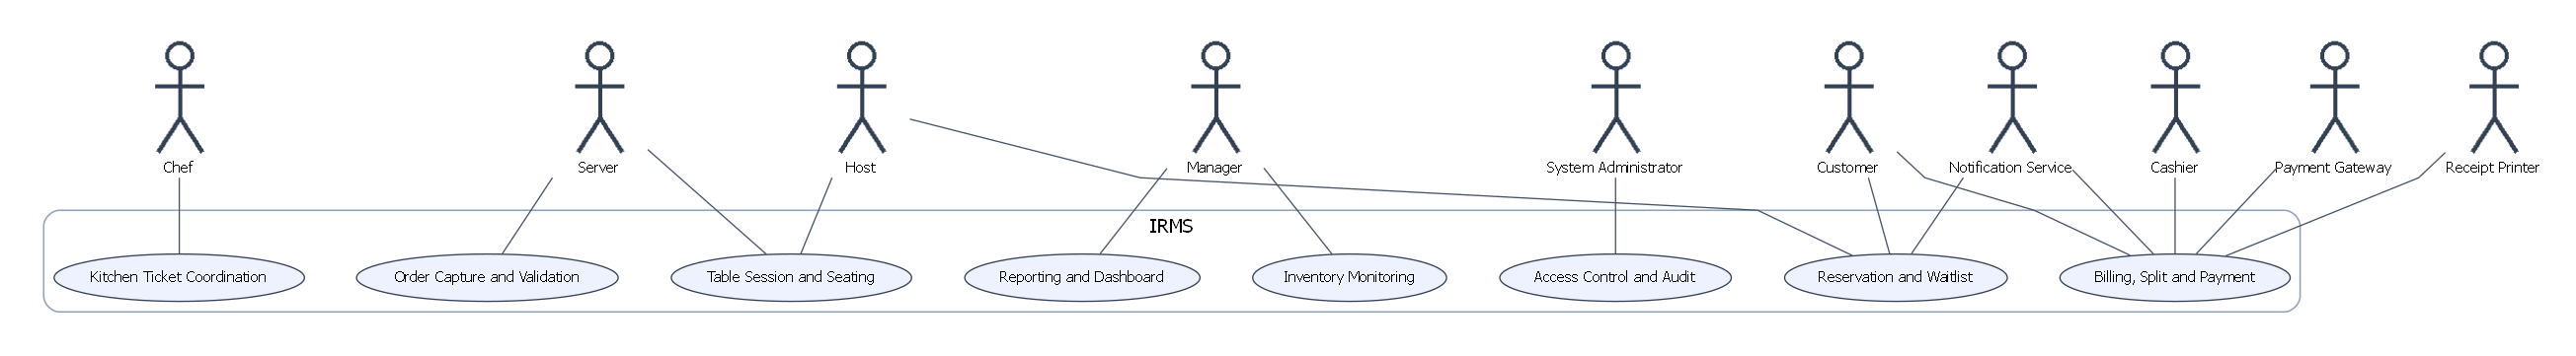
\includegraphics[width=\textwidth,height=0.84\textheight,keepaspectratio]{01_context_diagram_cua_irms.png}
\caption{Sơ đồ ngữ cảnh của IRMS}
\label{fig:irms-context-overview}
\end{figure}


Hình~\ref{fig:irms-context-overview} chốt rõ ranh giới hệ thống theo đúng kiểu \emph{context/process diagram}: IRMS được đặt ở trung tâm như một tiến trình điều phối duy nhất, còn xung quanh là các thực thể bên ngoài và hệ thống đối tác trao đổi dữ liệu với nó. Cách thể hiện này không chỉ trả lời câu hỏi \enquote{ai dùng IRMS}, mà còn làm rõ \enquote{dữ liệu gì đi vào, kết quả gì đi ra} ở từng điểm chạm như đặt bàn, xếp bàn, gọi món, điều phối bếp, quyết toán, kiểm soát truy cập và tích hợp dịch vụ ngoài.

\paragraph{Các điểm cần đọc từ sơ đồ ngữ cảnh.}
\begin{itemize}
  \item \textbf{Tuyến phục vụ phía trước}: \texttt{Customer}, \texttt{Host / Reception}, \texttt{Server / Floor Staff} và \texttt{Cashier} trao đổi trực tiếp các luồng dữ liệu thời gian thực như yêu cầu đặt bàn, trạng thái chờ, đơn gọi món, tách hóa đơn và nhập thông tin thanh toán.
  \item \textbf{Tuyến thực thi phía sau}: \texttt{Kitchen Operations} trả về trạng thái chế biến, tín hiệu món sẵn sàng hoặc hết nguyên liệu; \texttt{Manager} và \texttt{System Administrator} gửi thay đổi cấu hình, truy vấn báo cáo và yêu cầu kiểm toán ở lớp điều hành.
  \item \textbf{Các hợp đồng tích hợp ngoài}: \texttt{Payment Gateway}, \texttt{Notification Service} và \texttt{Receipt Printer} được đặt ngoài biên hệ thống để nhấn mạnh rằng thanh toán, gửi thông báo và in biên lai là các phụ thuộc cần được cách ly bằng giao tiếp có tên gọi rõ ràng.
  \item \textbf{Các luồng dữ liệu đều được đặt tên}: hình không dừng ở mức liệt kê vai trò, mà chỉ ra cụ thể các trao đổi như \enquote{reservation request}, \enquote{kitchen ticket}, \enquote{transaction result}, \enquote{audit trail} hoặc \enquote{print status}; nhờ đó ranh giới trách nhiệm của IRMS được khóa chặt hơn trước khi đi vào use case và kiến trúc.
\end{itemize}

Chính vì vậy, hình ngữ cảnh là cầu nối trực tiếp từ bối cảnh nghiệp vụ ở Chương 1 sang sơ đồ tổng quan kiến trúc ở Mục~\ref{sec:architecture-overview}: nó khóa ranh giới hệ thống trước khi tài liệu đi sâu vào cách phân rã các năng lực bên trong.

\begin{figure}[H]
\centering
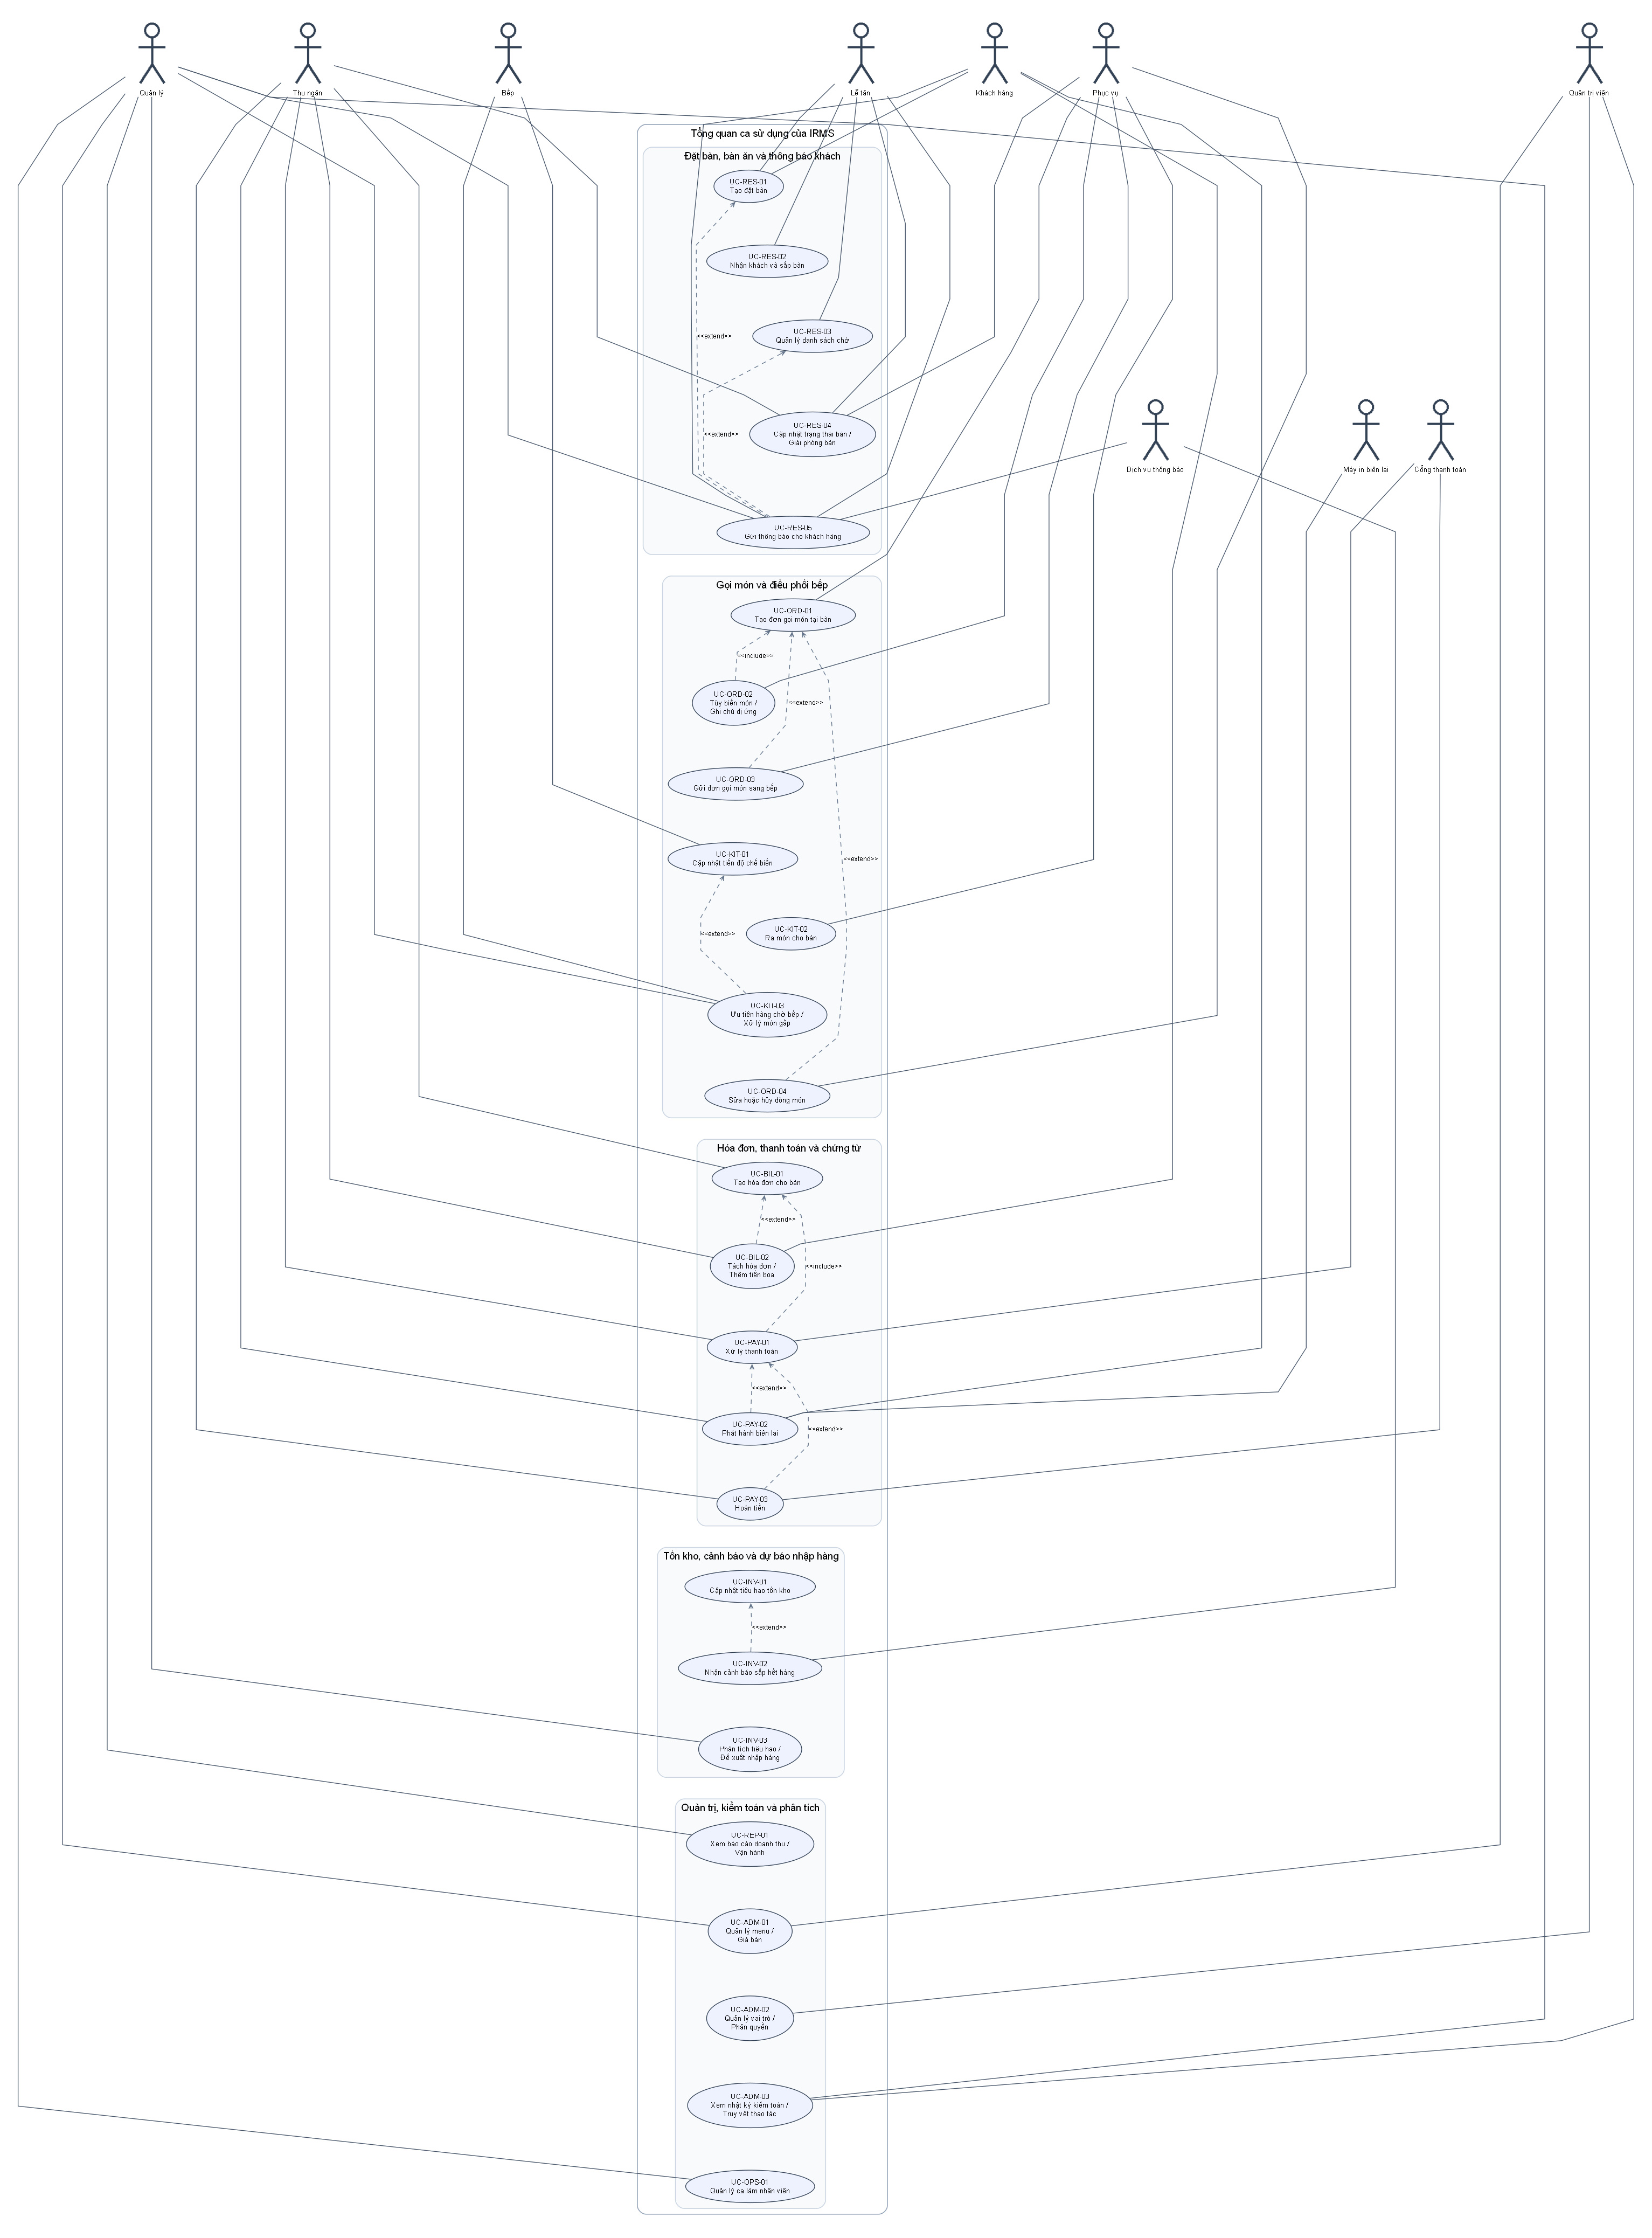
\includegraphics[width=\textwidth,height=0.84\textheight,keepaspectratio]{02_use_case_overview_cua_irms.png}
\caption{Sơ đồ tổng quan ca sử dụng của IRMS}
\label{fig:irms-usecase-overview}
\end{figure}


Hình~\ref{fig:irms-usecase-overview} trình bày tổng quan ca sử dụng theo đúng ký pháp UML: các actor đứng ngoài biên hệ thống, các ca sử dụng được biểu diễn bằng ellipse và được gom thành năm gói nghiệp vụ lớn gồm đặt bàn và vòng đời bàn, gọi món và điều phối bếp, hóa đơn và thanh toán, tồn kho và dự báo nhập hàng, cùng quản trị, kiểm toán và phân tích. Cách tổ chức này cho thấy phạm vi của IRMS không dừng ở các thao tác trực tiếp trước khách hàng, mà bao trùm cả phần kết thúc vòng đời bàn, giao tiếp chủ động với khách hàng, điều phối ưu tiên trong bếp, hỗ trợ quyết định nhập hàng từ dữ liệu tiêu hao lịch sử và truy vết thao tác nhạy cảm ở tầng quản trị.

Nhìn theo góc độ nghiệp vụ, năm cụm này cũng tương ứng với năm lớp trách nhiệm khác nhau trong hệ thống. Cụm đặt bàn và bàn ăn quản lý năng lực tiếp nhận khách theo thời gian thực; cụm gọi món và bếp điều khiển luồng thực thi nóng nhất của nhà hàng; cụm hóa đơn và thanh toán chốt quyết định tài chính; cụm tồn kho và dự báo hỗ trợ điều hành vật tư; còn cụm quản trị, kiểm toán và phân tích bảo đảm hệ thống có thể được kiểm soát, truy vết và cải tiến sau vận hành. Vì vậy, sơ đồ tổng quan ca sử dụng không chỉ là danh mục chức năng, mà còn là bản đồ chỉ ra nơi nào cần phản hồi tức thời, nơi nào cần độ đúng đắn cao, và nơi nào có thể chấp nhận xử lý sau trên tuyến nền.

\paragraph{Năm gói ca sử dụng chính thể hiện trong hình.}
\begin{itemize}
  \item \textbf{Reservation and Seating}: gom toàn bộ vòng đời đặt bàn, check-in, danh sách chờ, giải phóng bàn và thông báo cho khách.
  \item \textbf{Ordering and Kitchen}: gom tuyến gọi món, tùy biến món, điều phối bếp, cập nhật trạng thái chế biến và xử lý ưu tiên trong giờ cao điểm.
  \item \textbf{Billing and Payment}: gom các thao tác tạo hóa đơn, tách hóa đơn, thanh toán, phát hành biên lai và hoàn tiền.
  \item \textbf{Inventory and Reorder}: gom tiêu hao tồn kho, cảnh báo mức tồn thấp và hỗ trợ quyết định nhập hàng.
  \item \textbf{Governance and Analytics}: gom các ca sử dụng quản trị menu, phân quyền, nhật ký kiểm toán, báo cáo và lịch ca.
\end{itemize}

Việc gom theo gói ở mức tổng quan giúp hình giữ được khả năng đọc, còn phần chi tiết của từng mã ca sử dụng vẫn được triển khai ngay sau đó trong danh mục và các đặc tả cụ thể. Cách trình bày này cũng tạo nhịp chuyển hợp lý sang các góc nhìn logic và mô-đun ở chương kiến trúc, nơi năm gói nghiệp vụ này được ánh xạ thành các miền trách nhiệm ổn định hơn; phần định vị và giải thích mở rộng của sơ đồ tổng quan ca sử dụng được dẫn ngay tới Bảng~\ref{tab:appendix-traceability} và Bảng~\ref{tab:appendix-view-rationale}.

\begin{figure}[H]
\centering
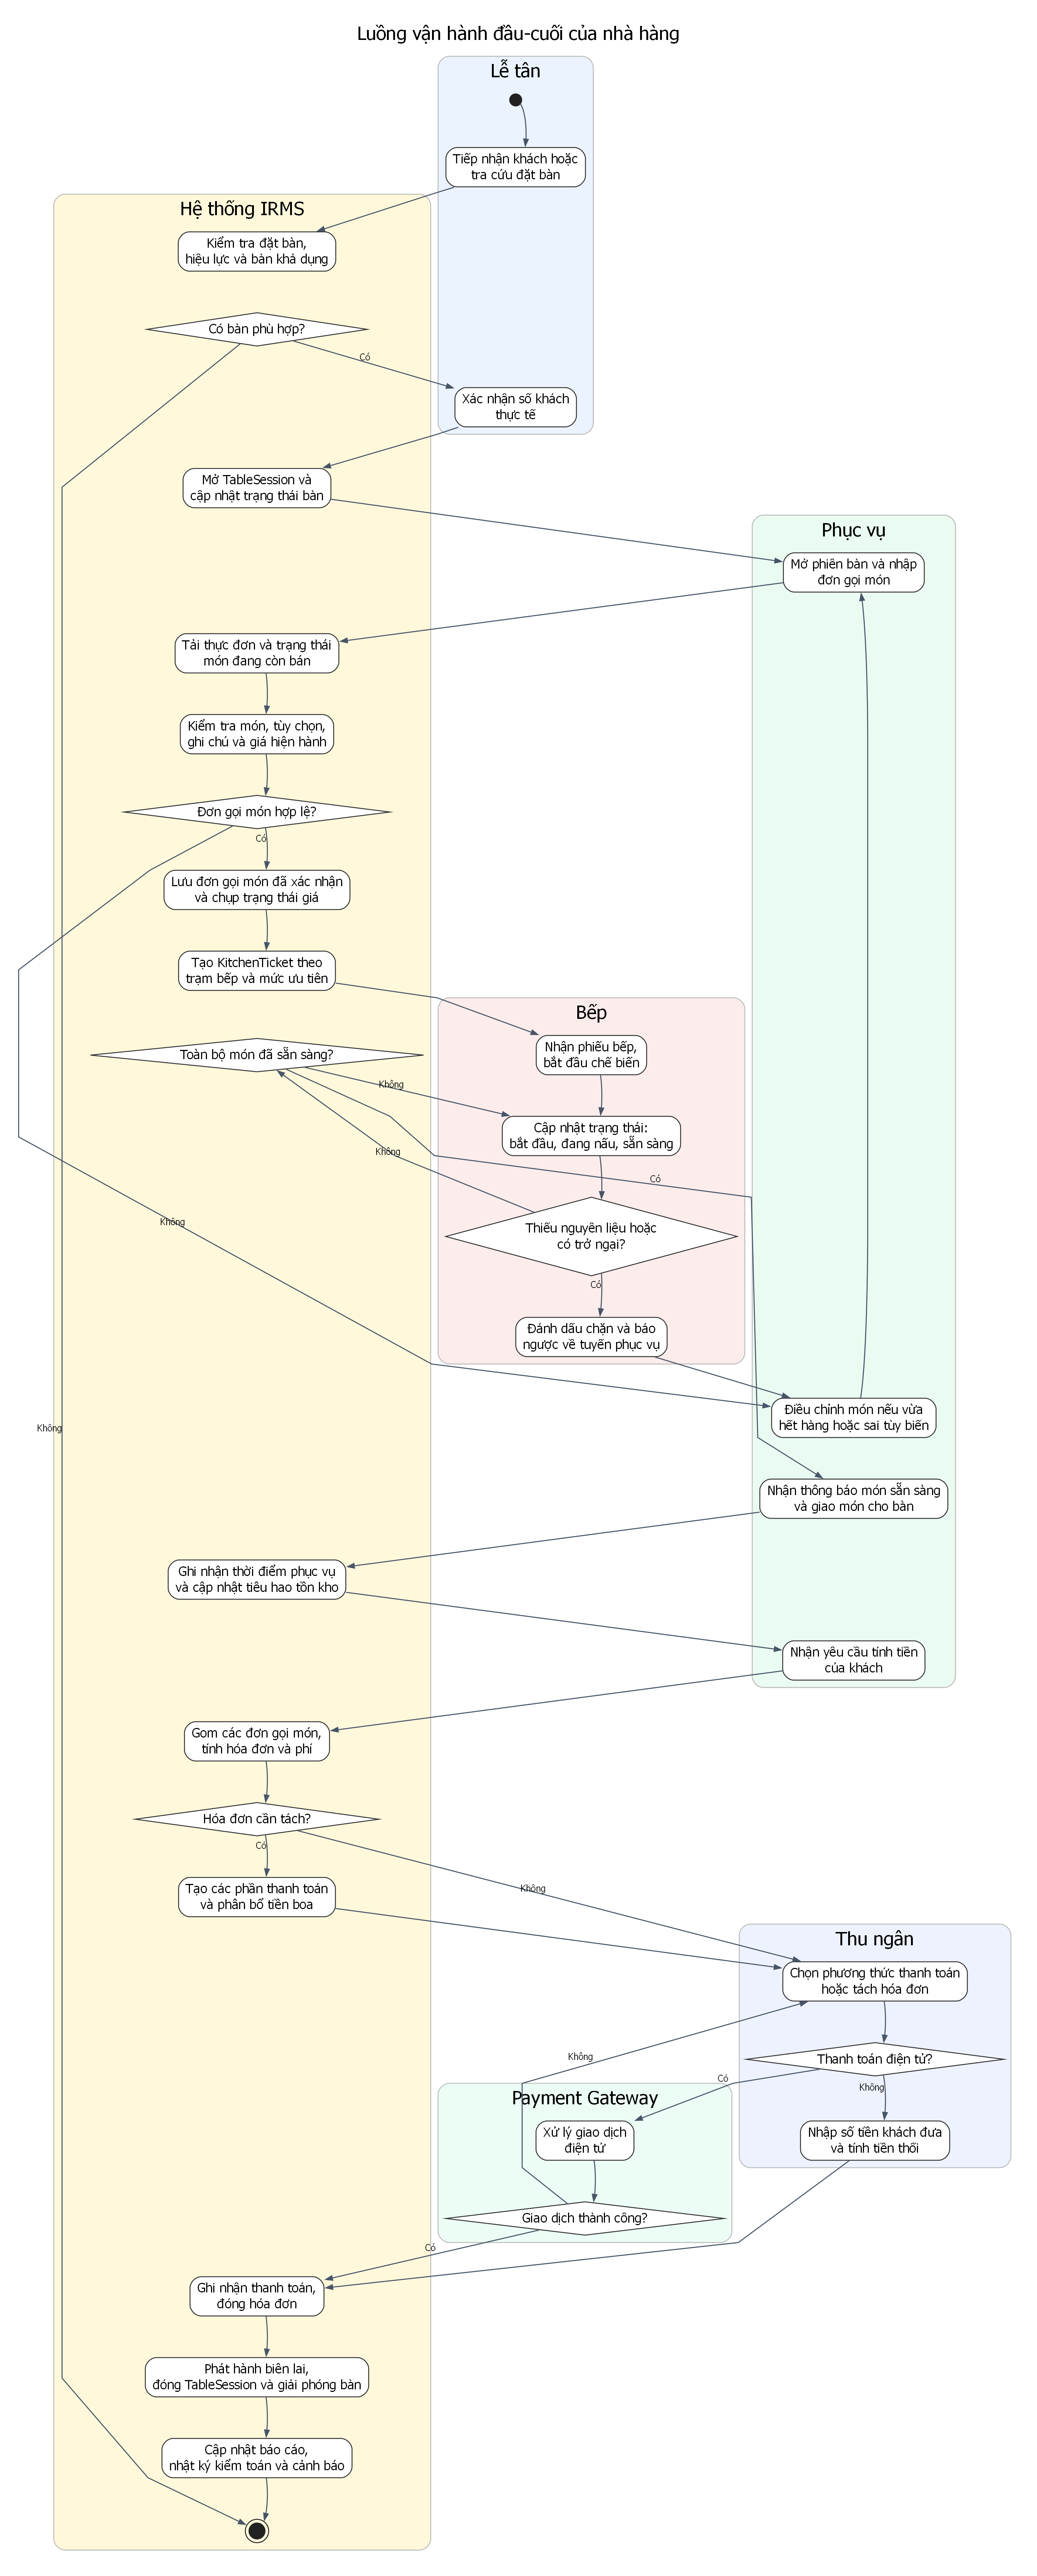
\includegraphics[width=\textwidth,height=0.84\textheight,keepaspectratio]{03_activity_diagram_end_to_end_restaurant_operation.png}
\caption{Sơ đồ hoạt động của luồng vận hành đầu-cuối nhà hàng}
\label{fig:irms-activity-end-to-end}
\end{figure}


Hình~\ref{fig:irms-activity-end-to-end} mô tả luồng vận hành đầu-cuối tiêu biểu của nhà hàng, bắt đầu từ khâu tiếp nhận khách hoặc kiểm tra đặt bàn, chuyển sang mở phiên bàn, tạo đơn gọi món, gửi phiếu xuống bếp, cập nhật tiến độ chế biến, giao món, lập hóa đơn, xử lý thanh toán và kết thúc bằng giải phóng bàn. Điểm quan trọng của sơ đồ hoạt động này là nó cho thấy những trạng thái nào phải được đồng bộ mạnh giữa các bộ phận: một bàn chỉ được mở một phiên phục vụ, một đơn đã xác nhận phải sinh phiếu bếp, và một hóa đơn chỉ được đóng khi thanh toán hoàn tất hoặc được ghi nhận là thất bại có kiểm soát.

Nhìn dưới góc độ kiến trúc, luồng đầu-cuối này cũng chỉ ra ranh giới giữa \textbf{đường giao dịch nóng} và \textbf{đường xử lý nền}. Các bước như xác nhận đơn gọi món, cập nhật trạng thái phiếu \texttt{Ready}, ghi nhận thanh toán thành công và đóng \texttt{TableSession} thuộc về tuyến đồng bộ bắt buộc vì chúng tác động trực tiếp đến trải nghiệm khách hàng. Ngược lại, các bước như cập nhật báo cáo, phát cảnh báo mức tồn thấp, gửi thông báo xác nhận hoặc đồng bộ số liệu quản trị có thể được đẩy sang luồng bất đồng bộ để giảm tải cho các điểm chạm thời gian thực.

\paragraph{Những mắt xích kiến trúc được khóa bởi sơ đồ đầu-cuối.}
\begin{itemize}
  \item \textbf{Điểm bàn giao giữa các khu vực}: lễ tân mở phiên bàn, phục vụ xác nhận đơn, bếp cập nhật trạng thái, thu ngân quyết toán; mỗi điểm bàn giao đều gắn với một thay đổi trạng thái có hậu quả nghiệp vụ.
  \item \textbf{Điểm đồng bộ bắt buộc}: mở \texttt{TableSession}, xác nhận đơn, đánh dấu món sẵn sàng, ghi nhận thanh toán và giải phóng bàn không được nhập nhằng về trạng thái.
  \item \textbf{Điểm bất đồng bộ chấp nhận được}: thông báo, báo cáo và một phần cảnh báo tồn kho được đẩy ra sau mà không làm sai tuyến phục vụ trước mặt khách hàng.
  \item \textbf{Điểm nối sang chương kiến trúc}: hình này là cơ sở để kiểm tra xem các sơ đồ logic, mô-đun, thành phần và triển khai ở chương sau có thật sự bảo vệ được luồng vận hành đầu-cuối hay không.
\end{itemize}

\begin{table}[H]
\centering
\caption{Danh mục 25 ca sử dụng chính được đặc tả chi tiết}
\begin{tabularx}{\textwidth}{>{\bfseries}p{4.0cm} X}
\toprule
Nhóm & Mã ca sử dụng \\
\midrule
Nhóm đặt bàn và bàn ăn & UC-RES-01, UC-RES-02, UC-RES-03, UC-RES-04, UC-RES-05 \\
Nhóm gọi món và điều phối bếp & UC-ORD-01, UC-ORD-02, UC-ORD-03, UC-KIT-01, UC-KIT-02, UC-KIT-03, UC-ORD-04 \\
Nhóm thanh toán & UC-BIL-01, UC-BIL-02, UC-PAY-01, UC-PAY-02, UC-PAY-03 \\
Nhóm tồn kho, cảnh báo và dự báo & UC-INV-01, UC-INV-02, UC-INV-03 \\
Nhóm quản trị, kiểm toán và phân tích & UC-REP-01, UC-ADM-01, UC-ADM-02, UC-ADM-03, UC-OPS-01 \\
\bottomrule
\end{tabularx}
\end{table}

Năm ca sử dụng giữ vai trò khóa kín phạm vi nghiệp vụ ở phần này là \texttt{UC-RES-04}, \texttt{UC-RES-05}, \texttt{UC-KIT-03}, \texttt{UC-INV-03} và \texttt{UC-ADM-03}. Chúng làm rõ các mắt xích dễ bị xem nhẹ khi mô tả hệ thống nhà hàng ở mức khái quát: kết thúc vòng đời bàn sau thanh toán, giao tiếp chủ động với khách hàng, điều phối ưu tiên trong bếp, hỗ trợ quyết định nhập hàng từ dữ liệu lịch sử và truy vết thao tác nhạy cảm ở tầng quản trị.

\subsection{Góc nhìn sử dụng}
Góc nhìn sử dụng cho thấy cách các tác nhân tương tác với các dịch vụ qua các kịch bản nghiệp vụ tiêu biểu.
Về mặt lý thuyết, góc nhìn sử dụng là công cụ rất tốt để \textbf{kiểm chứng kiến trúc bằng kịch bản}.
Một phương án phân rã đẹp trên góc nhìn mô-đun vẫn có thể thất bại khi đi qua tình huống thực,
nếu chuỗi tương tác quá dài, lỗi khó giải thích hoặc ranh giới giao dịch không rõ.
Do đó, bốn kịch bản dưới đây được chọn vì chúng chạm vào bốn luồng cốt lõi nhất của IRMS.

\subsubsection{Kịch bản 1: Từ đặt bàn đến tiếp nhận và xếp bàn}
\begin{enumerate}
  \item Khách hàng hoặc lễ tân tạo đặt bàn.
  \item \texttt{Reservation Service} kiểm tra khả dụng và gán bàn hoặc giữ chỗ.
  \item Khi khách đến, \texttt{Host UI} xác nhận tiếp nhận và mở \texttt{TableSession}.
  \item \texttt{TableSession} được chuyển tới \texttt{Server POS UI} để phục vụ gọi món.
\end{enumerate}

\subsubsection{Kịch bản 2: Từ gọi món đến điều phối bếp và phục vụ}
\begin{enumerate}
  \item Phục vụ tạo đơn gọi món và cấu hình tùy chọn món hoặc gợi ý dị ứng trên \texttt{Server POS UI}.
  \item \texttt{Ordering Service} xác nhận đơn gọi món và phát sự kiện tạo phiếu bếp.
  \item \texttt{Kitchen Coordination Service} tách phiếu theo trạm bếp và hiển thị lên \texttt{Kitchen Display UI}.
  \item Bếp cập nhật trạng thái từng dòng phiếu; màn hình gọi món nhận lại trạng thái sẵn sàng.
  \item Phục vụ giao món và đánh dấu đã phục vụ; \texttt{Inventory Service} nhận sự kiện để trừ tồn.
\end{enumerate}

\subsubsection{Kịch bản 3: Từ hóa đơn đến thanh toán và biên lai}
\begin{enumerate}
  \item Thu ngân hoặc phục vụ gom các đơn gọi món của bàn thành hóa đơn.
  \item \texttt{Billing Service} áp dụng khuyến mãi, tiền boa và tách hóa đơn nếu cần.
  \item Thanh toán được thực hiện qua tiền mặt hoặc cổng thanh toán điện tử.
  \item Khi thanh toán đủ, biên lai được phát hành và \texttt{TableSession} chuyển sang chuẩn bị đóng.
\end{enumerate}

\subsubsection{Kịch bản 4: Từ cảnh báo mức tồn thấp đến quyết định của quản lý}
\begin{enumerate}
  \item \texttt{Inventory Service} cập nhật lượng tồn thực tế sau mỗi món đã phục vụ hoặc sau mỗi lần điều chỉnh thủ công.
  \item Nếu xuống dưới ngưỡng, hệ thống tạo sự kiện cảnh báo mức tồn thấp.
  \item \texttt{Manager Portal} nhận cảnh báo, hiển thị nguyên liệu bị ảnh hưởng và món có nguy cơ hết hàng.
  \item Quản lý quyết định nhập thêm hàng hoặc tạm ẩn món trong menu.
\end{enumerate}

\begin{infobox}
\textbf{Giải thích chi tiết cho góc nhìn sử dụng.}
Góc nhìn sử dụng đặc biệt quan trọng với IRMS vì hệ thống không phải một khối xử lý tĩnh; nó là một chuỗi phối hợp giữa người và máy theo thời gian thực. Mỗi kịch bản ở trên đều cho thấy ranh giới nào cần đồng bộ mạnh, chẳng hạn như thanh toán, và ranh giới nào chấp nhận xử lý bất đồng bộ, chẳng hạn như báo cáo hoặc cảnh báo mức tồn thấp.
\end{infobox}

\begin{landscape}
\begin{figure}[H]
\centering
\IfFileExists{11_sequence_diagram_reservation_check_in_and_seating.pdf}{
  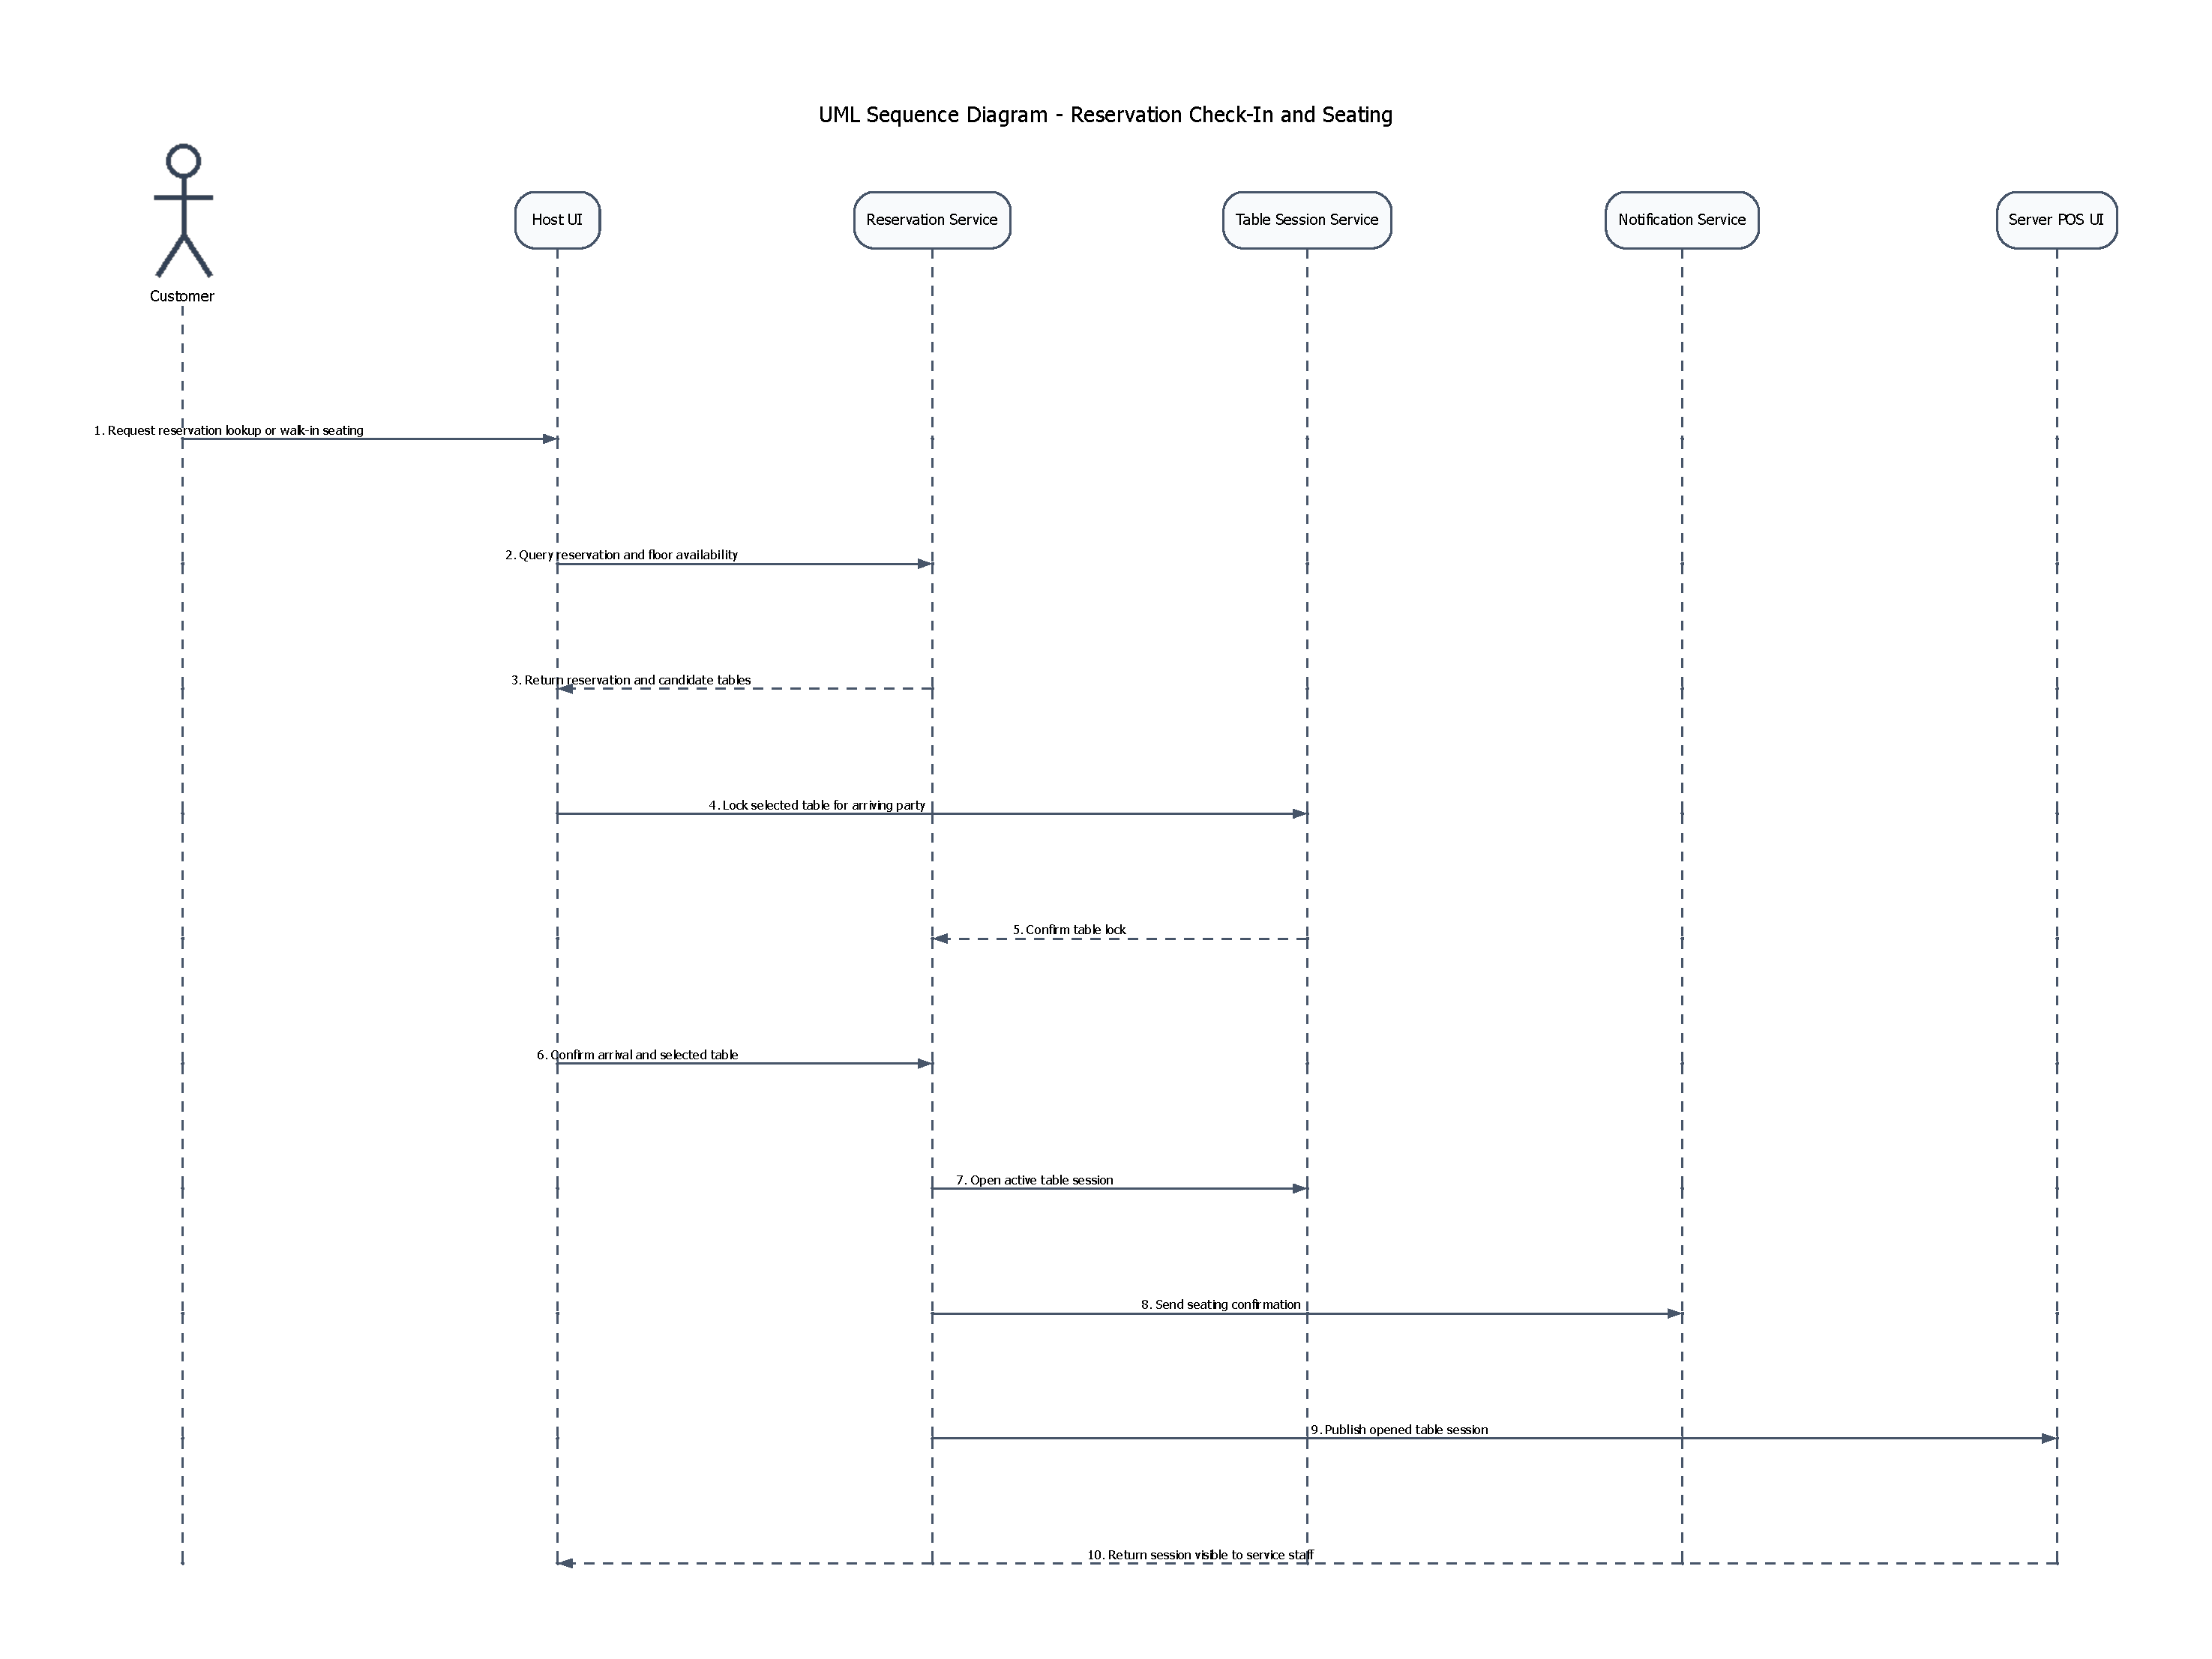
\includegraphics[width=0.97\linewidth,height=0.84\textheight,keepaspectratio]{11_sequence_diagram_reservation_check_in_and_seating.pdf}
}{
  \IfFileExists{11_sequence_diagram_reservation_check_in_and_seating.png}{
    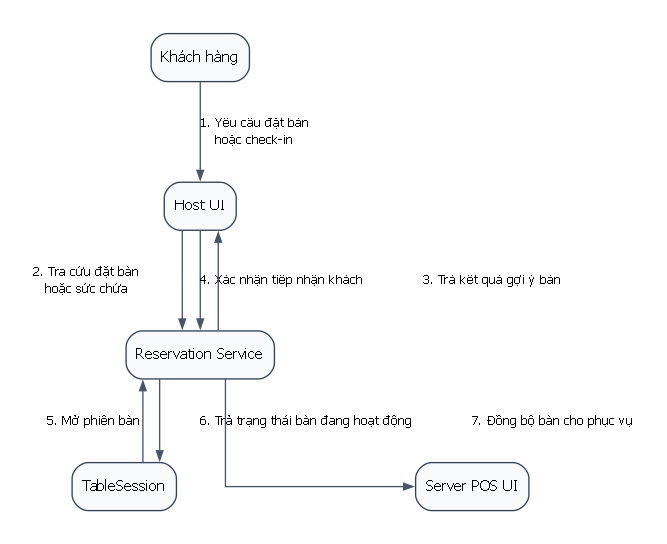
\includegraphics[width=0.97\linewidth,height=0.84\textheight,keepaspectratio]{11_sequence_diagram_reservation_check_in_and_seating.png}
  }{
    \fbox{\parbox{0.82\linewidth}{Thiếu file \texttt{11\_sequence\_diagram\_reservation\_check\_in\_and\_seating.(pdf/png)}.}}
  }
}
\caption{Sơ đồ trình tự cho kịch bản từ đặt bàn đến tiếp nhận và xếp bàn}
\label{fig:irms-usage-reservation}
\end{figure}
\end{landscape}


Hình~\ref{fig:irms-usage-reservation} cho thấy \texttt{Reservation} và \texttt{TableSession}
không phải là cùng một thực thể nghiệp vụ dù chúng liên quan trực tiếp.
Điểm mạnh của cách tách này là hệ thống xử lý được nhiều trường hợp thực tế:
khách có đặt bàn nhưng không đến,
khách vào trực tiếp không có đặt bàn nhưng vẫn mở phiên phục vụ,
hoặc lễ tân phải đổi bàn khi năng lực phục vụ thay đổi.
Nếu trộn hai khái niệm này thành một,
kiến trúc sẽ khó biểu diễn các trạng thái chuyển tiếp quan trọng của vận hành nhà hàng.

Đánh đổi là luồng xếp bàn phải cẩn thận hơn về đồng bộ trạng thái:
đặt bàn có thể còn hiệu lực nhưng bàn ăn chưa sẵn sàng;
bàn có thể vừa được giải phóng nhưng vẫn đang dọn dẹp;
thao tác tiếp nhận có thể đến muộn so với thời điểm giữ chỗ ban đầu.
Do đó, góc nhìn sử dụng này nhắc rằng đặt bàn và xếp bàn tuy nhìn đơn giản,
nhưng thực ra là nơi chứa nhiều quy tắc nghiệp vụ về thời gian và năng lực bàn.

\paragraph{Các thành phần chính thể hiện trong hình.}
\begin{itemize}
  \item \textbf{Khách hàng và Host UI}: khởi tạo yêu cầu đặt bàn hoặc check-in.
  \item \textbf{Reservation Service}: chịu trách nhiệm xác thực trạng thái đặt bàn và gợi ý bàn.
  \item \textbf{TableSession và Server POS UI}: nhận bàn đã mở để chuyển sang luồng phục vụ thực tế.
\end{itemize}

\paragraph{Lý do thiết kế của sơ đồ này.}
\begin{itemize}
  \item Sơ đồ làm rõ ranh giới giữa dữ liệu đặt bàn và phiên bàn thực tế.
  \item Đây là kịch bản giúp chứng minh tại sao bài toán xếp bàn cần được mô hình hóa riêng thay vì gộp vào một trạng thái bàn đơn giản.
\end{itemize}

\begin{landscape}
\begin{figure}[H]
\centering
\IfFileExists{12_sequence_diagram_place_order_to_kitchen.pdf}{
  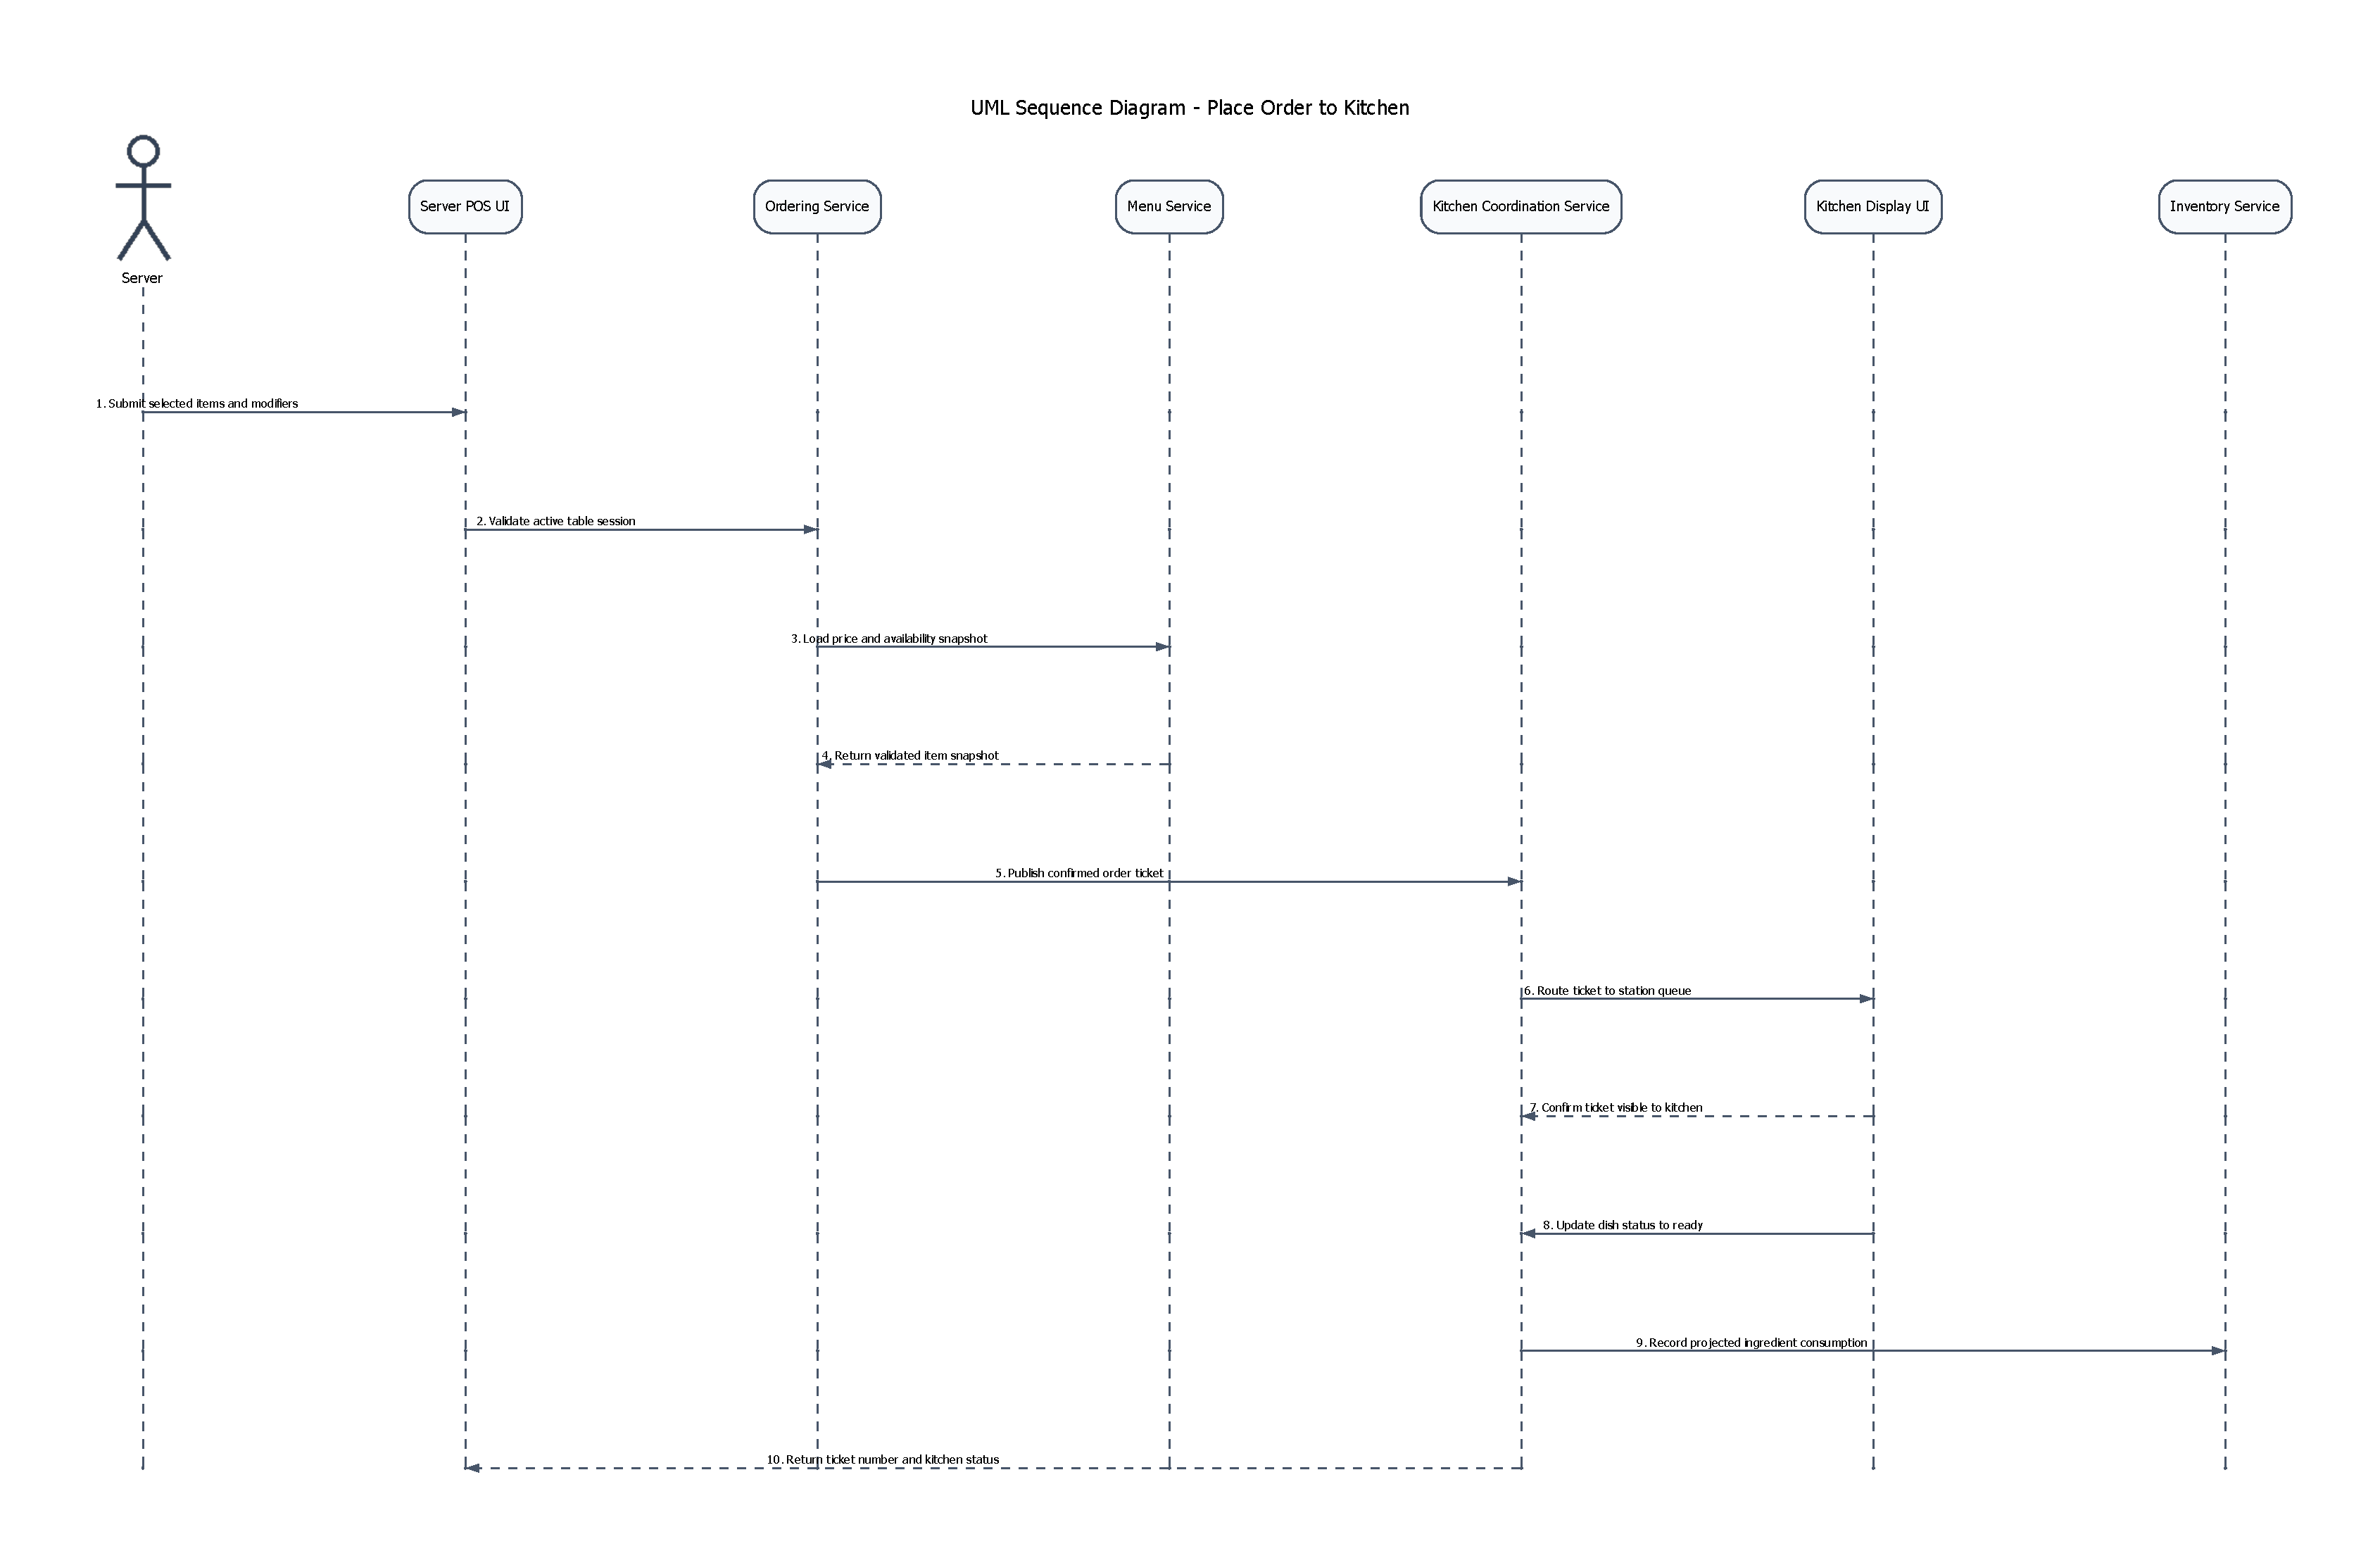
\includegraphics[width=0.97\linewidth,height=0.84\textheight,keepaspectratio]{12_sequence_diagram_place_order_to_kitchen.pdf}
}{
  \IfFileExists{12_sequence_diagram_place_order_to_kitchen.png}{
    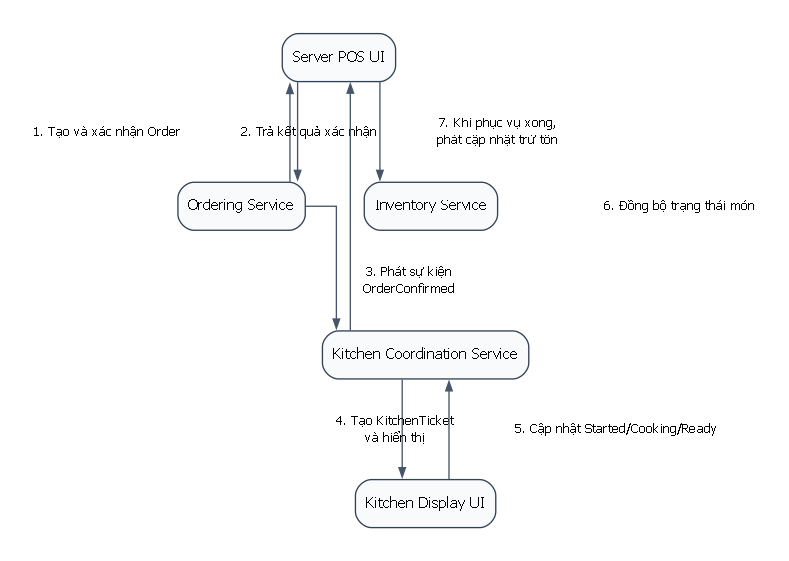
\includegraphics[width=0.97\linewidth,height=0.84\textheight,keepaspectratio]{12_sequence_diagram_place_order_to_kitchen.png}
  }{
    \fbox{\parbox{0.82\linewidth}{Thiếu file \texttt{12\_sequence\_diagram\_place\_order\_to\_kitchen.(pdf/png)}.}}
  }
}
\caption{Sơ đồ trình tự cho kịch bản từ gọi món đến điều phối bếp và phục vụ}
\label{fig:irms-usage-order-kitchen}
\end{figure}
\end{landscape}


Hình~\ref{fig:irms-usage-order-kitchen} là kịch bản quan trọng nhất để kiểm chứng \textbf{khả năng đáp ứng}.
Nguyên tắc thiết kế nên là:
\emph{lưu đơn gọi món thành công trước, rồi mới lan truyền sang bếp}.
Điều này bảo vệ tuyến đầu theo hai cách.
Thứ nhất, màn hình gọi món nhận phản hồi nhanh hơn vì không phải đợi toàn bộ chuỗi bếp, tồn kho và báo cáo.
Thứ hai, khi việc chuyển sang bếp gặp trục trặc,
hệ thống vẫn có thể thử lại từ trạng thái đơn đã xác nhận thay vì mất dữ liệu đơn gọi món.

Ưu điểm của mô hình này là tách được
\textbf{bước chốt giao dịch} khỏi \textbf{bước lan truyền vận hành}.
Tuy nhiên, đánh đổi là màn hình bếp và màn hình gọi món phải xử lý được trạng thái trung gian:
đơn đã xác nhận nhưng phiếu chưa hiện lên màn hình bếp ngay lập tức;
một dòng món có thể đã sẵn sàng ở bếp nhưng màn hình gọi món chưa nhận được cập nhật cuối cùng;
việc trừ tồn cũng có thể đi sau sự kiện phục vụ xong.
Vì thế, góc nhìn sử dụng này là bằng chứng rằng cơ chế nhất quán trễ ở IRMS phải được dùng có kiểm soát, không dùng tùy tiện.

\paragraph{Các thành phần chính thể hiện trong hình.}
\begin{itemize}
  \item \textbf{Server POS UI}: là điểm bắt đầu của thao tác gọi món.
  \item \textbf{Ordering Service}: là nơi chốt giao dịch gọi món.
  \item \textbf{Kitchen Coordination Service và Kitchen Display UI}: nhận luồng lan truyền sang bếp sau khi đơn đã được xác nhận.
  \item \textbf{Inventory Service}: chỉ nhận cập nhật sau khi món đã đi qua luồng phục vụ phù hợp.
\end{itemize}

\paragraph{Lý do thiết kế của sơ đồ này.}
\begin{itemize}
  \item Sơ đồ này nhấn mạnh thứ tự \enquote{xác nhận trước, lan truyền sau} của tuyến gọi món.
  \item Đây là kịch bản quan trọng nhất để giải thích vì sao kiến trúc phải cân bằng giữa phản hồi nhanh và nhất quán có kiểm soát.
\end{itemize}

\begin{landscape}
\begin{figure}[H]
\centering
\IfFileExists{13_sequence_diagram_checkout_and_payment.pdf}{
  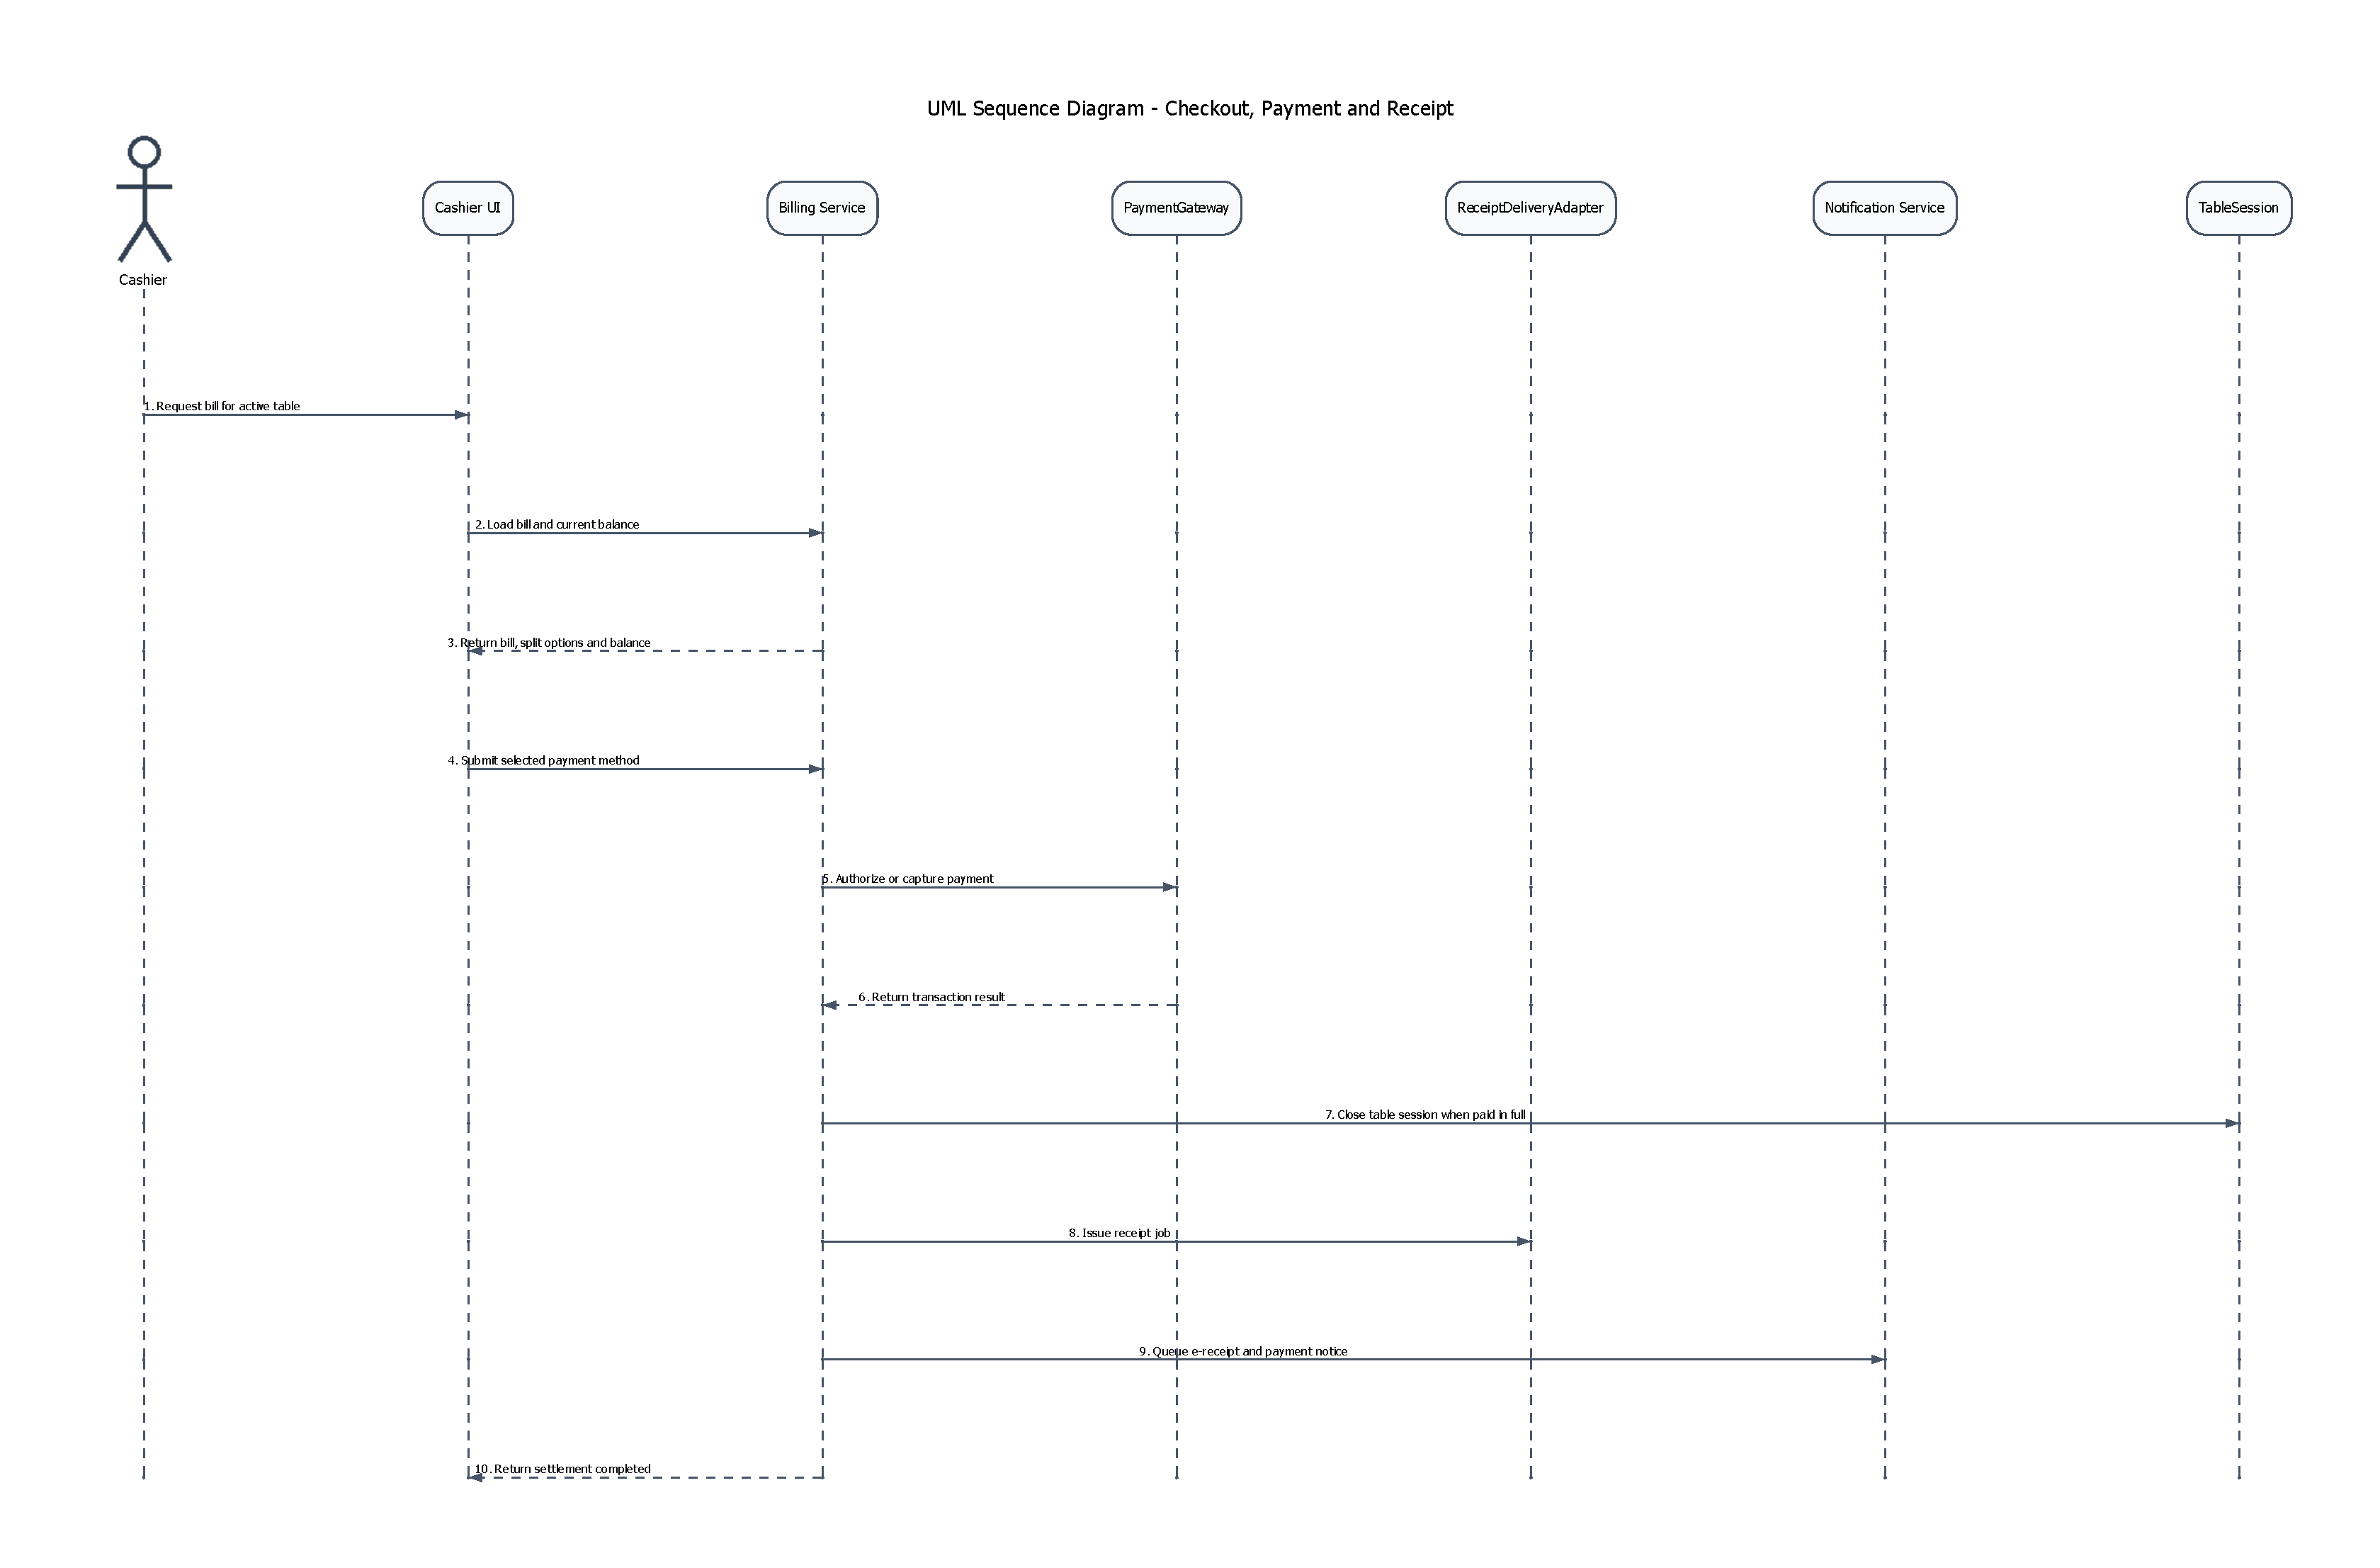
\includegraphics[width=0.97\linewidth,height=0.84\textheight,keepaspectratio]{13_sequence_diagram_checkout_and_payment.pdf}
}{
  \IfFileExists{13_sequence_diagram_checkout_and_payment.png}{
    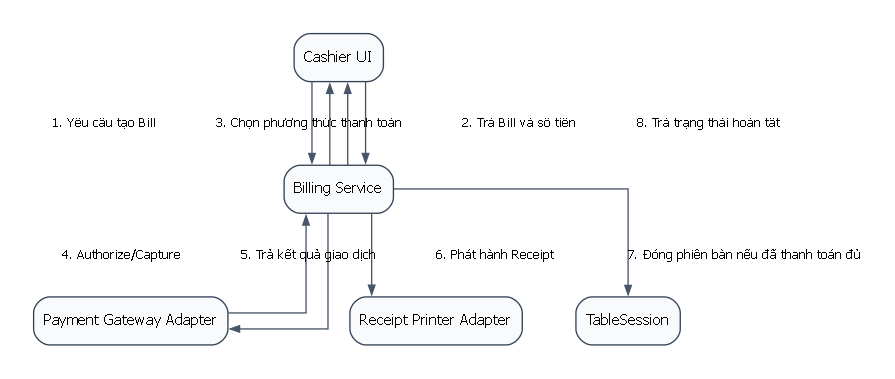
\includegraphics[width=0.97\linewidth,height=0.84\textheight,keepaspectratio]{13_sequence_diagram_checkout_and_payment.png}
  }{
    \fbox{\parbox{0.82\linewidth}{Thiếu file \texttt{13\_sequence\_diagram\_checkout\_and\_payment.(pdf/png)}.}}
  }
}
\caption{Sơ đồ trình tự cho kịch bản từ hóa đơn đến thanh toán và biên lai}
\label{fig:irms-usage-payment}
\end{figure}
\end{landscape}


Hình~\ref{fig:irms-usage-payment} là nơi kiến trúc phải nghiêng mạnh về \textbf{độ tin cậy}.
Ở kịch bản này, khối lập hóa đơn không chỉ làm phép cộng cuối cùng,
mà còn là nơi áp dụng khuyến mãi, tiền boa, tách hóa đơn, chọn phương thức thanh toán,
giao tiếp với cổng thanh toán, phát hành biên lai và đổi trạng thái phiên phục vụ.
Đây là luồng có mật độ chuyển trạng thái cao nhất và hệ quả nghiệp vụ lớn nhất nếu xử lý sai.

Ưu điểm của việc giữ thanh toán trong luồng đồng bộ là hệ thống có thể trả lời rất rõ:
giao dịch thành công hay thất bại, hóa đơn còn mở hay đã đóng, phiên phục vụ còn tiếp diễn hay đã kết thúc.
Ngược lại, nếu thanh toán bị đẩy sang bất đồng bộ quá mức,
thu ngân và khách hàng sẽ rất khó hiểu trạng thái thật sự của giao dịch.
Nhược điểm của cách làm đồng bộ là đường xử lý thanh toán trở thành điểm nhạy cảm với hệ ngoài,
đặc biệt khi cổng thanh toán chậm hoặc lỗi.
Vì thế, đây là nơi cần thời gian chờ rõ ràng, khóa chống xử lý lặp, nhật ký kiểm toán và cơ chế xử lý lỗi minh bạch nhất.

\paragraph{Các thành phần chính thể hiện trong hình.}
\begin{itemize}
  \item \textbf{Cashier UI}: là điểm điều khiển nghiệp vụ của thu ngân.
  \item \textbf{Billing Service}: giữ trung tâm của tuyến quyết toán.
  \item \textbf{Payment Gateway Adapter}: đại diện cho tích hợp thanh toán ngoài hệ thống.
  \item \textbf{Receipt Printer Adapter và TableSession}: kết thúc luồng bằng phát hành biên lai và đóng phiên bàn.
\end{itemize}

\paragraph{Lý do thiết kế của sơ đồ này.}
\begin{itemize}
  \item Đây là luồng nhạy cảm nhất về độ đúng đắn nghiệp vụ, nên cần được tách riêng để làm rõ ranh giới trách nhiệm và ranh giới giao dịch.
  \item Việc tách rõ cổng thanh toán, phát hành biên lai và đóng phiên bàn giúp người đọc thấy ranh giới trách nhiệm của từng bước sau khi thanh toán hoàn tất.
\end{itemize}

\begin{landscape}
\begin{figure}[H]
\centering
\IfFileExists{14_sequence_diagram_stock_update_and_low_stock_alert.pdf}{
  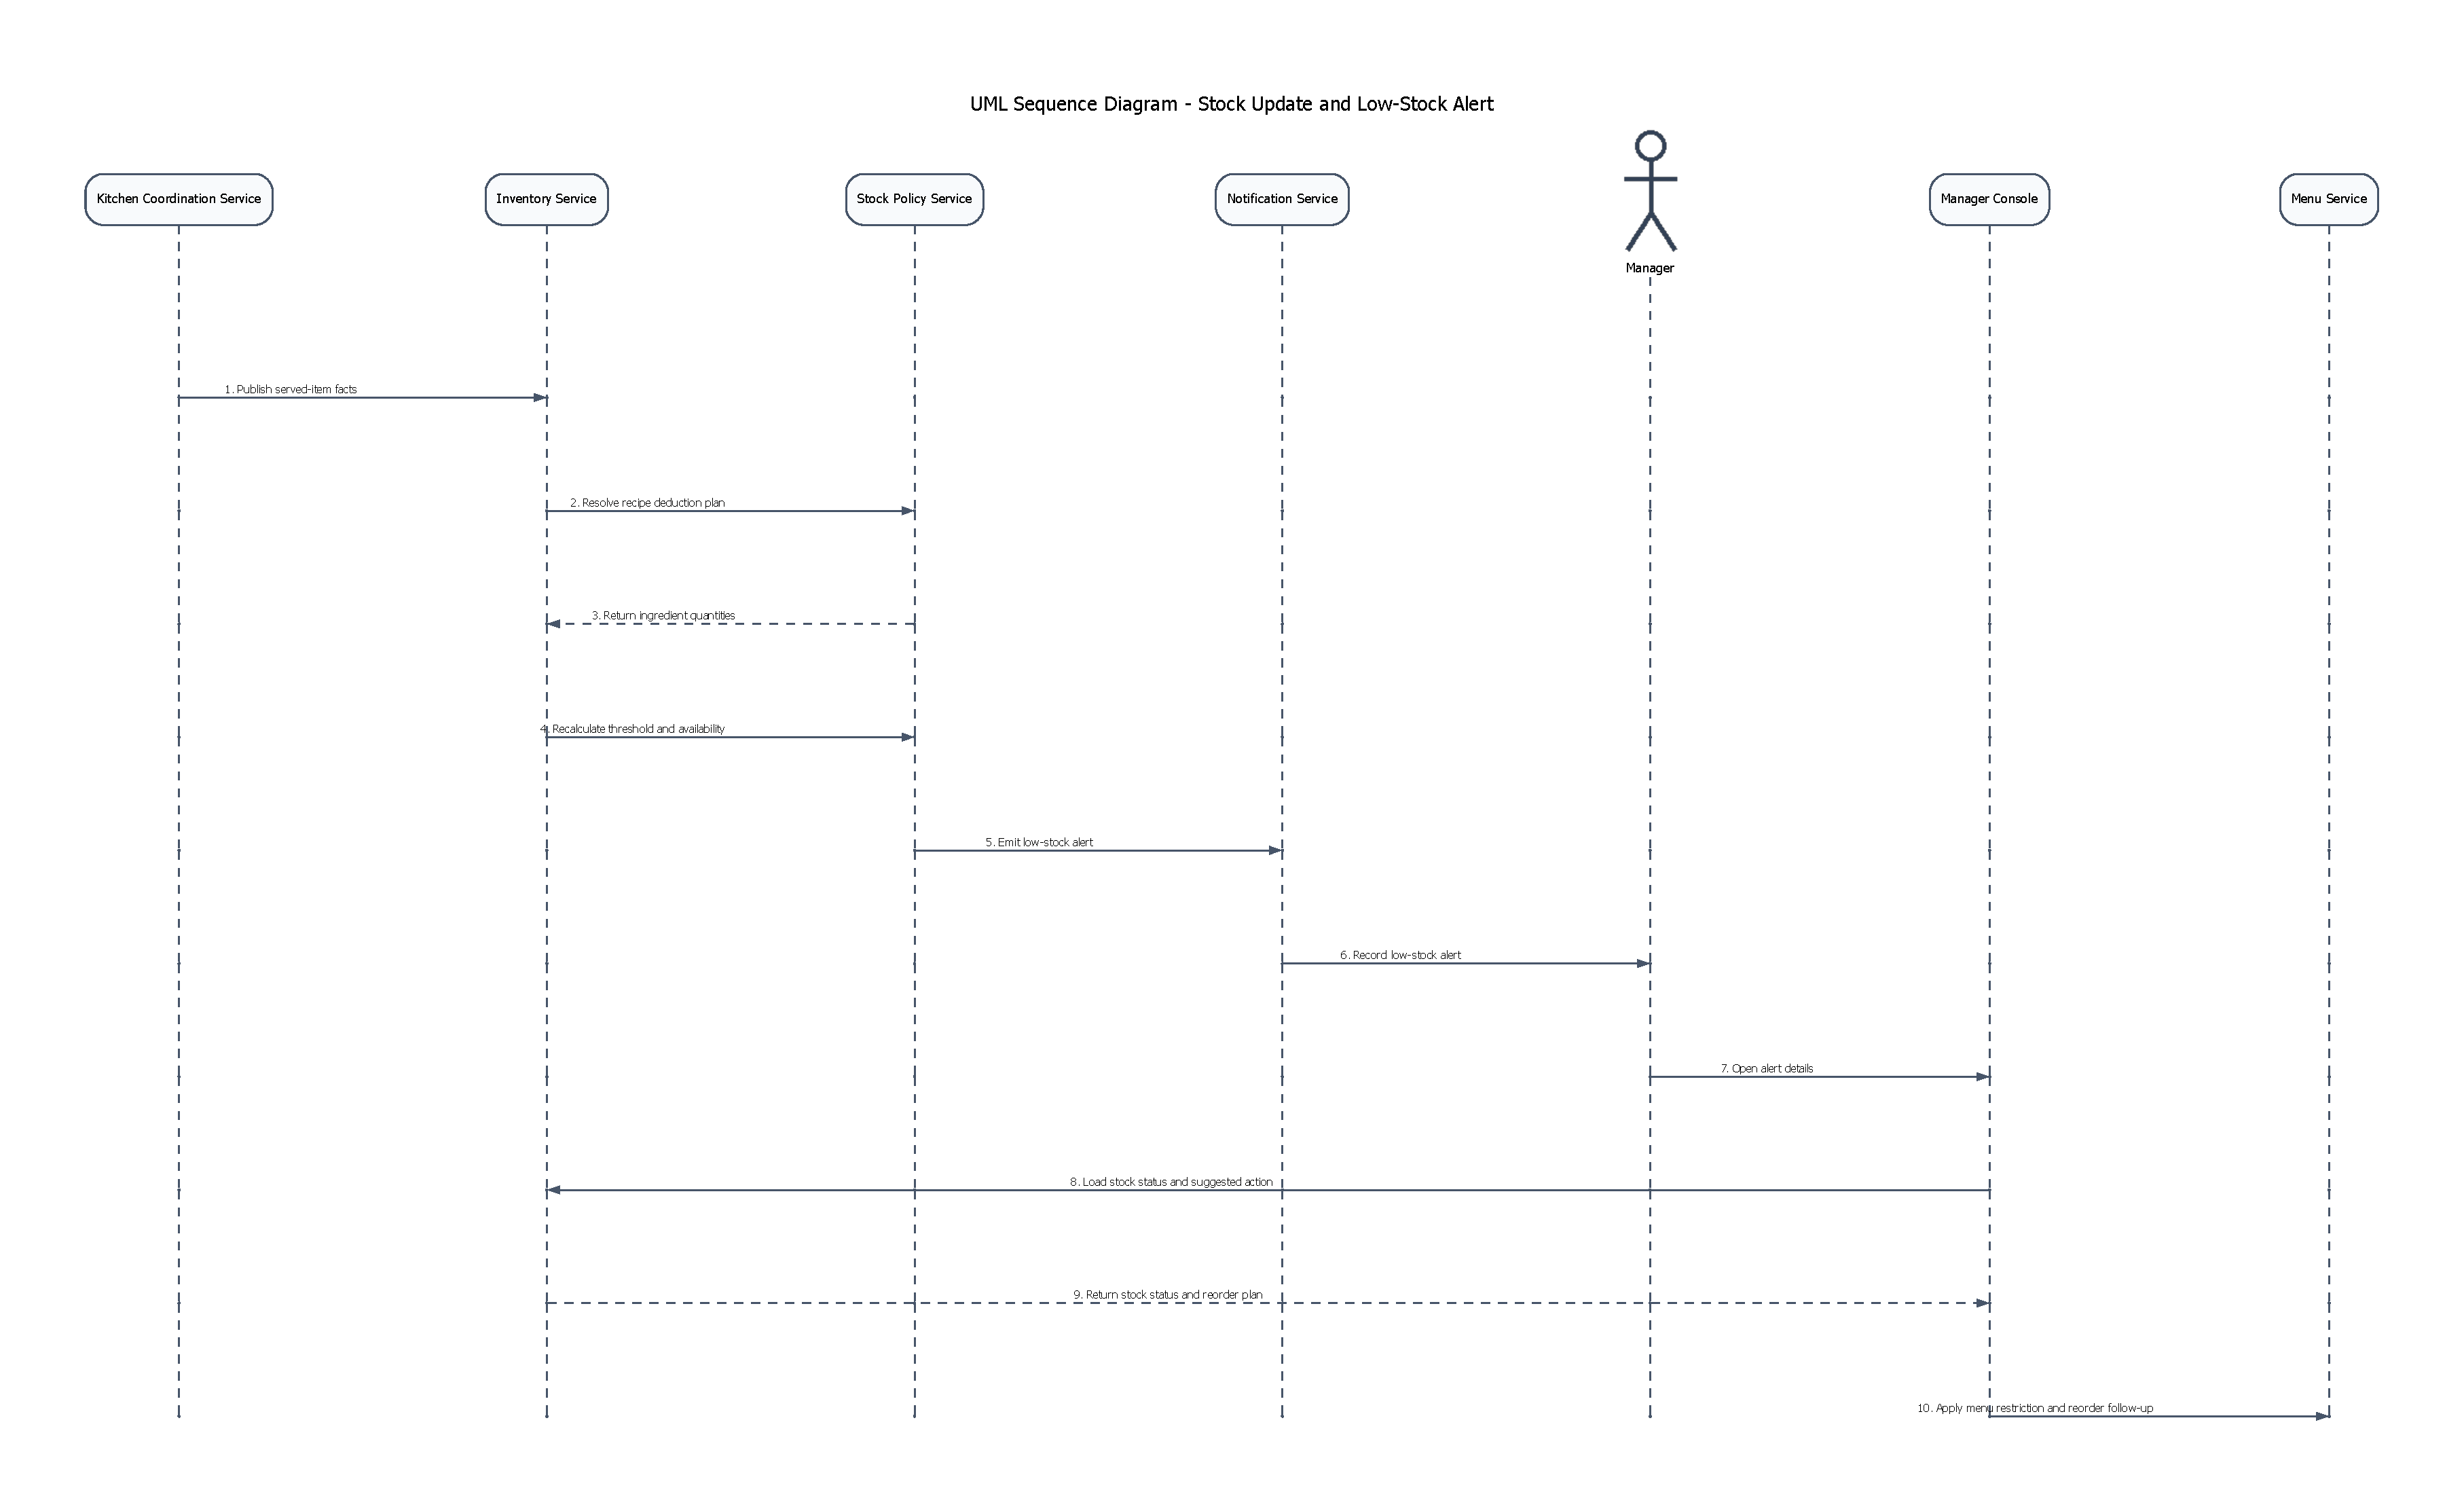
\includegraphics[width=0.97\linewidth,height=0.84\textheight,keepaspectratio]{14_sequence_diagram_stock_update_and_low_stock_alert.pdf}
}{
  \IfFileExists{14_sequence_diagram_stock_update_and_low_stock_alert.png}{
    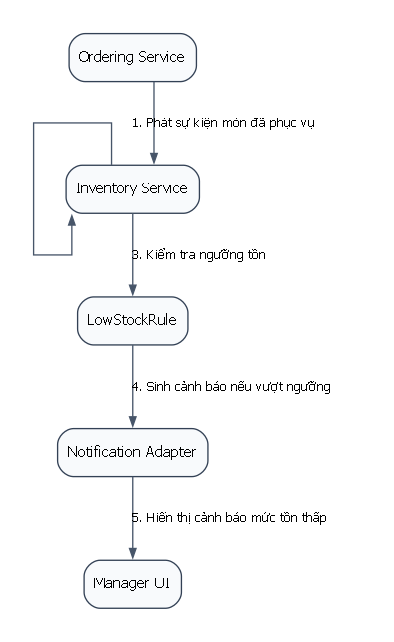
\includegraphics[width=0.97\linewidth,height=0.84\textheight,keepaspectratio]{14_sequence_diagram_stock_update_and_low_stock_alert.png}
  }{
    \fbox{\parbox{0.82\linewidth}{Thiếu file \texttt{14\_sequence\_diagram\_stock\_update\_and\_low\_stock\_alert.(pdf/png)}.}}
  }
}
\caption{Sơ đồ trình tự cho kịch bản từ cảnh báo mức tồn thấp đến quyết định của quản lý}
\label{fig:irms-usage-stock}
\end{figure}
\end{landscape}


Hình~\ref{fig:irms-usage-stock} cho thấy rõ vì sao quản lý tồn kho và gửi thông báo không nên chen trực tiếp vào tuyến giao dịch nóng.
Việc theo dõi tồn kho cần chính xác ở mức vận hành,
nhưng không nhất thiết phải khóa trải nghiệm gọi món của phục vụ
chỉ vì một cảnh báo quản lý chưa được gửi xong.
Cách đặt việc trừ tồn và cảnh báo mức tồn thấp trên luồng sự kiện
giúp hệ thống giữ được \textbf{khả năng sửa đổi}:
khi chính sách trừ kho, ánh xạ công thức hay ngưỡng cảnh báo thay đổi,
phần ảnh hưởng chủ yếu nằm trong khối tồn kho và khối gửi thông báo.

Nhược điểm là lượng tồn hiển thị cho quản lý có thể hơi chậm so với giao dịch mới nhất
nếu bộ xử lý nền bị trễ hoặc sự kiện đang được thử lại.
Điều này chấp nhận được trong phạm vi IRMS,
miễn là không nhầm lẫn cảnh báo tồn kho với xác nhận thanh toán.
Nói cách khác, góc nhìn sử dụng này giúp chứng minh nơi nào được phép chấp nhận độ trễ đồng bộ,
và nơi nào thì tuyệt đối không nên chấp nhận điều đó.

\paragraph{Các thành phần chính thể hiện trong hình.}
\begin{itemize}
  \item \textbf{Ordering Service}: là nguồn phát sinh biến động vận hành cần suy diễn sang kho.
  \item \textbf{Inventory Service và LowStockRule}: chịu trách nhiệm cập nhật tồn và đánh giá ngưỡng cảnh báo.
  \item \textbf{Notification Adapter và Manager UI}: là đầu ra quản trị của luồng cảnh báo.
\end{itemize}

\paragraph{Lý do thiết kế của sơ đồ này.}
\begin{itemize}
  \item Sơ đồ cho thấy rõ tồn kho và cảnh báo nên đi trên một tuyến hỗ trợ thay vì chen vào đường giao dịch nóng.
  \item Đây là ví dụ rõ nhất để giải thích sự khác nhau giữa \textbf{đúng về vận hành} và \textbf{phải phản hồi tức thời} trong kiến trúc.
\end{itemize}

\subsection{Đặc tả ca sử dụng}


\usepackage{longtable}
\usepackage{enumitem}

\renewcommand{\arraystretch}{1.3}

\begin{longtable}{|p{4cm}|p{10cm}|}
\hline
\textbf{Use Case ID} & UC-RES-01 \\ \hline
\textbf{Use Case Name} & Tạo đặt bàn \\ \hline
\textbf{Primary Actors} & Khách hàng, Lễ tân \\ \hline

\textbf{Description} & Tạo một đặt bàn hợp lệ cho ngày, giờ và số lượng khách cụ thể. \\ \hline

\textbf{Trigger} & Khách hàng gửi yêu cầu đặt bàn qua quầy lễ tân, điện thoại hoặc web/app. \\ \hline

\textbf{Preconditions} &
\begin{itemize}[leftmargin=*, noitemsep]
  \item Nhà hàng có mở nhận đặt bàn trong khung giờ yêu cầu.
  \item Có tối thiểu tên và số điện thoại khách hàng.
  \item Sơ đồ bàn và năng lực phục vụ đã được cấu hình.
\end{itemize} \\ \hline

\textbf{Postconditions} &
\begin{itemize}[leftmargin=*, noitemsep]
  \item Tạo đặt bàn với trạng thái \texttt{Pending} hoặc \texttt{Confirmed}.
  \item Hệ thống giữ chỗ hoặc gợi ý bàn phù hợp.
  \item Khách nhận mã đặt bàn và thông báo xác nhận.
\end{itemize} \\ \hline

\textbf{Normal Flow} &
\begin{enumerate}[leftmargin=*, noitemsep]
  \item Lễ tân nhập thời gian, số khách, tên và số điện thoại.
  \item Hệ thống kiểm tra và validate dữ liệu đầu vào.
  \item Hệ thống kiểm tra sức chứa, bàn trống và xung đột đặt bàn.
  \item Hệ thống gợi ý bàn hoặc nhóm bàn phù hợp.
  \item Lễ tân chọn bàn và nhập ghi chú nếu có.
  \item Hệ thống tạo đặt bàn và sinh mã đặt bàn.
  \item Hệ thống gửi thông báo xác nhận cho khách.
\end{enumerate} \\ \hline

\textbf{Alternative Flows} &
\begin{minipage}[t]{\linewidth}
\textbf{A1. Không đủ sức chứa (từ bước 3)} \\
3.1 Hệ thống đề xuất khung giờ khác hoặc đưa khách vào danh sách chờ.

\vspace{0.5em}
\textbf{A2. Yêu cầu đặc biệt (từ bước 4)} \\
4.1 Lễ tân lọc danh sách bàn theo khu vực hoặc thuộc tính yêu cầu.

\vspace{0.5em}
\textbf{A3. Không gán được bàn (từ bước 5)} \\
5.1 Hệ thống tạo đặt bàn trạng thái \texttt{Pending} và giữ chỗ theo số lượng khách.
\end{minipage} \\ \hline

\textbf{Exception Flows} &
\begin{minipage}[t]{\linewidth}
\textbf{E1. Dữ liệu không hợp lệ (từ bước 2)} \\
2.1 Hệ thống yêu cầu nhập lại thông tin khách.

\vspace{0.5em}
\textbf{E2. Lỗi đồng bộ sơ đồ bàn (từ bước 3)} \\
3.2 Hệ thống khóa thao tác và yêu cầu tải lại dữ liệu.
\end{minipage} \\ \hline

\textbf{Business Rules} &
\begin{itemize}[leftmargin=*, noitemsep]
  \item Không vượt quá sức chứa tối đa của bàn hoặc nhóm bàn.
  \item Nhóm khách lớn phải được xác nhận bởi lễ tân hoặc quản lý.
\end{itemize} \\ \hline

\end{longtable}



   \renewcommand{\arraystretch}{1.3}

\begin{longtable}{|p{4cm}|p{10cm}|}
\hline
\textbf{Use Case ID} & UC-RES-02 \\ \hline
\textbf{Use Case Name} & Nhận khách và sắp bàn \\ \hline
\textbf{Primary Actors} & Lễ tân, Phục vụ \\ \hline

\textbf{Description} & Tiếp nhận khách đến nhà hàng và gán khách vào bàn hoặc nhóm bàn phù hợp. \\ \hline

\textbf{Trigger} & Khách đến quầy lễ tân hoặc được gọi từ danh sách chờ. \\ \hline

\textbf{Preconditions} &
\begin{itemize}[leftmargin=*, noitemsep]
  \item Khách có đặt bàn hoặc có thể được xếp chỗ tại chỗ.
  \item Sơ đồ bàn và trạng thái bàn được đồng bộ theo thời gian thực.
\end{itemize} \\ \hline

\textbf{Postconditions} &
\begin{itemize}[leftmargin=*, noitemsep]
  \item Một phiên phục vụ bàn (\texttt{TableSession}) được mở.
  \item Bàn được chuyển sang trạng thái \texttt{Occupied} hoặc \texttt{Reserved-Arrived}.
  \item Phục vụ nhận được thông báo tiếp nhận bàn mới.
\end{itemize} \\ \hline

\textbf{Normal Flow} &
\begin{enumerate}[leftmargin=*, noitemsep]
  \item Lễ tân tìm đặt bàn theo mã, số điện thoại hoặc tên khách.
  \item Hệ thống hiển thị thông tin đặt bàn, trạng thái, thời điểm đến và bàn gợi ý.
  \item Lễ tân xác nhận khách đến, số khách thực tế và thời gian check-in.
  \item Hệ thống kiểm tra hiệu lực đặt bàn và trạng thái bàn.
  \item Lễ tân điều chỉnh hoặc ghép bàn nếu số lượng khách thay đổi.
  \item Hệ thống mở phiên phục vụ (\texttt{TableSession}).
  \item Hệ thống cập nhật trạng thái bàn thành \texttt{Occupied} hoặc \texttt{Reserved-Arrived}.
  \item Hệ thống phân công bàn cho phục vụ theo khu vực.
  \item Phục vụ nhận thông báo và chuẩn bị phục vụ.
\end{enumerate} \\ \hline

\textbf{Alternative Flows} &
\begin{minipage}[t]{\linewidth}

\textbf{A1. Khách vãng lai (từ bước 1)} \\
1.1 Lễ tân chọn chức năng xếp bàn trực tiếp. \\
1.2 Hệ thống gợi ý bàn trống phù hợp. \\
1.3 Lễ tân chọn bàn và tiếp tục từ bước 5.

\vspace{0.5em}
\textbf{A2. Thay đổi số lượng khách (từ bước 3)} \\
3.1 Lễ tân cập nhật số khách thực tế. \\
3.2 Hệ thống gợi ý lại bàn phù hợp hoặc yêu cầu ghép bàn.

\end{minipage} \\ \hline

\textbf{Exception Flows} &
\begin{minipage}[t]{\linewidth}

\textbf{E1. Bàn chưa sẵn sàng (từ bước 4)} \\
4.1 Hệ thống đề xuất bàn thay thế hoặc đưa khách vào danh sách chờ.

\vspace{0.5em}
\textbf{E2. Đặt bàn hết hiệu lực (từ bước 4)} \\
4.2 Hệ thống yêu cầu xác nhận phục hồi từ lễ tân hoặc quản lý.

\vspace{0.5em}
\textbf{E3. Lỗi đồng bộ sơ đồ bàn (từ bước 4)} \\
4.3 Hệ thống tạm dừng thao tác và yêu cầu tải lại dữ liệu.

\end{minipage} \\ \hline

\textbf{Business Rules} &
\begin{itemize}[leftmargin=*, noitemsep]
  \item Mỗi bàn chỉ có một \texttt{TableSession} hoạt động tại một thời điểm.
  \item Không được gán bàn nếu bàn đang được sử dụng.
  \item Thời gian giữ chỗ tối đa được cấu hình theo ca phục vụ.
\end{itemize} \\ \hline

\end{longtable}



    \renewcommand{\arraystretch}{1.3}

\begin{longtable}{|p{4cm}|p{10cm}|}
\hline
\textbf{Use Case ID} & UC-RES-03 \\ \hline
\textbf{Use Case Name} & Quản lý danh sách chờ \\ \hline
\textbf{Primary Actors} & Lễ tân \\ \hline

\textbf{Description} & Ghi nhận khách chờ bàn và điều phối khách khi có bàn phù hợp. \\ \hline

\textbf{Trigger} & Nhà hàng hết bàn phù hợp hoặc khách bị trì hoãn. \\ \hline

\textbf{Preconditions} &
\begin{itemize}[leftmargin=*, noitemsep]
  \item Lễ tân có quyền truy cập danh sách chờ.
  \item Hệ thống có khả năng ước tính thời gian chờ.
\end{itemize} \\ \hline

\textbf{Postconditions} &
\begin{itemize}[leftmargin=*, noitemsep]
  \item Khách được thêm vào danh sách chờ với trạng thái \texttt{Waiting}.
  \item Khách được gọi theo thứ tự ưu tiên khi có bàn phù hợp.
\end{itemize} \\ \hline

\textbf{Normal Flow} &
\begin{enumerate}[leftmargin=*, noitemsep]
  \item Lễ tân nhập thông tin khách, số lượng khách và kênh liên hệ.
  \item Hệ thống ước tính thời gian chờ dựa trên tình trạng bàn.
  \item Lễ tân xác nhận thêm khách vào danh sách chờ.
  \item Khi có bàn trống, hệ thống tìm khách phù hợp theo sức chứa và ưu tiên.
  \item Lễ tân chọn khách để gọi.
  \item Hệ thống gửi thông báo và cập nhật trạng thái \texttt{Called}.
  \item Lễ tân xác nhận khách đến và chuyển sang use case Nhận khách và sắp bàn.
\end{enumerate} \\ \hline

\textbf{Alternative Flows} &
\begin{minipage}[t]{\linewidth}

\textbf{A1. Ưu tiên khách (từ bước 4)} \\
4.1 Lễ tân chọn khách có ưu tiên cao hơn (VIP, đặt trước) thay vì theo FIFO.

\vspace{0.5em}
\textbf{A2. Cập nhật thông tin (từ bước 3)} \\
3.1 Lễ tân cập nhật số điện thoại, số lượng khách hoặc hủy yêu cầu.

\end{minipage} \\ \hline

\textbf{Exception Flows} &
\begin{minipage}[t]{\linewidth}

\textbf{E1. Khách không phản hồi (từ bước 6)} \\
6.1 Nếu khách không phản hồi trong thời gian quy định, hệ thống chuyển trạng thái sang \texttt{Skipped}.

\vspace{0.5em}
\textbf{E2. Thời gian chờ thay đổi (từ bước 2)} \\
2.1 Nếu thời gian chờ tăng đột biến, hệ thống yêu cầu lễ tân xác nhận lại trước khi hiển thị.

\end{minipage} \\ \hline

\textbf{Business Rules} &
\begin{itemize}[leftmargin=*, noitemsep]
  \item Thứ tự mặc định là FIFO trong cùng nhóm sức chứa.
  \item Có thể override thứ tự theo ưu tiên.
  \item Chỉ gọi khách khi có bàn phù hợp với số lượng và yêu cầu.
  \item Thời gian giữ lượt gọi được cấu hình (timeout).
\end{itemize} \\ \hline

\end{longtable}



    \renewcommand{\arraystretch}{1.3}

\begin{longtable}{|p{4cm}|p{10cm}|}
\hline
\textbf{Use Case ID} & UC-RES-04 \\ \hline
\textbf{Use Case Name} & Cập nhật trạng thái bàn và giải phóng bàn \\ \hline
\textbf{Primary Actors} & Lễ tân, Phục vụ, Thu ngân \\ \hline

\textbf{Description} & Cập nhật trạng thái bàn, đóng phiên phục vụ và giải phóng bàn cho lượt khách tiếp theo. \\ \hline

\textbf{Trigger} & Khách rời bàn, hoàn tất phục vụ hoặc cần thay đổi trạng thái bàn. \\ \hline

\textbf{Preconditions} &
\begin{itemize}[leftmargin=*, noitemsep]
  \item Bàn tồn tại trong hệ thống.
  \item Người thao tác có quyền cập nhật trạng thái.
  \item Nếu có \texttt{TableSession}, hệ thống truy xuất được trạng thái hóa đơn.
\end{itemize} \\ \hline

\textbf{Postconditions} &
\begin{itemize}[leftmargin=*, noitemsep]
  \item Trạng thái bàn được cập nhật nhất quán.
  \item \texttt{TableSession} được đóng nếu đủ điều kiện.
  \item Lịch sử thay đổi được ghi nhận.
\end{itemize} \\ \hline

\textbf{Normal Flow} &
\begin{enumerate}[leftmargin=*, noitemsep]
  \item Người dùng chọn bàn trên sơ đồ bàn.
  \item Hệ thống hiển thị trạng thái bàn, phiên phục vụ và hóa đơn liên quan.
  \item Người dùng chọn trạng thái đích (\texttt{Cleaning}, \texttt{Available}, \texttt{OutOfService}).
  \item Nếu chuyển sang trạng thái giải phóng, hệ thống kiểm tra hóa đơn hoặc split còn mở.
  \item Nếu tất cả hóa đơn đã hoàn tất, hệ thống đóng \texttt{TableSession} và chuyển bàn sang \texttt{Cleaning}.
  \item Phục vụ xác nhận đã dọn bàn xong.
  \item Hệ thống chuyển bàn sang trạng thái \texttt{Available}.
  \item Hệ thống cập nhật danh sách chờ và gợi ý khách tiếp theo nếu có.
\end{enumerate} \\ \hline

\textbf{Alternative Flows} &
\begin{minipage}[t]{\linewidth}

\textbf{A1. Chuyển sang OutOfService (từ bước 3)} \\
3.1 Người dùng chuyển bàn sang trạng thái \texttt{OutOfService} để bảo trì hoặc khóa khu vực.

\vspace{0.5em}
\textbf{A2. Chuyển bàn trong khi phục vụ (từ bước 3)} \\
3.2 Nếu khách đổi bàn, hệ thống cập nhật bàn mới nhưng giữ nguyên \texttt{TableSession}.

\end{minipage} \\ \hline

\textbf{Exception Flows} &
\begin{minipage}[t]{\linewidth}

\textbf{E1. Chưa thanh toán (từ bước 4)} \\
4.1 Hệ thống từ chối giải phóng bàn và yêu cầu hoàn tất thanh toán.

\vspace{0.5em}
\textbf{E2. Xung đột cập nhật (từ bước 2)} \\
2.1 Hệ thống phát hiện cập nhật đồng thời và yêu cầu tải lại dữ liệu.

\vspace{0.5em}
\textbf{E3. Không đủ quyền (từ bước 3)} \\
3.3 Hệ thống chặn thao tác nếu người dùng không có quyền.

\end{minipage} \\ \hline

\textbf{Business Rules} &
\begin{itemize}[leftmargin=*, noitemsep]
  \item Chỉ chuyển sang \texttt{Available} khi không còn \texttt{TableSession} và hóa đơn mở.
  \item Mọi thay đổi trạng thái phải được ghi log (thời gian, người thực hiện).
  \item Không được giải phóng bàn khi còn công nợ.
\end{itemize} \\ \hline

\end{longtable}



    \renewcommand{\arraystretch}{1.3}

\begin{longtable}{|p{4cm}|p{10cm}|}
\hline
\textbf{Use Case ID} & UC-RES-05 \\ \hline
\textbf{Use Case Name} & Gửi thông báo cho khách hàng \\ \hline
\textbf{Primary Actors} & Hệ thống, Lễ tân \\ \hline

\textbf{Description} & Gửi thông báo cho khách hàng khi có sự kiện như đặt bàn, thay đổi hoặc đến lượt chờ. \\ \hline

\textbf{Trigger} & Sự kiện nghiệp vụ phát sinh hoặc lễ tân kích hoạt gửi thủ công. \\ \hline

\textbf{Preconditions} &
\begin{itemize}[leftmargin=*, noitemsep]
  \item Có thông tin liên hệ hợp lệ.
  \item Mẫu thông báo và kênh gửi đã được cấu hình.
  \item Hệ thống kết nối được dịch vụ gửi thông báo.
\end{itemize} \\ \hline

\textbf{Postconditions} &
\begin{itemize}[leftmargin=*, noitemsep]
  \item Tạo bản ghi \texttt{NotificationMessage}.
  \item Thông báo được gửi hoặc đưa vào hàng chờ.
  \item Lịch sử gửi được lưu lại.
\end{itemize} \\ \hline

\textbf{Normal Flow} &
\begin{enumerate}[leftmargin=*, noitemsep]
  \item Hệ thống nhận sự kiện cần gửi thông báo.
  \item Hệ thống xác định loại thông báo và chọn mẫu nội dung phù hợp.
  \item Hệ thống kiểm tra thông tin liên hệ và kênh gửi ưu tiên.
  \item Hệ thống cá nhân hóa nội dung thông báo.
  \item Hệ thống tạo \texttt{NotificationMessage} và gửi qua kênh đã chọn.
  \item Hệ thống ghi nhận kết quả và cập nhật trạng thái gửi.
\end{enumerate} \\ \hline

\textbf{Alternative Flows} &
\begin{minipage}[t]{\linewidth}

\textbf{A1. Gửi thủ công (từ bước 1)} \\
1.1 Lễ tân kích hoạt gửi lại thông báo cho khách.

\vspace{0.5em}
\textbf{A2. Chuyển kênh gửi (từ bước 3)} \\
3.1 Nếu kênh chính không khả dụng, hệ thống chuyển sang kênh dự phòng.

\end{minipage} \\ \hline

\textbf{Exception Flows} &
\begin{minipage}[t]{\linewidth}

\textbf{E1. Thiếu thông tin liên hệ (từ bước 3)} \\
3.2 Hệ thống đánh dấu cần xử lý thủ công.

\vspace{0.5em}
\textbf{E2. Lỗi dịch vụ gửi (từ bước 5)} \\
5.1 Hệ thống đưa thông báo vào hàng chờ retry.

\vspace{0.5em}
\textbf{E3. Bị chặn spam (từ bước 5)} \\
5.2 Hệ thống bỏ qua gửi trùng và ghi nhận lý do.

\end{minipage} \\ \hline

\textbf{Business Rules} &
\begin{itemize}[leftmargin=*, noitemsep]
  \item Mỗi thông báo phải liên kết với \texttt{Reservation} hoặc \texttt{WaitlistEntry}.
  \item Thông báo có thời hạn phải kèm thời gian phản hồi rõ ràng.
  \item Không gửi trùng thông báo trong khoảng thời gian cấu hình.
\end{itemize} \\ \hline

\end{longtable}



\renewcommand{\arraystretch}{1.3}

\begin{longtable}{|p{4cm}|p{10cm}|}
\hline
\textbf{Use Case ID} & UC-ORD-01 \\ \hline
\textbf{Use Case Name} & Tạo đơn gọi món tại bàn \\ \hline
\textbf{Primary Actors} & Phục vụ \\ \hline

\textbf{Description} & Tạo đơn gọi món cho một bàn đang phục vụ, bao gồm món, số lượng và ghi chú. \\ \hline

\textbf{Trigger} & Phục vụ chọn chức năng tạo đơn gọi món trên bàn đang hoạt động. \\ \hline

\textbf{Preconditions} &
\begin{itemize}[leftmargin=*, noitemsep]
  \item \texttt{TableSession} đang hoạt động.
  \item Phục vụ có quyền thao tác trên khu vực.
\end{itemize} \\ \hline

\textbf{Postconditions} &
\begin{itemize}[leftmargin=*, noitemsep]
  \item Đơn gọi món được lưu với trạng thái \texttt{Draft} hoặc \texttt{Confirmed}.
  \item Các dòng món được liên kết với phiên phục vụ.
\end{itemize} \\ \hline

\textbf{Normal Flow} &
\begin{enumerate}[leftmargin=*, noitemsep]
  \item Phục vụ mở bàn và chọn chức năng tạo đơn gọi món.
  \item Hệ thống kiểm tra trạng thái \texttt{TableSession}.
  \item Hệ thống hiển thị thực đơn và danh sách món.
  \item Phục vụ chọn món, số lượng và ghi chú cho từng dòng món.
  \item Hệ thống tính tạm tính theo giá hiện hành.
  \item Phục vụ lưu đơn ở trạng thái \texttt{Draft} hoặc xác nhận gửi bếp.
  \item Hệ thống lưu đơn gọi món và cập nhật trạng thái.
\end{enumerate} \\ \hline

\textbf{Alternative Flows} &
\begin{minipage}[t]{\linewidth}

\textbf{A1. Tạo nhiều đơn (từ bước 1)} \\
1.1 Phục vụ tạo nhiều đơn gọi món liên tiếp trong cùng một phiên phục vụ.

\vspace{0.5em}
\textbf{A2. Dùng mẫu đơn (từ bước 3)} \\
3.1 Phục vụ chọn mẫu đơn có sẵn cho bàn đoàn hoặc combo.

\end{minipage} \\ \hline

\textbf{Exception Flows} &
\begin{minipage}[t]{\linewidth}

\textbf{E1. Món hết hàng (từ bước 4)} \\
4.1 Hệ thống từ chối thêm món và yêu cầu chọn món thay thế.

\vspace{0.5em}
\textbf{E2. Phiên bàn không hợp lệ (từ bước 2)} \\
2.1 Hệ thống từ chối tạo đơn nếu \texttt{TableSession} đã đóng.

\end{minipage} \\ \hline

\textbf{Business Rules} &
\begin{itemize}[leftmargin=*, noitemsep]
  \item Mỗi đơn phải thuộc một \texttt{TableSession}.
  \item Giá món được cố định tại thời điểm xác nhận đơn.
  \item Một bàn có thể có nhiều đơn trong cùng phiên phục vụ.
\end{itemize} \\ \hline

\end{longtable}


   \renewcommand{\arraystretch}{1.3}

\begin{longtable}{|p{4cm}|p{10cm}|}
\hline
\textbf{Use Case ID} & UC-ORD-02 \\ \hline
\textbf{Use Case Name} & Tùy biến món và ghi chú dị ứng \\ \hline
\textbf{Primary Actors} & Phục vụ, Bếp \\ \hline

\textbf{Description} & Ghi nhận tùy chọn món, mức chế biến và ghi chú dị ứng cho từng dòng món. \\ \hline

\textbf{Trigger} & Phục vụ chọn chỉnh sửa chi tiết một dòng món trong đơn gọi món. \\ \hline

\textbf{Preconditions} &
\begin{itemize}[leftmargin=*, noitemsep]
  \item Món hỗ trợ tùy chọn hoặc ghi chú.
  \item Đơn gọi món ở trạng thái \texttt{Draft} hoặc chưa gửi bếp.
  \item Cấu hình modifier đã được thiết lập.
\end{itemize} \\ \hline

\textbf{Postconditions} &
\begin{itemize}[leftmargin=*, noitemsep]
  \item Tùy chọn được lưu dưới dạng \texttt{OrderItemModifier}.
  \item Ghi chú dị ứng được gắn vào dòng món.
\end{itemize} \\ \hline

\textbf{Normal Flow} &
\begin{enumerate}[leftmargin=*, noitemsep]
  \item Phục vụ mở chi tiết dòng món.
  \item Hệ thống hiển thị các nhóm tùy chọn và giới hạn chọn.
  \item Phục vụ chọn các tùy biến cho món.
  \item Phục vụ nhập ghi chú dị ứng hoặc yêu cầu đặc biệt.
  \item Hệ thống kiểm tra quy tắc chọn (min/max).
  \item Hệ thống lưu cấu hình tùy chọn vào dòng món.
  \item Khi đơn được gửi bếp, thông tin tùy biến và ghi chú được hiển thị.
\end{enumerate} \\ \hline

\textbf{Alternative Flows} &
\begin{minipage}[t]{\linewidth}

\textbf{A1. Dùng cấu hình mẫu (từ bước 2)} \\
2.1 Phục vụ chọn nhanh cấu hình có sẵn cho món.

\vspace{0.5em}
\textbf{A2. Gắn cờ dị ứng (từ bước 4)} \\
4.1 Hệ thống tự động đánh dấu nổi bật các ghi chú dị ứng quan trọng.

\end{minipage} \\ \hline

\textbf{Exception Flows} &
\begin{minipage}[t]{\linewidth}

\textbf{E1. Vi phạm quy tắc chọn (từ bước 5)} \\
5.1 Hệ thống yêu cầu điều chỉnh số lượng lựa chọn.

\vspace{0.5em}
\textbf{E2. Ghi chú quá dài (từ bước 4)} \\
4.2 Hệ thống yêu cầu rút gọn hoặc chuyển sang ghi chú nội bộ.

\vspace{0.5em}
\textbf{E3. Đơn đã gửi bếp (từ bước 1)} \\
1.1 Hệ thống từ chối chỉnh sửa nếu đơn đã được xác nhận.

\end{minipage} \\ \hline

\textbf{Business Rules} &
\begin{itemize}[leftmargin=*, noitemsep]
  \item Ghi chú dị ứng phải hiển thị rõ ràng trên phiếu bếp.
  \item Modifier có thể thay đổi giá món.
  \item Không cho phép chỉnh sửa sau khi gửi bếp.
\end{itemize} \\ \hline

\end{longtable}



   \renewcommand{\arraystretch}{1.3}

\begin{longtable}{|p{4cm}|p{10cm}|}
\hline
\textbf{Use Case ID} & UC-ORD-03 \\ \hline
\textbf{Use Case Name} & Gửi đơn gọi món sang bếp \\ \hline
\textbf{Primary Actors} & Phục vụ, Bếp \\ \hline

\textbf{Description} & Chuyển đơn gọi món đã xác nhận đến các trạm bếp để chế biến. \\ \hline

\textbf{Trigger} & Phục vụ nhấn gửi bếp hoặc hệ thống tự động gửi. \\ \hline

\textbf{Preconditions} &
\begin{itemize}[leftmargin=*, noitemsep]
  \item Đơn có ít nhất một dòng món hợp lệ.
  \item Đơn ở trạng thái \texttt{Draft}.
  \item Kết nối tới hệ thống bếp khả dụng.
\end{itemize} \\ \hline

\textbf{Postconditions} &
\begin{itemize}[leftmargin=*, noitemsep]
  \item Tạo một hoặc nhiều \texttt{KitchenTicket}.
  \item Đơn chuyển sang trạng thái \texttt{Confirmed/Queued}.
\end{itemize} \\ \hline

\textbf{Normal Flow} &
\begin{enumerate}[leftmargin=*, noitemsep]
  \item Phục vụ xác nhận các dòng món cần gửi.
  \item Hệ thống kiểm tra trạng thái món, modifier và tồn kho logic.
  \item Hệ thống xác định trạm bếp cho từng dòng món.
  \item Hệ thống tách đơn thành các \texttt{KitchenTicket} theo trạm bếp.
  \item Hệ thống xếp hàng phiếu bếp theo ưu tiên và thời gian.
  \item Hệ thống cập nhật trạng thái đơn thành \texttt{Confirmed/Queued}.
  \item Màn hình bếp hiển thị phiếu và phát tín hiệu thông báo.
\end{enumerate} \\ \hline

\textbf{Alternative Flows} &
\begin{minipage}[t]{\linewidth}

\textbf{A1. Gửi món sau (từ bước 1)} \\
1.1 Phục vụ đánh dấu một số món để gửi sau.

\vspace{0.5em}
\textbf{A2. Gộp phiếu bếp (từ bước 4)} \\
4.1 Hệ thống gộp các phiếu bếp gần nhau theo cấu hình thời gian.

\end{minipage} \\ \hline

\textbf{Exception Flows} &
\begin{minipage}[t]{\linewidth}

\textbf{E1. Không có trạm bếp (từ bước 3)} \\
3.1 Hệ thống chặn gửi và cảnh báo lỗi cấu hình menu.

\vspace{0.5em}
\textbf{E2. Mất kết nối bếp (từ bước 5)} \\
5.1 Hệ thống đưa phiếu vào hàng đợi và retry sau.

\end{minipage} \\ \hline

\textbf{Business Rules} &
\begin{itemize}[leftmargin=*, noitemsep]
  \item Mỗi dòng món phải được định tuyến đến ít nhất một trạm bếp.
  \item Chỉ dòng món hợp lệ mới được gửi.
  \item Không cho phép gửi lại các dòng đã được gửi trước đó.
\end{itemize} \\ \hline

\end{longtable}



    \renewcommand{\arraystretch}{1.3}

\begin{longtable}{|p{4cm}|p{10cm}|}
\hline
\textbf{Use Case ID} & UC-KIT-01 \\ \hline
\textbf{Use Case Name} & Cập nhật tiến độ chế biến \\ \hline
\textbf{Primary Actors} & Bếp \\ \hline

\textbf{Description} & Theo dõi và cập nhật trạng thái món từ khi nhận phiếu bếp đến khi sẵn sàng phục vụ. \\ \hline

\textbf{Trigger} & Nhân viên bếp chọn một phiếu bếp trên màn hình KDS. \\ \hline

\textbf{Preconditions} &
\begin{itemize}[leftmargin=*, noitemsep]
  \item \texttt{KitchenTicket} đã được tạo và gán trạm bếp.
  \item Nhân viên đã đăng nhập vào hệ thống bếp.
\end{itemize} \\ \hline

\textbf{Postconditions} &
\begin{itemize}[leftmargin=*, noitemsep]
  \item Trạng thái món và phiếu bếp được cập nhật.
  \item POS nhận được tiến độ mới nhất.
\end{itemize} \\ \hline

\textbf{Normal Flow} &
\begin{enumerate}[leftmargin=*, noitemsep]
  \item Nhân viên bếp mở phiếu bếp ở trạng thái \texttt{Queued}.
  \item Nhân viên cập nhật trạng thái từng món (\texttt{Started}, \texttt{Cooking}, \texttt{Ready}).
  \item Hệ thống ghi nhận thời gian cho từng trạng thái.
  \item Hệ thống so sánh thời gian chế biến với SLA.
  \item Khi tất cả món hoàn tất, hệ thống chuyển phiếu sang \texttt{Ready}.
  \item Hệ thống gửi thông báo đến POS để phục vụ ra món.
\end{enumerate} \\ \hline

\textbf{Alternative Flows} &
\begin{minipage}[t]{\linewidth}

\textbf{A1. Ưu tiên phiếu (từ bước 1)} \\
1.1 Nhân viên bếp ưu tiên xử lý phiếu VIP hoặc món cần ra trước.

\vspace{0.5em}
\textbf{A2. Giữ món (từ bước 2)} \\
2.1 Nhân viên đánh dấu \texttt{Hold for service} để chờ đồng bộ với món khác.

\end{minipage} \\ \hline

\textbf{Exception Flows} &
\begin{minipage}[t]{\linewidth}

\textbf{E1. Thiếu nguyên liệu (từ bước 2)} \\
2.2 Nhân viên đánh dấu \texttt{Blocked} và gửi yêu cầu thay món.

\vspace{0.5em}
\textbf{E2. Mất kết nối KDS (từ bước 3)} \\
3.1 Hệ thống chuyển sang hàng đợi cục bộ và đồng bộ lại sau.

\end{minipage} \\ \hline

\textbf{Business Rules} &
\begin{itemize}[leftmargin=*, noitemsep]
  \item Chỉ trạm bếp được phân công mới được cập nhật trạng thái.
  \item Mọi thay đổi trạng thái phải được ghi log.
  \item Trạng thái phiếu phụ thuộc vào trạng thái tất cả món.
\end{itemize} \\ \hline

\end{longtable}



    \renewcommand{\arraystretch}{1.3}

\begin{longtable}{|p{4cm}|p{10cm}|}
\hline
\textbf{Use Case ID} & UC-KIT-02 \\ \hline
\textbf{Use Case Name} & Ra món cho bàn \\ \hline
\textbf{Primary Actors} & Phục vụ \\ \hline

\textbf{Description} & Nhận món từ bếp và phục vụ đúng bàn, đúng thứ tự. \\ \hline

\textbf{Trigger} & Hệ thống thông báo món hoặc phiếu bếp ở trạng thái \texttt{Ready}. \\ \hline

\textbf{Preconditions} &
\begin{itemize}[leftmargin=*, noitemsep]
  \item Món ở trạng thái \texttt{Ready}.
  \item \texttt{TableSession} còn hoạt động.
\end{itemize} \\ \hline

\textbf{Postconditions} &
\begin{itemize}[leftmargin=*, noitemsep]
  \item Dòng món được cập nhật trạng thái \texttt{Served}.
  \item Thời gian phục vụ được ghi nhận.
\end{itemize} \\ \hline

\textbf{Normal Flow} &
\begin{enumerate}[leftmargin=*, noitemsep]
  \item Phục vụ mở danh sách món sẵn sàng.
  \item Phục vụ xác nhận nhận món từ bếp.
  \item Hệ thống hiển thị thông tin bàn, vị trí ngồi và ghi chú.
  \item Phục vụ giao món cho khách.
  \item Phục vụ xác nhận \enquote{Đã phục vụ}.
  \item Hệ thống cập nhật trạng thái từng dòng món thành \texttt{Served}.
  \item Nếu tất cả món đã phục vụ, hệ thống cập nhật trạng thái phục vụ của bàn.
\end{enumerate} \\ \hline

\textbf{Alternative Flows} &
\begin{minipage}[t]{\linewidth}

\textbf{A1. Xác nhận theo phiếu (từ bước 1)} \\
1.1 Phục vụ xác nhận toàn bộ phiếu thay vì từng món.

\vspace{0.5em}
\textbf{A2. Giữ món theo course (từ bước 3)} \\
3.1 Phục vụ trì hoãn ra món để đồng bộ theo course.

\end{minipage} \\ \hline

\textbf{Exception Flows} &
\begin{minipage}[t]{\linewidth}

\textbf{E1. Sai món hoặc sai tùy biến (từ bước 3)} \\
3.2 Phục vụ trả món về bếp và ghi lý do.

\vspace{0.5em}
\textbf{E2. Bàn tạm vắng (từ bước 4)} \\
4.1 Phục vụ đánh dấu trì hoãn phục vụ.

\vspace{0.5em}
\textbf{E3. Trạng thái không hợp lệ (từ bước 5)} \\
5.1 Hệ thống từ chối nếu món chưa ở trạng thái \texttt{Ready}.

\end{minipage} \\ \hline

\textbf{Business Rules} &
\begin{itemize}[leftmargin=*, noitemsep]
  \item Chỉ món ở trạng thái \texttt{Ready} mới được phục vụ.
  \item Mọi thao tác trả món phải có lý do.
  \item Trạng thái phục vụ phải được ghi log để phân tích SLA.
\end{itemize} \\ \hline

\end{longtable}



    \renewcommand{\arraystretch}{1.3}

\begin{longtable}{|p{4cm}|p{10cm}|}
\hline
\textbf{Use Case ID} & UC-KIT-03 \\ \hline
\textbf{Use Case Name} & Ưu tiên hàng chờ bếp và xử lý món gấp \\ \hline
\textbf{Primary Actors} & Bếp, Quản lý \\ \hline

\textbf{Description} & Điều chỉnh mức ưu tiên của ticket hoặc món để xử lý các trường hợp gấp và giảm trễ hạn. \\ \hline

\textbf{Trigger} & Ticket gần vượt SLA, khách VIP hoặc yêu cầu can thiệp từ quản lý. \\ \hline

\textbf{Preconditions} &
\begin{itemize}[leftmargin=*, noitemsep]
  \item \texttt{KitchenTicket} hoặc item tồn tại trong hàng chờ.
  \item Có dữ liệu SLA và thứ tự hàng chờ.
  \item Người thao tác có quyền thay đổi ưu tiên.
\end{itemize} \\ \hline

\textbf{Postconditions} &
\begin{itemize}[leftmargin=*, noitemsep]
  \item Mức ưu tiên được cập nhật.
  \item Hàng chờ được sắp xếp lại.
  \item Lý do thay đổi được ghi log.
\end{itemize} \\ \hline

\textbf{Normal Flow} &
\begin{enumerate}[leftmargin=*, noitemsep]
  \item Nhân viên mở hàng chờ của trạm bếp.
  \item Hệ thống hiển thị độ trễ và các ticket có nguy cơ trễ.
  \item Người thao tác chọn ticket hoặc món cần ưu tiên.
  \item Hệ thống áp dụng quy tắc ưu tiên (SLA, VIP, course).
  \item Người thao tác xác nhận hoặc nhập lý do ưu tiên.
  \item Hệ thống cập nhật mức ưu tiên.
  \item Hệ thống sắp xếp lại hàng chờ.
  \item Hệ thống làm nổi bật ticket ưu tiên trên KDS.
\end{enumerate} \\ \hline

\textbf{Alternative Flows} &
\begin{minipage}[t]{\linewidth}

\textbf{A1. Tự động ưu tiên (từ bước 2)} \\
2.1 Hệ thống tự động tăng ưu tiên nếu ticket gần vượt SLA.

\vspace{0.5em}
\textbf{A2. Ưu tiên theo món (từ bước 3)} \\
3.1 Người thao tác chỉ ưu tiên một phần của ticket (ví dụ món khai vị).

\end{minipage} \\ \hline

\textbf{Exception Flows} &
\begin{minipage}[t]{\linewidth}

\textbf{E1. Không đủ quyền (từ bước 3)} \\
3.2 Hệ thống yêu cầu xác nhận từ quản lý.

\vspace{0.5em}
\textbf{E2. Quá tải trạm bếp (từ bước 2)} \\
2.2 Hệ thống cảnh báo và gợi ý điều phối sang trạm khác.

\vspace{0.5em}
\textbf{E3. Thiếu dữ liệu SLA (từ bước 4)} \\
4.1 Hệ thống chỉ cho phép ưu tiên thủ công.

\end{minipage} \\ \hline

\textbf{Business Rules} &
\begin{itemize}[leftmargin=*, noitemsep]
  \item Mọi hành động ưu tiên phải có lý do.
  \item Không được gây trì hoãn vô hạn cho ticket khác (anti-starvation).
  \item Ưu tiên có thể áp dụng ở mức ticket hoặc item.
\end{itemize} \\ \hline

\end{longtable}


    \renewcommand{\arraystretch}{1.3}

\begin{longtable}{|p{4cm}|p{10cm}|}
\hline
\textbf{Use Case ID} & UC-ORD-04 \\ \hline
\textbf{Use Case Name} & Sửa hoặc hủy dòng món \\ \hline
\textbf{Primary Actors} & Phục vụ, Quản lý \\ \hline

\textbf{Description} & Điều chỉnh hoặc hủy dòng món trong đơn gọi món theo trạng thái và quyền hạn. \\ \hline

\textbf{Trigger} & Phục vụ chọn dòng món để sửa hoặc hủy. \\ \hline

\textbf{Preconditions} &
\begin{itemize}[leftmargin=*, noitemsep]
  \item Đơn chưa hoàn tất thanh toán.
  \item Người dùng có quyền chỉnh sửa theo trạng thái món.
\end{itemize} \\ \hline

\textbf{Postconditions} &
\begin{itemize}[leftmargin=*, noitemsep]
  \item Dòng món được cập nhật hoặc chuyển trạng thái \texttt{Voided}.
  \item Lịch sử thay đổi được ghi nhận.
  \item Nếu đã gửi bếp, hệ thống phát thông báo đến KDS.
\end{itemize} \\ \hline

\textbf{Normal Flow} &
\begin{enumerate}[leftmargin=*, noitemsep]
  \item Phục vụ chọn dòng món cần chỉnh sửa.
  \item Hệ thống hiển thị trạng thái món và quyền chỉnh sửa.
  \item Phục vụ chọn sửa thông tin hoặc hủy dòng món.
  \item Nếu món đã gửi bếp, hệ thống yêu cầu nhập lý do.
  \item Nếu cần, hệ thống yêu cầu phê duyệt từ quản lý.
  \item Hệ thống cập nhật dữ liệu dòng món.
  \item Hệ thống phát sự kiện đến KDS và cập nhật tạm tính.
\end{enumerate} \\ \hline

\textbf{Alternative Flows} &
\begin{minipage}[t]{\linewidth}

\textbf{A1. Chỉnh sửa trước khi gửi bếp (từ bước 3)} \\
3.1 Phục vụ chỉnh sửa tự do khi món ở trạng thái \texttt{Draft}.

\vspace{0.5em}
\textbf{A2. Hủy sau khi chế biến (từ bước 4)} \\
4.1 Hệ thống yêu cầu phê duyệt bắt buộc khi món đã ở trạng thái \texttt{Cooking} hoặc \texttt{Ready}.

\end{minipage} \\ \hline

\textbf{Exception Flows} &
\begin{minipage}[t]{\linewidth}

\textbf{E1. Không đủ quyền (từ bước 5)} \\
5.1 Hệ thống từ chối thao tác nếu không có quyền.

\vspace{0.5em}
\textbf{E2. Xung đột cập nhật (từ bước 2)} \\
2.1 Hệ thống phát hiện chỉnh sửa đồng thời và yêu cầu tải lại.

\end{minipage} \\ \hline

\textbf{Business Rules} &
\begin{itemize}[leftmargin=*, noitemsep]
  \item Hủy món sau khi gửi bếp phải có lý do.
  \item Có thể yêu cầu phê duyệt nếu vượt ngưỡng cấu hình.
  \item Không được mất lịch sử trạng thái và giá ban đầu.
\end{itemize} \\ \hline

\end{longtable}



    \begin{usecasebox}[title={UC-BIL-01 --- Tạo hóa đơn cho bàn}]
    \textbf{Tác nhân chính:} Phục vụ, Thu ngân\\
    \textbf{Mục tiêu:} Tổng hợp các đơn gọi món của bàn thành hóa đơn có thể thanh toán.\\
    \textbf{Kích hoạt:} Khách yêu cầu tính tiền hoặc phục vụ chọn \enquote{Tạo hóa đơn}.

    \medskip
    \textbf{Tiền điều kiện}
    \begin{itemize}[leftmargin=1.8em]
  \item Phiên bàn đang mở và có ít nhất một đơn gọi món hợp lệ.
  \item Các món cần tính tiền đã ở trạng thái cho phép xuất hóa đơn.
\end{itemize}

    \textbf{Hậu điều kiện}
    \begin{itemize}[leftmargin=1.8em]
  \item Một hóa đơn được tạo với tổng tiền, phí, giảm giá và trạng thái thanh toán ban đầu.
  \item Bàn có thể được chuyển sang trạng thái chờ thanh toán.
\end{itemize}

    \textbf{Luồng chính}
    \begin{enumerate}[leftmargin=1.8em]
  \item Phục vụ chọn bàn cần tính tiền.
  \item Hệ thống gom toàn bộ đơn gọi món chưa được quyết toán của bàn.
  \item Hệ thống tính subtotal, phụ phí, thuế, khuyến mãi và tổng thanh toán.
  \item Phục vụ/thu ngân xem trước hóa đơn và xác nhận phát hành.
  \item Hệ thống tạo bản ghi \texttt{Bill} và danh sách phân bổ thanh toán mặc định.
\end{enumerate}

    \textbf{Luồng thay thế}
    \begin{itemize}[leftmargin=1.8em]
  \item Nhà hàng có thể tạo hóa đơn tạm thời để khách kiểm tra trước khi thanh toán.
  \item Có thể tạo nhiều hóa đơn con nếu bàn yêu cầu tách theo ghế hoặc theo nhóm món.
\end{itemize}

    \textbf{Ngoại lệ}
    \begin{itemize}[leftmargin=1.8em]
  \item Một đơn gọi món vừa bị hủy hoặc điều chỉnh trong lúc tạo hóa đơn: hệ thống yêu cầu tính lại.
  \item Chưa có cấu hình thuế hoặc phí cho chi nhánh: hệ thống chặn phát hành hóa đơn.
\end{itemize}

    \textbf{Quy tắc nghiệp vụ}
    \begin{itemize}[leftmargin=1.8em]
  \item Một đơn gọi món không được gắn vào hơn một hóa đơn đang mở cùng lúc.
  \item Công thức tính phí và thuế phải được chụp lại tại thời điểm tạo hóa đơn.
\end{itemize}
    \end{usecasebox}



    \begin{usecasebox}[title={UC-BIL-02 --- Tách hóa đơn và thêm tiền boa}]
    \textbf{Tác nhân chính:} Thu ngân, Phục vụ\\
    \textbf{Mục tiêu:} Chia hóa đơn thành nhiều phần thanh toán và ghi nhận tiền boa.\\
    \textbf{Kích hoạt:} Khách yêu cầu thanh toán riêng theo đầu người, theo món hoặc theo số tiền.

    \medskip
    \textbf{Tiền điều kiện}
    \begin{itemize}[leftmargin=1.8em]
  \item Hóa đơn đã được tạo.
  \item Hóa đơn chưa đóng hoàn toàn.
\end{itemize}

    \textbf{Hậu điều kiện}
    \begin{itemize}[leftmargin=1.8em]
  \item Các phần thanh toán (\texttt{BillSplit}) được tạo và sẵn sàng nhận giao dịch thanh toán.
  \item Tiền boa được phân bổ theo chính sách nhà hàng.
\end{itemize}

    \textbf{Luồng chính}
    \begin{enumerate}[leftmargin=1.8em]
  \item Thu ngân mở hóa đơn cần tách.
  \item Hệ thống hiển thị các món, số ghế, subtotal và các quy tắc chia hóa đơn.
  \item Thu ngân chọn kiểu chia: đều, theo món, theo ghế, theo số tiền hoặc kết hợp.
  \item Thu ngân nhập tiền boa hoặc chọn mức tiền boa gợi ý.
  \item Hệ thống tính lại số tiền của từng phần thanh toán và hiển thị chênh lệch nếu có.
  \item Thu ngân xác nhận cấu hình tách hóa đơn.
\end{enumerate}

    \textbf{Luồng thay thế}
    \begin{itemize}[leftmargin=1.8em]
  \item Khách có thể chỉ tách một phần món ra thanh toán trước, phần còn lại giữ nguyên hóa đơn gốc.
  \item Tiền boa có thể áp dụng cho toàn bộ hóa đơn hoặc gắn riêng từng split.
\end{itemize}

    \textbf{Ngoại lệ}
    \begin{itemize}[leftmargin=1.8em]
  \item Tổng các split không khớp tổng hóa đơn: hệ thống từ chối lưu và yêu cầu cân bằng lại.
  \item Một split đã thanh toán không được phép thay đổi phạm vi món trừ khi hoàn tiền/phê duyệt.
\end{itemize}

    \textbf{Quy tắc nghiệp vụ}
    \begin{itemize}[leftmargin=1.8em]
  \item Tổng các split cộng tiền boa phải khớp với công thức tiền của hóa đơn.
  \item Tiền boa có thể bị giới hạn tối đa theo chính sách địa phương hoặc hệ thống POS.
\end{itemize}
    \end{usecasebox}



    \begin{usecasebox}[title={UC-PAY-01 --- Xử lý thanh toán}]
    \textbf{Tác nhân chính:} Thu ngân\\
    \textbf{Mục tiêu:} Thu tiền cho một hóa đơn hoặc một split bằng tiền mặt, thẻ hoặc ví điện tử.\\
    \textbf{Kích hoạt:} Thu ngân chọn \enquote{Thanh toán} trên hóa đơn hoặc split cụ thể.

    \medskip
    \textbf{Tiền điều kiện}
    \begin{itemize}[leftmargin=1.8em]
  \item Hóa đơn/split ở trạng thái chờ thanh toán.
  \item Cổng thanh toán và cấu hình máy POS khả dụng đối với phương thức không tiền mặt.
\end{itemize}

    \textbf{Hậu điều kiện}
    \begin{itemize}[leftmargin=1.8em]
  \item Một bản ghi \texttt{Payment} được tạo với trạng thái thành công, thất bại hoặc chờ xác nhận.
  \item Nếu đã thanh toán đủ, hóa đơn được đóng.
\end{itemize}

    \textbf{Luồng chính}
    \begin{enumerate}[leftmargin=1.8em]
  \item Thu ngân chọn split cần thanh toán và phương thức thanh toán.
  \item Hệ thống hiển thị số tiền phải thu và các bước xác nhận.
  \item Nếu thanh toán điện tử, hệ thống gọi \texttt{PaymentGateway} để ủy quyền và ghi nhận giao dịch.
  \item Nếu thanh toán tiền mặt, thu ngân nhập số tiền khách đưa và hệ thống tính tiền thối.
  \item Hệ thống lưu kết quả thanh toán, cập nhật số dư còn lại và trạng thái hóa đơn.
  \item Nếu hóa đơn đã được thanh toán đủ, hệ thống đóng hóa đơn và mở bước phát hành biên lai.
\end{enumerate}

    \textbf{Luồng thay thế}
    \begin{itemize}[leftmargin=1.8em]
  \item Một hóa đơn có thể được thanh toán bằng nhiều phương thức trong nhiều lần khác nhau.
  \item Nhà hàng có thể cho phép đặt cọc trước và trừ vào tổng hóa đơn khi check-out.
\end{itemize}

    \textbf{Ngoại lệ}
    \begin{itemize}[leftmargin=1.8em]
  \item Cổng thanh toán trả về thất bại hoặc quá thời gian chờ: hệ thống ghi nhận trạng thái \texttt{Failed/Pending Review}.
  \item Thiết bị thanh toán ngoại vi không phản hồi: hệ thống cho phép chuyển phương thức khác.
  \item Số tiền thanh toán vượt mức còn lại: hệ thống yêu cầu xác nhận hoặc tự giới hạn theo cấu hình.
\end{itemize}

    \textbf{Quy tắc nghiệp vụ}
    \begin{itemize}[leftmargin=1.8em]
  \item Mọi thanh toán điện tử phải lưu mã tham chiếu giao dịch.
  \item Hóa đơn chỉ đóng khi tổng thanh toán hợp lệ lớn hơn hoặc bằng tổng phải thu.
\end{itemize}
    \end{usecasebox}



    \begin{usecasebox}[title={UC-PAY-02 --- Phát hành biên lai}]
    \textbf{Tác nhân chính:} Thu ngân, Khách hàng\\
    \textbf{Mục tiêu:} Tạo và gửi biên lai sau khi thanh toán thành công.\\
    \textbf{Kích hoạt:} Một hóa đơn hoặc split được thanh toán thành công.

    \medskip
    \textbf{Tiền điều kiện}
    \begin{itemize}[leftmargin=1.8em]
  \item Thanh toán đã được ghi nhận hợp lệ.
  \item Kênh phát hành biên lai (in giấy, email, SMS) đã được cấu hình.
\end{itemize}

    \textbf{Hậu điều kiện}
    \begin{itemize}[leftmargin=1.8em]
  \item Một \texttt{Receipt} được tạo và liên kết với hóa đơn/thanh toán.
  \item Khách hàng nhận biên lai theo kênh đã chọn.
\end{itemize}

    \textbf{Luồng chính}
    \begin{enumerate}[leftmargin=1.8em]
  \item Hệ thống tạo nội dung biên lai gồm món, giảm giá, phí, phương thức thanh toán và thời gian.
  \item Thu ngân chọn in giấy hoặc gửi điện tử.
  \item Hệ thống phát hành biên lai và cập nhật trạng thái thành công.
  \item Nếu cần, hệ thống gửi bản sao tới email khách hàng hoặc số điện thoại đã lưu.
\end{enumerate}

    \textbf{Luồng thay thế}
    \begin{itemize}[leftmargin=1.8em]
  \item Khách có thể yêu cầu xuất biên lai rút gọn hoặc chi tiết theo chính sách nhà hàng.
  \item Trong trường hợp split bill, mỗi split có thể có biên lai riêng.
\end{itemize}

    \textbf{Ngoại lệ}
    \begin{itemize}[leftmargin=1.8em]
  \item Máy in lỗi hoặc hết giấy: hệ thống gợi ý chuyển sang gửi điện tử hoặc in lại sau.
  \item Email/SMS không gửi được: hệ thống vẫn lưu biên lai và cho phép gửi lại thủ công.
\end{itemize}

    \textbf{Quy tắc nghiệp vụ}
    \begin{itemize}[leftmargin=1.8em]
  \item Biên lai phải tham chiếu tới ít nhất một thanh toán thành công.
  \item Việc phát hành lại biên lai không được tạo thêm thanh toán mới.
\end{itemize}
    \end{usecasebox}



    \begin{usecasebox}[title={UC-PAY-03 --- Hoàn tiền}]
    \textbf{Tác nhân chính:} Thu ngân, Quản lý\\
    \textbf{Mục tiêu:} Thực hiện hoàn tiền một phần hoặc toàn phần cho giao dịch đã thanh toán.\\
    \textbf{Kích hoạt:} Khách khiếu nại, hủy món sau thanh toán hoặc cần điều chỉnh hóa đơn.

    \medskip
    \textbf{Tiền điều kiện}
    \begin{itemize}[leftmargin=1.8em]
  \item Đã tồn tại thanh toán thành công cần hoàn.
  \item Người thao tác có quyền hoàn tiền hoặc được quản lý phê duyệt.
\end{itemize}

    \textbf{Hậu điều kiện}
    \begin{itemize}[leftmargin=1.8em]
  \item Một bản ghi \texttt{Refund} được tạo và liên kết với giao dịch thanh toán gốc.
  \item Sổ audit ghi nhận người hoàn, lý do và số tiền hoàn.
\end{itemize}

    \textbf{Luồng chính}
    \begin{enumerate}[leftmargin=1.8em]
  \item Thu ngân chọn giao dịch thanh toán cần hoàn.
  \item Hệ thống hiển thị số tiền đã thanh toán, số tiền đã hoàn trước đó và mức hoàn còn khả dụng.
  \item Thu ngân nhập số tiền hoàn và lý do.
  \item Nếu vượt ngưỡng cho phép, hệ thống yêu cầu quản lý xác nhận.
  \item Hệ thống gửi yêu cầu hoàn tiền tới gateway hoặc ghi nhận hoàn tiền mặt.
  \item Hệ thống cập nhật trạng thái hoàn tiền, số dư hóa đơn và nhật ký kiểm toán.
\end{enumerate}

    \textbf{Luồng thay thế}
    \begin{itemize}[leftmargin=1.8em]
  \item Có thể hoàn tiền một phần cho riêng món bị lỗi mà không đóng lại toàn bộ hóa đơn.
  \item Quản lý có thể chuyển hoàn tiền thành tín dụng khách hàng nếu nhà hàng áp dụng chính sách ví nội bộ.
\end{itemize}

    \textbf{Ngoại lệ}
    \begin{itemize}[leftmargin=1.8em]
  \item Gateway từ chối hoàn tiền: hệ thống giữ trạng thái \texttt{Pending Review} và cảnh báo kế toán.
  \item Số tiền hoàn vượt mức thanh toán ròng còn lại: hệ thống chặn thao tác.
  \item Giao dịch thanh toán gốc không cho phép hoàn tiền sau thời hạn quy định: hệ thống yêu cầu xử lý ngoại lệ.
\end{itemize}

    \textbf{Quy tắc nghiệp vụ}
    \begin{itemize}[leftmargin=1.8em]
  \item Mỗi khoản hoàn tiền phải tham chiếu tới giao dịch thanh toán gốc và lý do hoàn tiền chuẩn hóa.
  \item Refund vượt ngưỡng cấu hình phải có phê duyệt của quản lý.
\end{itemize}
    \end{usecasebox}



    \begin{usecasebox}[title={UC-INV-01 --- Cập nhật tiêu hao tồn kho sau phục vụ}]
    \textbf{Tác nhân chính:} Hệ thống, Quản lý kho\\
    \textbf{Mục tiêu:} Khấu trừ tồn kho theo món đã bán hoặc điều chỉnh thủ công khi cần.\\
    \textbf{Kích hoạt:} Dòng món được xác nhận đã phục vụ hoặc quản lý kho tạo giao dịch điều chỉnh.

    \medskip
    \textbf{Tiền điều kiện}
    \begin{itemize}[leftmargin=1.8em]
  \item Món ăn đã được ánh xạ công thức nguyên liệu qua \texttt{RecipeLine}.
  \item Tồn kho của chi nhánh đang hoạt động.
\end{itemize}

    \textbf{Hậu điều kiện}
    \begin{itemize}[leftmargin=1.8em]
  \item Các giao dịch kho (\texttt{StockTransaction}) được ghi nhận.
  \item Số lượng tồn (\texttt{onHand}) của nguyên liệu được cập nhật.
\end{itemize}

    \textbf{Luồng chính}
    \begin{enumerate}[leftmargin=1.8em]
  \item Khi món được phục vụ, hệ thống tra công thức nguyên liệu tương ứng.
  \item Hệ thống tính tổng định mức theo số lượng món đã ra.
  \item Hệ thống tạo các giao dịch kho trừ tồn cho từng nguyên liệu.
  \item Nếu có điều chỉnh thủ công, quản lý kho nhập số lượng và lý do điều chỉnh.
  \item Hệ thống cập nhật tồn kho hiện tại và lịch sử giao dịch.
\end{enumerate}

    \textbf{Luồng thay thế}
    \begin{itemize}[leftmargin=1.8em]
  \item Nhà hàng có thể cấu hình khấu trừ khi gửi bếp thay vì khi phục vụ để phản ánh thực tế chế biến.
  \item Các nguyên liệu hao hụt do prep đầu ca được ghi nhận bằng giao dịch riêng.
\end{itemize}

    \textbf{Ngoại lệ}
    \begin{itemize}[leftmargin=1.8em]
  \item Thiếu ánh xạ công thức: hệ thống không tự trừ tồn và tạo cảnh báo cho quản lý menu/kho.
  \item Cập nhật đồng thời dẫn đến âm kho bất thường: hệ thống chặn hoặc đưa vào hàng chờ rà soát.
\end{itemize}

    \textbf{Quy tắc nghiệp vụ}
    \begin{itemize}[leftmargin=1.8em]
  \item Mọi điều chỉnh thủ công phải có lý do chuẩn hóa như waste, spoilage, recount, prep.
  \item Tồn kho và lịch sử giao dịch phải được tách theo chi nhánh.
\end{itemize}
    \end{usecasebox}



    \begin{usecasebox}[title={UC-INV-02 --- Nhận cảnh báo sắp hết hàng}]
    \textbf{Tác nhân chính:} Quản lý, Bếp, Hệ thống\\
    \textbf{Mục tiêu:} Phát hiện nguyên liệu xuống dưới ngưỡng và gửi cảnh báo vận hành kịp thời.\\
    \textbf{Kích hoạt:} Tồn kho sau cập nhật nhỏ hơn ngưỡng trong \texttt{LowStockRule}.

    \medskip
    \textbf{Tiền điều kiện}
    \begin{itemize}[leftmargin=1.8em]
  \item Ngưỡng cảnh báo tồn kho đã được cấu hình cho từng nguyên liệu và chi nhánh.
  \item Kênh gửi cảnh báo nội bộ hoạt động.
\end{itemize}

    \textbf{Hậu điều kiện}
    \begin{itemize}[leftmargin=1.8em]
  \item Cảnh báo sắp hết hàng được gửi đến đúng vai trò chịu trách nhiệm.
  \item Người dùng có thể xem danh sách nguyên liệu cần  hoặc khóa bán món liên quan.
\end{itemize}

    \textbf{Luồng chính}
    \begin{enumerate}[leftmargin=1.8em]
  \item Sau mỗi lần cập nhật tồn, hệ thống kiểm tra điều kiện sắp hết hàng.
  \item Khi vượt ngưỡng cảnh báo, hệ thống tạo sự kiện và thông báo nội bộ.
  \item Quản lý mở danh sách cảnh báo, xem nguyên liệu ảnh hưởng và các món liên quan.
  \item Quản lý quyết định đặt hàng , điều chỉnh ngưỡng hoặc tạm ẩn món phụ thuộc.
\end{enumerate}

    \textbf{Luồng thay thế}
    \begin{itemize}[leftmargin=1.8em]
  \item Nếu nhà hàng dùng tích hợp nhà cung cấp, hệ thống có thể gợi ý lượng đặt hàng theo lịch sử tiêu thụ.
  \item Cảnh báo có thể được gom theo ca hoặc gửi ngay lập tức với nguyên liệu trọng yếu.
\end{itemize}

    \textbf{Ngoại lệ}
    \begin{itemize}[leftmargin=1.8em]
  \item Ngưỡng cấu hình thiếu hoặc sai đơn vị: hệ thống ghi cảnh báo cấu hình thay vì gửi cảnh báo vận hành.
  \item Kênh thông báo lỗi: hệ thống lưu thông báo chờ gửi lại để thực hiện lại sau.
\end{itemize}

    \textbf{Quy tắc nghiệp vụ}
    \begin{itemize}[leftmargin=1.8em]
  \item Một cảnh báo đang mở không được gửi lặp lại quá thường xuyên trong cùng khoảng thời gian chống spam.
  \item Nguyên liệu trọng yếu có thể kích hoạt tự động ẩn món phụ thuộc theo chính sách chi nhánh.
\end{itemize}
    \end{usecasebox}



    \begin{usecasebox}[title={UC-INV-03 --- Phân tích tiêu hao và đề xuất nhập hàng}]
    \textbf{Tác nhân chính:} Quản lý, Quản lý kho\\
    \textbf{Mục tiêu:} Phân tích lịch sử tiêu hao, hao hụt và cảnh báo tồn để đề xuất lượng nhập hàng phù hợp cho kỳ tiếp theo.\\
    \textbf{Kích hoạt:} Quản lý mở màn hình phân tích nhập hàng theo ngày, tuần hoặc kỳ vận hành.

    \medskip
    \textbf{Tiền điều kiện}
    \begin{itemize}[leftmargin=1.8em]
  \item Hệ thống đã lưu lịch sử \texttt{StockTransaction}, cảnh báo sắp hết hàng và số liệu tiêu hao theo chi nhánh.
  \item Quy tắc đặt lại hàng như lead time, mức an toàn hoặc min-max đã được cấu hình ở mức tối thiểu.
  \item Người dùng có quyền xem dữ liệu tồn kho và báo cáo vận hành.
\end{itemize}

    \textbf{Hậu điều kiện}
    \begin{itemize}[leftmargin=1.8em]
  \item Một tập đề xuất nhập hàng được sinh ra với lượng khuyến nghị và mức độ tin cậy.
  \item Quản lý có thể lưu snapshot, xuất báo cáo hoặc dùng kết quả để lập kế hoạch đặt hàng.
  \item Các nguyên liệu rủi ro cao, tiêu hao bất thường hoặc hao hụt lớn được làm nổi bật.
\end{itemize}

    \textbf{Luồng chính}
    \begin{enumerate}[leftmargin=1.8em]
  \item Quản lý chọn kỳ phân tích, chi nhánh và nhóm nguyên liệu cần xem.
  \item Hệ thống tải lịch sử tiêu hao, cảnh báo sắp hết hàng, dữ liệu hao hụt và thời gian cung ứng.
  \item Hệ thống tính mức tiêu hao bình quân, độ biến động theo ca và xác suất thiếu hàng trong kỳ kế tiếp.
  \item Hệ thống sinh lượng tồn mục tiêu, điểm đặt lại hàng và lượng nhập khuyến nghị.
  \item Quản lý rà soát các đề xuất, điều chỉnh nếu cần và lưu hoặc xuất báo cáo.
\end{enumerate}

    \textbf{Luồng thay thế}
    \begin{itemize}[leftmargin=1.8em]
  \item Nếu dữ liệu lịch sử chưa đủ dày, hệ thống chuyển sang quy tắc min-max và mức an toàn mặc định.
  \item Quản lý có thể so sánh nhiều kỳ như cuối tuần, ngày lễ hoặc giờ cao điểm để chọn phương án nhập hàng.
\end{itemize}

    \textbf{Ngoại lệ}
    \begin{itemize}[leftmargin=1.8em]
  \item Dữ liệu đơn vị tính không nhất quán hoặc thiếu ánh xạ nguyên liệu: hệ thống đánh dấu cần rà soát thủ công.
  \item Lịch sử giao dịch quá ít: hệ thống vẫn cho phép tạo đề xuất nhưng phải gắn cảnh báo mức tin cậy thấp.
\end{itemize}

    \textbf{Quy tắc nghiệp vụ}
    \begin{itemize}[leftmargin=1.8em]
  \item Đề xuất nhập hàng là khuyến nghị ra quyết định, không tự động sinh giao dịch mua hàng.
  \item Việc tính lượng nhập phải xét theo từng chi nhánh vì nhu cầu, lead time và mức hao hụt có thể khác nhau.
\end{itemize}
    \end{usecasebox}



    \begin{usecasebox}[title={UC-REP-01 --- Xem báo cáo doanh thu và vận hành}]
    \textbf{Tác nhân chính:} Quản lý\\
    \textbf{Mục tiêu:} Theo dõi doanh thu, giờ cao điểm, món bán chạy, độ trễ bếp và hiệu suất phục vụ.\\
    \textbf{Kích hoạt:} Quản lý mở bảng điều khiển phân tích hoặc yêu cầu xuất báo cáo.

    \medskip
    \textbf{Tiền điều kiện}
    \begin{itemize}[leftmargin=1.8em]
  \item Dữ liệu giao dịch, gọi món, bếp và tồn kho đã được tổng hợp vào mô hình đọc báo cáo.
  \item Người dùng có quyền xem báo cáo.
\end{itemize}

    \textbf{Hậu điều kiện}
    \begin{itemize}[leftmargin=1.8em]
  \item Quản lý có được ảnh chụp báo cáo hiện tại hoặc tệp xuất PDF/CSV.
  \item Các chỉ số dùng cho họp vận hành được chuẩn hóa.
\end{itemize}

    \textbf{Luồng chính}
    \begin{enumerate}[leftmargin=1.8em]
  \item Quản lý chọn khoảng thời gian, chi nhánh và bộ lọc báo cáo.
  \item Hệ thống truy xuất \texttt{ReportSnapshot} hoặc tính toán số liệu mới nhất.
  \item Hệ thống hiển thị doanh thu, số bàn quay vòng, món bán chạy, phiếu bếp chậm, tỷ lệ hủy món và hiệu suất nhân viên.
  \item Quản lý phân tích biểu đồ, đi sâu theo ca, trạm bếp hoặc khu vực.
  \item Nếu cần, quản lý chọn xuất báo cáo sang PDF/CSV.
\end{enumerate}

    \textbf{Luồng thay thế}
    \begin{itemize}[leftmargin=1.8em]
  \item Bảng điều khiển có thể hiển thị cảnh báo bất thường như thời gian ra món tăng mạnh hoặc hoàn tiền tăng đột biến.
  \item Quản lý có thể lưu bộ lọc ưa thích để dùng lại.
\end{itemize}

    \textbf{Ngoại lệ}
    \begin{itemize}[leftmargin=1.8em]
  \item Read model báo cáo chưa được làm mới: hệ thống hiển thị thời điểm đồng bộ cuối cùng.
  \item Khối lượng dữ liệu quá lớn: hệ thống chuyển truy vấn sang chế độ bất đồng bộ và thông báo khi hoàn tất.
\end{itemize}

    \textbf{Quy tắc nghiệp vụ}
    \begin{itemize}[leftmargin=1.8em]
  \item Báo cáo phân tích dùng dữ liệu tổng hợp, không truy cập trực tiếp vào luồng ghi giao dịch thời gian thực.
  \item Mỗi lần xuất báo cáo phải lưu dấu vết ai xuất và thời điểm xuất.
\end{itemize}
    \end{usecasebox}



    \begin{usecasebox}[title={UC-ADM-01 --- Quản lý menu và giá bán}]
    \textbf{Tác nhân chính:} Quản lý\\
    \textbf{Mục tiêu:} Tạo, cập nhật, tạm ẩn món, thay đổi giá và chương trình khuyến mãi.\\
    \textbf{Kích hoạt:} Quản lý mở màn hình cấu hình menu.

    \medskip
    \textbf{Tiền điều kiện}
    \begin{itemize}[leftmargin=1.8em]
  \item Người dùng có quyền quản trị menu.
  \item Chi nhánh mục tiêu đang được cấu hình và có danh mục món cơ sở.
\end{itemize}

    \textbf{Hậu điều kiện}
    \begin{itemize}[leftmargin=1.8em]
  \item Thực đơn mới hoặc thay đổi giá được lưu và có thể công bố theo lịch hiệu lực.
  \item Những món liên quan đến đơn gọi món đang mở vẫn giữ giá đã được chụp lại trước đó.
\end{itemize}

    \textbf{Luồng chính}
    \begin{enumerate}[leftmargin=1.8em]
  \item Quản lý chọn danh mục món hoặc món cụ thể.
  \item Hệ thống hiển thị thông tin giá, tình trạng bán, modifier và món liên quan.
  \item Quản lý chỉnh sửa tên, giá, tình trạng bán, hình thức khuyến mãi hoặc thuộc tính món.
  \item Quản lý lưu thay đổi và chọn công bố ngay hoặc theo lịch.
  \item Hệ thống kiểm tra tác động tới POS/KDS và phát hành bản menu mới.
\end{enumerate}

    \textbf{Luồng thay thế}
    \begin{itemize}[leftmargin=1.8em]
  \item Có thể công bố theo ca sáng, ca tối hoặc theo ngày lễ.
  \item Khuyến mãi có thể áp dụng theo món, danh mục hoặc mức hóa đơn.
\end{itemize}

    \textbf{Ngoại lệ}
    \begin{itemize}[leftmargin=1.8em]
  \item Dữ liệu cấu hình thiếu bắt buộc, ví dụ chưa gán trạm bếp hoặc thiếu thuế suất: hệ thống không cho công bố.
  \item Xung đột lịch hiệu lực giữa nhiều chương trình giá: hệ thống yêu cầu người dùng giải quyết.
\end{itemize}

    \textbf{Quy tắc nghiệp vụ}
    \begin{itemize}[leftmargin=1.8em]
  \item Không được thay đổi trực tiếp giá của đơn gọi món đã xác nhận.
  \item Mọi lần công bố thực đơn phải được ghi vào nhật ký kiểm toán và có phiên bản.
\end{itemize}
    \end{usecasebox}



    \begin{usecasebox}[title={UC-ADM-02 --- Quản lý vai trò và phân quyền}]
    \textbf{Tác nhân chính:} Quản trị viên, Quản lý\\
    \textbf{Mục tiêu:} Gán vai trò và quyền thao tác cho lễ tân, phục vụ, bếp, thu ngân và quản lý.\\
    \textbf{Kích hoạt:} Quản trị viên mở màn hình quản lý người dùng.

    \medskip
    \textbf{Tiền điều kiện}
    \begin{itemize}[leftmargin=1.8em]
  \item Tài khoản người dùng đã tồn tại hoặc đang được tạo mới.
  \item Chính sách RBAC và danh mục quyền đã được định nghĩa.
\end{itemize}

    \textbf{Hậu điều kiện}
    \begin{itemize}[leftmargin=1.8em]
  \item Tài khoản người dùng được gán đúng vai trò/quyền theo chi nhánh.
  \item Các thao tác nhạy cảm bị kiểm soát bởi \texttt{AuthorizationPolicy}.
\end{itemize}

    \textbf{Luồng chính}
    \begin{enumerate}[leftmargin=1.8em]
  \item Quản trị viên tìm người dùng cần cập nhật.
  \item Hệ thống hiển thị vai trò hiện tại, chi nhánh và phạm vi quyền.
  \item Quản trị viên thêm/bỏ vai trò hoặc gán quyền  theo chính sách.
  \item Hệ thống lưu thay đổi và yêu cầu người dùng đăng nhập lại nếu cần.
  \item Audit log ghi nhận toàn bộ thay đổi quyền.
\end{enumerate}

    \textbf{Luồng thay thế}
    \begin{itemize}[leftmargin=1.8em]
  \item Có thể gán vai trò tạm thời cho ca làm việc hoặc theo khoảng thời gian hiệu lực.
  \item Nhà hàng nhiều chi nhánh có thể áp dụng vai trò khác nhau theo từng địa điểm.
\end{itemize}

    \textbf{Ngoại lệ}
    \begin{itemize}[leftmargin=1.8em]
  \item Người dùng đang tự gỡ quyền quản trị cuối cùng của hệ thống: thao tác bị chặn.
  \item Vai trò xung đột với chính sách hiện hành: hệ thống yêu cầu xác nhận hoặc điều chỉnh.
\end{itemize}

    \textbf{Quy tắc nghiệp vụ}
    \begin{itemize}[leftmargin=1.8em]
  \item Nguyên tắc tối thiểu quyền được áp dụng mặc định.
  \item Hoàn tiền, ghi đè giá và điều chỉnh tồn kho là các quyền nhạy cảm phải được kiểm soát riêng.
\end{itemize}
    \end{usecasebox}



    \begin{usecasebox}[title={UC-ADM-03 --- Xem nhật ký kiểm toán và truy vết thao tác nhạy cảm}]
    \textbf{Tác nhân chính:} Quản lý, Quản trị viên\\
    \textbf{Mục tiêu:} Tra cứu, đối chiếu và truy vết các hành động nhạy cảm như hoàn tiền, hủy món, ghi đè giá, đổi quyền hoặc mở lại hóa đơn.\\
    \textbf{Kích hoạt:} Người có thẩm quyền mở màn hình kiểm toán để điều tra sự cố, rà soát cuối ca hoặc phục vụ kiểm tra nội bộ.

    \medskip
    \textbf{Tiền điều kiện}
    \begin{itemize}[leftmargin=1.8em]
  \item Hệ thống đang ghi nhận \texttt{AuditLog} cho các hành động nhạy cảm.
  \item Người dùng có quyền xem nhật ký kiểm toán ở phạm vi chi nhánh hoặc toàn hệ thống theo vai trò.
  \item Dữ liệu correlation id, thời gian và đối tượng bị tác động có thể truy xuất được.
\end{itemize}

    \textbf{Hậu điều kiện}
    \begin{itemize}[leftmargin=1.8em]
  \item Người dùng xem được chuỗi hành động liên quan đến một giao dịch hoặc một người thao tác.
  \item Hệ thống lưu lại dấu vết việc xem hoặc xuất audit log nếu chính sách yêu cầu.
  \item Có thể tạo báo cáo hoặc gắn cờ theo dõi cho bản ghi cần điều tra thêm.
\end{itemize}

    \textbf{Luồng chính}
    \begin{enumerate}[leftmargin=1.8em]
  \item Người dùng mở màn hình nhật ký kiểm toán.
  \item Hệ thống kiểm tra quyền truy cập vào dữ liệu kiểm toán nhạy cảm.
  \item Người dùng nhập bộ lọc như khoảng thời gian, người thao tác, thực thể, loại hành động hoặc mã liên kết.
  \item Hệ thống truy vấn các bản ghi audit bất biến và hiển thị danh sách kết quả phù hợp.
  \item Người dùng mở chi tiết một bản ghi để xem giá trị trước, giá trị sau, lý do, correlation id và ngữ cảnh liên quan.
  \item Nếu cần, người dùng xuất báo cáo hoặc đánh dấu follow-up để tiếp tục điều tra.
\end{enumerate}

    \textbf{Luồng thay thế}
    \begin{itemize}[leftmargin=1.8em]
  \item Người dùng có thể đi từ một hóa đơn, payment hoặc order cụ thể sang chuỗi audit liên quan.
  \item Các trường nhạy cảm như thông tin liên hệ hoặc dữ liệu thanh toán tham chiếu có thể được làm mờ theo quyền.
\end{itemize}

    \textbf{Ngoại lệ}
    \begin{itemize}[leftmargin=1.8em]
  \item Người dùng không đủ quyền xem chi tiết audit log: hệ thống từ chối truy cập hoặc chỉ cho xem bản rút gọn.
  \item Không có bản ghi phù hợp với bộ lọc: hệ thống thông báo không có kết quả và cho phép điều chỉnh bộ lọc.
  \item Kho audit tạm thời chậm hoặc không sẵn sàng: hệ thống chuyển sang chế độ chỉ đọc hạn chế và cảnh báo quản trị.
\end{itemize}

    \textbf{Quy tắc nghiệp vụ}
    \begin{itemize}[leftmargin=1.8em]
  \item Bản ghi kiểm toán đã phát sinh không được phép sửa nội dung theo cách làm mất dấu vết gốc.
  \item Việc xem hoặc xuất audit log mức nhạy cảm cao cũng phải được ghi nhận vào audit log.
\end{itemize}
    \end{usecasebox}



    \begin{usecasebox}[title={UC-OPS-01 --- Quản lý ca làm nhân viên}]
    \textbf{Tác nhân chính:} Quản lý\\
    \textbf{Mục tiêu:} Phân công nhân sự cho từng chi nhánh, khu vực và ca làm việc.\\
    \textbf{Kích hoạt:} Quản lý mở lịch làm việc và tạo/cập nhật ca.

    \medskip
    \textbf{Tiền điều kiện}
    \begin{itemize}[leftmargin=1.8em]
  \item Tài khoản nhân viên đã tồn tại.
  \item Mẫu ca làm và cấu hình khu vực phục vụ đã được tạo.
\end{itemize}

    \textbf{Hậu điều kiện}
    \begin{itemize}[leftmargin=1.8em]
  \item Một hoặc nhiều \texttt{ShiftAssignment} được tạo hoặc cập nhật.
  \item Nhân viên nhìn thấy ca được phân trong lịch làm việc.
\end{itemize}

    \textbf{Luồng chính}
    \begin{enumerate}[leftmargin=1.8em]
  \item Quản lý chọn ngày, chi nhánh và loại ca.
  \item Hệ thống hiển thị danh sách nhân viên khả dụng cùng kỹ năng/vai trò.
  \item Quản lý gán nhân viên cho ca và khu vực phụ trách.
  \item Hệ thống kiểm tra trùng ca, thiếu vị trí bắt buộc và giới hạn giờ làm.
  \item Quản lý lưu lịch; hệ thống gửi thông báo cho nhân viên.
\end{enumerate}

    \textbf{Luồng thay thế}
    \begin{itemize}[leftmargin=1.8em]
  \item Quản lý có thể sao chép lịch từ tuần trước rồi tinh chỉnh.
  \item Ca thiếu người có thể được đánh dấu chờ xác nhận hoặc mở đăng ký tự nguyện.
\end{itemize}

    \textbf{Ngoại lệ}
    \begin{itemize}[leftmargin=1.8em]
  \item Nhân viên bị phân ca trùng thời gian hoặc vượt giới hạn giờ làm: hệ thống chặn lưu.
  \item Người dùng không thuộc chi nhánh được chọn: hệ thống yêu cầu thay đổi phạm vi gán.
\end{itemize}

    \textbf{Quy tắc nghiệp vụ}
    \begin{itemize}[leftmargin=1.8em]
  \item Một nhân viên không được có hai ca chồng lấn ở cùng thời điểm.
  \item Ca bếp, ca thu ngân và ca quản lý phải đáp ứng số lượng tối thiểu theo chính sách vận hành.
\end{itemize}
    \end{usecasebox}

\section{Kiến trúc phần mềm}


\subsection{Tổng quan kiến trúc}\label{sec:architecture-overview}
\begin{figure}[H]
\centering
\IfFileExists{33_architecture_overview_react_nitro_spring_postgresql.pdf}{
  \includegraphics[width=\textwidth,height=0.76\textheight,keepaspectratio]{33_architecture_overview_react_nitro_spring_postgresql.pdf}
}{
  \IfFileExists{33_architecture_overview_react_nitro_spring_postgresql.png}{
    \includegraphics[width=\textwidth,height=0.76\textheight,keepaspectratio]{33_architecture_overview_react_nitro_spring_postgresql.png}
  }{
    \fbox{\parbox{0.82\linewidth}{Thiếu file \textsf{33\_architecture\_overview\_react\_nitro\_spring\_postgresql.(pdf/png)}.}}
  }
}
\caption{Sơ đồ tổng quan kiến trúc và các trách nhiệm lưu trữ logic của IRMS}
\label{fig:irms-architecture-overview}
\end{figure}

IRMS được thiết kế theo kiến trúc service-based kết hợp event-driven processing, gồm ba lớp chính: giao diện người dùng, dịch vụ nghiệp vụ và dữ liệu cùng các xử lý nền. Kiến trúc này giúp phân tách rõ các chức năng nghiệp vụ và xử lý các tác vụ phụ qua cơ chế sự kiện mà không ảnh hưởng đến luồng giao dịch chính.

Ở lớp giao diện, ReactJS cung cấp nền tảng thống nhất cho các vai trò như lễ tân, phục vụ, bếp, thu ngân và quản lý. Cách tiếp cận này giúp các bộ phận dùng chung cơ chế xác thực, điều hướng và đồng bộ trạng thái, đảm bảo các thông tin như bàn, đơn gọi món, phiếu bếp và hóa đơn luôn được cập nhật nhất quán trong quá trình vận hành.

Phía sau giao diện là \textsf{Frontend Node Server} của TanStack Start/Nitro, chịu trách nhiệm phục vụ React và chuyển tiếp các yêu cầu \textsf{/api} đến \textsf{ApiGatewayApplication}. Backend sử dụng \textsf{GatewayProxyController} làm cổng vào để định tuyến yêu cầu đến các service Spring Boot theo cấu hình \textsf{docker-compose.yml}. Cách tổ chức này giúp frontend không phụ thuộc vào cấu trúc nội bộ của backend, tăng khả năng thay đổi và mở rộng hệ thống.

Lớp backend được xây dựng bằng Spring Boot và tổ chức thành các service theo miền nghiệp vụ. Mỗi service phụ trách một chức năng riêng như \textsf{Reservation \& Seating Service} quản lý đặt bàn và trạng thái bàn, \textsf{Ordering Service} xử lý đơn gọi món, \textsf{Kitchen Coordination Service} điều phối chế biến món ăn, \textsf{Billing \& Settlement Service} quản lý hóa đơn và thanh toán, \textsf{Inventory Monitoring Service} theo dõi tồn kho, \textsf{Reporting Service} phục vụ báo cáo quản trị và \textsf{IAM \/ Audit Service} đảm nhiệm kiểm soát truy cập cùng ghi nhận kiểm toán. Cách phân tách này giúp hệ thống rõ ràng về trách nhiệm, dễ bảo trì và thuận lợi cho mở rộng sau này.

Việc phân chia service theo miền nghiệp vụ giúp kiến trúc phản ánh đúng quy trình vận hành thực tế của nhà hàng. Nhờ ranh giới trách nhiệm rõ ràng, thay đổi ở một nghiệp vụ sẽ ít ảnh hưởng đến các phần khác của hệ thống, từ đó tăng khả năng bảo trì và mở rộng.

Lớp dữ liệu của IRMS sử dụng một PostgreSQL vật lý duy nhất nhưng được phân tách thành các nhóm dữ liệu logic như dữ liệu giao dịch, outbox/inbox, định danh kiểm toán và read model cho báo cáo. Mô hình đọc phục vụ báo cáo được cập nhật qua các xử lý nền thay vì truy vấn trực tiếp lên dữ liệu giao dịch nóng, giúp giảm tải và tách biệt trách nhiệm lưu trữ trong hệ thống.

Ngoài tuyến xử lý chính, kiến trúc còn sử dụng \textsf{outbox\_events}, \textsf{processed\_events}, \textsf{RabbitMQ} và các bộ xử lý nền để thực hiện các tác vụ phụ như gửi thông báo, phát hành biên lai và cập nhật mô hình đọc. Các sự kiện được xử lý bất đồng bộ nhằm giảm tải cho các thao tác trực tiếp như gọi món và thanh toán, đồng thời hỗ trợ cơ chế chống xử lý lặp cho consumer.

Cuối cùng, các điểm tích hợp được đặt ở rìa kiến trúc thông qua các adapter như \textsf{PaymentGateway}, \textsf{NotificationChannelAdapter} và \textsf{ReceiptDeliveryAdapter}. Cách tổ chức này giúp tách biệt lõi nghiệp vụ khỏi thay đổi của hệ thống thanh toán, thông báo và phát hành biên lai, từ đó tăng khả năng bảo trì và mở rộng.

\subsection{Tổng quan cho các góc nhìn chính}\label{sec:architecture-views}

\begin{figure}[H]
\centering
\IfFileExists{21_logical_view_overview_business_capability_layers.pdf}{
  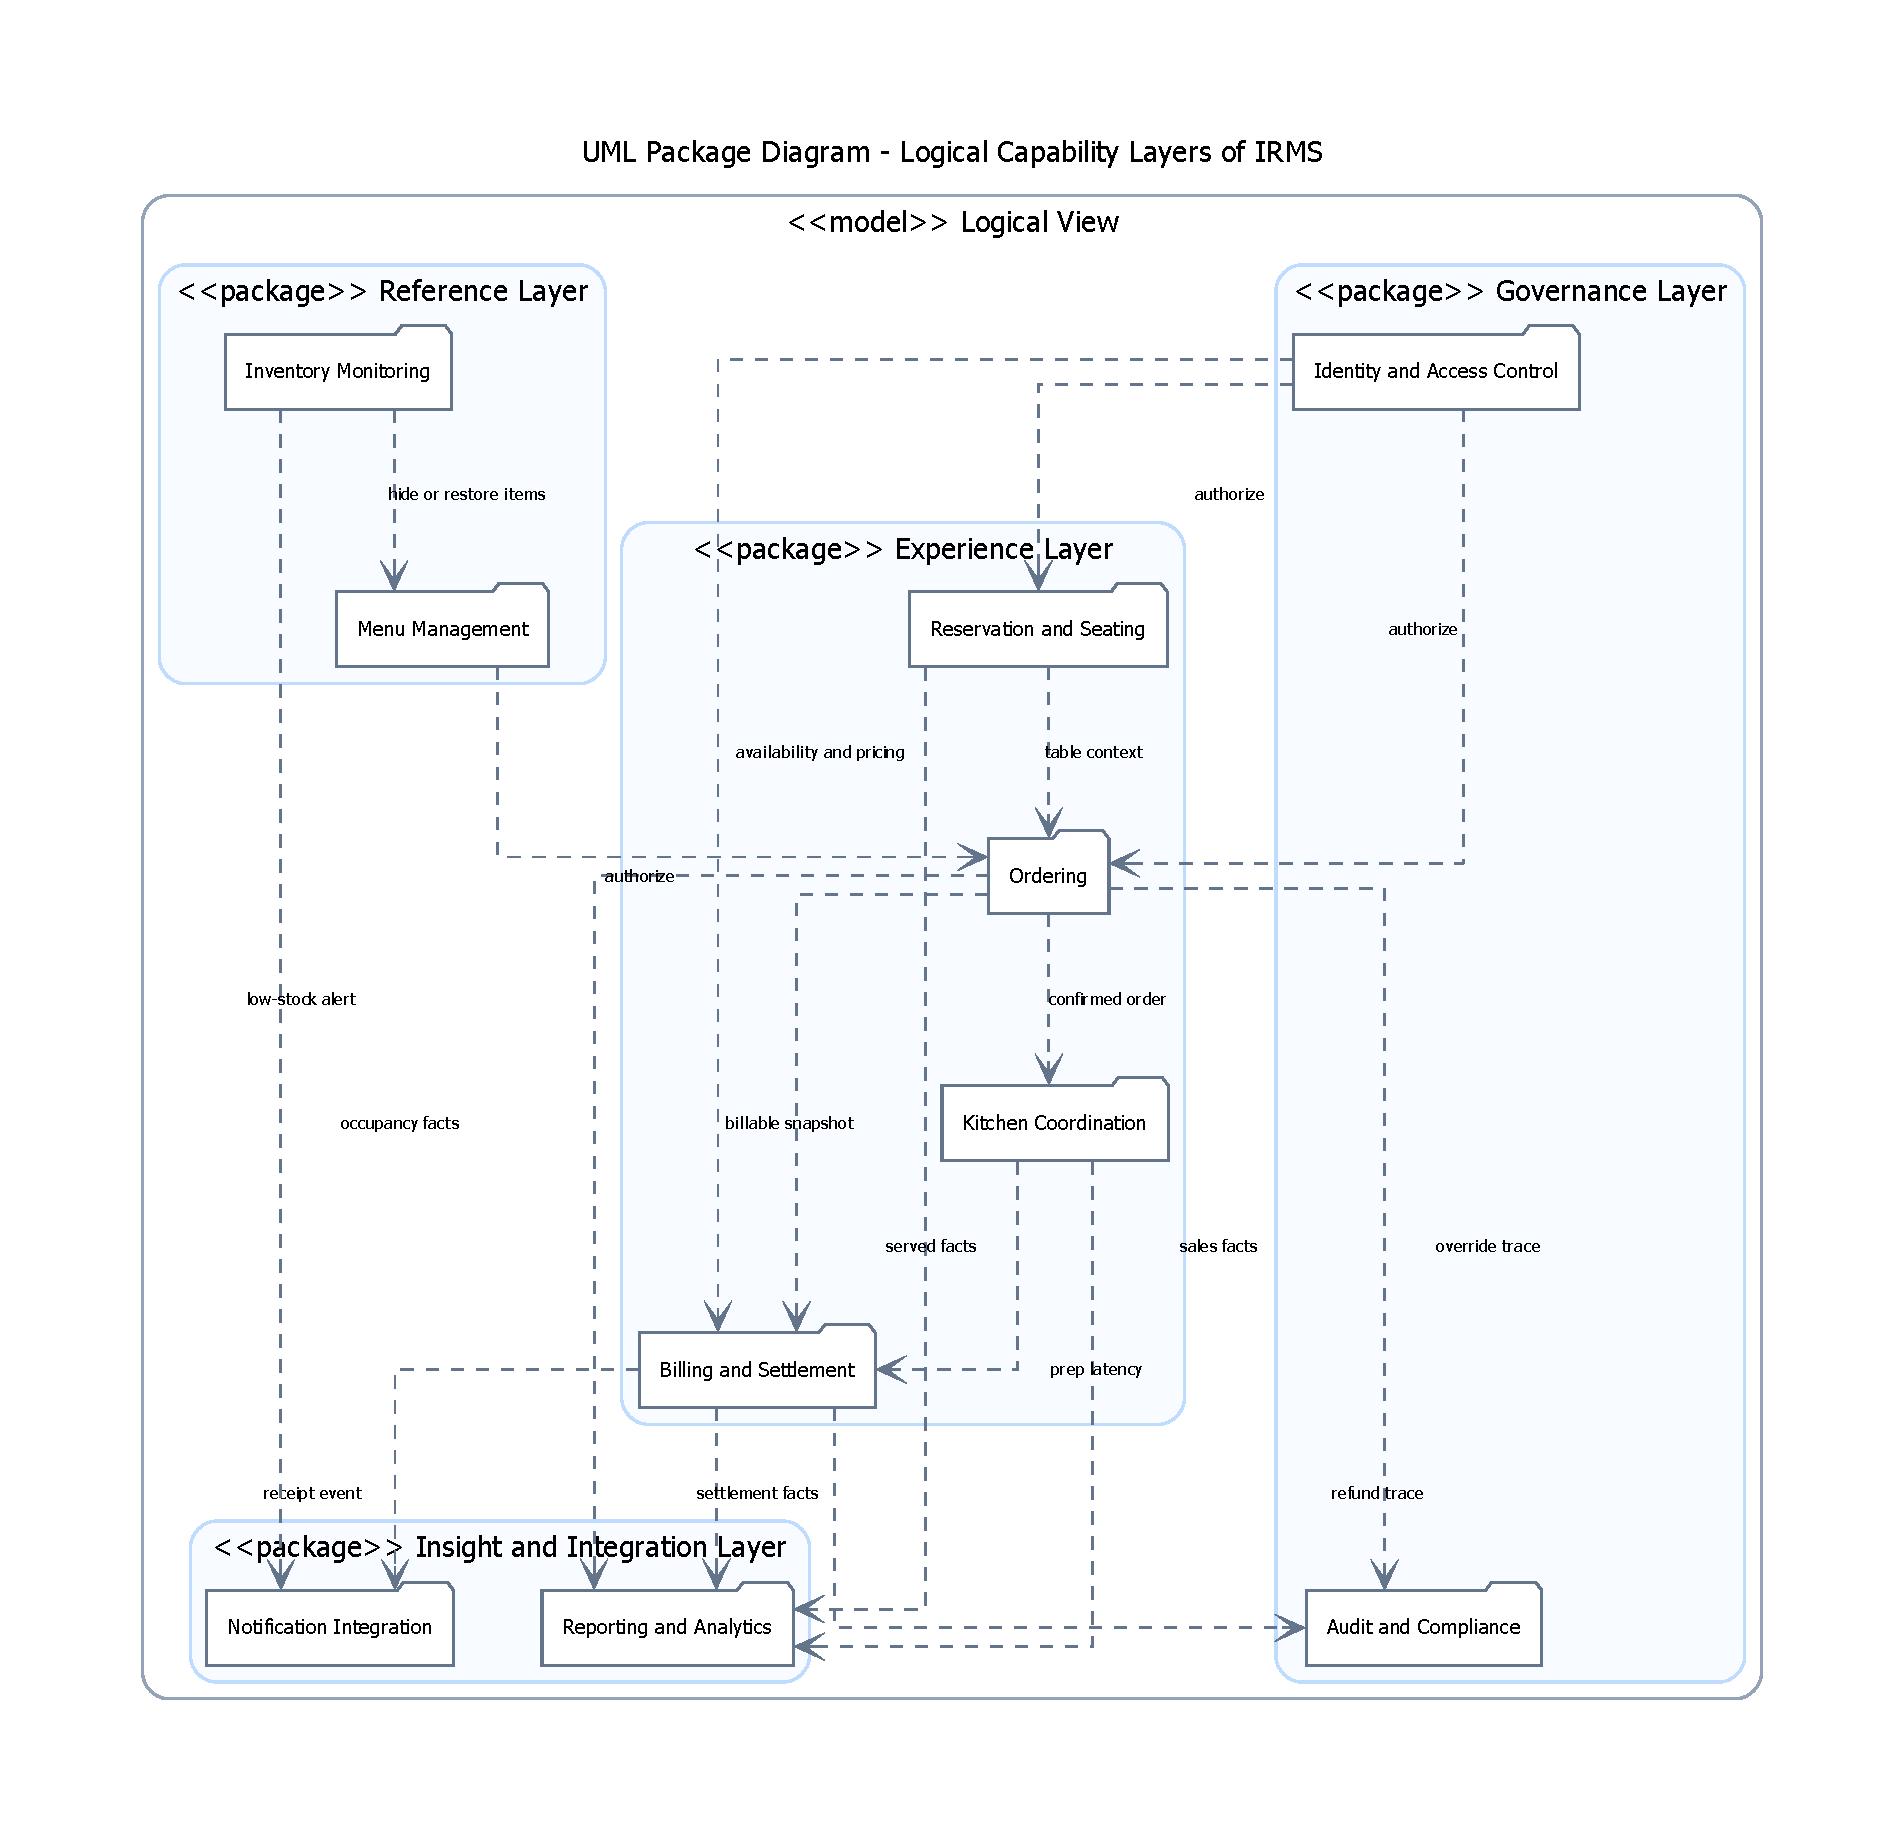
\includegraphics[width=\textwidth,height=0.82\textheight,keepaspectratio]{21_logical_view_overview_business_capability_layers.pdf}
}{
  \IfFileExists{21_logical_view_overview_business_capability_layers.png}{
    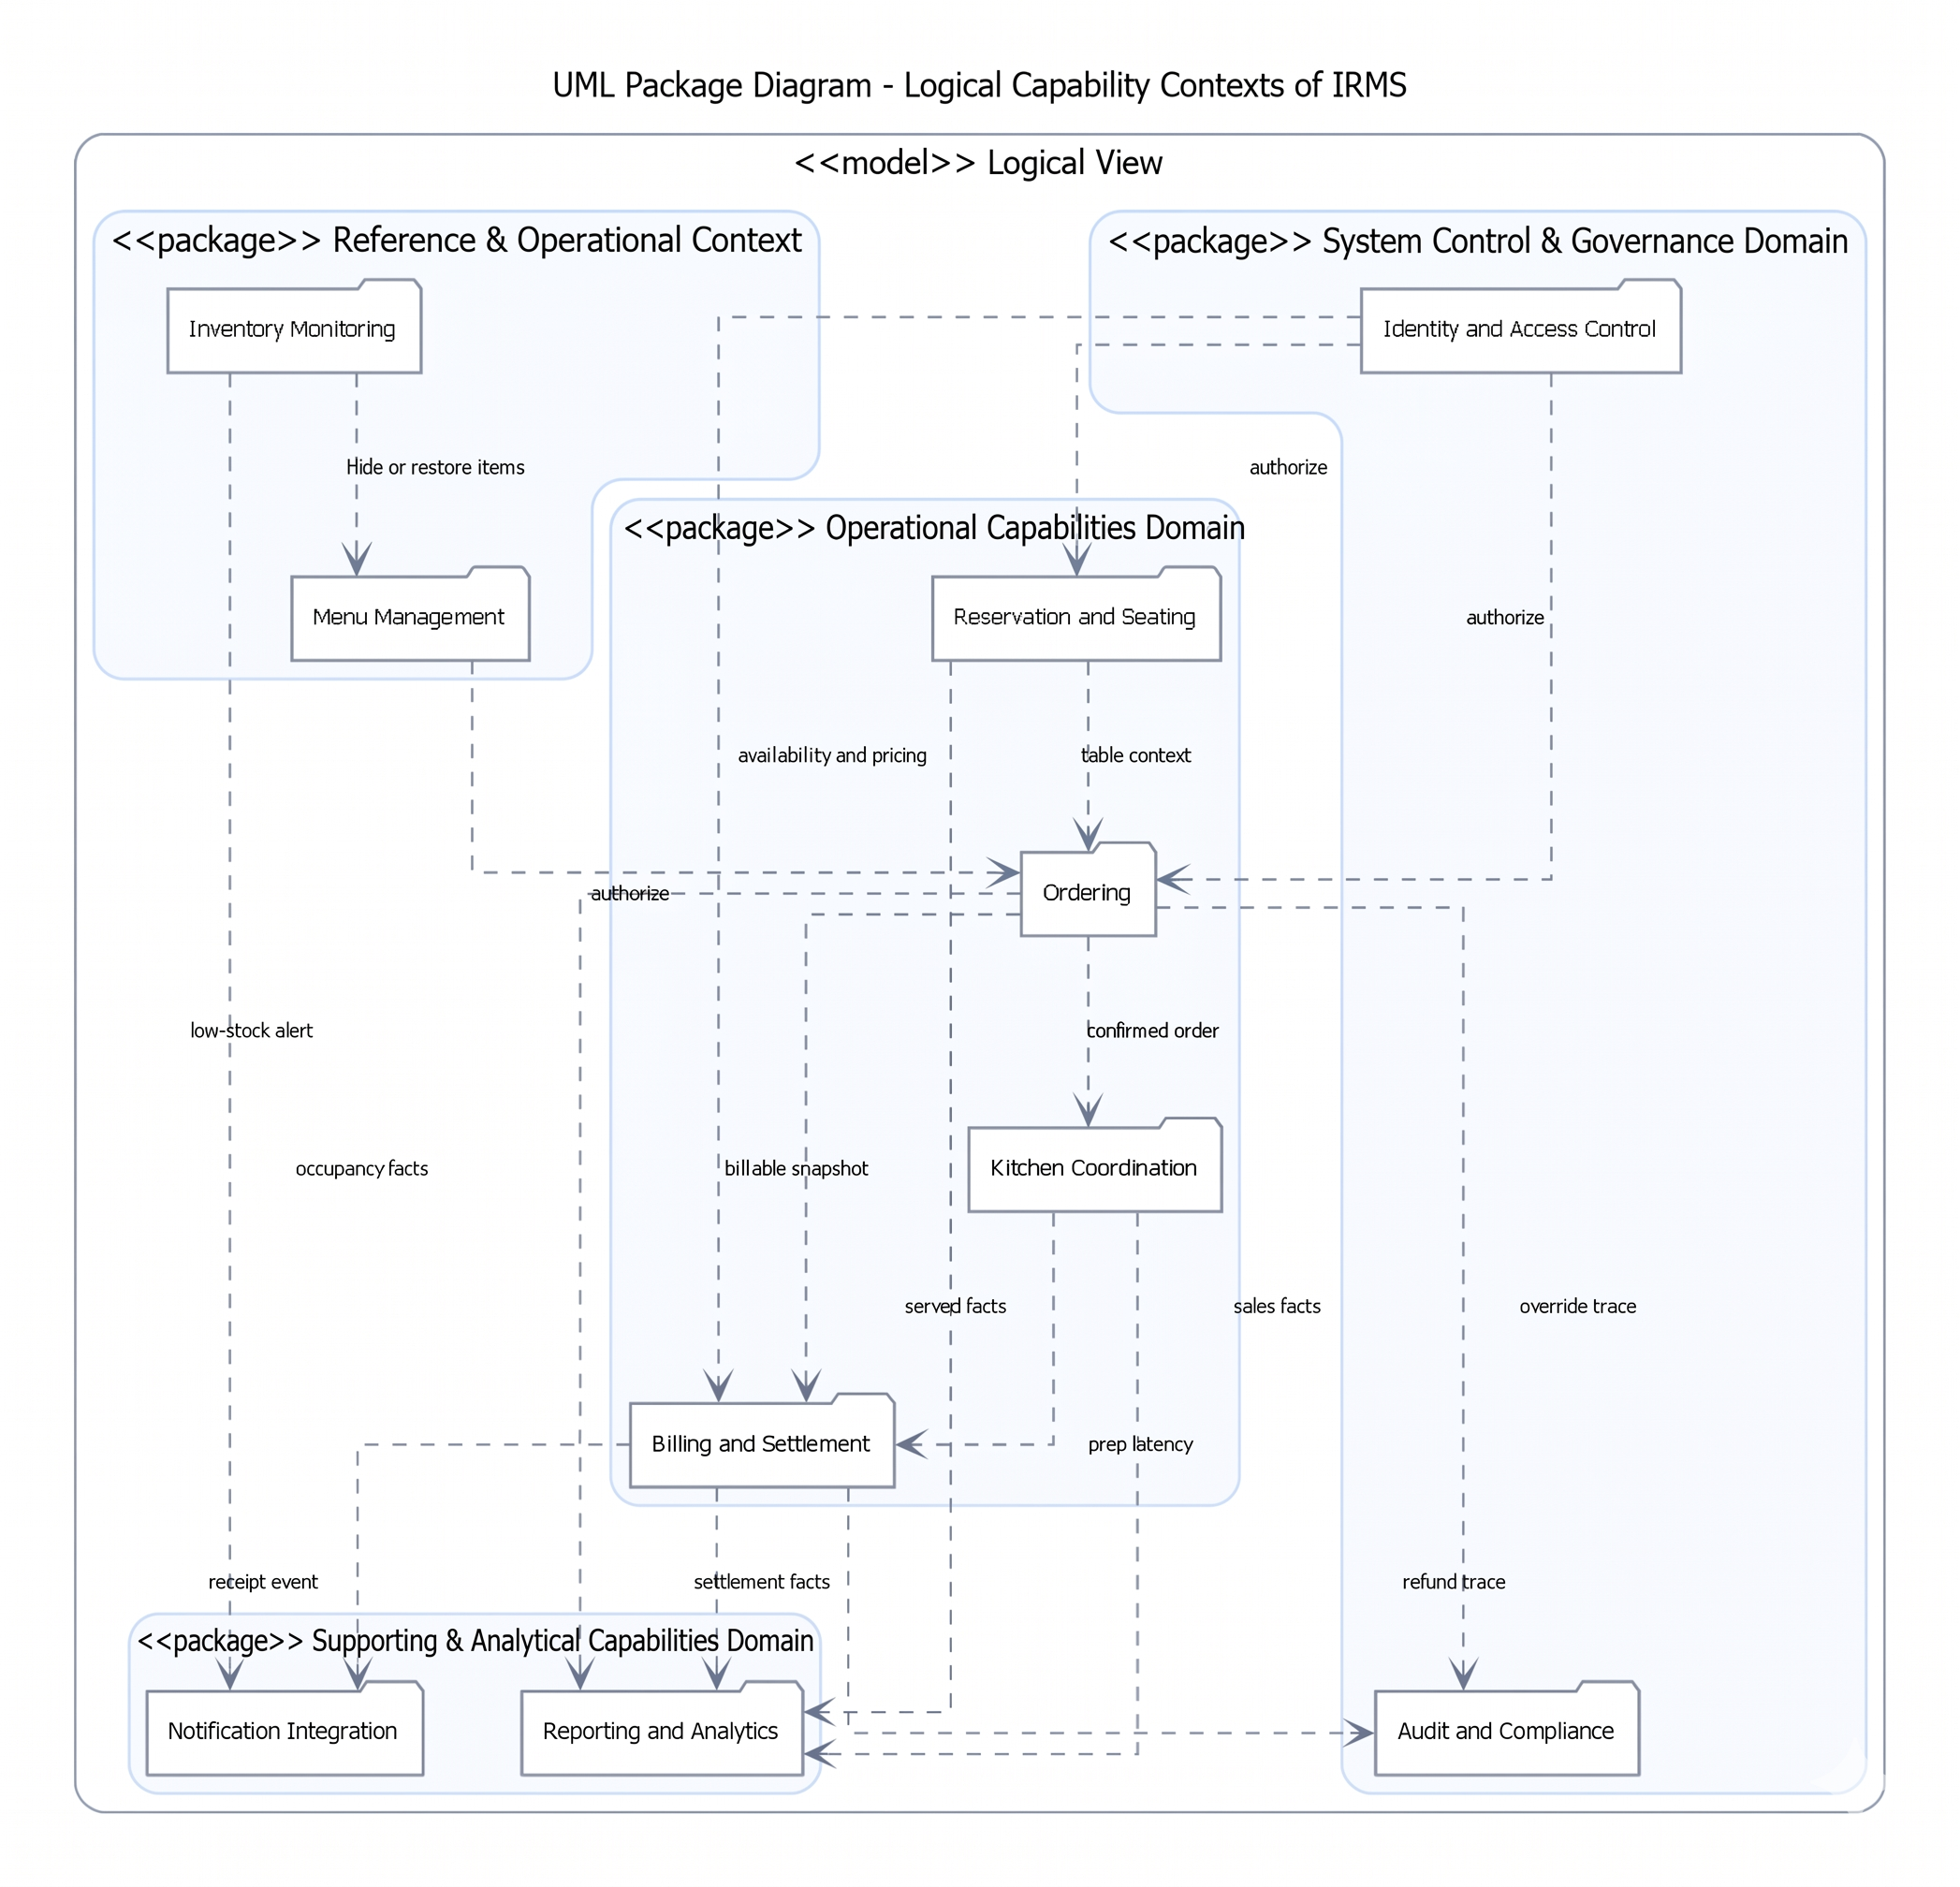
\includegraphics[width=\textwidth,height=0.82\textheight,keepaspectratio]{sodologictongquan.png}
  }{
    \fbox{\parbox{0.82\linewidth}{Thiếu file \textsf{21\_logical\_view\_overview\_business\_capability\_layers.(pdf/png)}.}}
  }
}
\caption{Sơ đồ năng lực nghiệp vụ hỗ trợ phân rã module của IRMS}
\label{fig:irms-logical-overview-supplement}
\end{figure}
Hình~\ref{fig:irms-logical-overview-supplement} trình bày sơ đồ năng lực nghiệp vụ của hệ thống IRMS dưới dạng UML Package, trong đó hệ thống được tổ chức dựa trên các năng lực nghiệp vụ (capabilities) thay vì theo giao diện người dùng hoặc cấu trúc kỹ thuật. Mục tiêu của sơ đồ hỗ trợ này là xác định các miền nghiệp vụ độc lập, đồng thời thể hiện mối quan hệ tương tác giữa chúng trước khi được ánh xạ sang các module và service trong các góc nhìn kiến trúc chính.

Trong kiến trúc IRMS, sơ đồ năng lực này được xây dựng theo hướng service-based architecture kết hợp với cơ chế event-driven interaction ở mức khái niệm. Mỗi package tương ứng với một miền năng lực có ranh giới rõ ràng. Sự tương tác giữa các miền được thể hiện thông qua hai cơ chế chính, bao gồm giao tiếp đồng bộ theo mô hình request/response trong luồng nghiệp vụ chính và giao tiếp bất đồng bộ thông qua domain events nhằm truyền tải thông tin vận hành mà không làm tăng mức độ phụ thuộc giữa các miền.

Từ cách tổ chức này, các năng lực nghiệp vụ trong hệ thống được phân nhóm theo vai trò trong kiến trúc tổng thể.

\textbf{Thứ nhất, nhóm năng lực tham chiếu và điều kiện vận hành} đóng vai trò cung cấp dữ liệu nền và đảm bảo điều kiện cho các luồng nghiệp vụ chính. \textit{Menu Management} chịu trách nhiệm quản lý thông tin món ăn, giá bán và trạng thái hiển thị, trong khi \textit{Inventory Monitoring} theo dõi tình trạng tồn kho và phát hiện các điều kiện thiếu hụt nguyên liệu. Nhóm này không trực tiếp tham gia xử lý giao dịch nhưng ảnh hưởng đến tính hợp lệ của dữ liệu trong toàn bộ hệ thống.

\textbf{Thứ hai, chuỗi năng lực cốt lõi} phản ánh toàn bộ vòng đời phục vụ trong nhà hàng. \textit{Reservation \& Seating} đảm nhiệm việc quản lý đặt bàn và phân bổ chỗ ngồi, tạo ngữ cảnh cho \textit{Ordering} trong quá trình tiếp nhận đơn hàng. Sau đó, \textit{Kitchen Coordination} tiếp nhận thông tin từ đơn hàng để điều phối quá trình chế biến món ăn, trong khi \textit{Billing \& Settlement} thực hiện thanh toán và kết thúc phiên phục vụ. Các năng lực trong chuỗi này có quan hệ phụ thuộc logic rõ ràng nhằm đảm bảo luồng nghiệp vụ được xử lý nhất quán.

\textbf{Thứ ba, nhóm năng lực hỗ trợ và phân tích} chịu trách nhiệm xử lý thông tin vận hành theo hướng bất đồng bộ. \textit{Notification Integration} tiếp nhận các sự kiện phát sinh để thực hiện thông báo, trong khi \textit{Reporting \& Analytics} tổng hợp dữ liệu từ nhiều miền nghiệp vụ nhằm phục vụ thống kê và phân tích. Việc tách nhóm này giúp giảm tải cho luồng xử lý chính và tăng khả năng mở rộng hệ thống.

\textbf{Thứ tư, nhóm năng lực kiểm soát hệ thống} đảm bảo các yêu cầu về bảo mật, phân quyền và truy vết. \textit{Identity \& Access Control} quản lý xác thực và phân quyền người dùng, trong khi \textit{Audit \& Compliance} ghi nhận lịch sử hoạt động để phục vụ kiểm toán và tuân thủ. Đây là các năng lực xuyên suốt toàn hệ thống nhưng không tham gia trực tiếp vào luồng nghiệp vụ chính.

\subsubsection{Tổng quan cho góc nhìn mô-đun}
\noindent
Góc nhìn mô-đun mô tả các đơn vị hiện thực chính của backend IRMS, cách chúng được tổ chức thành package, trách nhiệm của từng module và quan hệ phụ thuộc tĩnh giữa các module. Góc nhìn này cũng ghi nhận các cấu trúc dữ liệu dùng chung như \textsf{outbox\_events}, \textsf{processed\_events}, nhật ký kiểm toán và mô hình đọc báo cáo khi chúng ảnh hưởng đến nhiều module. Các cấu trúc dữ liệu này là nhóm bảng hoặc trách nhiệm lưu trữ logic trong cùng PostgreSQL, không phải các database vật lý riêng. Module View không mô tả tiến trình runtime hay luồng message khi hệ thống chạy; các nội dung đó thuộc Component-and-Connector View và Deployment View.

\begin{figure}[H]
\centering
\IfFileExists{22_module_view_overview_layered_dependencies.pdf}{
  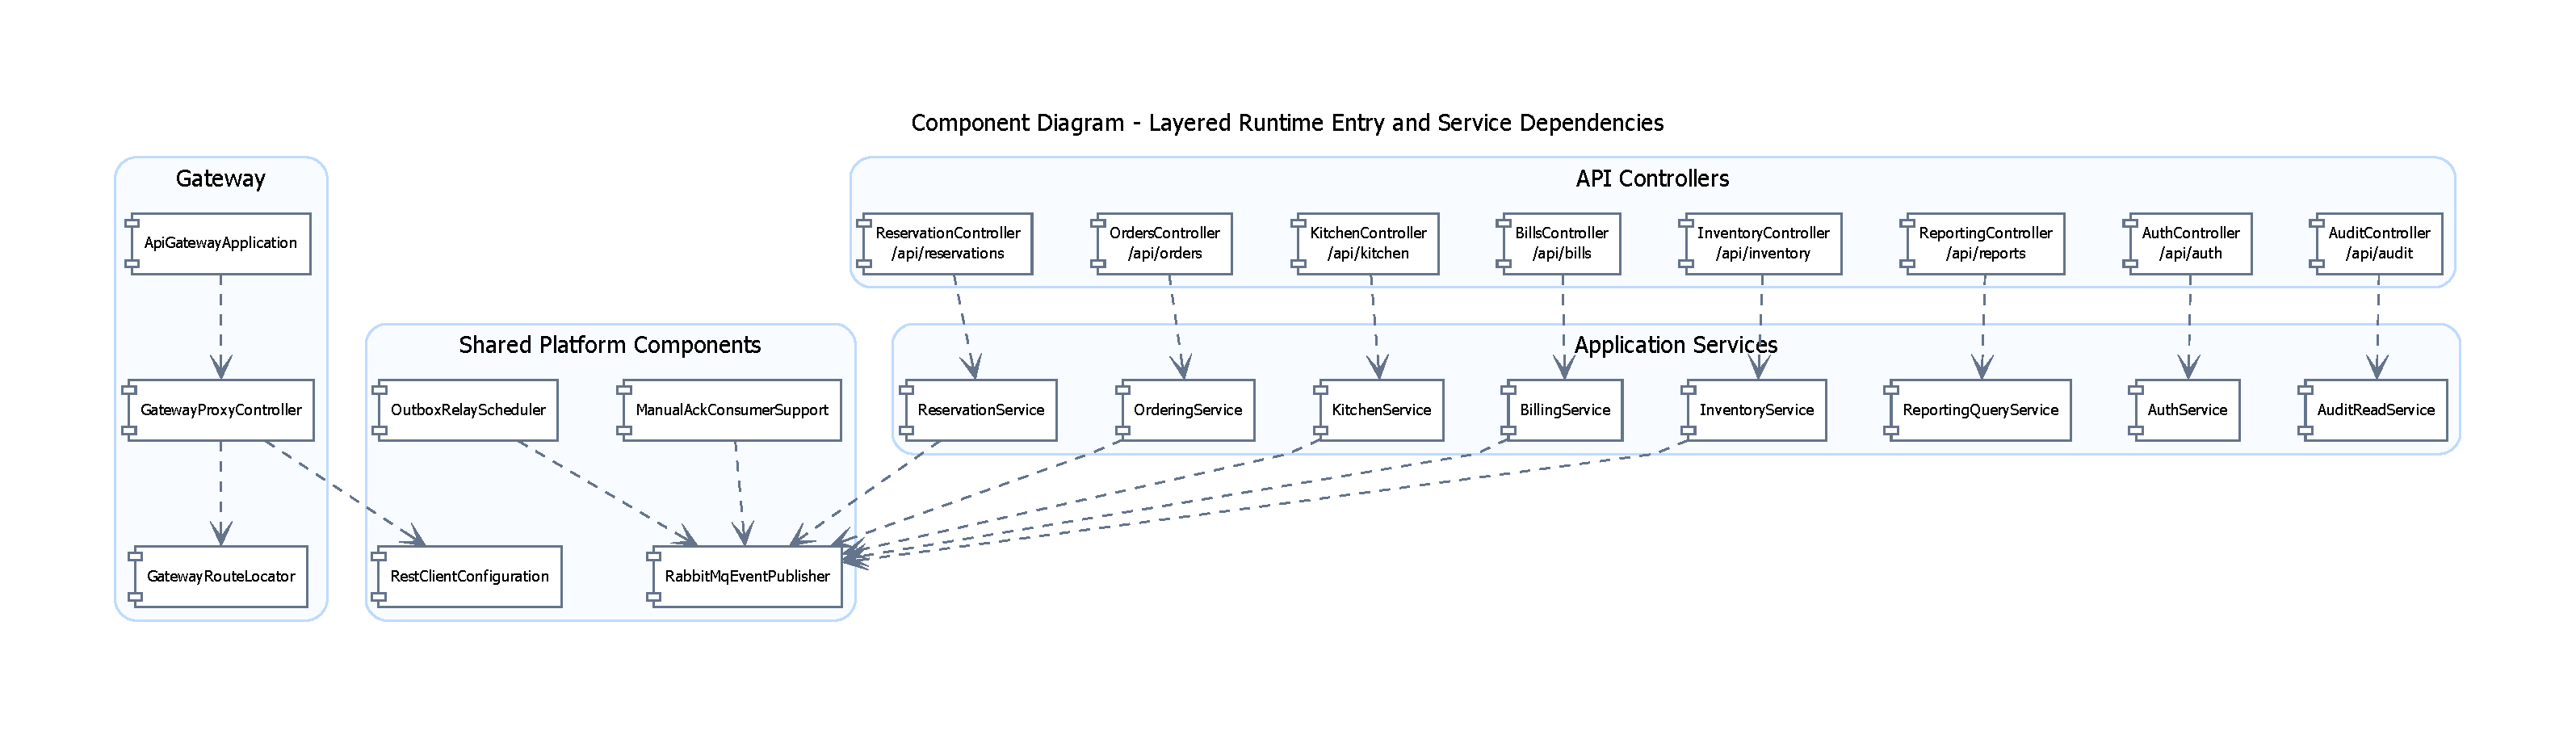
\includegraphics[width=\textwidth,height=0.82\textheight,keepaspectratio]{22_module_view_overview_layered_dependencies.pdf}
}{
  \IfFileExists{22_module_view_overview_layered_dependencies.png}{
    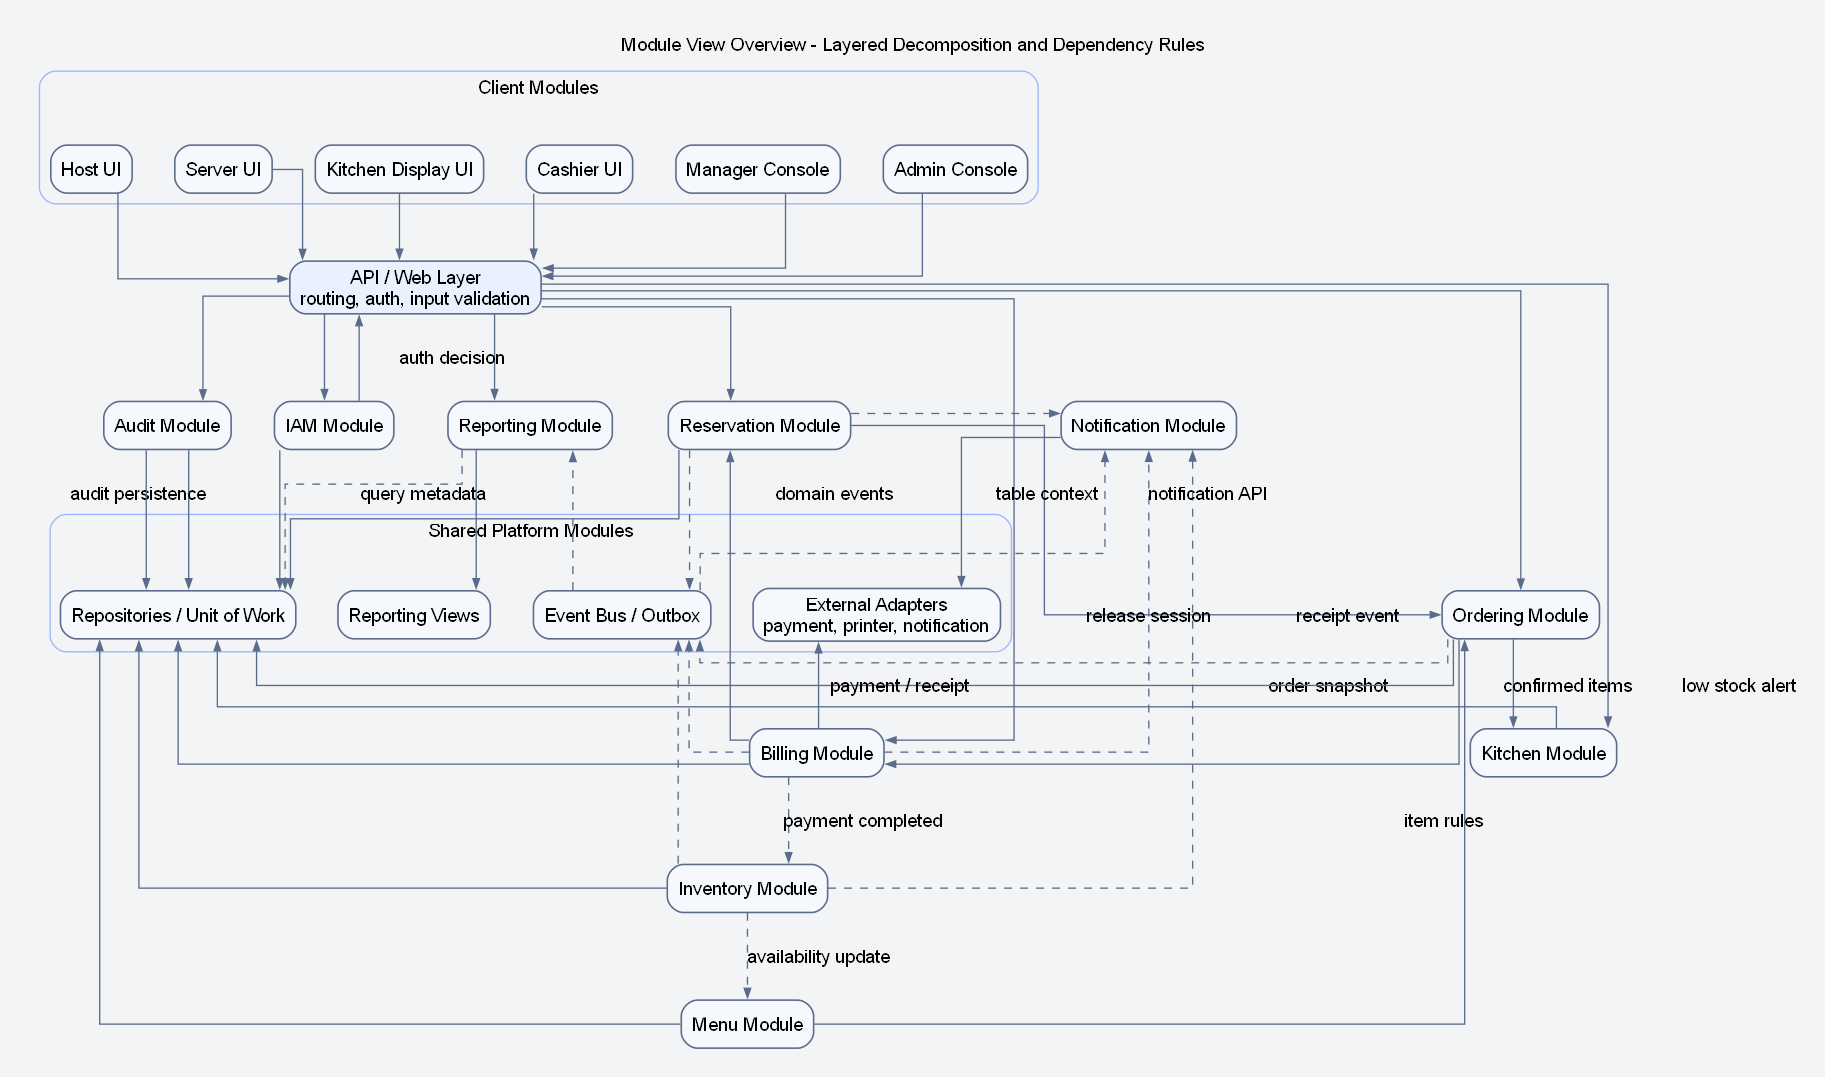
\includegraphics[width=\textwidth,height=0.82\textheight,keepaspectratio]{22_module_view_overview_layered_dependencies.png}
  }{
    \fbox{\parbox{0.82\linewidth}{Thiếu file \textsf{22\_module\_view\_overview\_layered\_dependencies.(pdf/png)}.}}
  }
}
\caption{Module View tổng quan theo lớp phụ thuộc của IRMS}
\label{fig:irms-module-overview-supplement}
\end{figure}


Hình~\ref{fig:irms-module-overview-supplement} thể hiện quy tắc phụ thuộc theo lớp bằng Module View, bám vào package và lớp hiện thực trong backend. 

\paragraph{Mô tả}
\begin{itemize}
  \item \textsf{GatewayProxyController} đi qua \textsf{GatewayRouteLocator} và \textsf{RestClientConfiguration} để định tuyến REST, không gọi trực tiếp vào dữ liệu nghiệp vụ.
  \item Các controller như \textsf{OrdersController}, \textsf{KitchenController} và \textsf{BillsController} phụ thuộc vào service ứng dụng tương ứng, đúng với cấu trúc package trong backend.
  \item Các thành phần hạ tầng dùng chung như \textsf{RabbitMqEventPublisher}, \textsf{RabbitMqOutboxRelay} và \textsf{ManualAckConsumerSupport} được đặt riêng để xử lý sự kiện và bộ xử lý sự kiện nền.
\end{itemize}


\paragraph{Catalog mô-đun và ánh xạ hiện thực.}
Bảng~\ref{tab:irms-module-catalog} thể hiện giới mô-đun theo package trong backend. Các hình Module View ở phần này mô tả tổ chức tĩnh và hướng phụ thuộc giữa package, còn các sơ đồ Component-and-Connector phía sau mới mô tả cộng tác runtime.

\begin{table}[H]
\centering
\footnotesize
\renewcommand{\arraystretch}{1.18}
\caption{Catalog mô-đun backend IRMS}
\label{tab:irms-module-catalog}
\begin{tabularx}{\textwidth}{>{\raggedright\arraybackslash}p{0.17\linewidth} >{\raggedright\arraybackslash}X >{\raggedright\arraybackslash}p{0.32\linewidth}}
\toprule
\textbf{Module} & \textbf{Trách nhiệm} \\
\midrule
\textsf{Gateway} & Điểm vào REST, chuẩn hóa đường \textsf{/api/**} và định tuyến đến service nghiệp vụ theo cấu hình.\\
\textsf{Runtime / Bootstrap} & Chứa các entrypoint Spring Boot và profile khởi động từng runtime trong Docker.  \\
\textsf{Reservation} & Đặt bàn, danh sách chờ, sơ đồ bàn, check-in và phiên phục vụ. \\
\textsf{Ordering} & Thực đơn, tạo/xác nhận order, tùy biến món, combo, snapshot giá và gửi bếp. \\
\textsf{Kitchen} & Điều phối phiếu bếp, trạng thái món, deadline, ưu tiên và workflow chế biến. \\
\textsf{Billing} & Lập hóa đơn, tách hóa đơn, thanh toán, hoàn tiền, biên nhận và settlement. \\
\textsf{Inventory} & Theo dõi tồn kho, tiêu hao nguyên liệu, cảnh báo mức tồn thấp và đề xuất nhập hàng.  \\
\textsf{Notification} & Ghi nhận yêu cầu thông báo và chọn adapter kênh gửi nội bộ. \\
\textsf{Reporting} & Dashboard, báo cáo vận hành và các bảng mô hình đọc/projection.  \\
\textsf{Identity/Audit} & Xác thực, vai trò, quyền, session, policy và nhật ký kiểm toán.  \\
\textsf{Common Platform} & Hạ tầng dùng chung: security/context, lỗi chuẩn, workflow, outbox, RabbitMQ và consumer support. \\
\textsf{PDF / Receipt Adapter} & Render/phát hành biên nhận qua adapter nội bộ, không mô tả máy in vật lý hay nhà cung cấp ngoài. \\
\bottomrule
\end{tabularx}
\end{table}

\begin{table}[H]
\centering
\footnotesize
\renewcommand{\arraystretch}{1.18}
\caption{Interface và phụ thuộc chính của các mô-đun}
\label{tab:irms-module-contracts}
\begin{tabularx}{\textwidth}{>{\raggedright\arraybackslash}p{0.16\linewidth} >{\raggedright\arraybackslash}X >{\raggedright\arraybackslash}X}
\toprule
\textbf{Module} & \textbf{Class/interface tiêu biểu và contract nhìn thấy} & \textbf{Phụ thuộc và dữ liệu dùng chung} \\
\midrule
\textsf{Gateway} & \textsf{GatewayProxyController}; \textsf{GatewayRouteLocator}; contract HTTP proxy cho route \textsf{/api/**}. & Dùng cấu hình URL service và common error/context; không gọi trực tiếp dữ liệu nghiệp vụ. \\
\textsf{Runtime / Bootstrap} & \textsf{ApiGatewayApplication}, \textsf{OrderingServiceApplication}, \textsf{KitchenServiceApplication}, \textsf{BillingServiceApplication}, \textsf{ReservationServiceApplication}, \textsf{InventoryServiceApplication}, \textsf{NotificationServiceApplication}, \textsf{ReportingServiceApplication}, \textsf{IdentityAuditServiceApplication}. & Chọn service boundary bằng profile, port và biến môi trường trong \texttt{docker-compose.yml}. \\
\textsf{Reservation} & \textsf{ReservationService}, \textsf{ReservationCheckInService}, \textsf{ReservationTableAssignmentService}. & Dùng identity/common để kiểm soát thao tác; ghi bảng reservation/table session và event qua outbox nếu phát sinh. \\
\textsf{Ordering} & \textsf{OrdersService}, \textsf{OrderMenuSelectionService}, \textsf{ComboPricingPolicy}, \textsf{OrderStatusPolicy}. & Dùng reservation/table-session context, kitchen integration client và common outbox/messaging. \\
\textsf{Kitchen} & \textsf{KitchenService}, \textsf{KitchenOrderRoutingService}, \textsf{KitchenWorkflowMediator}, \textsf{KitchenTicketTransitionPolicy}, \textsf{KitchenTicketItemRepositoryPort}. & Nhận order/kitchen events; dùng \textsf{ManualAckConsumerSupport} và \textsf{processed\_events} cho bộ xử lý sự kiện nền. \\
\textsf{Billing} & \textsf{BillingService}, \textsf{BillingPaymentService}, \textsf{BillingReceiptService}, \textsf{PaymentGateway}, \textsf{ReceiptDeliveryAdapter}, \textsf{BillSplitStrategy}. & Dùng billable snapshot từ ordering, adapter thanh toán/biên nhận và \textsf{DomainEventPublisher}. \\
\textsf{Inventory} & \textsf{InventoryService}, \textsf{InventoryStockChangedConsumer}, \textsf{LowStockSeverityPolicy}, \textsf{ReorderRecommendationStrategy}. & Tiêu thụ event qua RabbitMQ/manual ack; ghi inventory tables và có thể phát cảnh báo tồn thấp. \\
\textsf{Notification} & \textsf{NotificationService}, \textsf{NotificationRequestedConsumer}, \textsf{NotificationChannelAdapter} và các adapter email/SMS/in-app/print. & Nhận yêu cầu thông báo từ sự kiện; kênh gửi được che sau adapter biên nội bộ. \\
\textsf{Reporting} & \textsf{ReportingQueryService}, \textsf{ReportingProjectionConsumer}, các projection/materializer. & Dùng domain events, \textsf{processed\_events} và các bảng \texttt{reporting\_\char`*\_projection}. \\
\textsf{Identity/Audit} & \textsf{AuthService}, \textsf{AuditService}, \textsf{IdentityRepository}, \textsf{IdentityPolicyRepository}, \textsf{AuditRecordingRequestedConsumer}. & Duy trì user/session/role/policy và \textsf{audit\_logs}; các module bảo vệ thao tác dùng chính sách identity. \\
\textsf{Common Platform} & \textsf{TransactionalOutboxPublisher}, \textsf{RabbitMqOutboxRelay}, \textsf{RabbitMqEventPublisher}, \textsf{ManualAckConsumerSupport}, \textsf{ApiEnvelope}. & Crosscutting package cho \textsf{outbox\_events}, \textsf{processed\_events}, envelope/correlation và lỗi chuẩn. \\
\bottomrule
\end{tabularx}
\end{table}

\begin{table}[H]
\centering
\scriptsize
\renewcommand{\arraystretch}{1.15}
\setlength{\tabcolsep}{2pt}
\caption{Các loại quan hệ dùng trong Module View}
\label{tab:irms-module-relation-types}
\begin{tabularx}{\textwidth}{>{\raggedright\arraybackslash}p{0.18\linewidth} >{\raggedright\arraybackslash}X >{\raggedright\arraybackslash}p{0.34\linewidth}}
\toprule
\textbf{Relation type} & \textbf{Ý nghĩa trong Module View} & \textbf{Ví dụ trong IRMS} \\
\midrule
\textsf{is-part-of} & Module/package con thuộc một package lớn hơn. & \textsf{ordering.api}, \textsf{ordering.application}, \textsf{ordering.domain}, \textsf{ordering.infrastructure} thuộc \textsf{SA.irms.ordering}. \\
\textsf{uses / depends-on} & Phụ thuộc source-level qua import, constructor, method call, config hoặc bean wiring. & \textsf{OrdersController} phụ thuộc \textsf{OrdersService}; \textsf{BillingPaymentService} phụ thuộc \textsf{PaymentGateway}. \\
\textsf{allowed-to-use} & Quy tắc tầng được phép dùng tầng thấp hơn hoặc package dùng chung. & \textsf{*.api} dùng \textsf{*.application}; \textsf{*.application} dùng \textsf{*.domain} và port/interface. \\
\textsf{data dependency} & Module đọc/ghi hoặc bị ảnh hưởng bởi cấu trúc dữ liệu dùng chung. & \textsf{RabbitMqOutboxRelay} dùng \textsf{outbox\_events}; bộ xử lý sự kiện nền dùng \textsf{processed\_events}. \\
\textsf{crosscuts} & Package dùng chung hỗ trợ nhiều module nghiệp vụ. & \textsf{SA.irms.common} cung cấp security/context, outbox, messaging, workflow và lỗi chuẩn. \\
\textsf{is-a} & Quan hệ kế thừa hoặc hiện thực interface ở mức class/interface. & \textsf{CashPaymentGateway} hiện thực \textsf{PaymentGateway}; notification adapters hiện thực \textsf{NotificationChannelAdapter}. \\
\bottomrule
\end{tabularx}
\end{table}

\begin{table}[H]
\centering
\footnotesize
\renewcommand{\arraystretch}{1.15}
\caption{Cấu trúc dữ liệu dùng chung trong Module View}
\label{tab:irms-global-data-structures}
\begingroup
\small
\setlength{\tabcolsep}{3pt}
\renewcommand{\arraystretch}{1.18}

\begin{tabularx}{\textwidth}{@{}
  >{\raggedright\arraybackslash}p{0.18\textwidth}
  >{\raggedright\arraybackslash}p{0.22\textwidth}
  >{\raggedright\arraybackslash}X
  >{\raggedright\arraybackslash}p{0.23\textwidth}
@{}}
\toprule
\textbf{Cấu trúc} &
\textbf{Module duy trì} &
\textbf{Vai trò trong góc nhìn mô-đun} &
\textbf{Thành phần liên quan} \\
\midrule

\textsf{outbox\_events} &
\textsf{SA.irms.common.outbox} và các module phát event. &
Bảng dùng chung để ghi sự kiện cần phát bất đồng bộ trước khi chuyển sang \textsf{RabbitMQ}. &
\begin{tabular}[t]{@{}l@{}}
\textsf{TransactionalOutbox}\\
\textsf{Publisher};\\
\textsf{RabbitMqOutboxRelay}.
\end{tabular} \\

\textsf{processed\_events} &
\textsf{SA.irms.common.messaging}. &
Bảng ghi nhận sự kiện đã xử lý, giúp tránh xử lý lặp trong các luồng nền. &
\begin{tabular}[t]{@{}l@{}}
\textsf{ManualAckConsumer}\\
\textsf{Support}.
\end{tabular} \\

\begin{tabular}[t]{@{}l@{}}
\texttt{reporting\_\char`*\_}\\
\texttt{projection}
\end{tabular} &
\textsf{SA.irms.reporting}. &
Mô hình đọc cho dashboard và báo cáo, được cập nhật qua các thành phần tổng hợp dữ liệu. &
\begin{tabular}[t]{@{}l@{}}
\textsf{ReportingProjection}\\
\textsf{Consumer};\\
\textsf{ReportingQueryService}.
\end{tabular} \\

\begin{tabular}[t]{@{}l@{}}
\textsf{audit\_logs},\\
\textsf{audit\_details}
\end{tabular} &
\textsf{SA.irms.identity}. &
Dữ liệu kiểm toán cho thao tác nhạy cảm và truy vết vận hành. &
\begin{tabular}[t]{@{}l@{}}
\textsf{AuditService};\\
\textsf{AuditRecording}\\
\textsf{RequestedConsumer}.
\end{tabular} \\

\begin{tabular}[t]{@{}l@{}}
\textsf{identity/session/}\\
\textsf{policy data}
\end{tabular} &
\textsf{SA.irms.identity}. &
Dữ liệu xác thực, phân quyền, session và chính sách được nhiều module tham chiếu. &
\begin{tabular}[t]{@{}l@{}}
\textsf{AuthService};\\
\textsf{IdentityPolicy}\\
\textsf{Repository}.
\end{tabular} \\

\bottomrule
\end{tabularx}
\endgroup
\end{table}

\subsubsection{Tổng quan cho góc nhìn thành phần và kết nối}

Góc nhìn thành phần và kết nối mô tả các thành phần có mặt ở runtime và cách chúng giao tiếp qua REST, JDBC, AMQP, outbox và các adapter biên. Khác với Module View, góc nhìn này không chỉ mô tả package tĩnh mà làm rõ component nào cung cấp interface, component nào yêu cầu interface, port nào nằm ở biên subsystem và connector nào lắp ghép các interface đó. Trong IRMS, trọng tâm của C\&C View là tuyến đi từ frontend/API Gateway vào controller/service nghiệp vụ, tuyến ghi dữ liệu vào PostgreSQL vật lý duy nhất, và tuyến event-driven đi qua outbox, RabbitMQ, bộ xử lý sự kiện nền, read model, notification và audit.

Phần chi tiết của Component-and-Connector View được trình bày ở Mục~\ref{sec:main-components} và các hình thành phần bên dưới. Các hình này cần được đọc như sơ đồ runtime collaboration có component, port/interface và connector, không phải package diagram hay class diagram.

\subsubsection{Tổng quan cho góc nhìn phân bổ}
\begin{figure}[H]
\centering
\IfFileExists{23_allocation_view_overview_software_to_runtime_mapping.pdf}{
  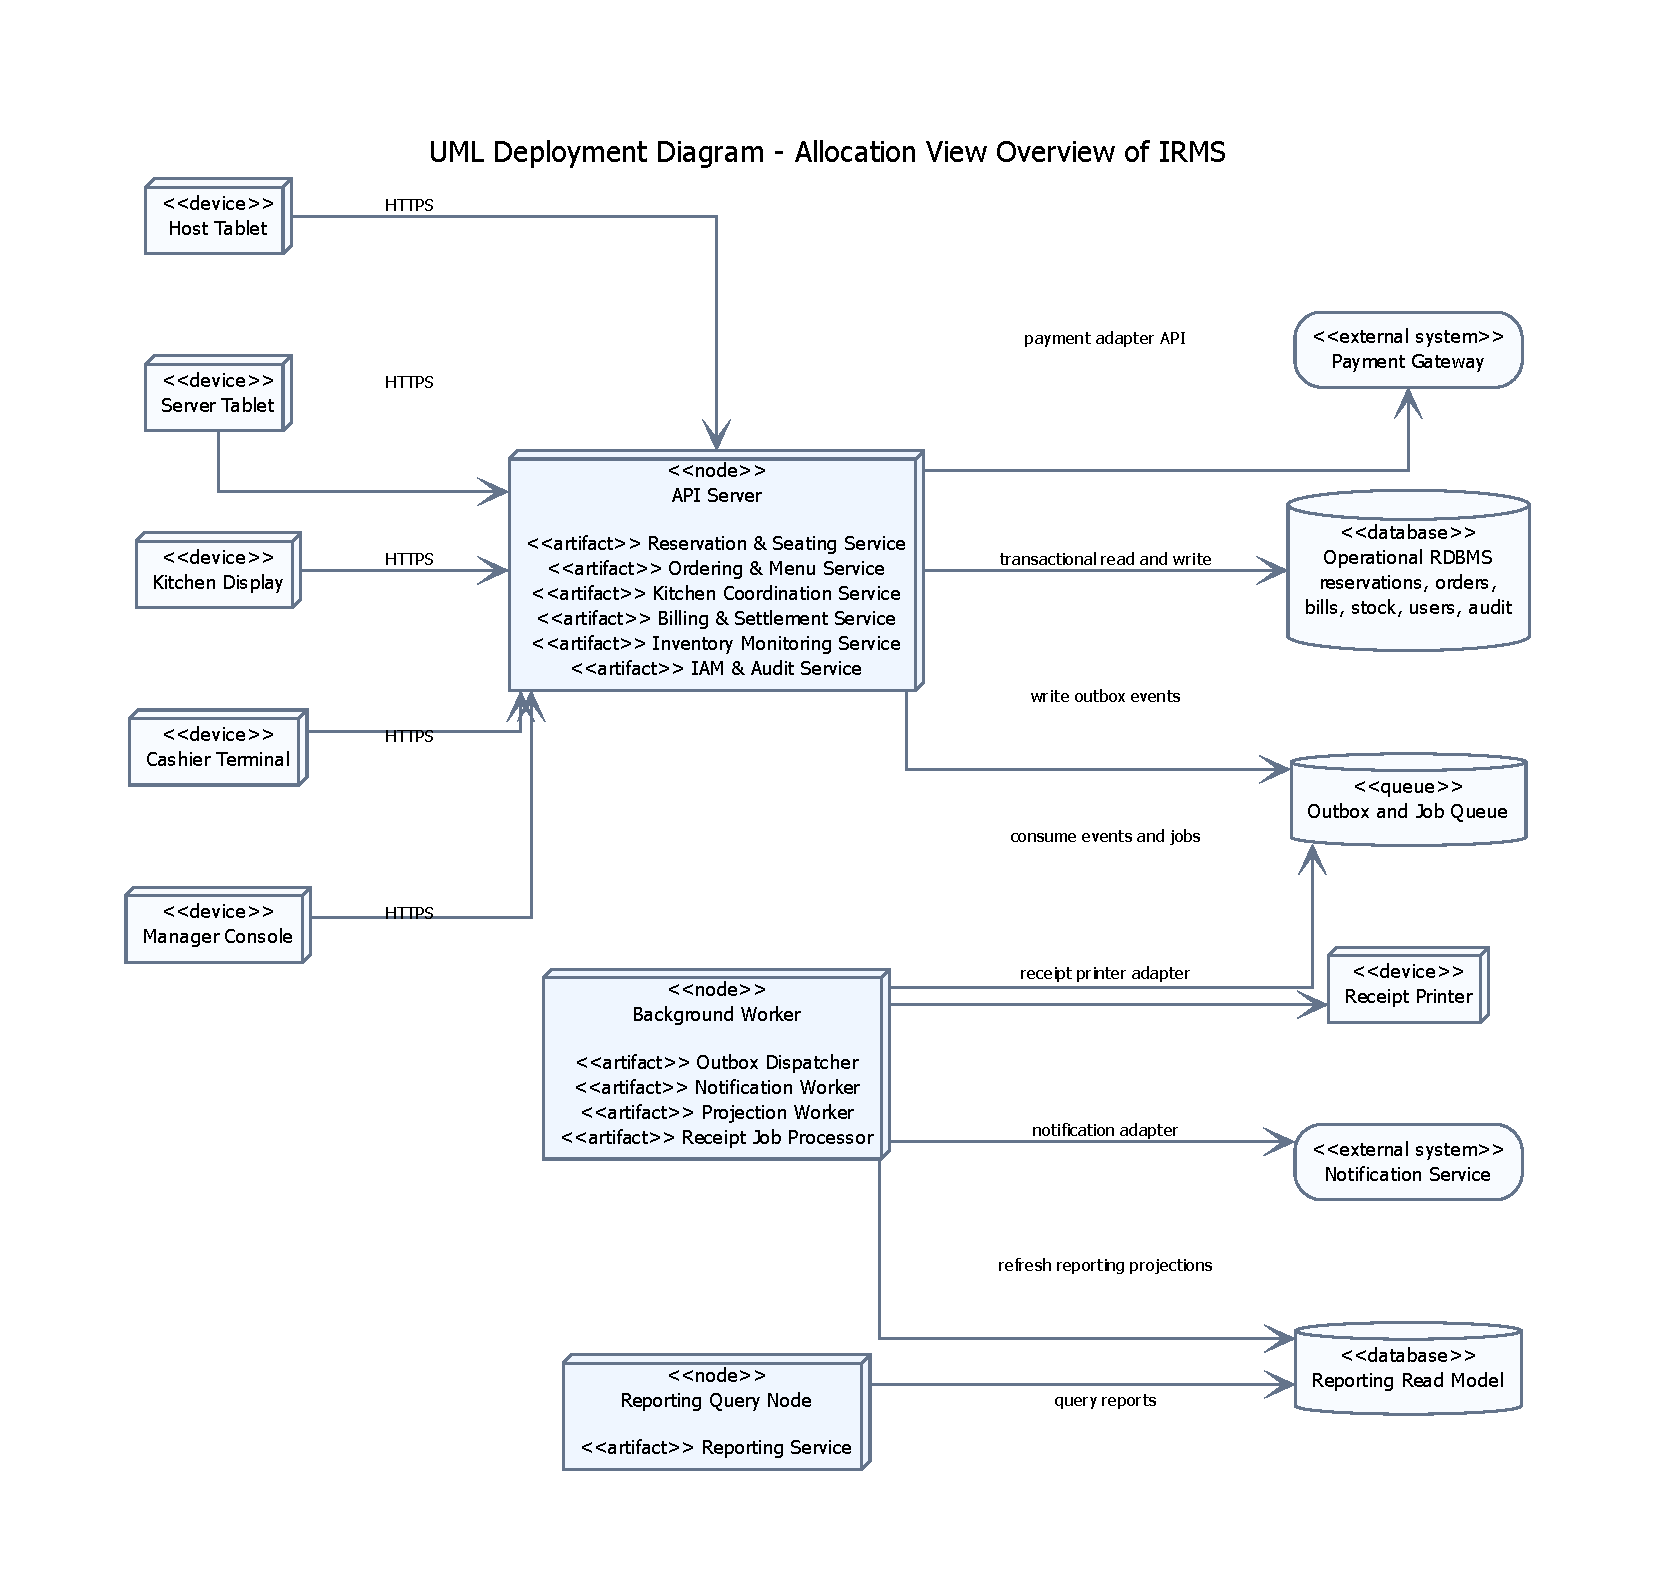
\includegraphics[width=\textwidth,height=0.84\textheight,keepaspectratio]{23_allocation_view_overview_software_to_runtime_mapping.pdf}
}{
  \IfFileExists{23_allocation_view_overview_software_to_runtime_mapping.png}{
    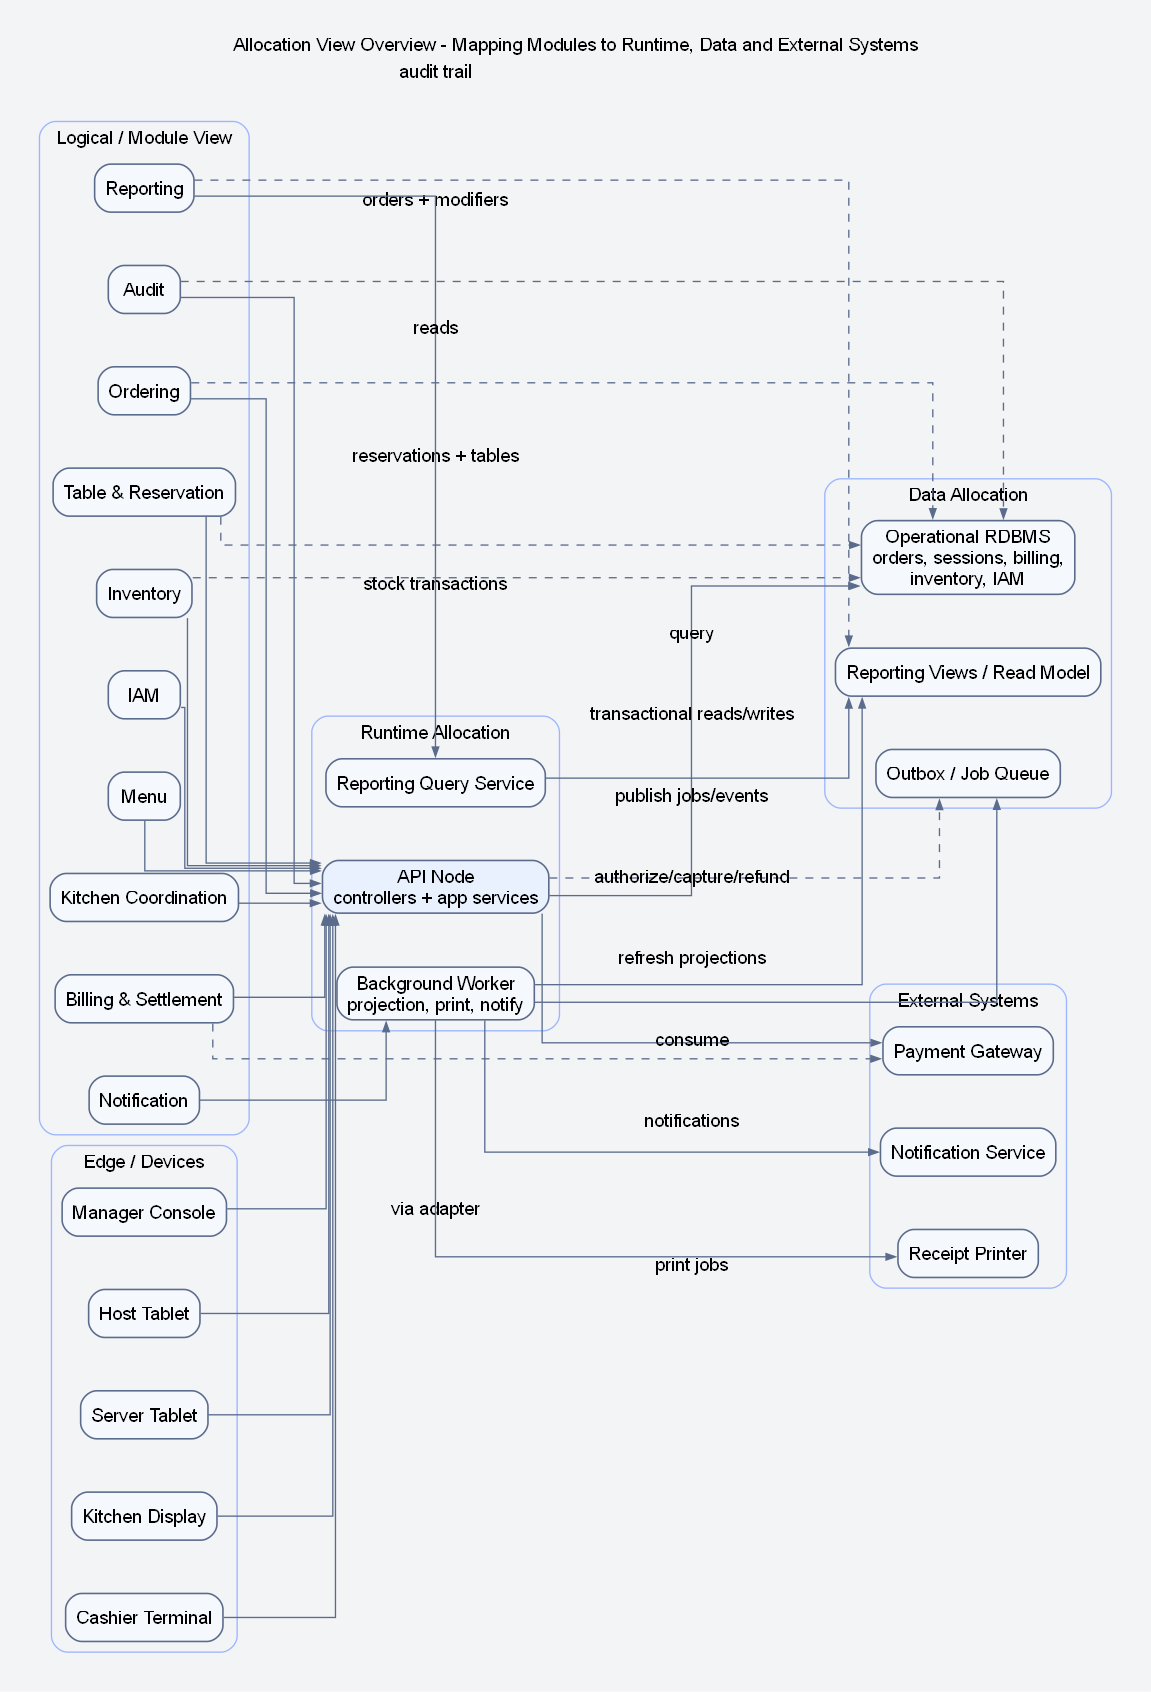
\includegraphics[width=\textwidth,height=0.84\textheight,keepaspectratio]{23_allocation_view_overview_software_to_runtime_mapping.png}
  }{
    \fbox{\parbox{0.82\linewidth}{Thiếu file \textsf{23\_allocation\_view\_overview\_software\_to\_runtime\_mapping.(pdf/png)}.}}
  }
}
\caption{Sơ đồ tổng quan cho góc nhìn phân bổ của IRMS}
\label{fig:irms-allocation-overview}
\end{figure}

\paragraph{Mô tả:}
\begin{itemize}
  \item \textbf{Lớp biên và thiết bị}: là nơi phát sinh thao tác nghiệp vụ thực tế như máy của lễ tân, máy của phục vụ, màn hình bếp, máy thu ngân và màn hình quản lý.
  \item \textbf{Lớp thực thi}: gồm \textsf{frontend container}, \textsf{api-gateway container}, nhóm container service Spring Boot và \textsf{irms-migration container}; đây là nơi các năng lực được hiện thực thành tiến trình hoặc vùng thực thi cụ thể.
  \item \textbf{Lớp dữ liệu và sự kiện}: gồm \textsf{PostgreSQL container}, \textsf{RabbitMQ container}, \textsf{outbox\_events}, \textsf{processed\_events} và các bảng hoặc view báo cáo; chúng tách dữ liệu giao dịch, dữ liệu đọc tổng hợp và hàng đợi sự kiện.
  \item \textbf{Lớp hệ thống ngoài}: hình này không vẽ hệ thống ngoài độc lập cho thanh toán, thông báo hoặc máy in vật lý; các năng lực đó được đặt sau adapter biên nội bộ trong phạm vi hiện tại.
\end{itemize}


\subsection{Đặc trưng kiến trúc}
Những \emph{đặc trưng kiến trúc} quan trọng là:
\begin{enumerate}
  \item \textbf{Khả năng đáp ứng}: màn hình gọi món, màn hình bếp và màn hình thu ngân phải phản hồi nhanh để không làm chậm tuyến phục vụ trực tiếp với khách.
  \item \textbf{Độ tin cậy}: đơn gọi món, thanh toán, hoàn tiền và cập nhật trạng thái bàn là các luồng không được mất dữ liệu hoặc xử lý lặp sai lệch.
  \item \textbf{Khả năng mở rộng}: điểm nóng thường dồn vào giờ cao điểm và tập trung ở các miền \textsf{Ordering}, \textsf{Kitchen Coordination} và \textsf{Billing} thay vì toàn hệ thống.
  \item \textbf{Bảo mật và khả năng kiểm toán}: mọi thao tác nhạy cảm phải được kiểm soát bằng quyền và truy vết lại được về sau.
  \item \textbf{Khả năng quan sát}: hệ thống phải đủ nhật ký, vết thực thi và số đo để thấy độ trễ của phiếu bếp, thanh toán và các điểm nghẽn vận hành.
  \item \textbf{Khả năng sửa đổi}: thực đơn, giá, khuyến mãi, ngưỡng cảnh báo tồn kho, kênh gửi thông báo và bộ kết nối thanh toán thay đổi thường xuyên nên cần biên thay đổi hẹp.
\end{enumerate}

\subsection{Sơ đồ năng lực nghiệp vụ hỗ trợ}

\subsubsection{Sơ đồ phân rã năng lực logic}

\begin{figure}[H]
\centering
\IfFileExists{04_initial_logical_components_cua_irms.pdf}{
  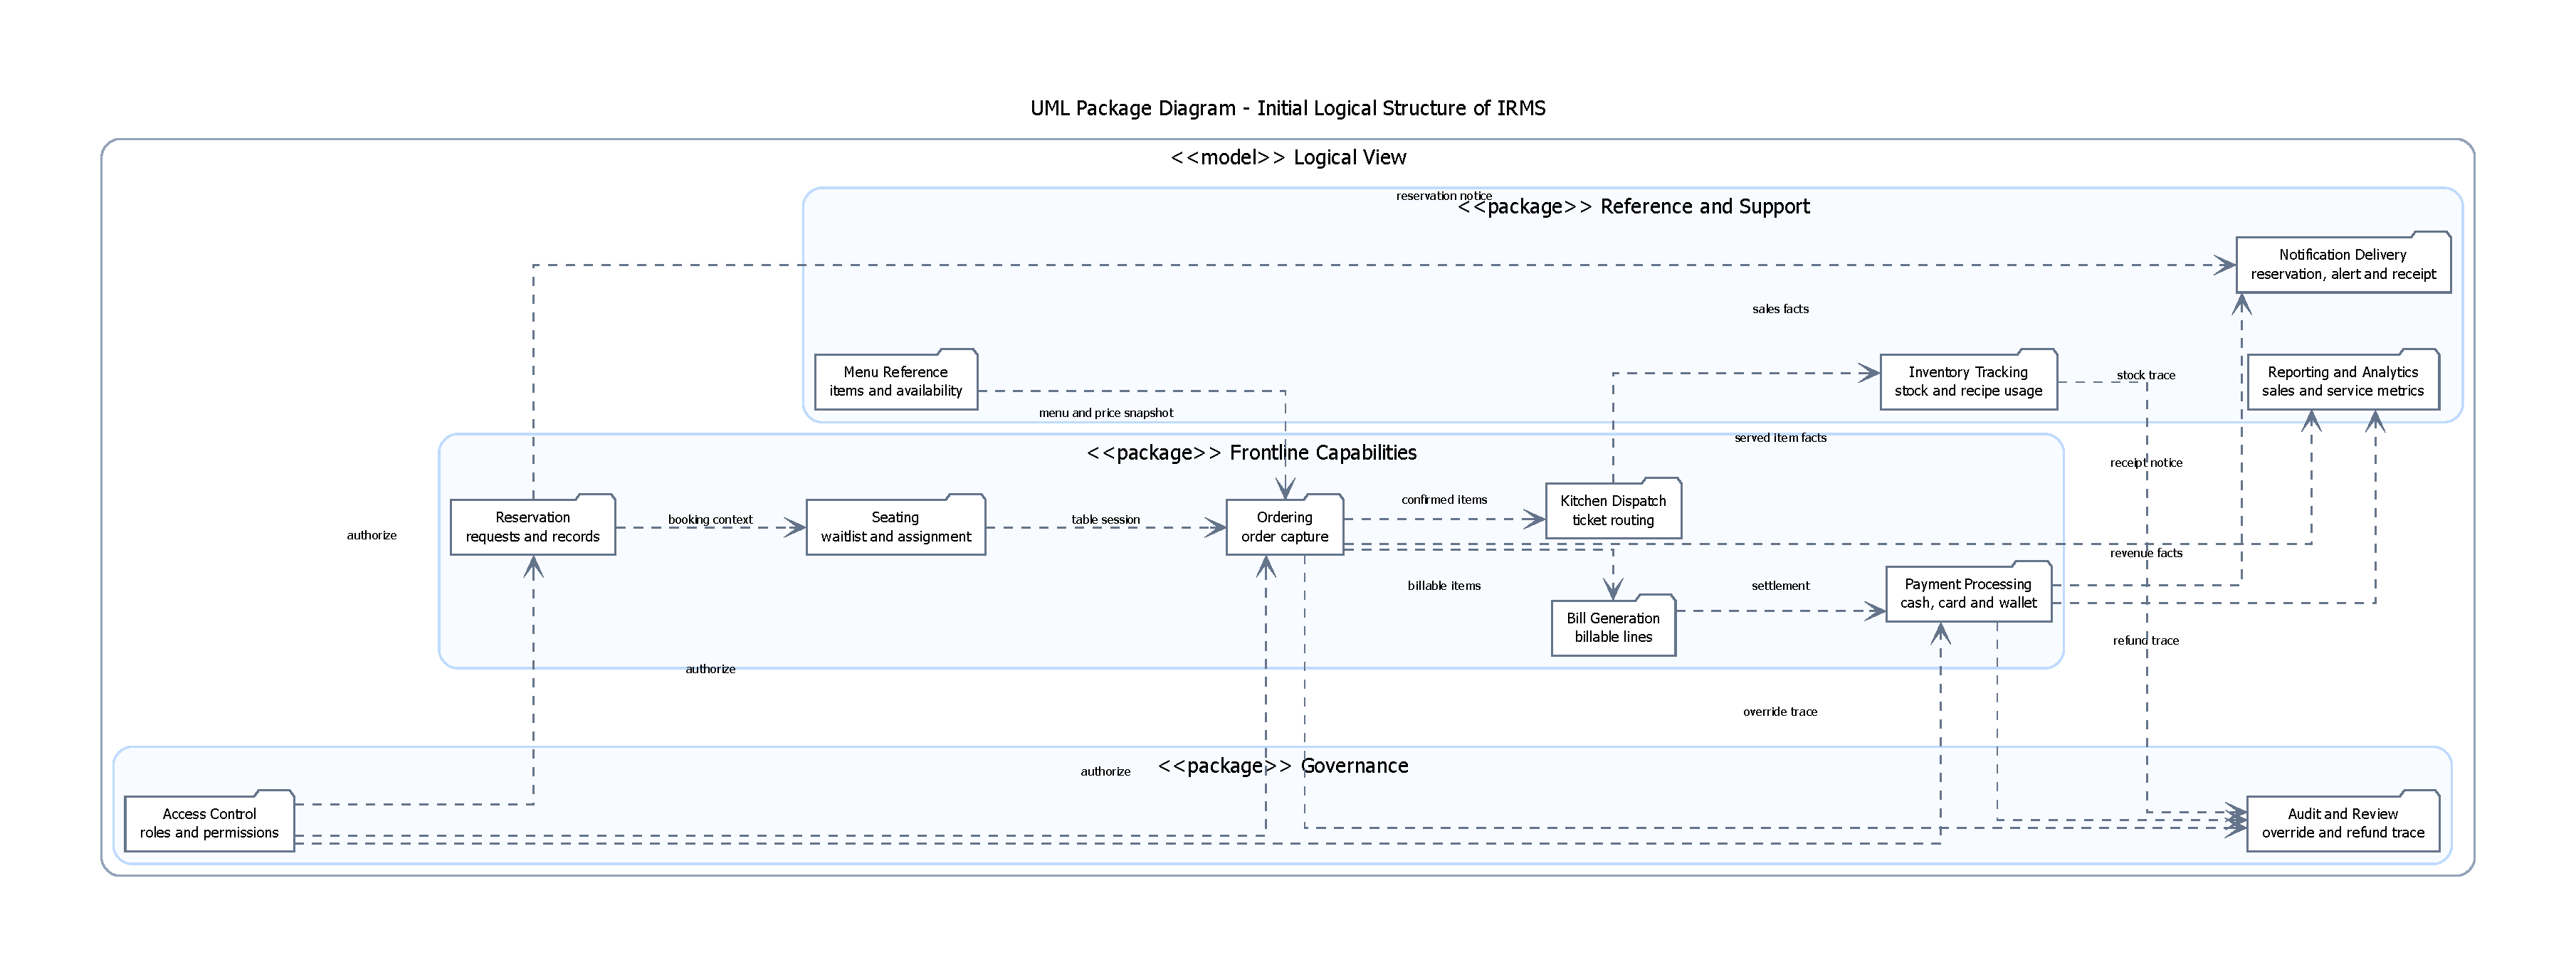
\includegraphics[width=\textwidth,height=0.78\textheight,keepaspectratio]{04_initial_logical_components_cua_irms.pdf}
}{
  \IfFileExists{04_initial_logical_components_cua_irms.png}{
    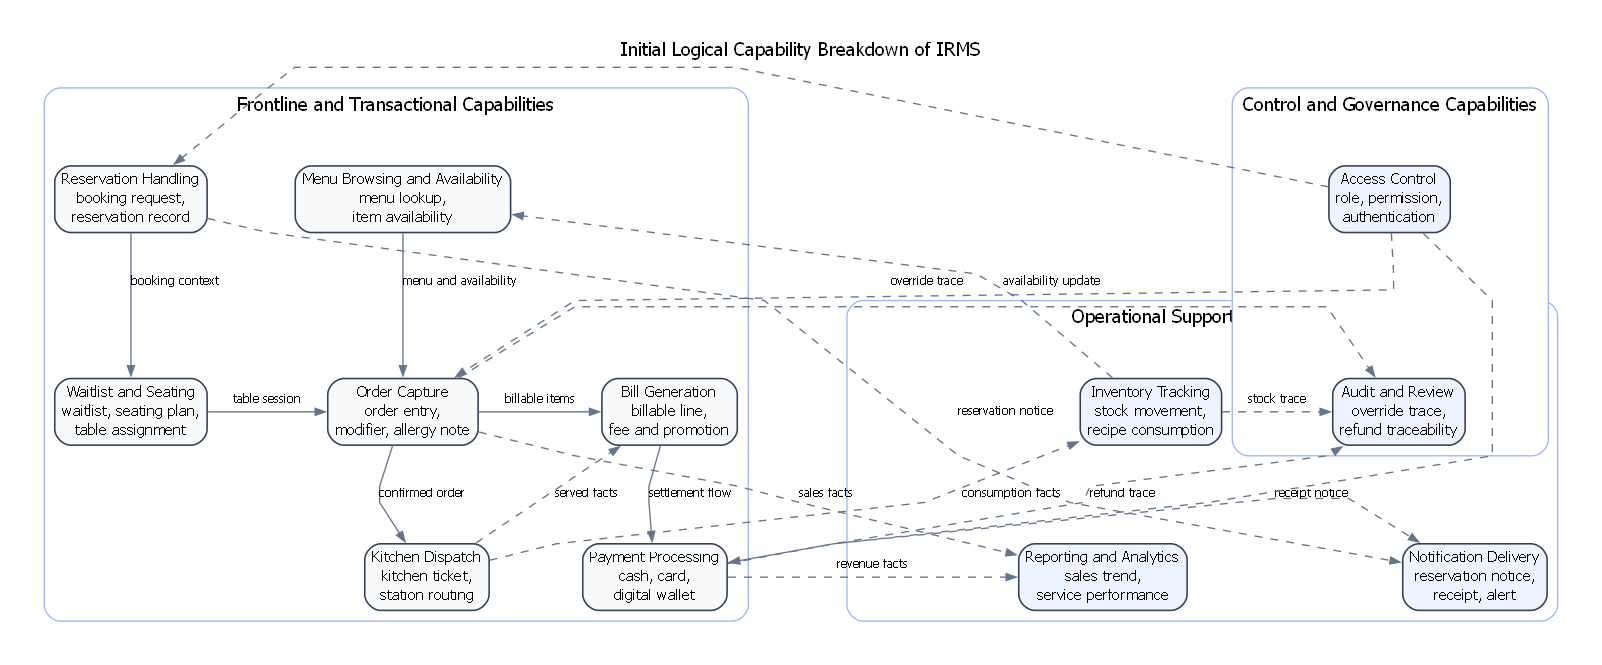
\includegraphics[width=\textwidth,height=0.78\textheight,keepaspectratio]{04_initial_logical_components_cua_irms.png}
  }{
    \fbox{\parbox{0.82\linewidth}{Thiếu file \texttt{04\_initial\_logical\_components\_cua\_irms.(pdf/png)}.}}
  }
}
\caption{Sơ đồ phân rã năng lực logic}
\label{fig:irms-initial-components}
\end{figure}

Hình~\ref{fig:irms-initial-components} thể hiện bước phân rã ban đầu các năng lực nghiệp vụ trong hệ thống IRMS.

Trong sơ đồ này, các năng lực được xác định theo hướng chức năng bề mặt như quản lý bàn, tiếp nhận đơn gọi món, điều phối bếp, thanh toán, quản lý tồn kho, báo cáo, kiểm soát truy cập và giám sát hệ thống. 

Mục tiêu là nhận diện đầy đủ phạm vi năng lực của hệ thống IRMS. Các năng lực được mô tả theo cách gần với quy trình vận hành thực tế để dễ kiểm tra và tránh bỏ sót chức năng quan trọng.

Sơ đồ này được xem là bước khởi tạo trong quá trình phân tích logic, đóng vai trò nền tảng để tiếp tục tái cấu trúc và gom nhóm các năng lực thành các miền nghiệp vụ ổn định hơn ở bước tiếp theo.
\subsubsection{Sơ đồ phân rã năng lực logic hoàn chỉnh}

\begin{figure}[H]
\centering
\IfFileExists{05_refined_logical_components_cua_irms.pdf}{
  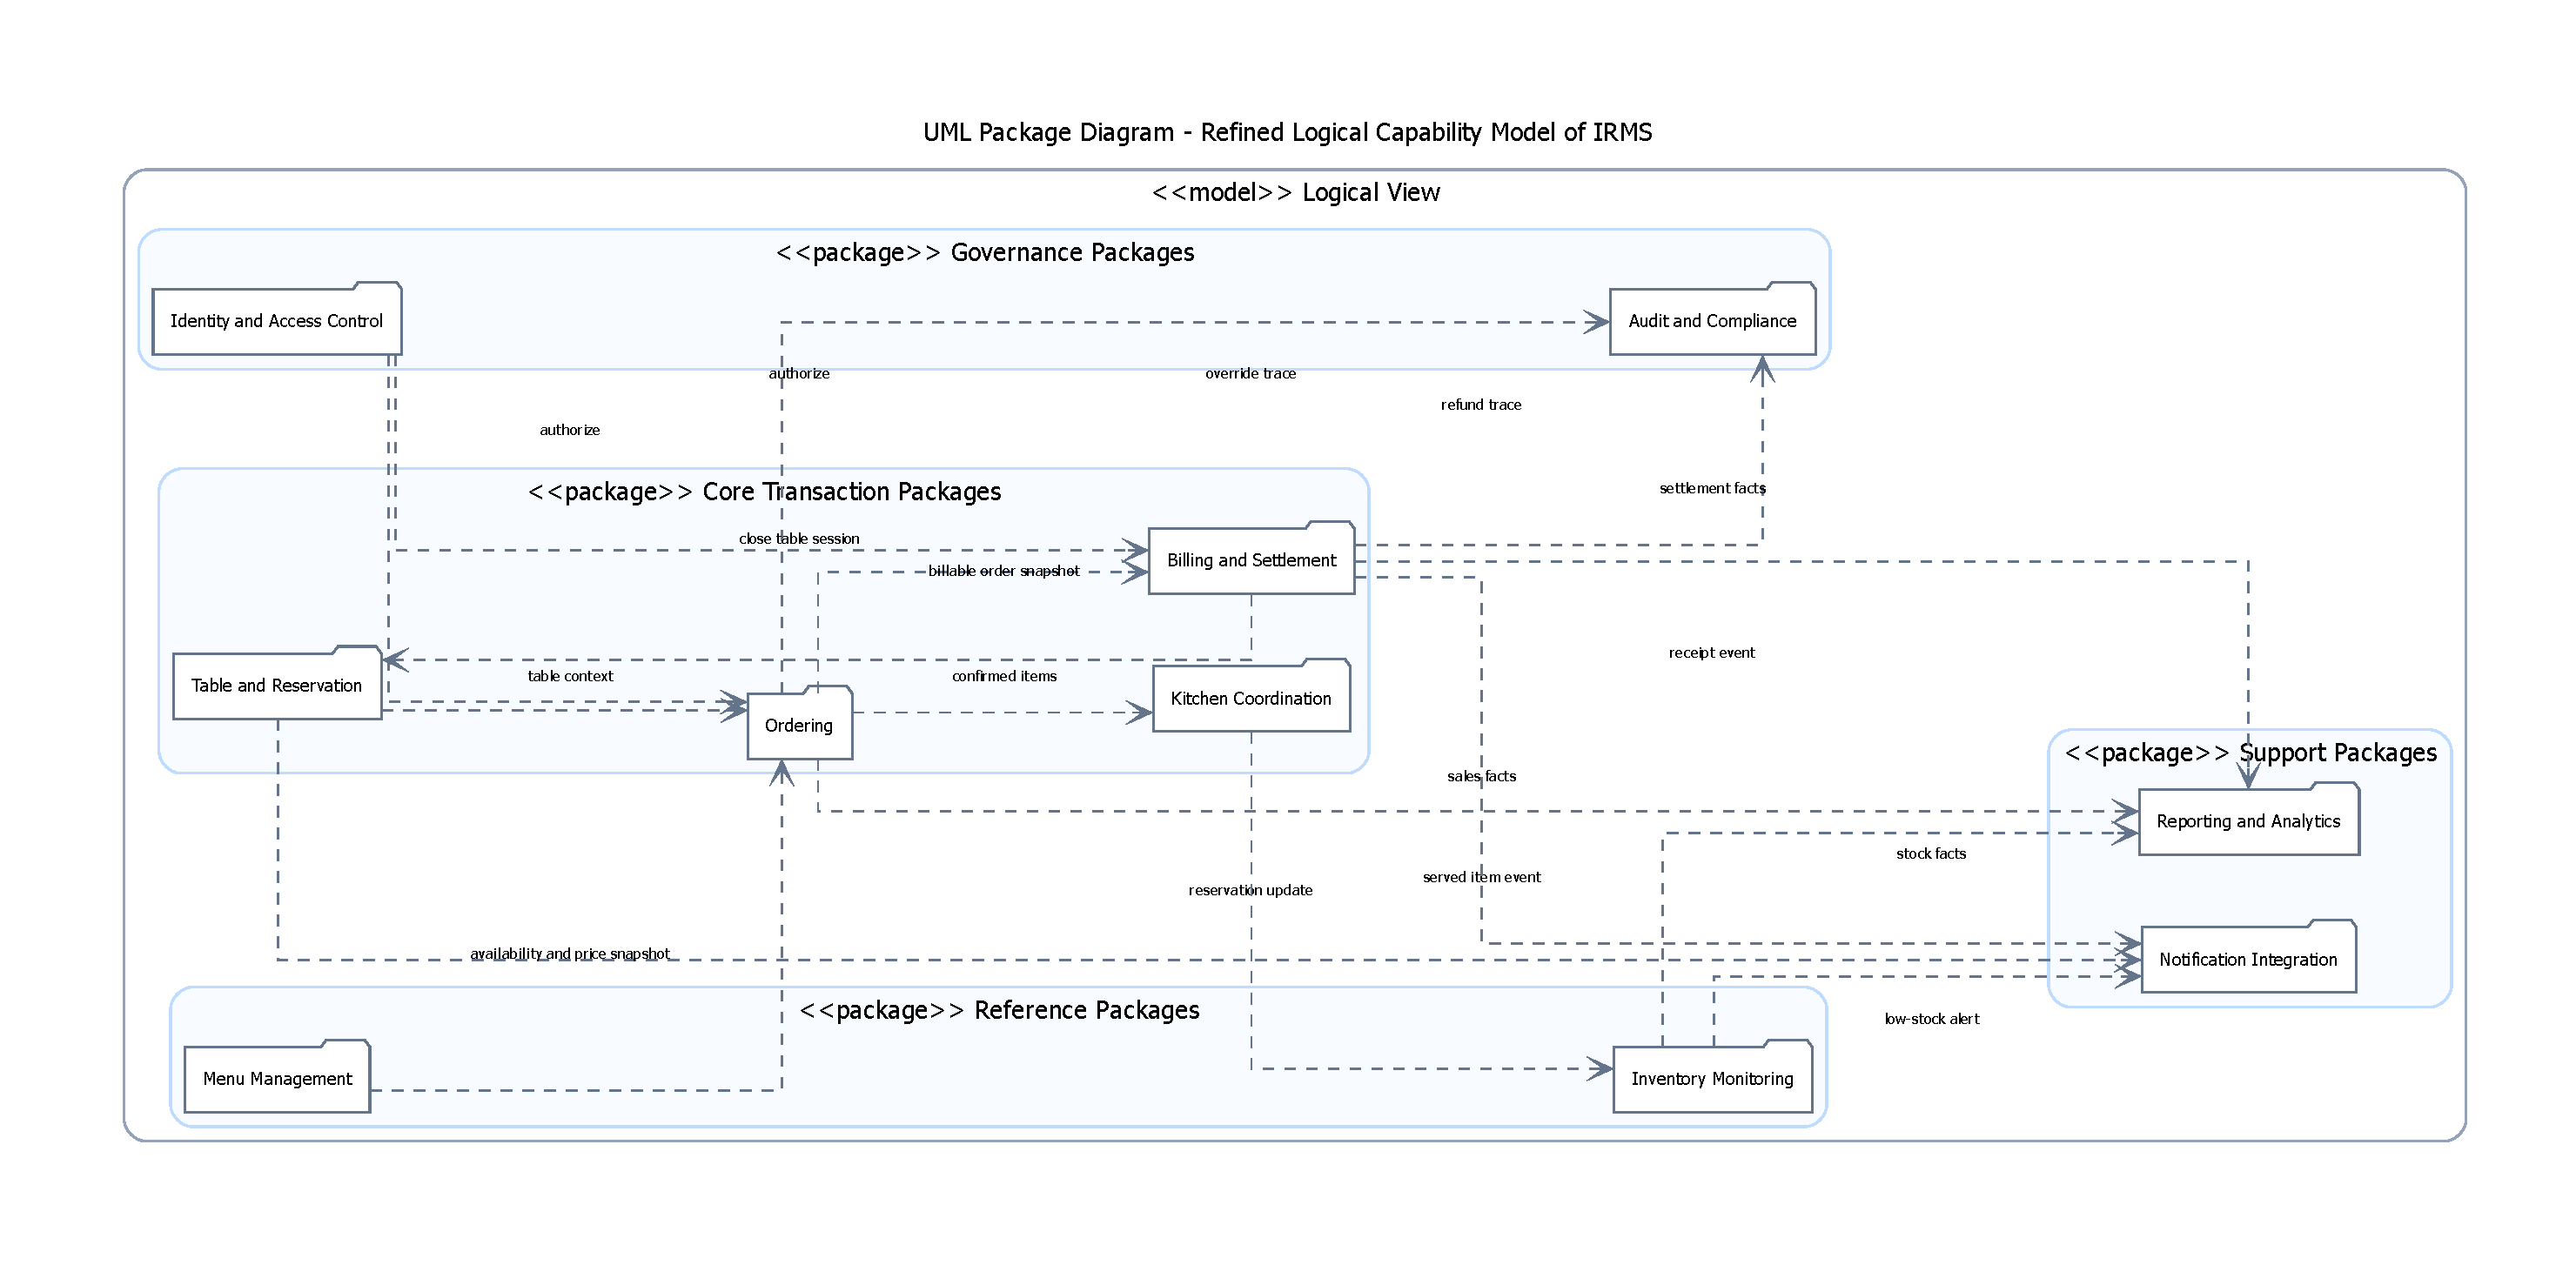
\includegraphics[width=\textwidth,height=0.78\textheight,keepaspectratio]{05_refined_logical_components_cua_irms.pdf}
}{
  \IfFileExists{05_refined_logical_components_cua_irms.png}{
    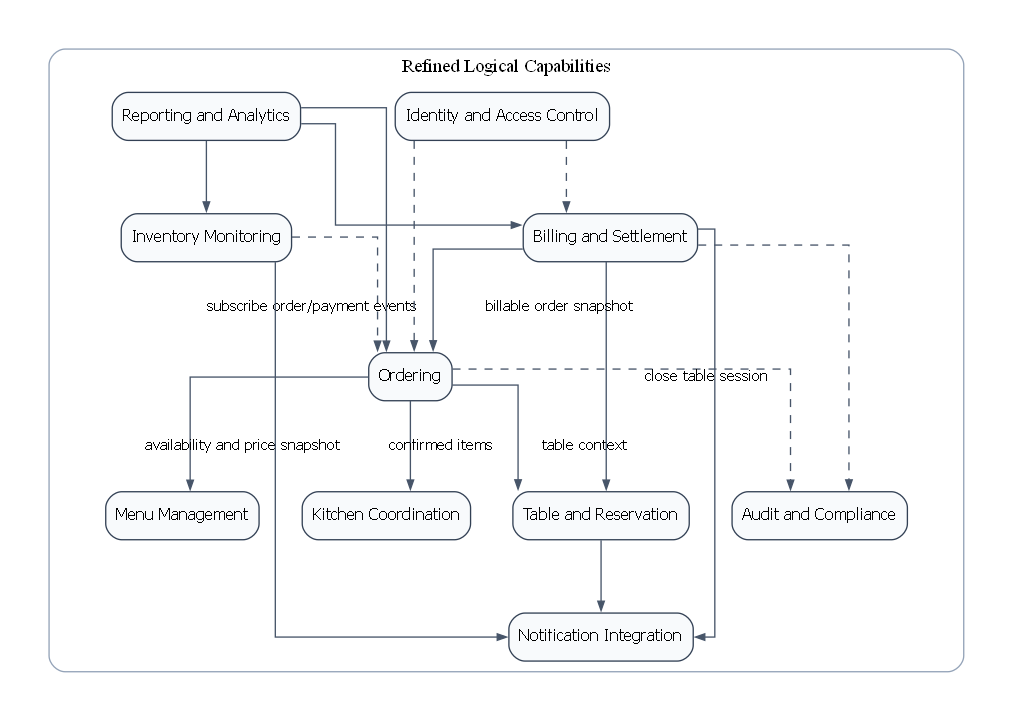
\includegraphics[width=\textwidth,height=0.78\textheight,keepaspectratio]{05_refined_logical_components_cua_irms.png}
  }{
    \fbox{\parbox{0.82\linewidth}{Thiếu file \texttt{05\_refined\_logical\_components\_cua\_irms.(pdf/png)}.}}
  }
}
\caption{Sơ đồ phân rã năng lực logic của IRMS}
\label{fig:irms-refined-components}
\end{figure}
Trong cấu trúc này, các chức năng được tổ chức theo các miền nghiệp vụ có tính kết dính cao và phản ánh đầy đủ quy trình vận hành của nhà hàng, bao gồm:
\begin{itemize}
    \item Table \& Reservation
    \item Menu Management
    \item Ordering
    \item Kitchen Coordination
    \item Billing \& Settlement
    \item Inventory Monitoring
    \item Reporting \& Analytics
    \item Identity \& Access Control
    \item Audit \& Compliance
    \item Notification Integration
\end{itemize}

Việc tái cấu trúc này giúp chuyển từ cách nhìn theo chức năng thao tác người dùng sang cách nhìn theo miền trách nhiệm nghiệp vụ. Thay vì xem hệ thống như tập hợp các chức năng rời rạc, mỗi năng lực được định nghĩa như một miền logic độc lập, có ranh giới rõ ràng và chịu trách nhiệm cho một phần xác định trong vòng đời vận hành của nhà hàng.

Từ góc độ kiến trúc, đây là bước chuyển từ functional decomposition sang domain-oriented decomposition. Các năng lực lúc này không chỉ mang ý nghĩa chức năng, mà trở thành các đơn vị nghiệp vụ có tính độc lập tương đối, có thể được ánh xạ trực tiếp hoặc gián tiếp sang các service trong kiến trúc service-based.

Bên cạnh đó, cấu trúc này cũng tạo nền tảng cho mô hình event-driven processing trong các góc nhìn kiến trúc tiếp theo. Các miền năng lực có thể trao đổi thông tin thông qua sự kiện nghiệp vụ thay vì phụ thuộc trực tiếp lẫn nhau, từ đó giảm coupling giữa các thành phần và tăng khả năng mở rộng của hệ thống trong dài hạn.
\subsubsection{Sơ đồ chuỗi phục vụ}

\begin{figure}[H]
\centering
\IfFileExists{34_logical_view_core_service_chain.pdf}{
  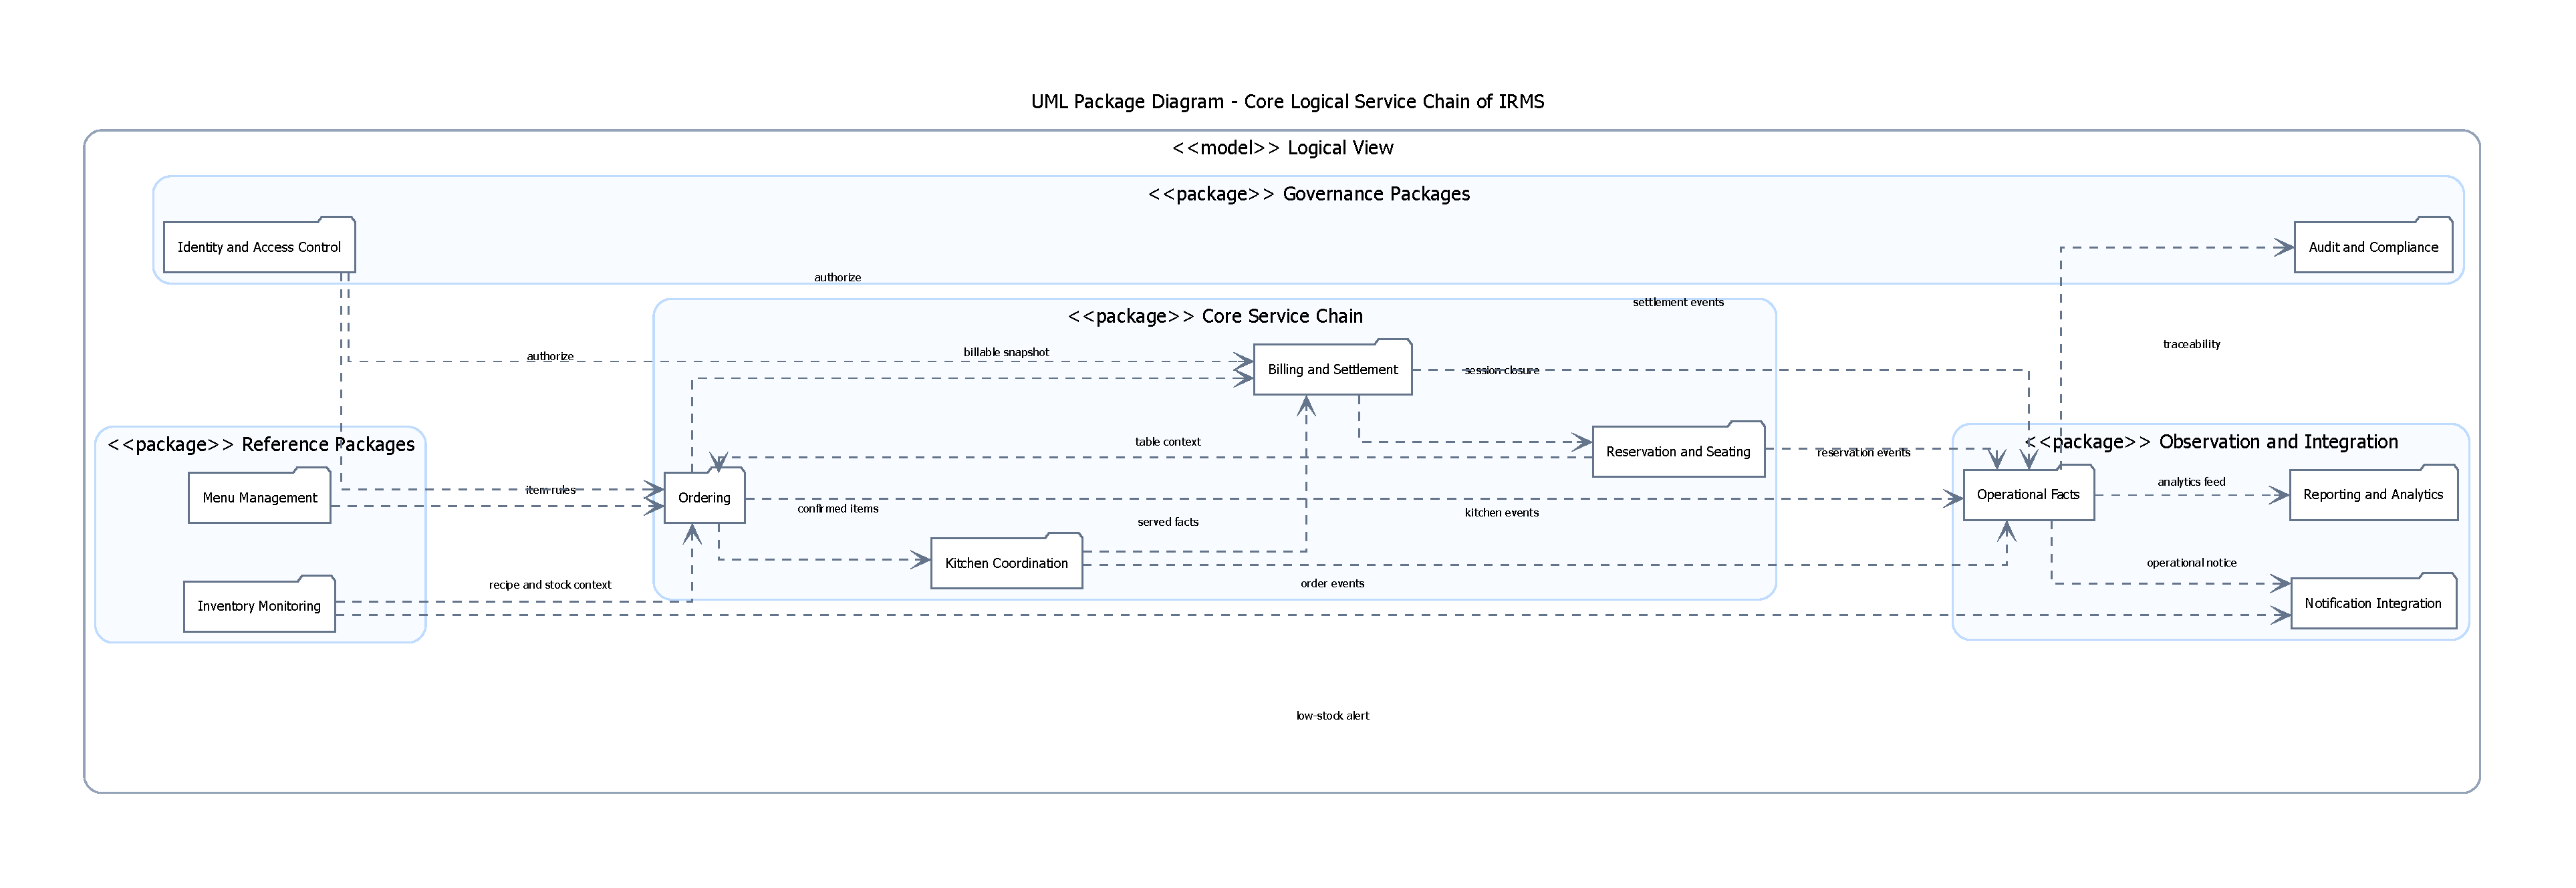
\includegraphics[width=\textwidth,height=0.84\textheight,keepaspectratio]{34_logical_view_core_service_chain.pdf}
}{
  \IfFileExists{34_logical_view_core_service_chain.png}{
    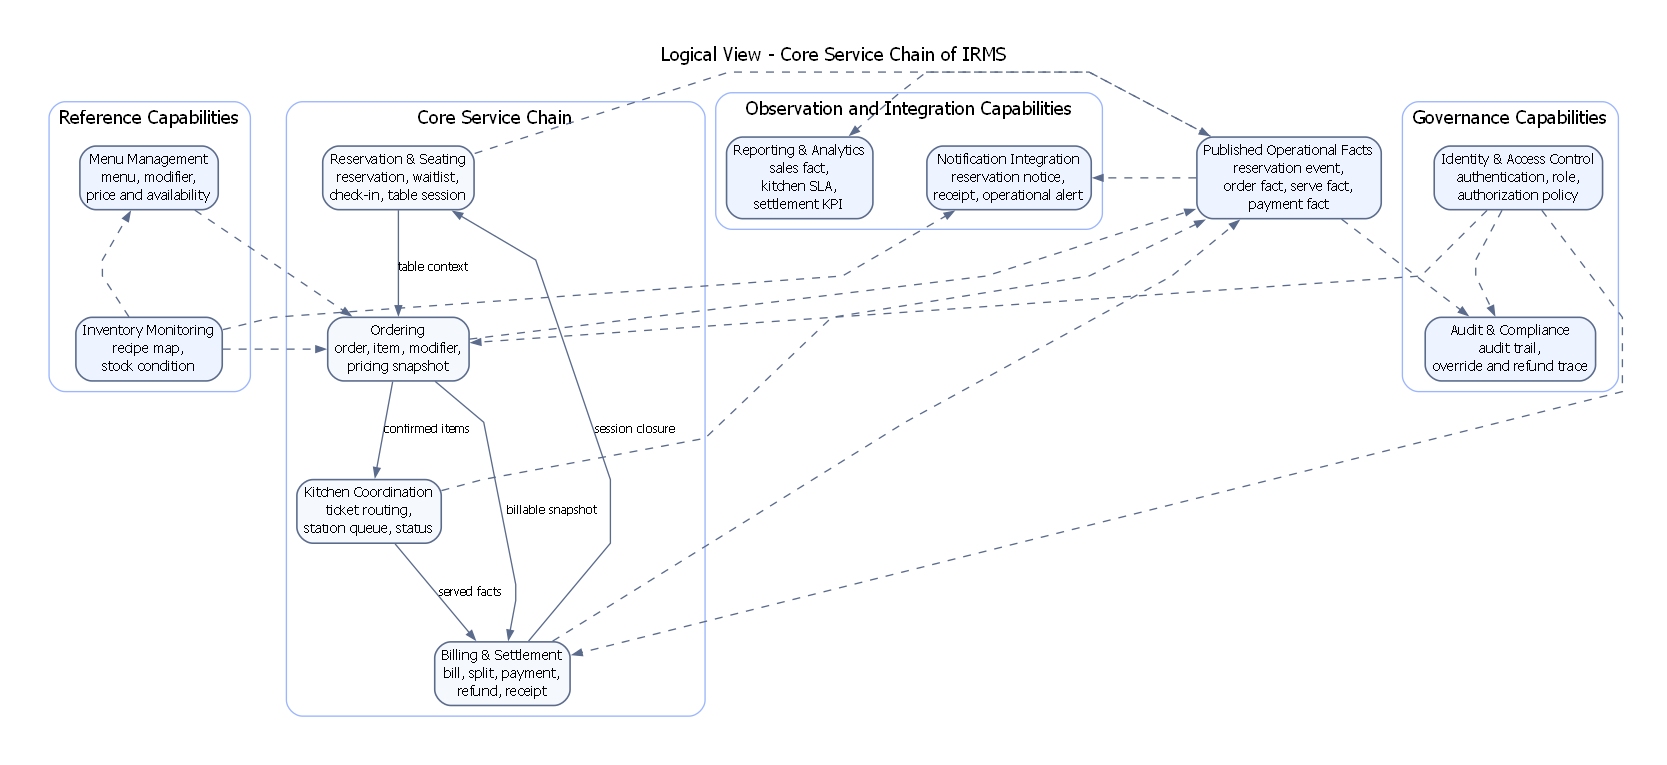
\includegraphics[width=\textwidth,height=0.84\textheight,keepaspectratio]{34_logical_view_core_service_chain.png}
  }{
    \fbox{\parbox{0.82\linewidth}{Thiếu file \texttt{34\_logical\_view\_core\_service\_chain.(pdf/png)}.}}
  }
}
\caption{Sơ đồ năng lực cho chuỗi phục vụ lõi của IRMS}
\label{fig:irms-logical-core-chain}
\end{figure}
Hình~\ref{fig:irms-logical-core-chain} mô tả cách các năng lực logic lõi tương tác với nhau trong chuỗi phục vụ chính của hệ thống.

Chuỗi này bao gồm bốn miền năng lực chính:

\begin{itemize}
    \item Reservation \& Seating: thiết lập và duy trì ngữ cảnh phục vụ
    \item Ordering: ghi nhận và quản lý đơn gọi món
    \item Kitchen Coordination: điều phối quá trình chế biến món ăn
    \item Billing \& Settlement: xử lý thanh toán và kết thúc phiên phục vụ
\end{itemize}

Sơ đồ thể hiện rằng hệ thống không vận hành như tập hợp các chức năng độc lập, mà được tổ chức theo một chuỗi năng lực có thứ tự rõ ràng, phản ánh trực tiếp vòng đời phục vụ của nhà hàng. Mỗi năng lực tương ứng với một giai đoạn trong quy trình nghiệp vụ tổng thể và chỉ chịu trách nhiệm trong phạm vi của giai đoạn đó.

Trong chuỗi này, các miền nghiệp vụ chỉ trao đổi lượng thông tin tối thiểu cần thiết để đảm bảo tính nhất quán của luồng xử lý. Reservation \& Seating cung cấp ngữ cảnh phiên bàn hợp lệ; Ordering tạo và xác nhận thông tin đơn gọi món; Kitchen Coordination tiếp nhận và xử lý trạng thái chế biến; trong khi Billing \& Settlement sử dụng dữ liệu đã được chốt để thực hiện quyết toán và kết thúc phiên phục vụ.

Cách tổ chức này giúp đảm bảo luồng nghiệp vụ chính có tính tuyến tính và dễ kiểm soát, đồng thời giảm thiểu sự phụ thuộc trực tiếp giữa các miền nghiệp vụ. Về mặt kiến trúc, đây là cơ sở để hiện thực hóa các tương tác giữa các năng lực thông qua cơ chế gọi dịch vụ đồng bộ trong luồng chính và cơ chế sự kiện nghiệp vụ (domain events) cho các tương tác mở rộng trong các góc nhìn triển khai phía sau.

\subsection{Góc nhìn phân rã}\label{sec:module-view}
Ở góc nhìn phân rã, hệ thống được chia thành hai lớp lớn:
\textbf{các ứng dụng phía người dùng} và \textbf{các service nghiệp vụ }.

\subsubsection{Các ứng dụng phía người dùng}
\begin{itemize}
  \item \textbf{Host/Reservation UI}: phục vụ đặt bàn, danh sách chờ, sơ đồ bàn và check-in.
  \item \textbf{Server POS UI}: phục vụ gọi món tại bàn, thay đổi món, theo dõi phiếu bếp và thực hiện tính tiền.
  \item \textbf{Kitchen Display UI}: hiển thị phiếu bếp theo trạm, mức ưu tiên, thời gian dự kiến hoàn thành và tiến độ chế biến.
  \item \textbf{Cashier UI}: tạo hóa đơn, tách hóa đơn, thanh toán, biên lai và hoàn tiền.
  \item \textbf{Manager Portal}: quản lý thực đơn, chương trình khuyến mãi, cảnh báo tồn kho, lịch làm việc và báo cáo.
\end{itemize}

\subsubsection{Các dịch vụ nghiệp vụ }
\begin{itemize}
  \item \textbf{Reservation \& Seating Service}: quản lý đặt bàn, danh sách chờ, bàn ăn và phiên phục vụ tại bàn.
  \item \textbf{Ordering Service}: quản lý thực đơn, tùy chọn món, đơn gọi món, dòng món và trạng thái của đơn từ đầu đến cuối.
  \item \textbf{Kitchen Coordination Service}: điều phối phiếu bếp, trạm bếp và cam kết thời gian ra món.
  \item \textbf{Billing Service}: quản lý hóa đơn, tách hóa đơn, thanh toán, biên lai, hoàn tiền và áp dụng khuyến mãi.
  \item \textbf{Inventory Service}: quản lý công thức, mặt hàng tồn kho, giao dịch kho và quy tắc cảnh báo mức tồn thấp.
  \item \textbf{Reporting Service}: quản lý mô hình đọc, ảnh chụp dữ liệu báo cáo và xuất báo cáo.
  \item \textbf{IAM/Access Service}: định danh, vai trò, quyền và thực thi chính sách truy cập.
\end{itemize}


\subsubsection{Sơ đồ tổng quan}
\begin{figure}[H]
\centering
\IfFileExists{06_module_view_overall_irms.pdf}{
  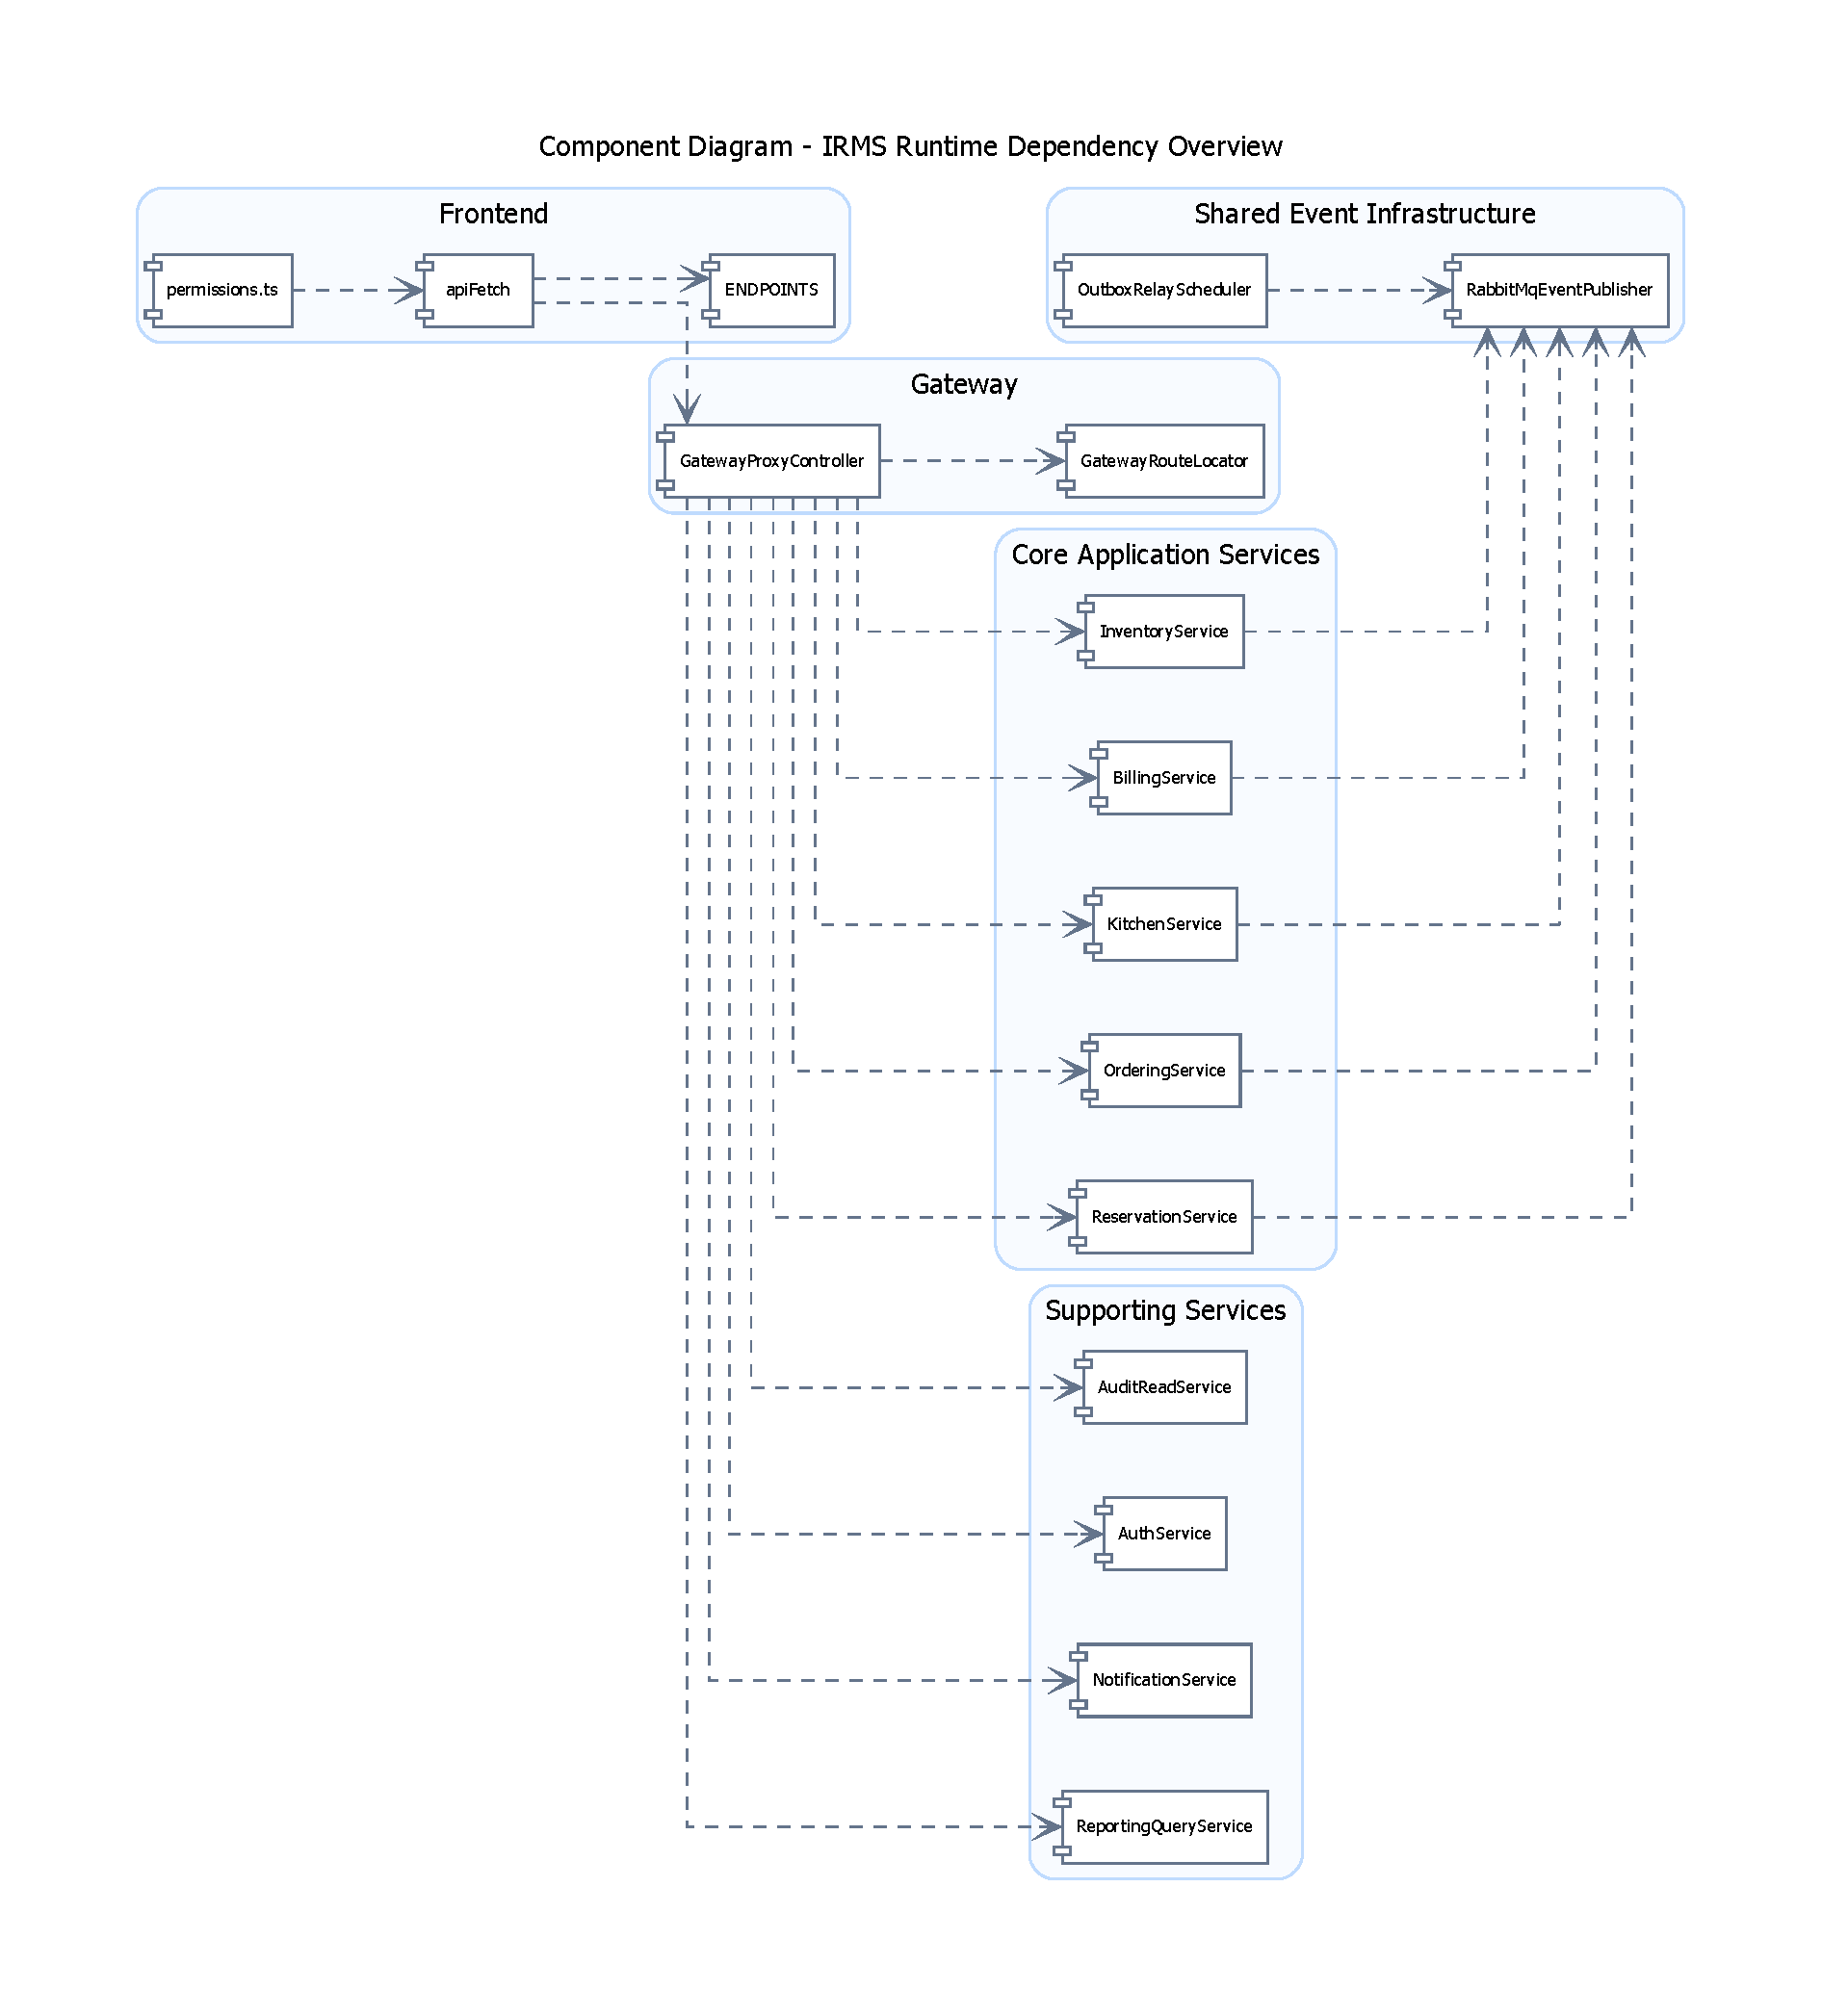
\includegraphics[width=\textwidth,height=0.82\textheight,keepaspectratio]{06_module_view_overall_irms.pdf}
}{
  \IfFileExists{06_module_view_overall_irms.png}{
    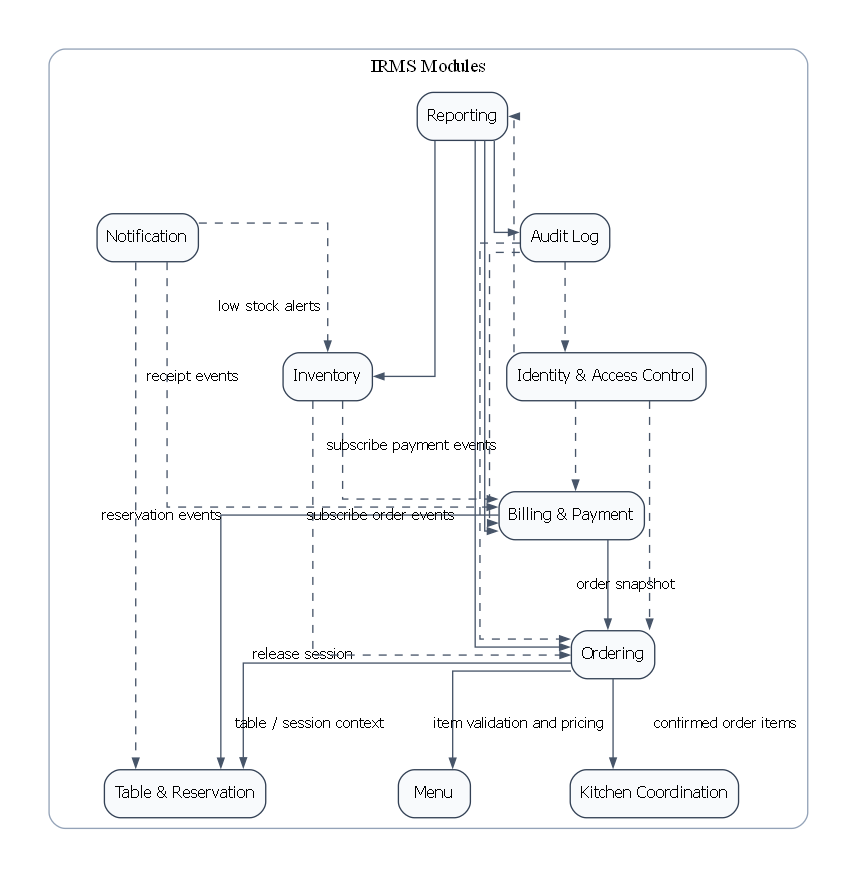
\includegraphics[width=\textwidth,height=0.82\textheight,keepaspectratio]{06_module_view_overall_irms.png}
  }{
    \fbox{\parbox{0.82\linewidth}{Thiếu file \textsf{06\_module\_view\_overall\_irms.(pdf/png)}.}}
  }
}
\caption{Module View tổng quan theo package backend của IRMS}
\label{fig:irms-module-overall}
\end{figure}

Sơ đồ thể hiện \textbf{cách các package và class trung tâm được chia theo nghĩa nghiệp vụ}. \textsf{ReservationService} đại diện cho vùng đặt bàn; \textsf{OrdersService} xử lý tạo và xác nhận đơn; \textsf{KitchenService} xử lý trạng thái phiếu bếp; \textsf{BillingService} xử lý lập hóa đơn; còn \textsf{InventoryService}, \textsf{ReportingQueryService}, \textsf{NotificationService}, \textsf{AuthService} và \textsf{AuditService} giữ các vùng hỗ trợ và kiểm soát.

Một điểm quan trọng khác của sơ đồ là \textbf{các phụ thuộc giữa thành phần}. \textsf{apiFetch} gọi các endpoint đã khai báo trong \textsf{ENDPOINTS}, sau đó \textsf{GatewayProxyController} định tuyến đến service phù hợp. Các service nghiệp vụ cùng phát sự kiện qua \textsf{RabbitMqEventPublisher}, còn \textsf{RabbitMqOutboxRelay} xử lý phần chuyển tiếp nền. 

\paragraph{Mô tả}
\begin{itemize}
  \item \textbf{Các thành phần frontend và gateway}: \textsf{apiFetch}, \textsf{ENDPOINTS}, \textsf{permissions.ts}, \textsf{GatewayProxyController} và \textsf{GatewayRouteLocator}.
  \item \textbf{Các service ứng dụng}: \textsf{ReservationService}, \textsf{OrdersService}, \textsf{KitchenService}, \textsf{BillingService}, \textsf{InventoryService}, \textsf{ReportingQueryService}, \textsf{NotificationService}, \textsf{AuthService} và \textsf{AuditService}.
  \item \textbf{Các thành phần sự kiện dùng chung}: \textsf{RabbitMqEventPublisher} và \textsf{RabbitMqOutboxRelay}.
\end{itemize}



\begin{figure}[H]
\centering
\IfFileExists{07_module_view_core_fulfillment_path.pdf}{
  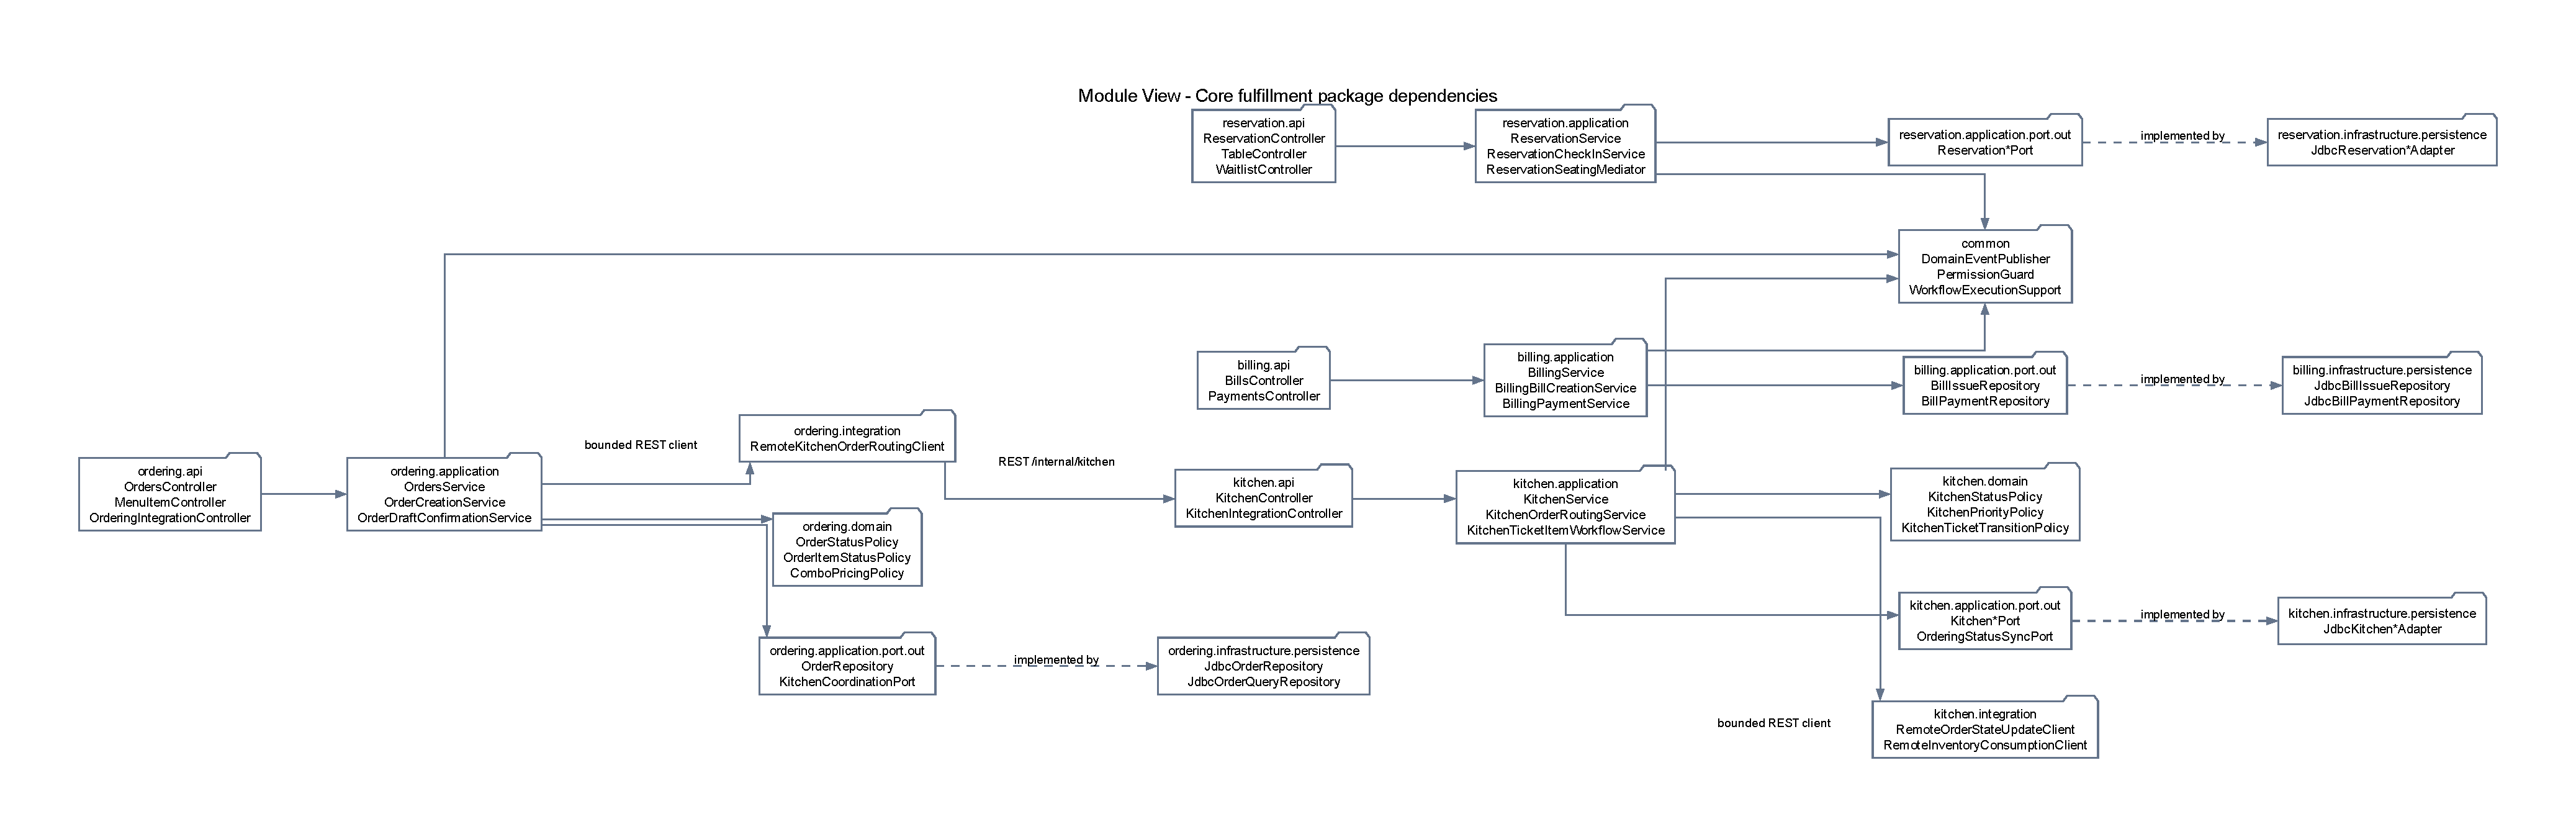
\includegraphics[width=0.97\linewidth,height=0.84\textheight,keepaspectratio]{07_module_view_core_fulfillment_path.pdf}
}{
  \IfFileExists{07_module_view_core_fulfillment_path.png}{
    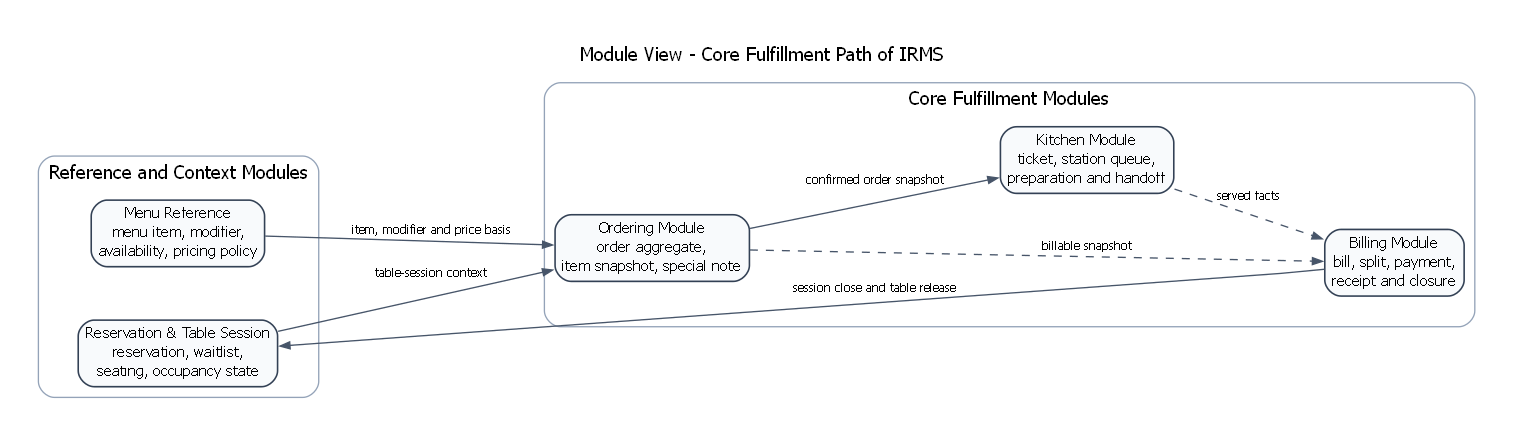
\includegraphics[width=0.97\linewidth,height=0.84\textheight,keepaspectratio]{07_module_view_core_fulfillment_path.png}
  }{
    \fbox{\parbox{0.82\linewidth}{Thiếu file \textsf{07\_module\_view\_core\_fulfillment\_path.(pdf/png)}.}}
  }
}
\caption{Module View chi tiết cho tuyến xử lý nghiệp vụ lõi}
\label{fig:irms-module-core}
\end{figure}



Trong cấu trúc này, \textsf{OrdersService} được đặt ở trung tâm để phản ánh vai trò cốt lõi của nghiệp vụ gọi món, nơi hệ thống phải kiểm tra trạng thái bàn, tính hợp lệ của món và tùy chọn, đồng thời chuyển thông tin sang bếp thông qua \textsf{RemoteKitchenOrderRoutingClient}. Service này tập trung vào xử lý dữ liệu gọi món và điều phối nghiệp vụ trực tiếp, tránh trở thành nơi chứa toàn bộ logic như khuyến mãi, tồn kho, thông báo hay phân tích.

Mối quan hệ giữa \textsf{OrdersService}, \textsf{KitchenOrderRoutingService} và \textsf{BillingBillCreationService} cũng thể hiện luồng nghiệp vụ rõ ràng: từ xác nhận đơn gọi món, sang điều phối chế biến tại bếp, rồi đến lập hóa đơn và thanh toán. Các service phía sau sử dụng dữ liệu đáng tin cậy từ đơn gọi món nhưng không can thiệp ngược vào cấu trúc nghiệp vụ gốc.
\paragraph{Mô tả}
\begin{itemize}
  \item \textbf{\textsf{ReservationCheckInService} và \textsf{ReservationTableAssignmentService}}: cung cấp ngữ cảnh bàn đang phục vụ.
  \item \textbf{\textsf{OrdersService}}: giữ vai trò trục trung tâm của tuyến nghiệp vụ nóng.
  \item \textbf{\textsf{KitchenOrderRoutingService} và \textsf{BillingBillCreationService}}: là hai hướng lan truyền quan trọng sau khi đơn được xác nhận.
\end{itemize}



\begin{figure}[H]
\centering
\IfFileExists{08_module_view_support_and_cross_cutting_modules.pdf}{
  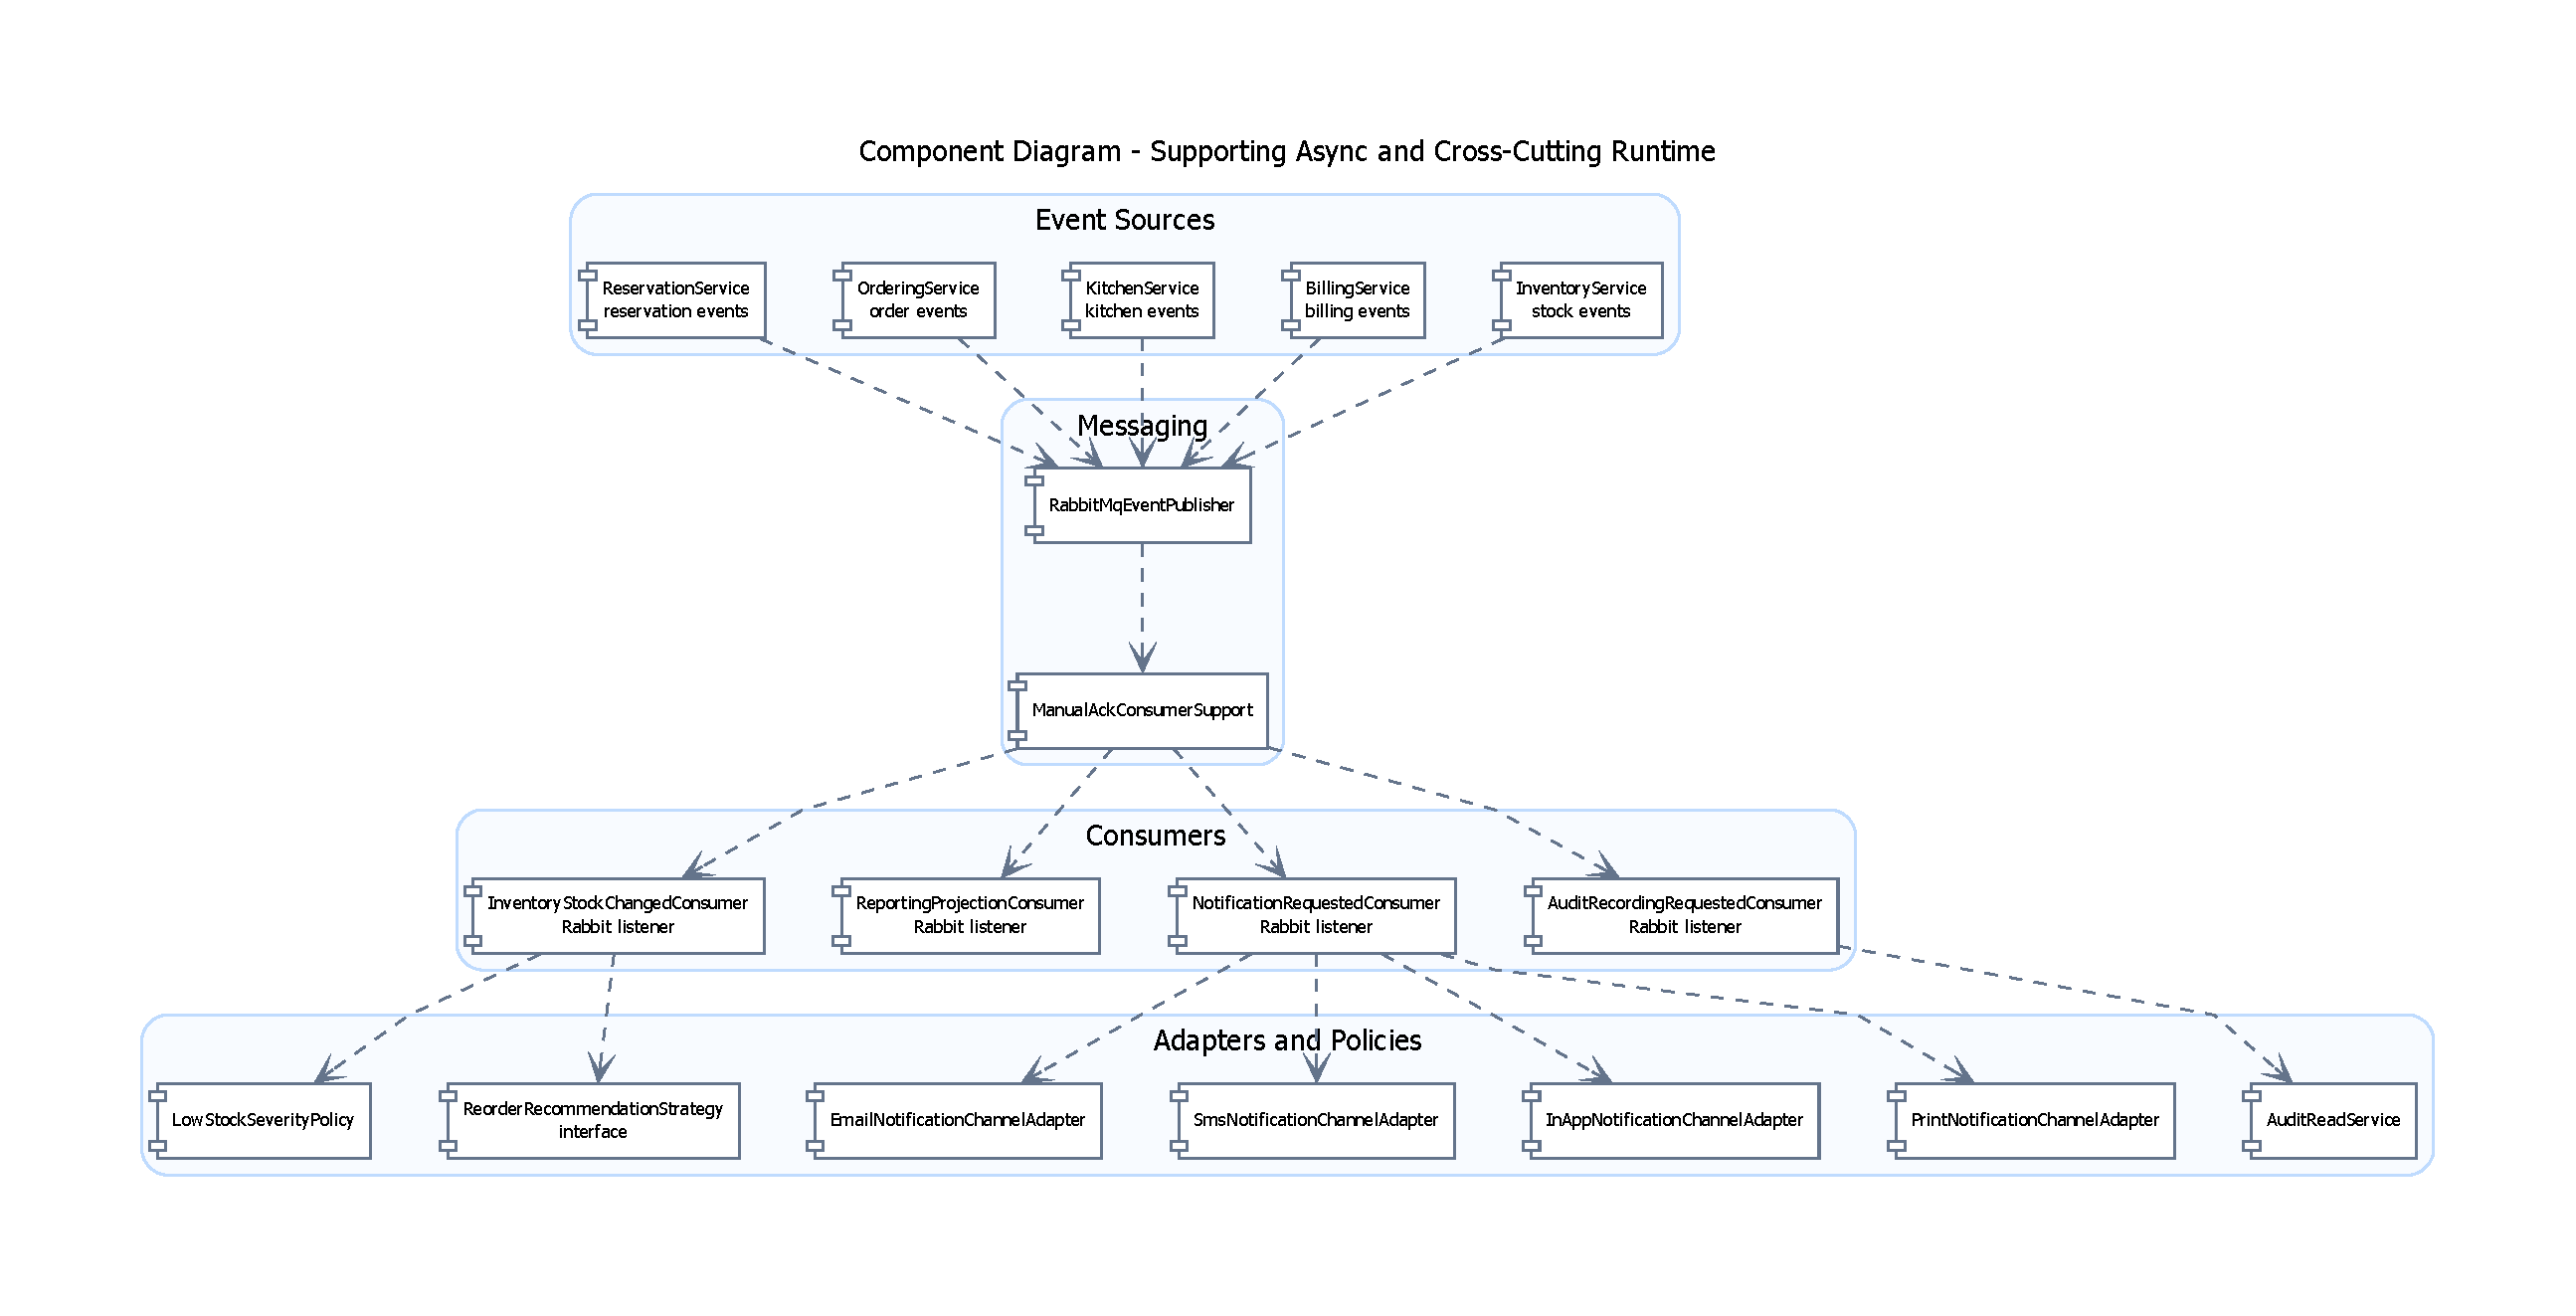
\includegraphics[width=0.97\linewidth,height=0.84\textheight,keepaspectratio]{08_module_view_support_and_cross_cutting_modules.pdf}
}{
  \IfFileExists{08_module_view_support_and_cross_cutting_modules.png}{
    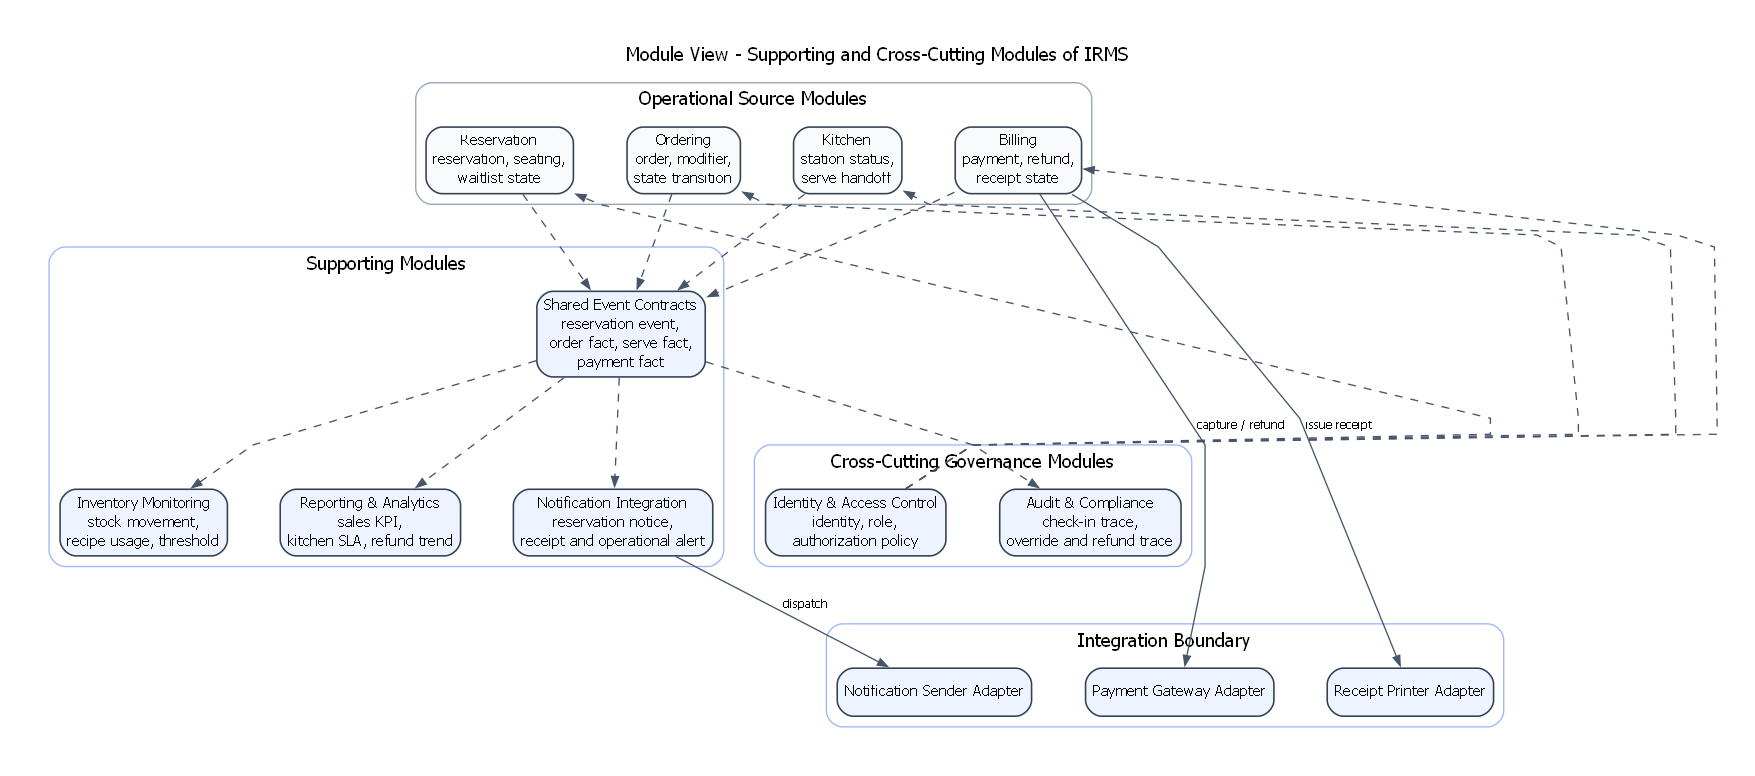
\includegraphics[width=0.97\linewidth,height=0.84\textheight,keepaspectratio]{08_module_view_support_and_cross_cutting_modules.png}
  }{
    \fbox{\parbox{0.82\linewidth}{Thiếu file \textsf{08\_module\_view\_support\_and\_cross\_cutting\_modules.(pdf/png)}.}}
  }
}
\caption{Module View cho các package hỗ trợ và xuyên suốt}
\label{fig:irms-module-support}
\end{figure}

Hình trên mô tả các package hỗ trợ và các thành phần xử lý nền của hệ thống. Đây là những thành phần không nằm trực tiếp trong các giao dịch chính như gọi món hay thanh toán, nhưng vẫn đóng vai trò quan trọng đối với vận hành và quản lý hệ thống. Góc nhìn này tập trung vào các module liên quan đến messaging, event processing và runtime support thay vì các lớp nghiệp vụ lõi.

Trong kiến trúc IRMS, các consumer như \textsf{InventoryStockChangedConsumer}, \textsf{ReportingProjectionConsumer}, \textsf{NotificationRequestedConsumer} và \textsf{AuditRecordingRequestedConsumer} đảm nhận các chức năng khác nhau. \textsf{InventoryStockChangedConsumer} cập nhật biến động tồn kho dựa trên dữ liệu vận hành; \textsf{ReportingProjectionConsumer} xây dựng dữ liệu phục vụ báo cáo; \textsf{NotificationRequestedConsumer} xử lý việc gửi thông báo; còn \textsf{AuditRecordingRequestedConsumer} ghi nhận dữ liệu kiểm toán và theo dõi thao tác trong hệ thống.

Các thành phần này nhận dữ liệu sự kiện từ các service nghiệp vụ như \textsf{ReservationService}, \textsf{OrdersService}, \textsf{KitchenService}, \textsf{BillingService} và \textsf{InventoryService} thông qua \textsf{RabbitMqEventPublisher}. Nhờ đó, các chức năng hỗ trợ có thể được xử lý bất đồng bộ mà không ảnh hưởng trực tiếp đến các giao dịch chính.

Việc tách riêng các service hỗ trợ giúp hệ thống dễ mở rộng và thuận tiện hơn cho quản trị vận hành. Các chức năng như báo cáo, cảnh báo tồn kho, phân quyền hay kiểm toán có thể hoạt động độc lập với tuyến xử lý chính của hệ thống.

Tuy nhiên, cách tổ chức này cũng dẫn đến độ trễ nhất định trong các chức năng hỗ trợ. Ví dụ, dữ liệu báo cáo hoặc cảnh báo tồn kho có thể cập nhật chậm hơn vài giây so với giao dịch thực tế. Đánh đổi này được chấp nhận vì các thao tác cần phản hồi ngay trong nhà hàng vẫn là đặt bàn, gọi món, chế biến và thanh toán.
\paragraph{Các thành phần chính trong hình.}
\begin{itemize}
  \item \textbf{\textsf{ReservationService}, \textsf{OrdersService}, \textsf{KitchenService}, \textsf{BillingService} và \textsf{InventoryService}}: là các thành phần nguồn phát sinh dữ kiện vận hành để nhóm hỗ trợ tiêu thụ.
  \item \textbf{\textsf{RabbitMqEventPublisher} và \textsf{ManualAckConsumerSupport}}: là lớp trung gian chuẩn hóa và xử lý sự kiện trước khi sang nhóm hỗ trợ.
  \item \textbf{\textsf{InventoryStockChangedConsumer}, \textsf{ReportingProjectionConsumer} và \textsf{NotificationRequestedConsumer}}: đại diện cho nhóm suy diễn, tổng hợp và tích hợp có thể chạy lệch nhịp với đường nóng.
  \item \textbf{\textsf{AuditRecordingRequestedConsumer} và \textsf{AuditService}}: đại diện cho nhóm kiểm soát xuyên suốt.
  \item \textbf{Các adapter kênh thông báo}: gồm \textsf{EmailNotificationChannelAdapter}, \textsf{SmsNotificationChannelAdapter}, \textsf{InAppNotificationChannelAdapter} và \textsf{PrintNotificationChannelAdapter}.
\end{itemize}


\subsubsection{Chi tiết Module View cho tuyến order-to-cash}
\begin{figure}[H]
\centering
\IfFileExists{35_module_view_order_to_cash_slices.pdf}{
  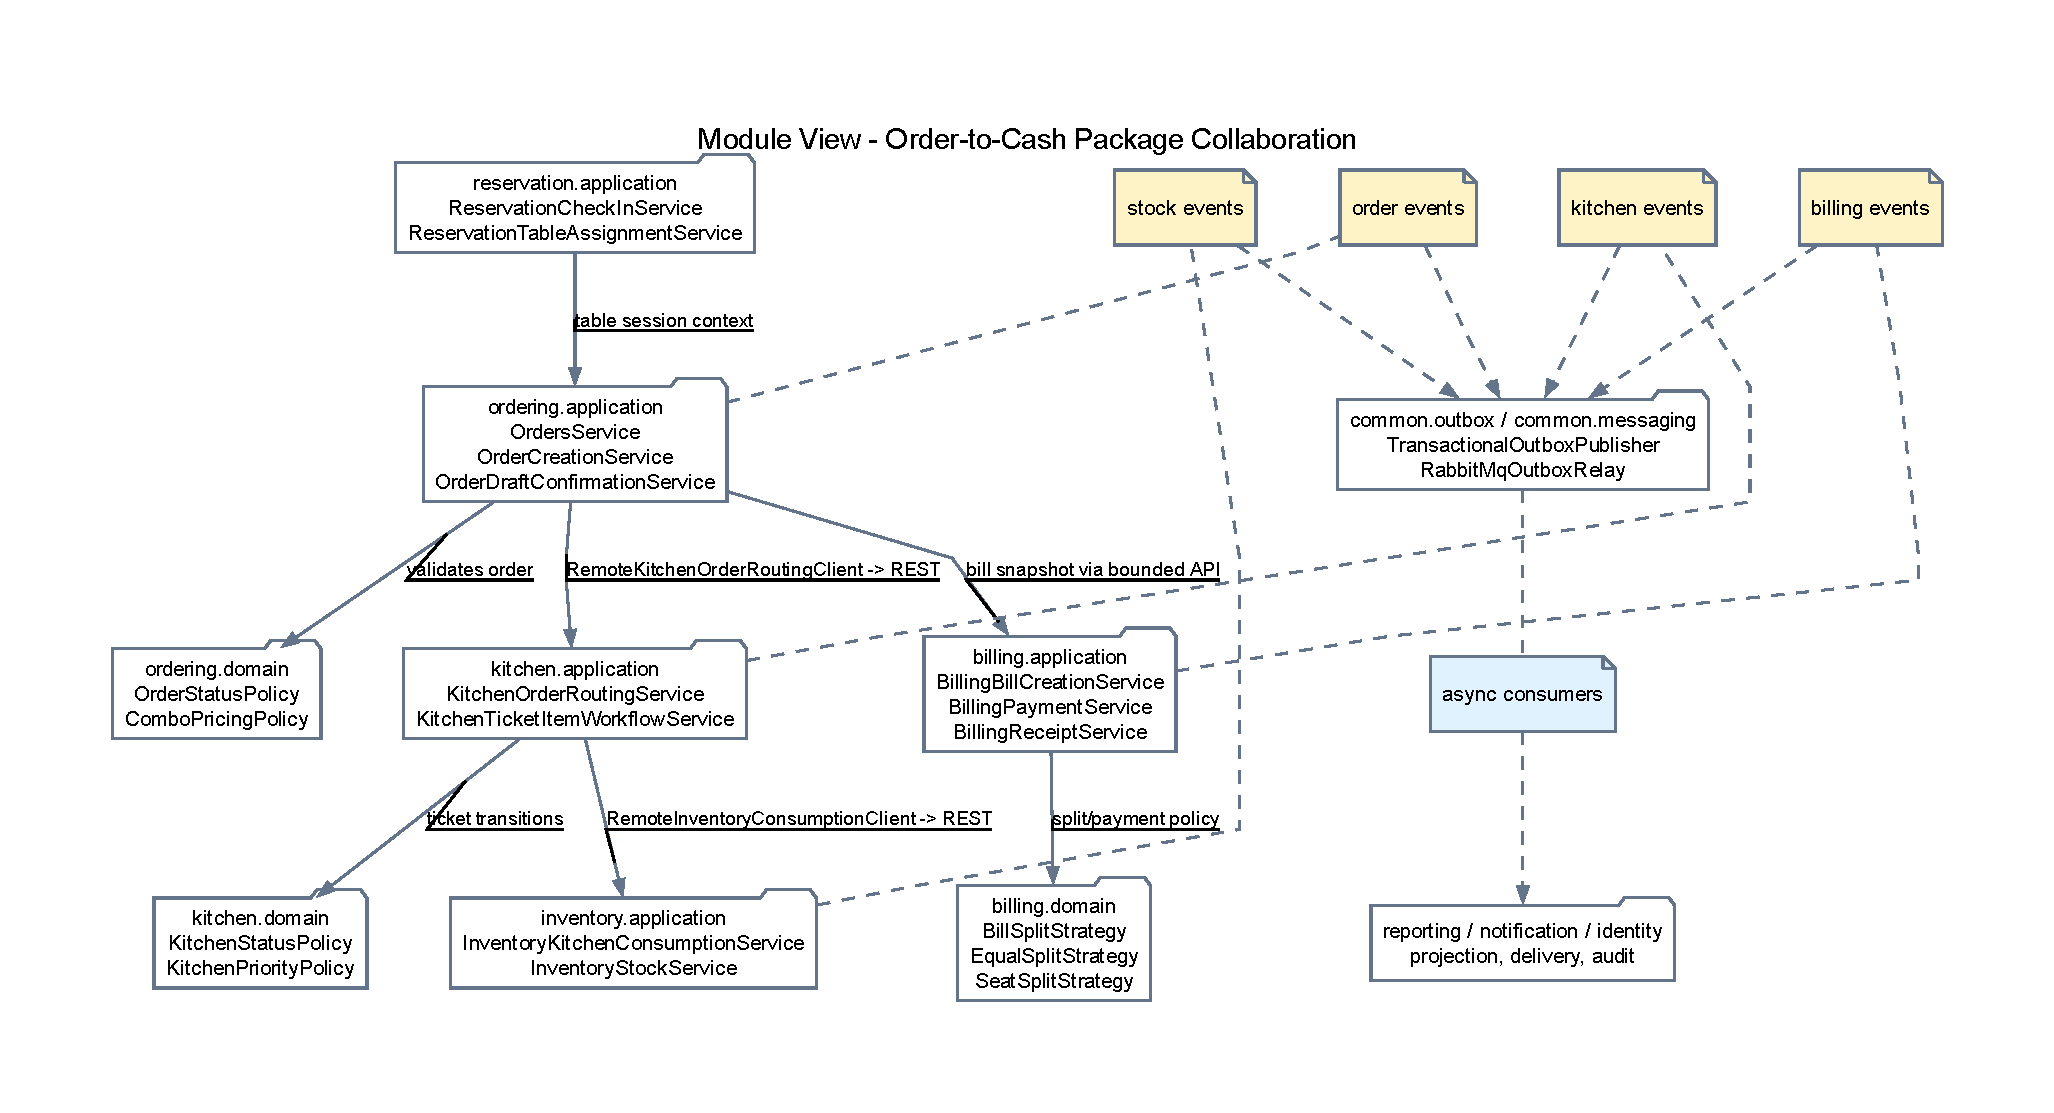
\includegraphics[width=\textwidth,height=0.84\textheight,keepaspectratio]{35_module_view_order_to_cash_slices.pdf}
}{
  \IfFileExists{35_module_view_order_to_cash_slices.png}{
    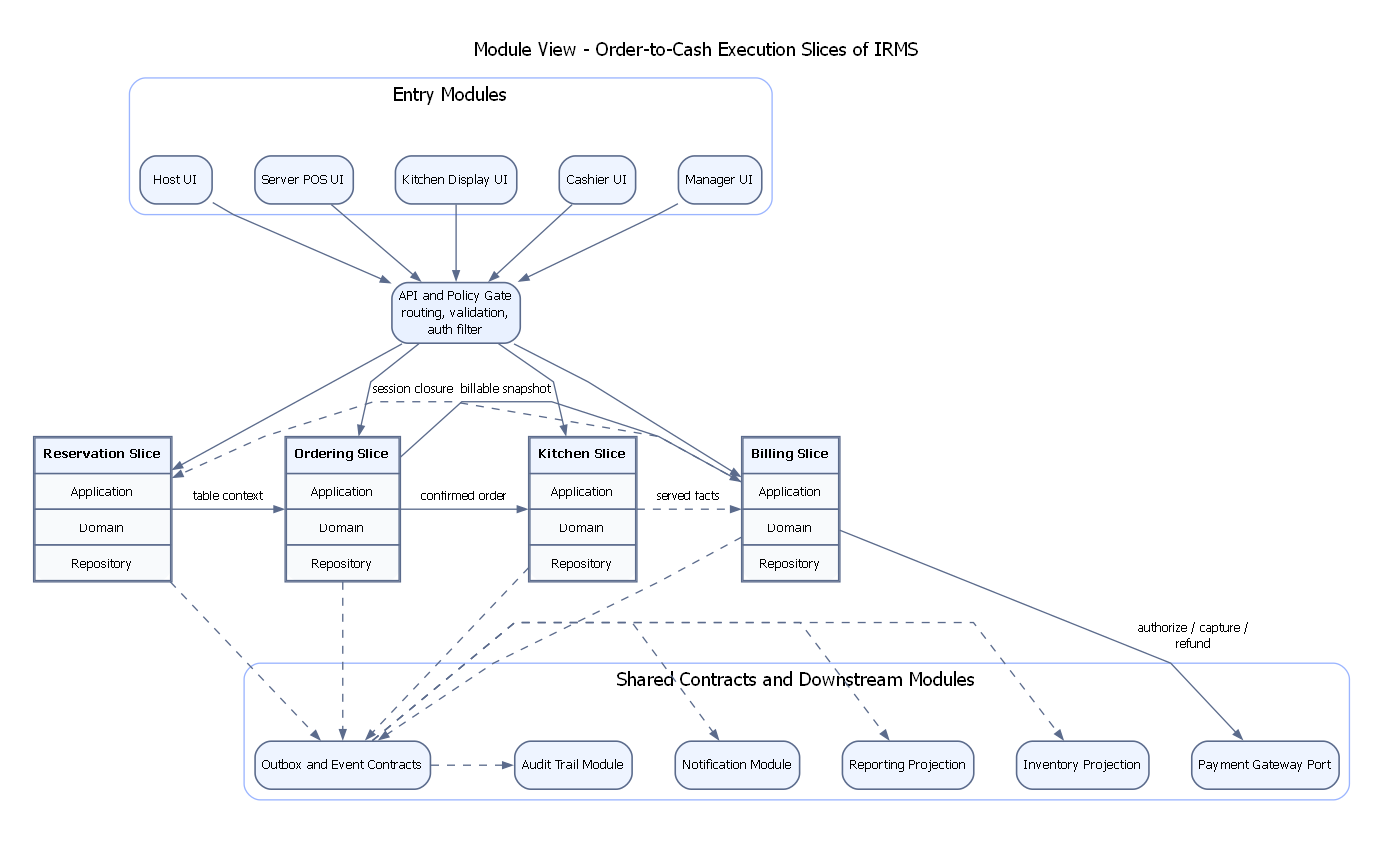
\includegraphics[width=\textwidth,height=0.84\textheight,keepaspectratio]{35_module_view_order_to_cash_slices.png}
  }{
    \fbox{\parbox{0.82\linewidth}{Thiếu file \textsf{35\_module\_view\_order\_to\_cash\_slices.(pdf/png)}.}}
  }
}
\caption{Module View chi tiết cho tuyến order-to-cash của IRMS}
\label{fig:irms-module-order-to-cash}
\end{figure}

Hình~\ref{fig:irms-module-order-to-cash} đi sâu vào luồng nghiệp vụ Order-to-Cash: từ lúc khách nhận bàn, gọi món, báo xuống bếp, thanh toán cho đến khi hệ thống phát sự kiện thông báo và cập nhật báo cáo. Dưới góc nhìn Module View cho riêng lát cắt nghiệp vụ này, sơ đồ tập trung làm rõ các package và class chính tham gia xử lý như \textsf{ReservationCheckInService}, \textsf{OrdersService}, \textsf{KitchenOrderRoutingService}, \textsf{BillingPaymentService} và \textsf{RabbitMqEventPublisher}.

Trong thiết kế này, \textbf{mỗi service sẽ tự quản lý lớp điều phối và các port hạ tầng của riêng nó}. Cụ thể, \textsf{ReservationSeatingMediator} lo việc nhận và xếp bàn; \textsf{OrdersService} xử lý tạo đơn; \textsf{RemoteKitchenOrderRoutingClient} sẽ giao tiếp với \textsf{KitchenIntegrationController}; tiến độ làm món được \textsf{KitchenTicketItemWorkflowService} theo dõi; còn \textsf{BillingPaymentService} thì kết nối qua interface \textsf{PaymentGateway}. Các service này hoạt động độc lập, chỉ phụ thuộc nhau qua API, event hoặc interface chứ không truy cập chéo vào cấu trúc nội bộ của nhau.

Sơ đồ cũng thể hiện rõ việc phân tách giữa \textbf{luồng xử lý đồng bộ} (synchronous) và \textbf{luồng xử lý bất đồng bộ qua event} (asynchronous). Các thao tác cần phản hồi cho user ngay lập tức (nhận bàn, chốt order, lập hóa đơn, thanh toán) sẽ được chạy đồng bộ. Ngược lại, các tác vụ "hậu cần" sẽ được đẩy vào \textsf{RabbitMqEventPublisher} để các consumer (\textsf{ReportingProjectionConsumer}, \textsf{NotificationRequestedConsumer}, \textsf{AuditRecordingRequestedConsumer}) tự động bắt lấy và xử lý. Việc tách bạch này giúp luồng chính chạy nhanh hơn và không bị block bởi các tác vụ phụ như gửi thông báo, lưu log audit hay tổng hợp báo cáo.

Cuối cùng, các controller và gateway đóng vai trò là các điểm chạm (entry point) đứng trước các service nghiệp vụ. Đây là nơi tiếp nhận request, validate dữ liệu và chuẩn hóa lời gọi. Nhờ có tầng biên này, các service nghiệp vụ bên trong không phải gánh thêm phần logic kỹ thuật, đồng thời đảm bảo ranh giới giao dịch (transaction boundary) của từng service được giữ nguyên vẹn.
\paragraph{Mô tả}
\begin{itemize}
  \item \textbf{Lát cắt service} được thể hiện bằng package và class thật: controller, service ứng dụng, interface và client tích hợp.
  \item \textbf{Tuyến phụ thuộc tĩnh} chỉ đi qua giao diện công khai và client REST cần thiết, nhờ đó tránh phụ thuộc chéo vào chi tiết nội bộ.
  \item \textbf{Tuyến hệ quả sự kiện} được tách sang \textsf{RabbitMqEventPublisher} và các bộ xử lý sự kiện nền, bảo vệ đường nóng khỏi tác vụ phụ.
  \item \textbf{PaymentGateway} là interface với hai hiện thực \textsf{CashPaymentGateway} và \textsf{ExternalReferencePaymentGateway}.
  \item \textbf{Quy tắc phụ thuộc runtime} ở hình này là cơ sở để kiểm chứng phần hiện thực hiện thực: nếu service truy cập xuyên qua chi tiết nội bộ của nhau, kiến trúc sẽ bị phá vỡ ngay ở mức thiết kế.
\end{itemize}


\subsection{Góc nhìn thành phần và kết nối}\label{sec:component-connector-view}

Góc nhìn này cụ thể hóa các quyết định về gateway boundary, REST đồng bộ, event-driven processing, outbox, RabbitMQ và idempotency trong \adrref{ADR-0003}{adr:0003-gateway-boundary}, \adrref{ADR-0004}{adr:0004-rest-sync}, \adrref{ADR-0005}{adr:0005-event-driven}, \adrref{ADR-0006}{adr:0006-outbox}, \adrref{ADR-0007}{adr:0007-rabbitmq} và \adrref{ADR-0010}{adr:0010-idempotency}.
Ở góc nhìn thành phần và kết nối, hệ thống được mô tả bằng các thành phần thực thi chính và các kiểu liên kết giữa chúng. Góc nhìn này đặc biệt quan trọng vì nó cho biết một yêu cầu đi qua những khối nào, khối nào giữ quyết định nghiệp vụ và khối nào chỉ đóng vai trò tích hợp hoặc hỗ trợ kỹ thuật.

\subsubsection{Các thành phần chính}\label{sec:main-components}
Góc nhìn này bóc tách hệ thống thành các khối thực thi cụ thể, đảm bảo sự phân tách rạch ròi giữa trải nghiệm giao diện, điều phối luồng, luật nghiệp vụ và tích hợp hạ tầng phần cứng lẫn phần mềm:

\begin{itemize}
  \item \textbf{Các ứng dụng giao diện (Client Applications):} Gồm giao diện cho lễ tân, phục vụ, bếp, thu ngân và quản lý. Lớp này tiếp nhận thao tác người dùng, gọi các endpoint trong \textsf{ENDPOINTS} của frontend và hiển thị lại dữ liệu do backend trả về:
  \begin{itemize}
      \item Dùng \textsf{apiFetch} và \textsf{ENDPOINTS} để gọi REST API qua \textsf{Nitro API Proxy}.
      \item Dùng \textsf{permissions.ts} và dữ liệu vai trò từ \textsf{/api/auth/me} để kiểm soát điều hướng theo quyền trên giao diện.
  \end{itemize}

  \item \textbf{Cổng vào hệ thống (API Gateway \& Frontend Proxy):} \textsf{Frontend Node Server} phục vụ React và chuyển tiếp \textsf{/api}; \textsf{GatewayProxyController} trong \textsf{api-gateway} định tuyến yêu cầu REST đến các service phía sau. Thiết kế hiện tại chưa cho thấy WebSocket/SSE, rate limiting hay cấu hình Nginx riêng.

  \item \textbf{Các dịch vụ ứng dụng (Application Services):} Lớp này chịu trách nhiệm điều phối các use case. Thành phần này không chứa luật nghiệp vụ mà chỉ quản lý ranh giới giao dịch, gọi các đối tượng miền phù hợp và ủy quyền việc phát sự kiện.

  \item \textbf{Các service miền nghiệp vụ (Domain Services):} Đây là lớp lõi của kiến trúc, chứa các Aggregate Roots và các bất biến nghiệp vụ. Mọi quyết định nghiệp vụ như tính tiền hoặc xác định trạng thái bàn chỉ được xử lý tại lớp này.

  \item \textbf{Lớp lưu trữ dữ liệu (Data Persistence):} Thực hiện lưu trữ thông qua mẫu Repository nhằm cô lập nghiệp vụ khỏi nền tảng SQL. Lớp này phân tách rõ giữa \textbf{Mô hình ghi (Transactional Schema)} phục vụ cho tốc độ giao dịch nóng và \textbf{Mô hình đọc (Reporting Projections)} phục vụ truy vấn phân tích để không gây nghẽn cổ chai cơ sở dữ liệu.

  \item \textbf{Bộ truyền sự kiện và xử lý nền (Event Bus \& Background Workers):} Đảm bảo tính nhất quán cuối cùng (Eventual Consistency) của hệ thống. Hệ thống áp dụng \textbf{Outbox Pattern} với \textbf{Outbox Dispatcher} để quét và đẩy sự kiện một cách đáng tin cậy. Các hệ quả bất đồng bộ (như cập nhật kho, gửi thông báo) được đưa vào hàng đợi nền để không làm chậm luồng thao tác trực tiếp của nhân viên.

  \item \textbf{Các bộ kết nối thích nghi (Adapters):} Được thiết kế theo nguyên lý Đảo ngược phụ thuộc (Dependency Inversion), chia làm hai nhóm đã thấy trong thiết kế nhằm cách ly lõi nghiệp vụ:
  \begin{itemize}
      \item \textit{Bộ kết nối thanh toán}: \textsf{CashPaymentGateway} và \textsf{ExternalReferencePaymentGateway} hiện thực interface \textsf{PaymentGateway}.
      \item \textit{Bộ kết nối thông báo và biên lai}: \textsf{EmailNotificationChannelAdapter}, \textsf{SmsNotificationChannelAdapter}, \textsf{InAppNotificationChannelAdapter}, \textsf{PrintNotificationChannelAdapter}, \textsf{PrintReceiptDeliveryAdapter} và \textsf{DigitalReceiptDeliveryAdapter}.
  \end{itemize}
\end{itemize}

\subsubsection{Các kiểu kết nối chính}\label{sec:main-connectors}
Để đáp ứng yêu cầu về hiệu năng cao và tính nhất quán của dữ liệu trong môi trường vận hành nhà hàng, IRMS kết hợp các kiểu kết nối đã có trong thiết kế và cấu hình. Các tương tác giữa các thành phần được định nghĩa qua bảng sau:

\begin{table}[H]
\centering
\caption{Các kiểu kết nối chính trong IRMS}
\begin{tabularx}{\textwidth}{|p{2.95cm}|X|p{4cm}|}
\hline
\textbf{Kiểu kết nối} & \textbf{Vai trò và Đặc tính kỹ thuật} & \textbf{Ví dụ thực tế trong IRMS} \\
\hline
Giao thức HTTP (REST API) & Kết nối đồng bộ (Synchronous), ưu tiên độ trễ thấp và phản hồi trạng thái giao dịch tức thì. & POS App gửi yêu cầu xác nhận đơn gọi món hoặc lập hóa đơn. \\
\hline
REST qua \textsf{apiFetch} & Frontend gọi định kỳ hoặc gọi lại sau thao tác người dùng để tải trạng thái mới. & Màn hình bếp gọi \textsf{/api/kitchen/overview}; màn hình báo cáo gọi các endpoint trong \textsf{/api/reports}. \\
\hline
Thông điệp Sự kiện (Pub/Sub) & Kết nối bất đồng bộ (Asynchronous) qua Message Broker, giúp giảm sự phụ thuộc trực tiếp (Decoupling) giữa các module. & Lan truyền sự kiện đơn hàng hoàn tất để trừ tồn kho và làm giàu dữ liệu báo cáo. \\
\hline  
Adapter nội bộ & Interface và adapter trong thiết kế để cô lập biến thể nghiệp vụ hoặc kênh phát hành. & \textsf{PaymentGateway}, \textsf{NotificationChannelAdapter} và \textsf{ReceiptDeliveryAdapter}. \\
\hline
Kết nối Database (JDBC / Driver) & Truy xuất dữ liệu có cấu trúc và quản lý ranh giới giao dịch (Atomic Transactions). & Business Services lưu trữ trạng thái bàn và phiên phục vụ vào PostgreSQL. \\
\hline
\end{tabularx}
\end{table}

\subsubsection{Cơ sở lựa chọn mô hình kết nối hỗn hợp}\label{sec:connector-rationale}
Kiến trúc IRMS không sử dụng duy nhất một kiểu kết nối mà kết hợp linh hoạt dựa trên hai nguyên tắc cốt lõi:

\begin{enumerate}
    \item \textbf{Tuyến đầu ưu tiên đồng bộ (Sync for UX):} Các thao tác tương tác trực tiếp với khách hàng (đặt bàn, gọi món, thanh toán) được thực hiện qua API đồng bộ. Điều này giúp nhân viên nhận được phản hồi "Thành công" hoặc "Thất bại" ngay lập tức, đảm bảo luồng phục vụ không bị gián đoạn.
    
    \item \textbf{Hậu phương ưu tiên bất đồng bộ (Async for Resilience):} Các hệ quả phát sinh sau giao dịch như gửi thông báo, cập nhật kho, audit và tổng hợp báo cáo được đẩy sang tuyến sự kiện qua \textsf{RabbitMQ}, \textsf{outbox\_events} và các bộ xử lý nền. Việc này giúp bảo vệ hệ thống: nếu một tác vụ phụ bị chậm hoặc lỗi, nó cũng không làm nghẽn luồng nghiệp vụ chính.
\end{enumerate}


\textbf{Góc nhìn chuyên sâu về thành phần và kết nối:} \\
Điểm then chốt trong kiến trúc IRMS là sự phân định rạch ròi giữa \emph{kết nối phục vụ trải nghiệm người dùng} và \emph{kết nối phục vụ phối hợp nội bộ}. Việc chọn đúng chiến lược giao tiếp cho từng ngữ cảnh không chỉ quyết định độ trễ phản hồi mà còn ảnh hưởng trực tiếp đến khả năng chịu lỗi (fault tolerance) và tính mở rộng của toàn hệ thống.



\begin{figure}[H]
\centering
\IfFileExists{09_component_and_connector_view_overall_runtime_structure.pdf}{
  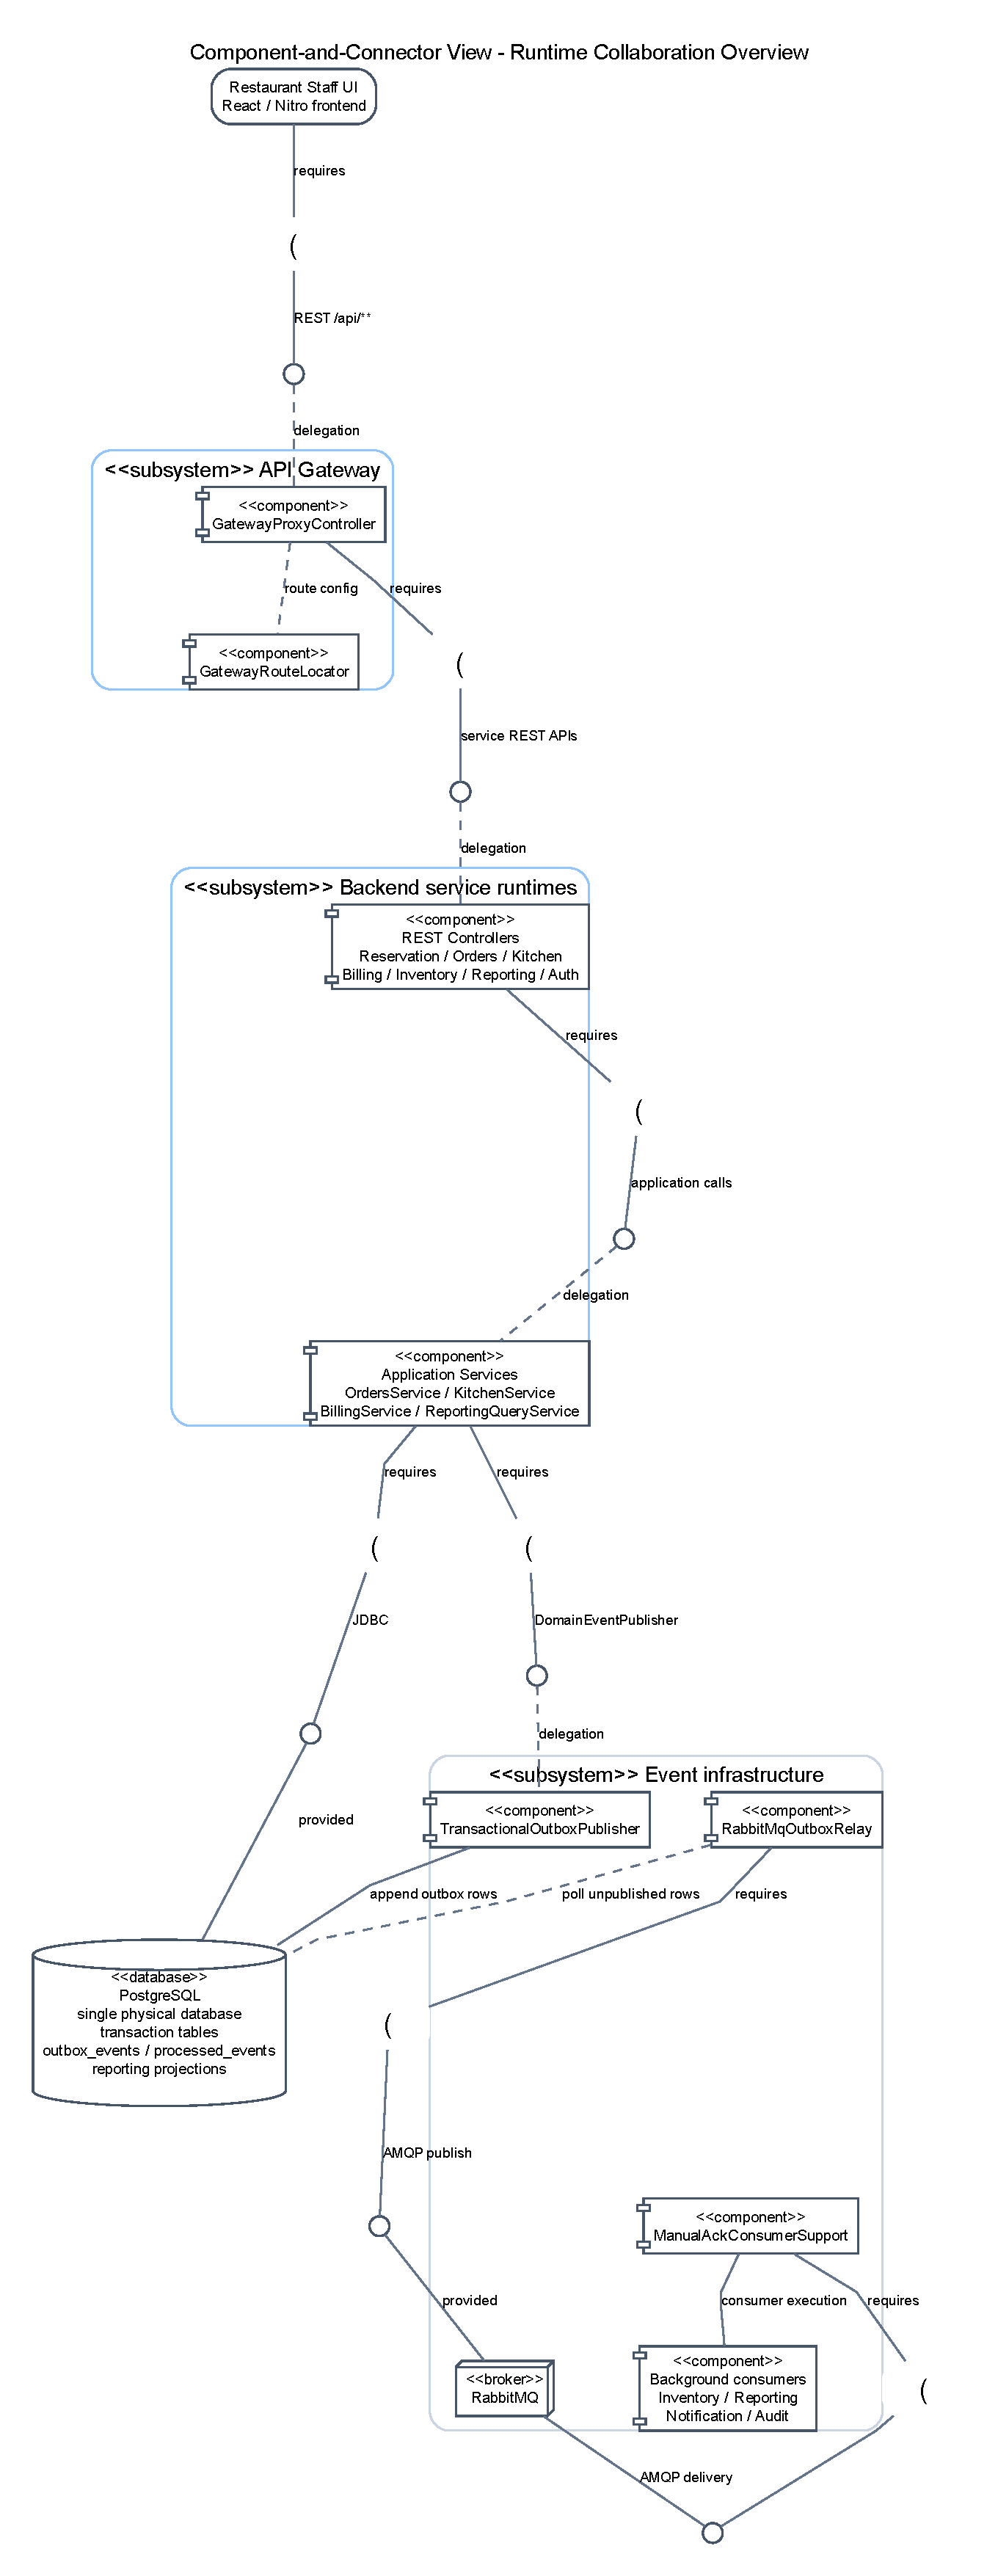
\includegraphics[width=0.97\linewidth,height=0.84\textheight,keepaspectratio]{09_component_and_connector_view_overall_runtime_structure.pdf}
}{
  \IfFileExists{09_component_and_connector_view_overall_runtime_structure.png}{
    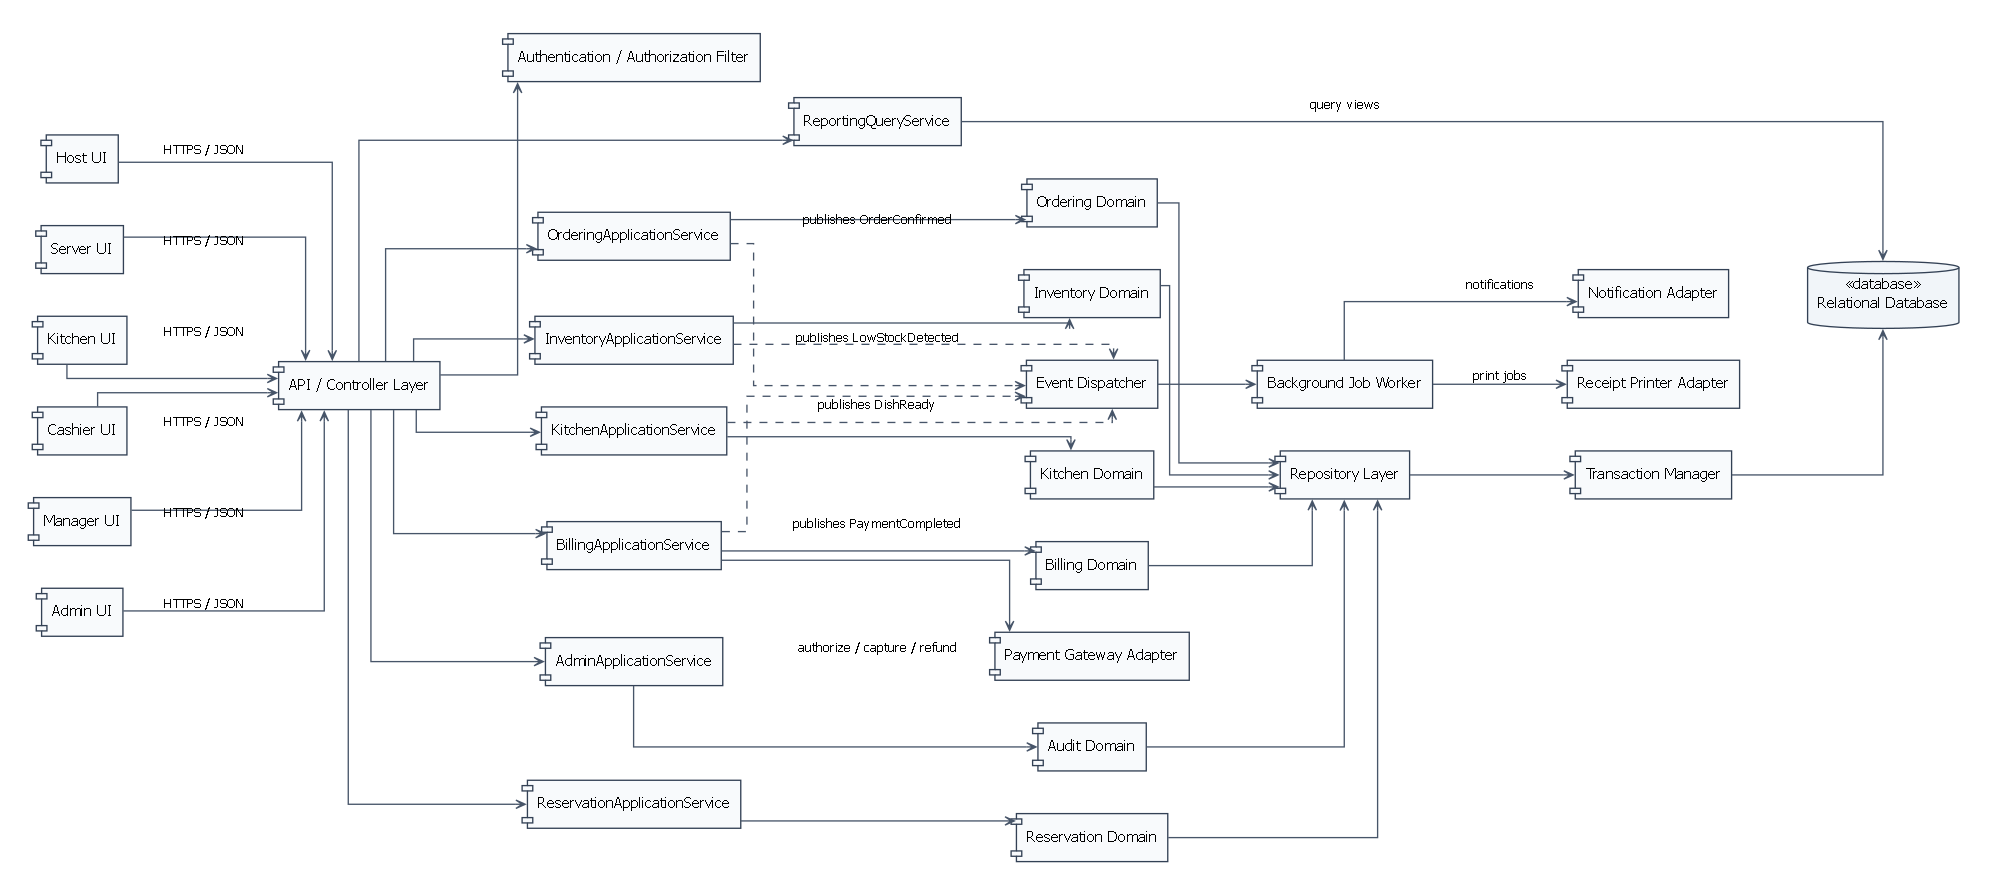
\includegraphics[width=0.97\linewidth,height=0.84\textheight,keepaspectratio]{09_component_and_connector_view_overall_runtime_structure.png}
  }{
    \fbox{\parbox{0.82\linewidth}{Thiếu file \textsf{09\_component\_and\_connector\_view\_overall\_runtime\_structure.(pdf/png)}.}}
  }
}
\caption{Sơ đồ thành phần và kết nối tổng quan của IRMS}
\label{fig:irms-cc-overall}
\end{figure}



Hình~\ref{fig:irms-cc-overall} thể hiện cấu trúc thực thi tổng quan của hệ thống theo cách nhìn thành phần. Thiết bị người dùng chỉ giao tiếp với lớp cổng vào; từ đó yêu cầu đi qua lớp điều phối ca sử dụng, xuống miền nghiệp vụ, lớp lưu trữ và các adapter biên. Ý nghĩa học thuật của hình này là làm rõ hệ thống không được tổ chức như một khối gọi chéo tùy ý, mà có hướng phụ thuộc rõ ràng từ ngoài vào trong.

\paragraph{Các thành phần chính}
\begin{itemize}
  \item \textbf{Các ứng dụng giao diện}: là nơi phát sinh yêu cầu từ lễ tân, phục vụ, bếp, thu ngân và quản lý.
  \item \textbf{Cổng vào giao diện lập trình ứng dụng}: tiếp nhận yêu cầu, xác thực, kiểm tra đầu vào và chuyển tiếp tới đúng ca sử dụng.
  \item \textbf{Các dịch vụ ứng dụng}: điều phối từng ca sử dụng cụ thể như tạo đặt bàn, xác nhận đơn gọi món, cập nhật phiếu bếp hoặc chốt hóa đơn.
  \item \textbf{Các service miền nghiệp vụ}: giữ luật nghiệp vụ cốt lõi, bất biến dữ liệu và quyết định nghiệp vụ của nhà hàng.
  \item \textbf{Lớp lưu trữ dữ liệu}: chịu trách nhiệm lưu trữ trạng thái giao dịch và bảo vệ ranh giới giao dịch.
  \item \textbf{Bộ phát sự kiện và bộ xử lý nền}: xử lý sự kiện và tác vụ nền không nên nằm trên tuyến giao dịch nóng.
  \item \textbf{Các port/adapter biên}: bao bọc cách xử lý thanh toán, gửi thông báo và phát hành biên lai.
\end{itemize}


\begin{figure}[H]
\centering
\IfFileExists{10_component_diagram_detailed_backend_composition.pdf}{
  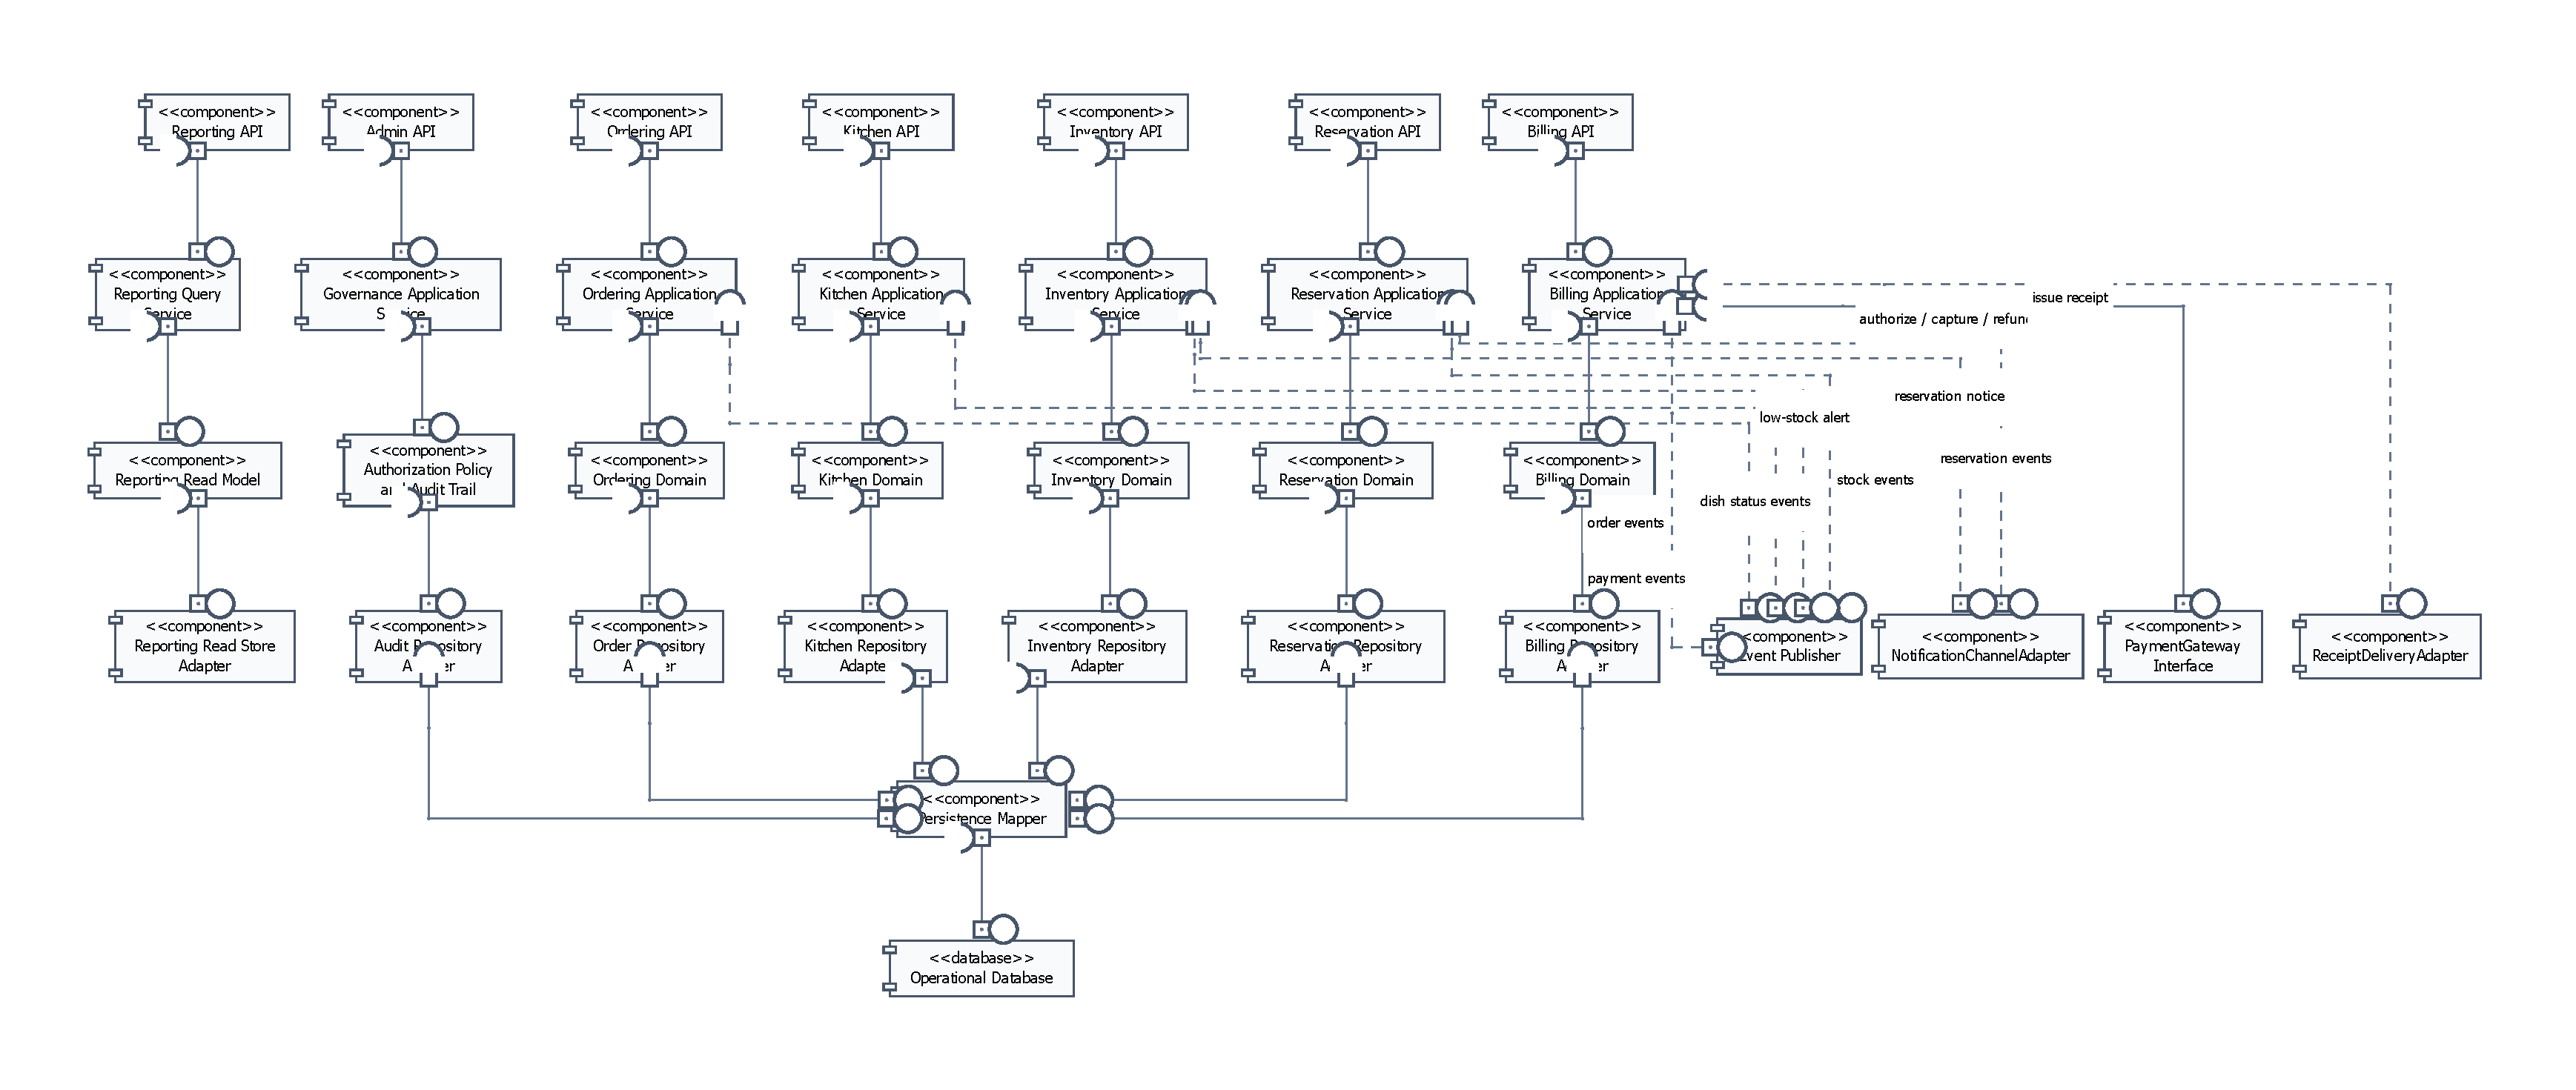
\includegraphics[width=0.97\linewidth,height=0.84\textheight,keepaspectratio]{10_component_diagram_detailed_backend_composition.pdf}
}{
  \IfFileExists{10_component_diagram_detailed_backend_composition.png}{
    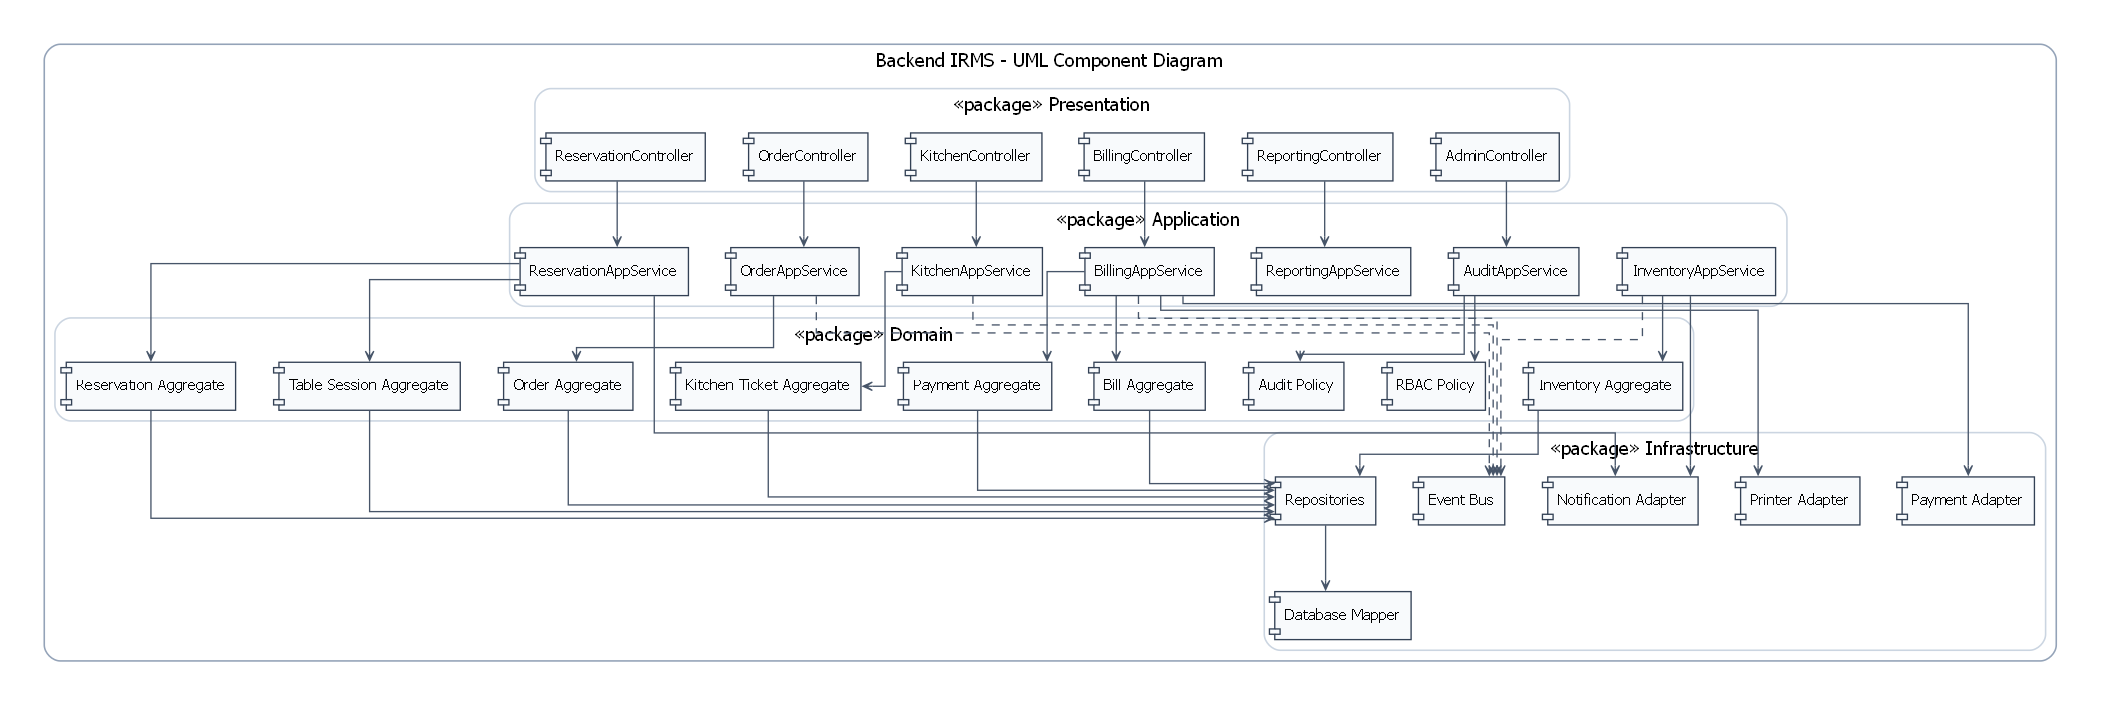
\includegraphics[width=0.97\linewidth,height=0.84\textheight,keepaspectratio]{10_component_diagram_detailed_backend_composition.png}
  }{
    \fbox{\parbox{0.82\linewidth}{Thiếu file \textsf{10\_component\_diagram\_detailed\_backend\_composition.(pdf/png)}.}}
  }
}
\caption{Sơ đồ thành phần chi tiết của lớp service nghiệp vụ trong IRMS}
\label{fig:irms-cc-backend}
\end{figure}



Hình~\ref{fig:irms-cc-backend} mở chi tiết lớp backend ở mức component, nhưng không trộn sang Class Diagram. Sơ đồ gom các controller REST, application service, required interface và provided adapter theo đúng vai trò trong thiết kế. Nhờ đó người đọc thấy rõ yêu cầu đi từ biên API vào lớp điều phối, sau đó phụ thuộc vào các port như repository, \textsf{PaymentGateway}, \textsf{ReceiptDeliveryAdapter}, \textsf{SharedIdentity*Port} và \textsf{DomainEventPublisher}.

Điểm chính của hình là hướng phụ thuộc được kiểm soát qua interface. Các application service không phụ thuộc trực tiếp vào JDBC adapter, gateway thanh toán hay cơ chế outbox cụ thể; những thành phần đó cung cấp lại năng lực qua adapter ở rìa. Cách biểu diễn này khớp với thiết kế hiện tại, nơi các lớp như \textsf{JdbcOrderRepository}, \textsf{CashPaymentGateway}, \textsf{ExternalReferencePaymentGateway}, \textsf{RemoteSharedIdentity*Client} và \textsf{TransactionalOutboxPublisher} nằm ở phía hiện thực kỹ thuật.

\paragraph{Các thành phần chính}
\begin{itemize}
  \item \textbf{API layer}: gom các controller REST của những module nghiệp vụ chính.
  \item \textbf{Application services}: gom các service điều phối use case như \textsf{OrdersService}, \textsf{KitchenService}, \textsf{BillingService}, \textsf{ReservationService}, \textsf{InventoryService}, \textsf{ReportingQueryService}, \textsf{AuthService} và \textsf{AuditService}.
  \item \textbf{Required interfaces}: mô tả các port mà lớp ứng dụng cần, gồm port truy cập dữ liệu, integration port và event publisher.
  \item \textbf{Provided adapters}: mô tả các adapter cung cấp các port trên, gồm JDBC adapter, payment/receipt adapter, shared identity client và outbox publisher.
\end{itemize}



\subsubsection{Sơ đồ thành phần cho tuyến lệnh vận hành}


\begin{figure}[H]
\centering
\IfFileExists{24_component_diagram_operational_command_collaboration.pdf}{
  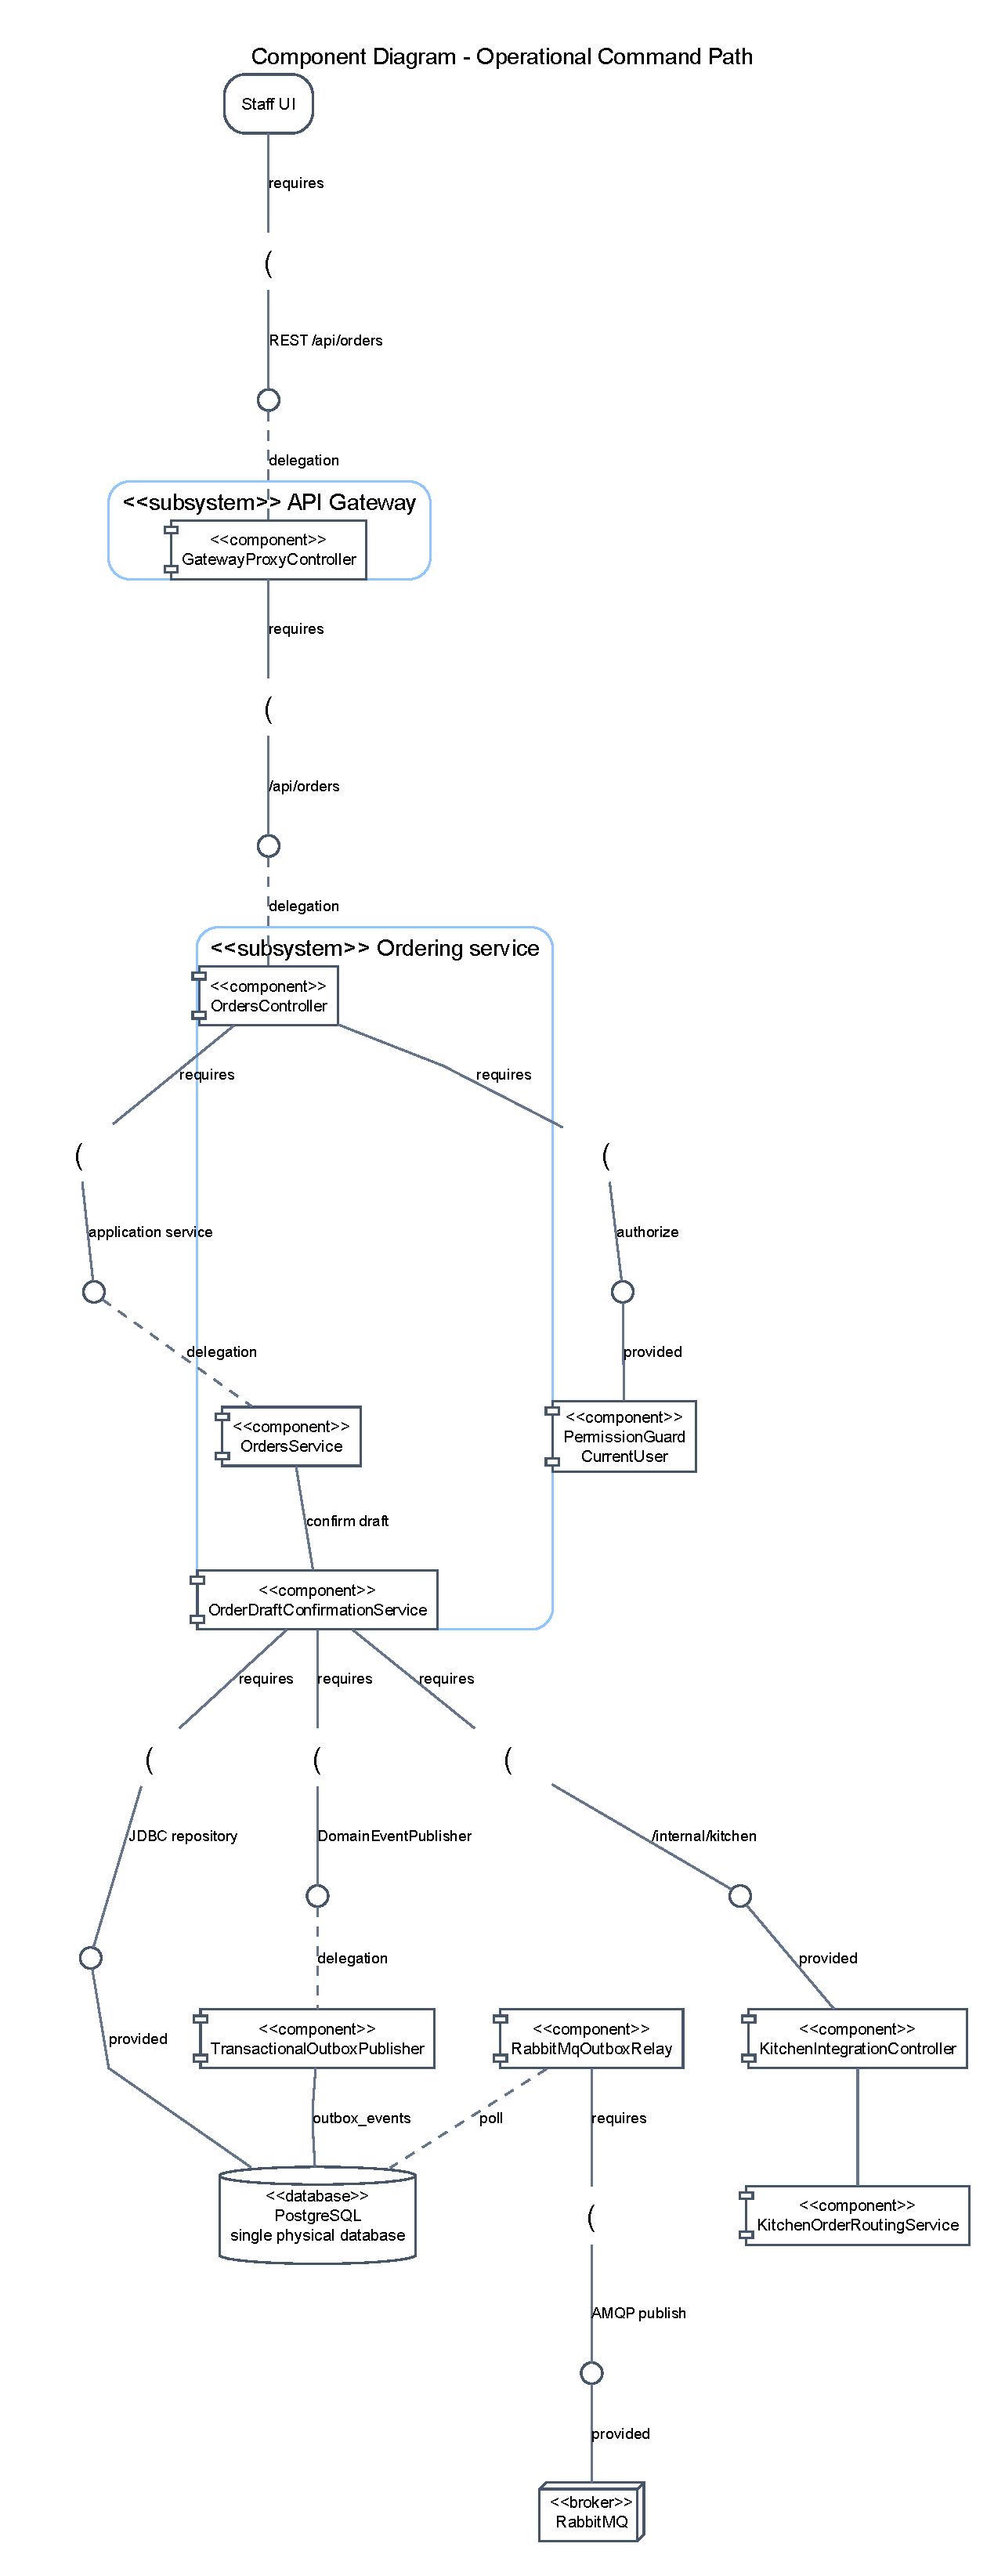
\includegraphics[width=0.97\linewidth,height=0.84\textheight,keepaspectratio]{24_component_diagram_operational_command_collaboration.pdf}
}{
  \IfFileExists{24_component_diagram_operational_command_collaboration.png}{
    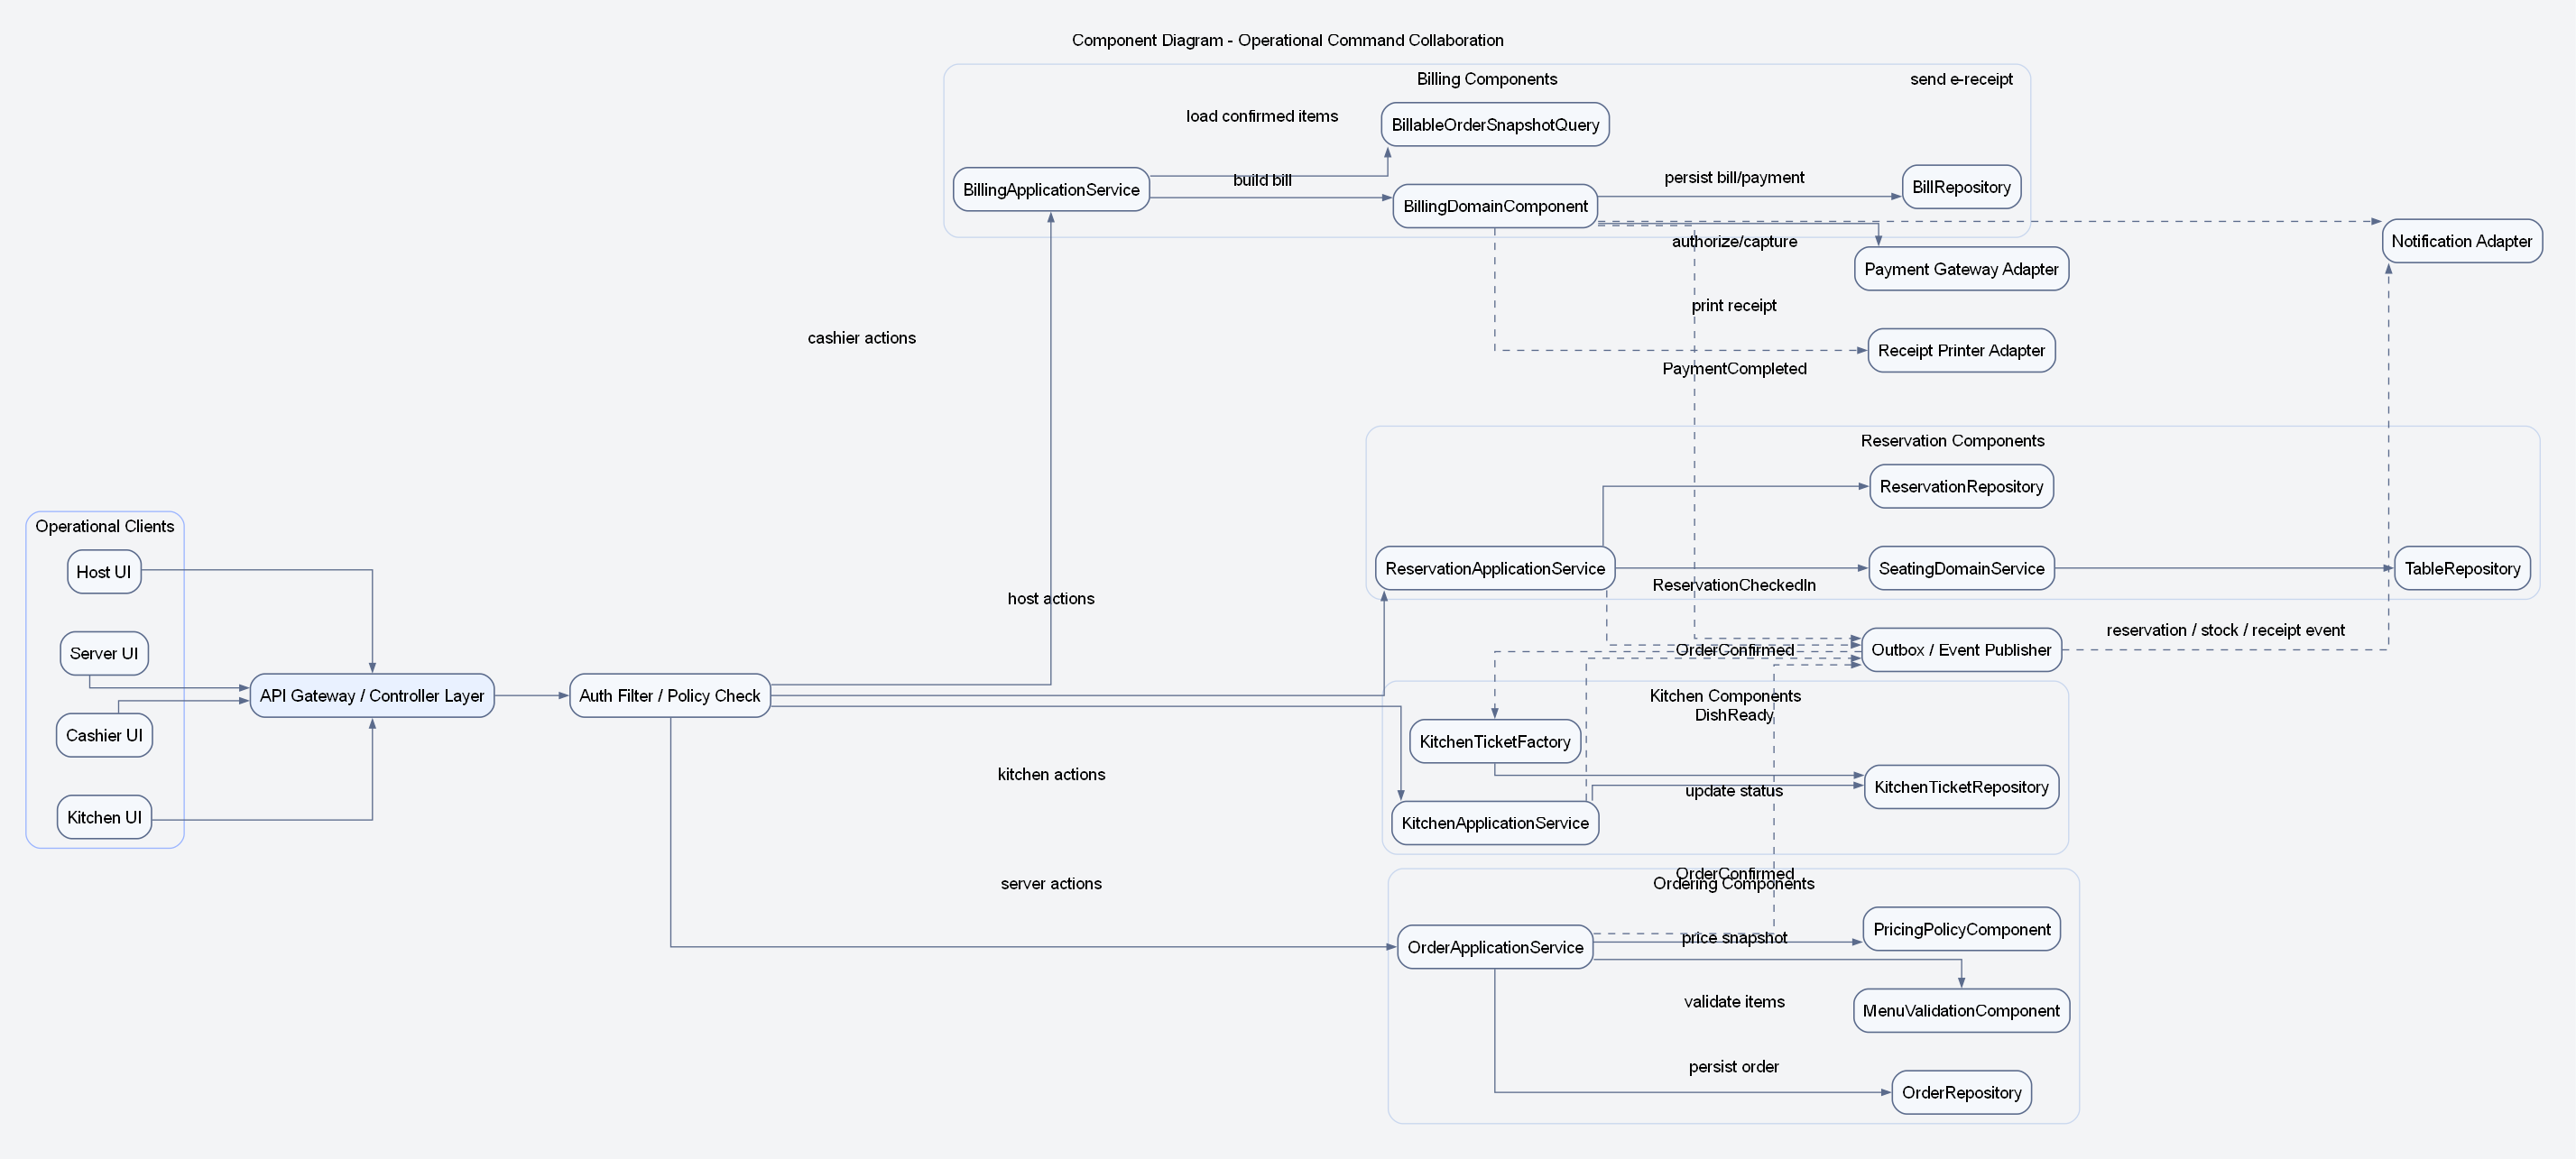
\includegraphics[width=0.97\linewidth,height=0.84\textheight,keepaspectratio]{24_component_diagram_operational_command_collaboration.png}
  }{
    \fbox{\parbox{0.8\linewidth}{Thiếu file \textsf{24\_component\_diagram\_operational\_command\_collaboration.(pdf/png)}.}}
  }
}
\caption{Sơ đồ thành phần cho tuyến lệnh vận hành của IRMS}
\label{fig:irms-component-operational-command}
\end{figure}



Hình~\ref{fig:irms-component-operational-command} mô tả luồng thực thi của một lệnh vận hành (operational command), từ giao diện người dùng đến khi dữ liệu được lưu trữ và các tác vụ phụ (side-effects) được kích hoạt. Trình tự này được thiết kế chặt chẽ để đảm bảo hệ thống hoạt động ổn định và có khả năng truy vết (audit).

Đầu tiên, các yêu cầu đi qua bộ lọc xác thực và phân quyền ở tầng biên (edge) để kiểm tra tính hợp lệ trước khi chạm vào hệ thống lõi. Sau đó, request được chuyển đến các Application Service (\textsf{Reservation}, \textsf{Ordering}, \textsf{Kitchen}, \textsf{Billing}). Tại đây, Application Service chỉ đóng vai trò điều phối (orchestration): gọi các đối tượng Domain tương ứng, quản lý vòng đời giao dịch (transaction), và ghi sự kiện vào Outbox (Outbox Pattern) để chuẩn bị cho các tác vụ tiếp theo.

Thứ hai, thiết kế tách biệt rõ ràng giữa \textbf{giao dịch lõi} (core transaction) và \textbf{tác vụ phụ} (side-effects). Các giao dịch chính (như chốt đơn, ghi nhận thanh toán) bắt buộc phải được commit thành công vào cơ sở dữ liệu. Chỉ khi trạng thái lõi đã nhất quán, hệ thống mới phát sự kiện (event) để xử lý các tác vụ bất đồng bộ như báo xuống bếp, gửi thông báo hoặc cập nhật Read Model. Cơ chế này thực thi nguyên tắc \enquote{lõi đồng bộ, hỗ trợ bất đồng bộ}, giúp tối ưu thời gian phản hồi cho client nhưng vẫn đảm bảo toàn vẹn dữ liệu.

Cuối cùng, việc đặt \textsf{PaymentGateway}, \textsf{ReceiptDeliveryAdapter} và \textsf{NotificationChannelAdapter} ở rìa kiến trúc thể hiện rõ việc áp dụng mô hình Ports \& Adapters. Tầng Domain chỉ định nghĩa các interface (Port), trong khi chi tiết tích hợp cụ thể với nhà cung cấp thanh toán hay máy in biên lai được giao cho các Adapter bên ngoài. Cách tổ chức này giúp lõi nghiệp vụ độc lập hoàn toàn với chi tiết hạ tầng.
\paragraph{Các thành phần chính}
\begin{itemize}
  \item \textbf{Cổng vào giao diện lập trình ứng dụng và lớp bộ điều khiển} cùng \textbf{bộ lọc xác thực / kiểm tra chính sách}: tiếp nhận yêu cầu, chuẩn hóa dữ liệu vào, xác thực và chặn hành vi vượt quyền trước khi đi vào lõi.
  \item \textbf{Các dịch vụ ứng dụng} của từng vùng \textsf{Reservation}, \textsf{Ordering}, \textsf{Kitchen} và \textsf{Billing}: điều phối use case, gọi đúng thành phần miền nghiệp vụ và kiểm soát biên giao dịch.
  \item \textbf{Các thành phần miền nghiệp vụ} và \textbf{kho lưu trữ}: hiện thực quy tắc miền và nơi lưu trạng thái bền vững.
  \item \textbf{Hộp thư ra / bộ phát sự kiện} cùng các port/adapter như \textsf{PaymentGateway}, \textsf{ReceiptDeliveryAdapter} và \textsf{NotificationChannelAdapter}: tách bước chốt giao dịch khỏi bước xử lý biên hoặc xử lý nền.
\end{itemize}


\subsubsection{Sơ đồ thành phần cho xử lý nền, quản trị và mô hình đọc}
\begin{figure}[H]
\centering
\IfFileExists{25_component_diagram_supporting_async_and_governance.pdf}{
  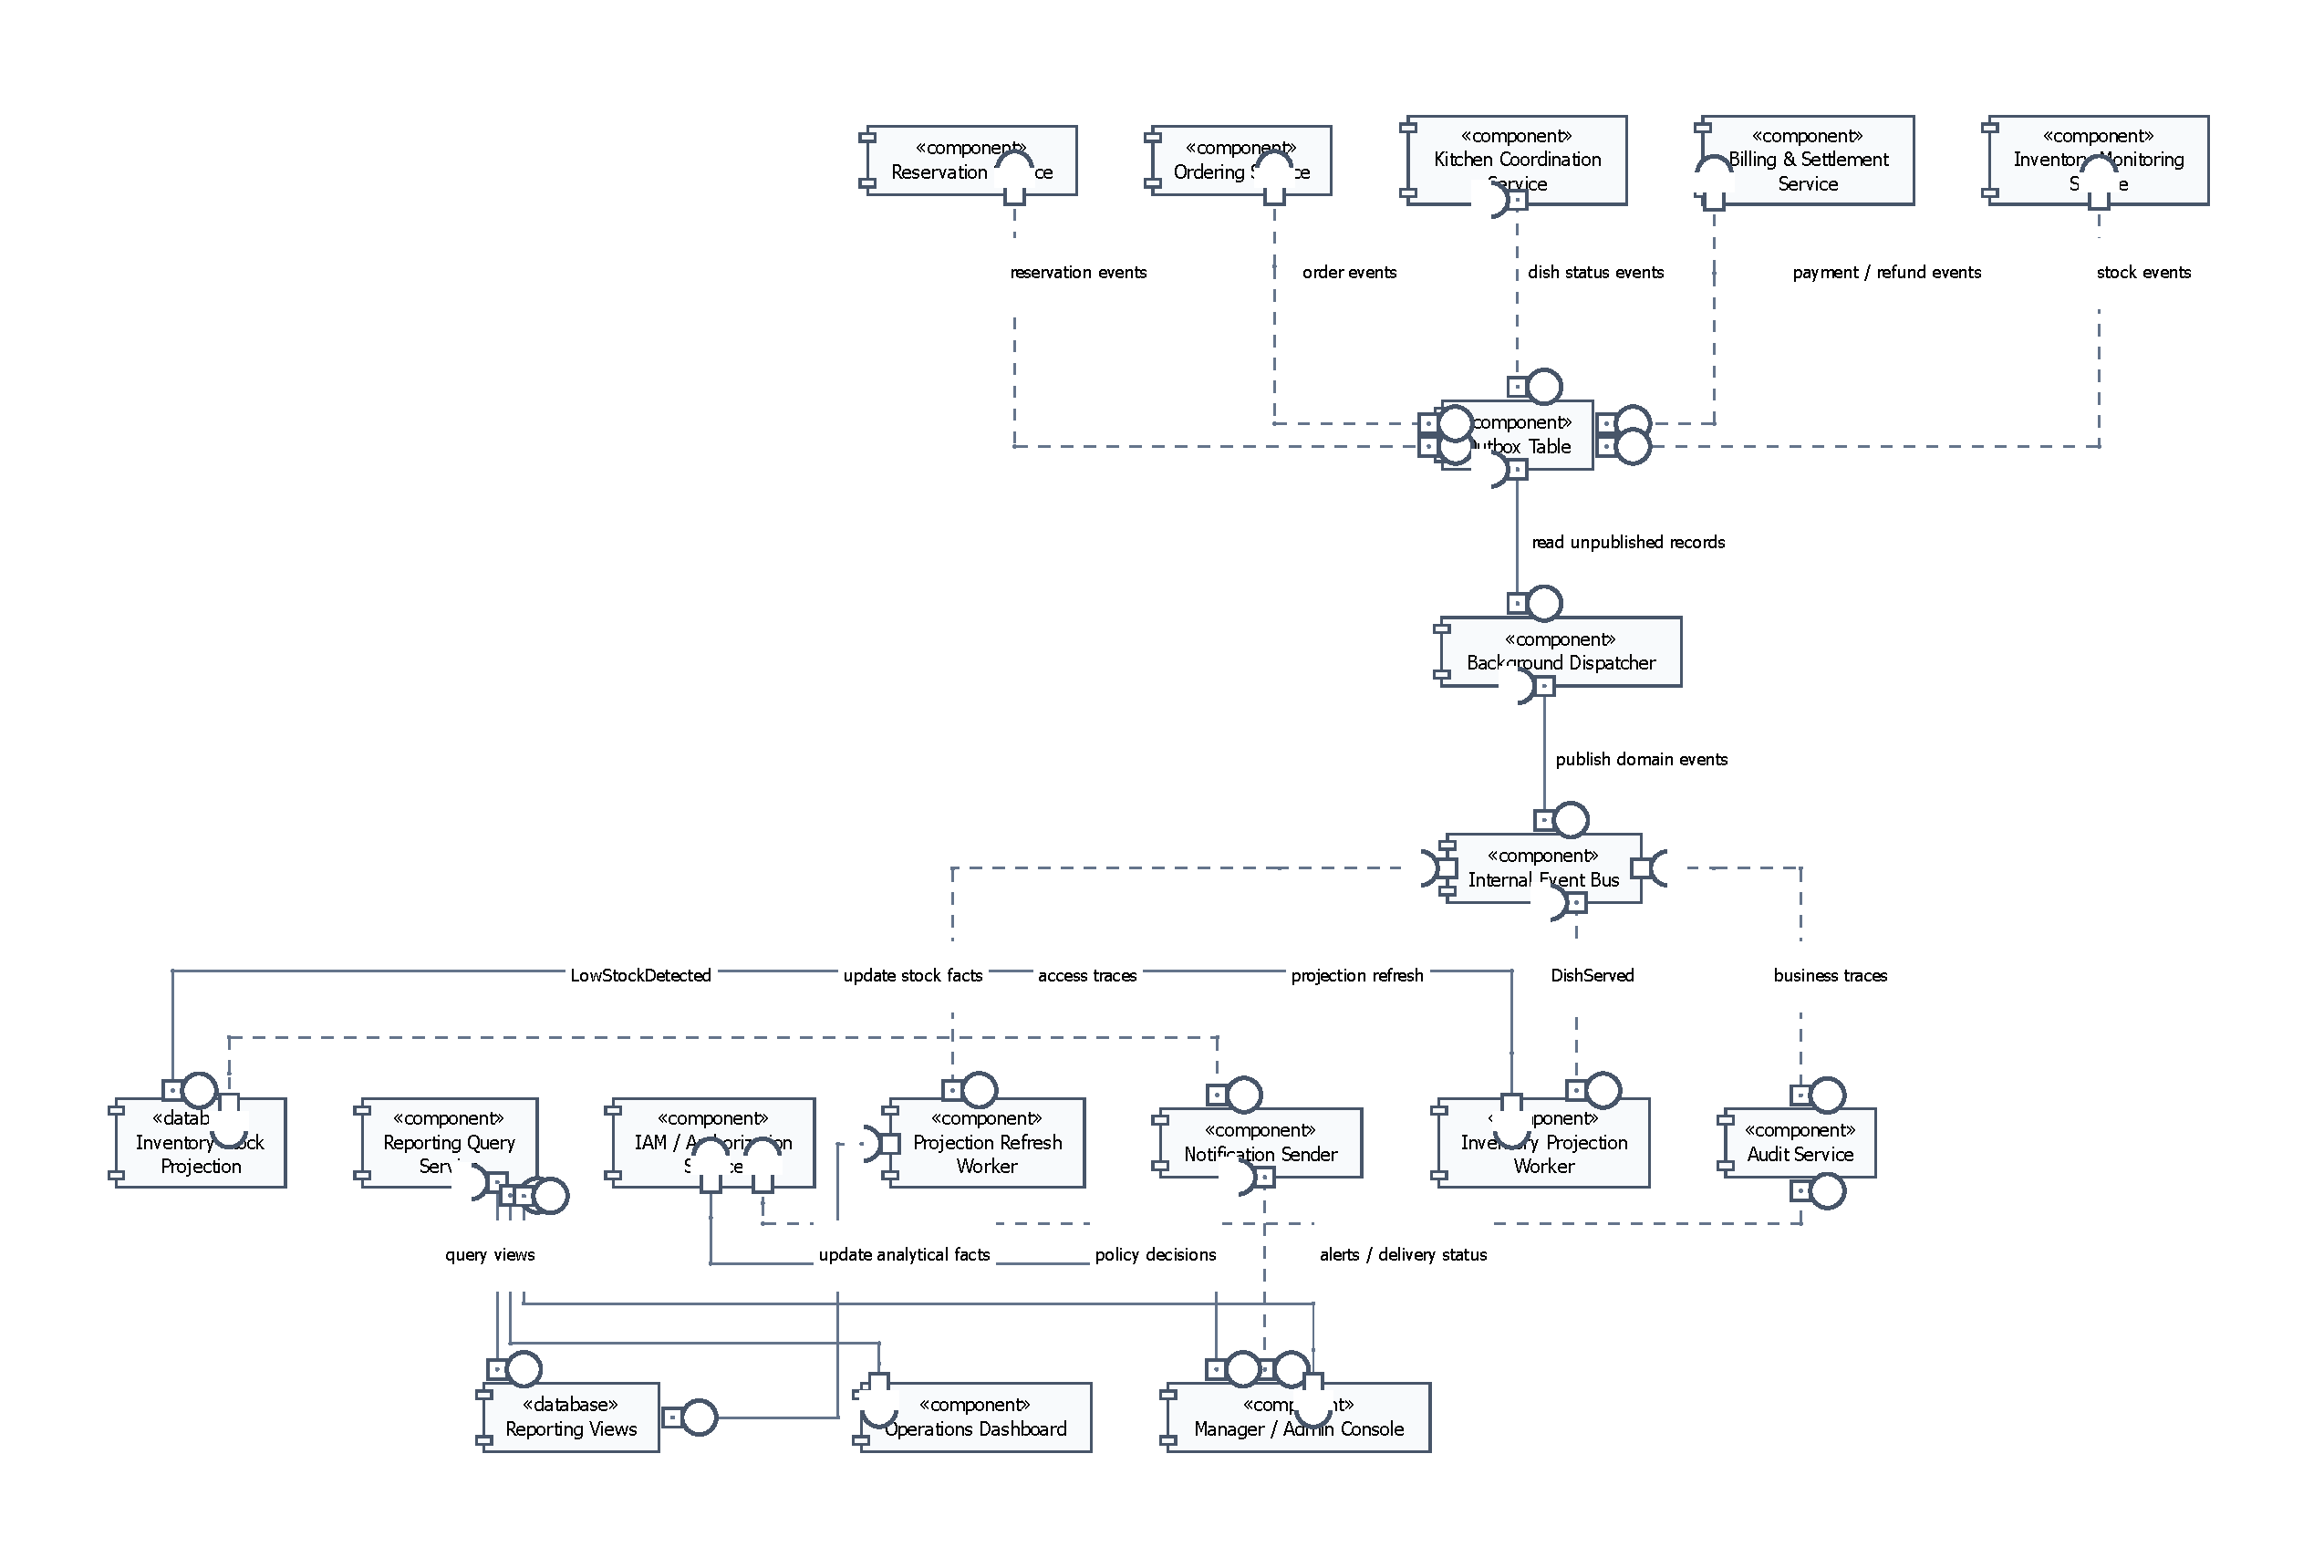
\includegraphics[width=0.97\linewidth,height=0.84\textheight,keepaspectratio]{25_component_diagram_supporting_async_and_governance.pdf}
}{
  \IfFileExists{25_component_diagram_supporting_async_and_governance.png}{
    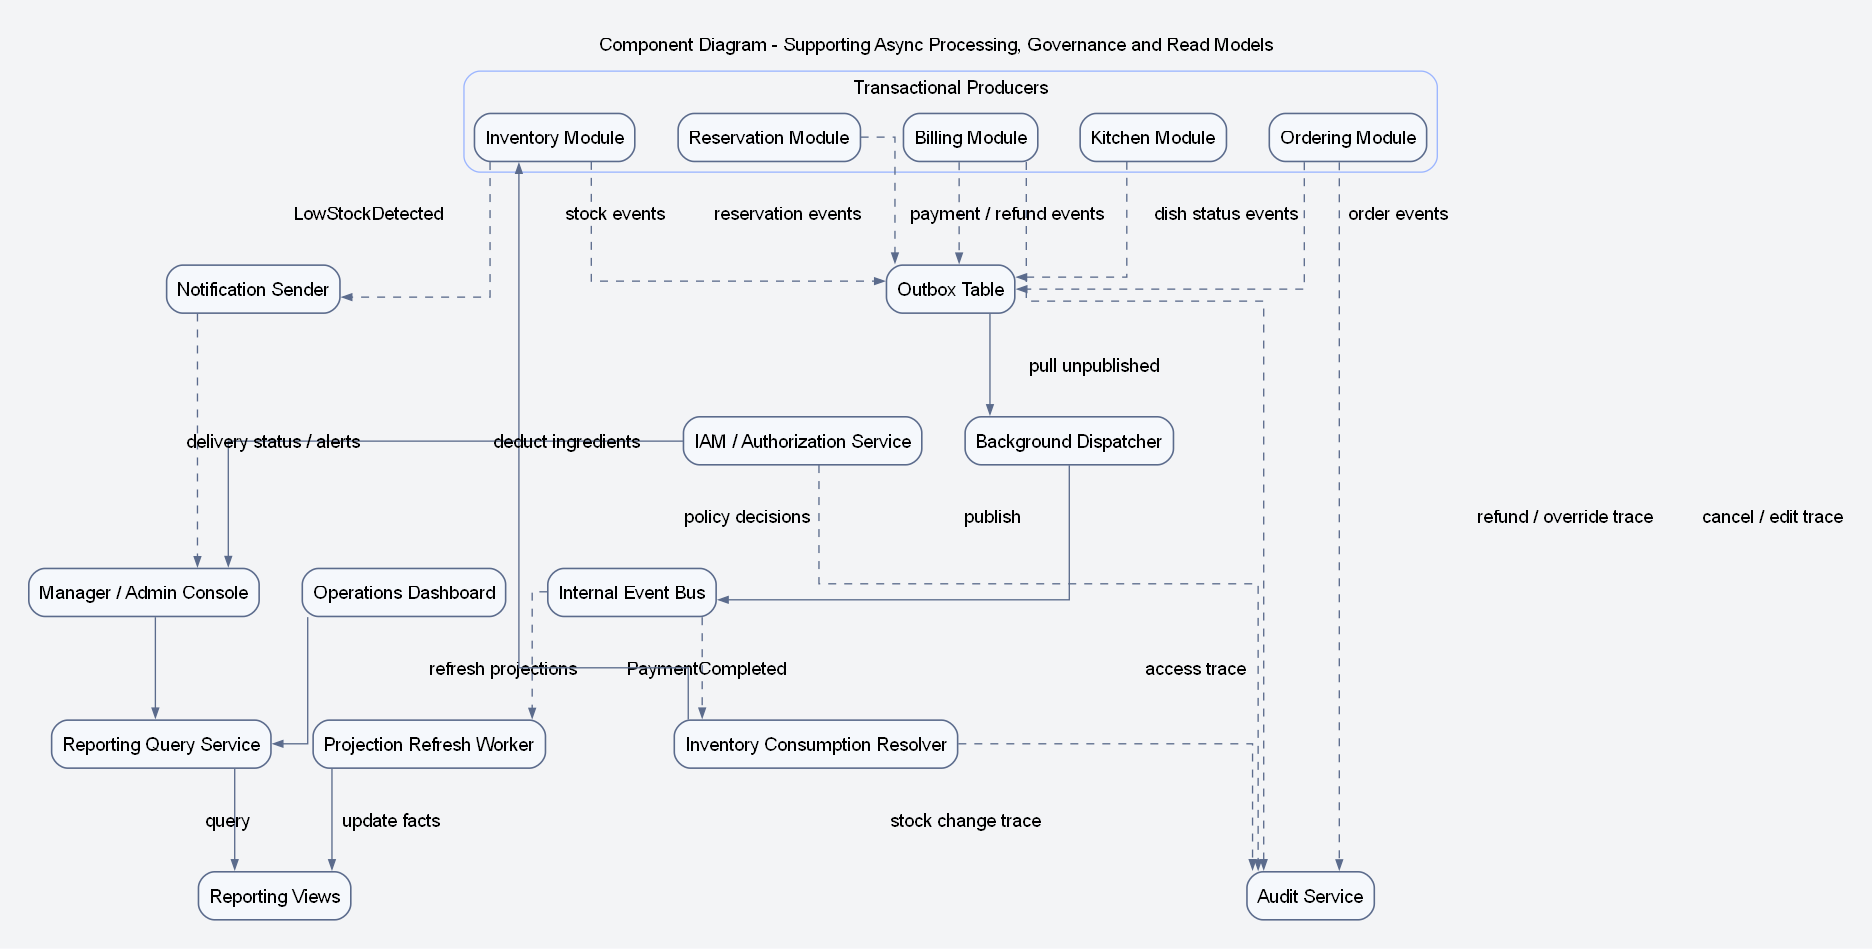
\includegraphics[width=0.97\linewidth,height=0.84\textheight,keepaspectratio]{25_component_diagram_supporting_async_and_governance.png}
  }{
    \fbox{\parbox{0.82\linewidth}{Thiếu file \textsf{25\_component\_diagram\_supporting\_async\_and\_governance.(pdf/png)}.}}
  }
}
\caption{Sơ đồ thành phần cho xử lý nền, quản trị và mô hình đọc}
\label{fig:irms-component-supporting-async}
\end{figure}


Hình~\ref{fig:irms-component-supporting-async} mô tả kiến trúc event-driven sau khi các giao dịch lõi đã được xác lập. Đây là Component Diagram của C\&C View, không phải Class Diagram: các phần tử trong hình là service, outbox, RabbitMQ và bộ xử lý sự kiện nền đang tham gia vào tương tác runtime. Tại đây, IRMS tập trung vào việc hiện thực hóa nguyên tắc \textbf{Nhất quán cuối cùng (Eventual Consistency)} và \textbf{Tách biệt trách nhiệm truy vấn (CQRS - Command Query Responsibility Segregation)} ở mức độ thực dụng.

Cấu trúc phối hợp giữa các thành phần hỗ trợ được tổ chức như sau:

\begin{enumerate}
    \item \textbf{Cơ chế phát và chuyển tiếp sự kiện:} Các service giao dịch ghi sự kiện vào \textsf{outbox\_events}. Sau đó \textsf{RabbitMqOutboxRelay} đọc bản ghi chưa phát, dùng \textsf{RabbitMqEventPublisher} đẩy sự kiện sang \textsf{RabbitMQ}. Cấu trúc này khớp với \texttt{TransactionalOutboxPublisher}, \texttt{RabbitMqOutboxRelay} và cấu hình \texttt{spring.rabbitmq.*} trong backend.

    \item \textbf{Cơ chế diễn dịch sự kiện (Event Projection):} Các sự kiện sau khi đi qua \textsf{RabbitMQ} được tiêu thụ bởi các bộ xử lý sự kiện như \textsf{ReportingProjectionConsumer} và \textsf{InventoryStockChangedConsumer}. Các thành phần này chuyển dữ liệu từ dạng giao dịch sang mô hình đọc hoặc projection phục vụ báo cáo và tồn kho, giúp yêu cầu từ màn hình quản lý không tranh chấp trực tiếp với luồng gọi món.
    
    \item \textbf{Quản trị và Tuân thủ (Governance \& Compliance):} 
    \begin{itemize}
        \item \textsf{AuditRecordingRequestedConsumer}: Độc lập với logic nghiệp vụ, chỉ tiêu thụ event để ghi audit log (lưu vết: ai, làm gì, khi nào, ngữ
        \item \textbf{IAM / Authorization Service:} Cung cấp các chính sách bảo vệ tài nguyên (Policy-based Access Control), đảm bảo các thao tác quản trị nhạy cảm như hoàn tiền hoặc điều chỉnh tồn kho luôn được kiểm soát chặt chẽ.
    \end{itemize}

    \item \textbf{Tích hợp thông báo và liên lạc (Notification Hub):} \textsf{NotificationRequestedConsumer} tiếp nhận sự kiện từ \textsf{RabbitMQ}; sau đó \textsf{NotificationService} ghi nhận thông báo qua các adapter kênh trong thiết kế:
    \begin{itemize}
        \item \textsf{EmailNotificationChannelAdapter}, \textsf{SmsNotificationChannelAdapter};
        \item \textsf{InAppNotificationChannelAdapter}, \textsf{PrintNotificationChannelAdapter}.
    \end{itemize}
    Thiết kế hiện tại chưa thể hiện nhà cung cấp SMS/Email bên ngoài hay máy in vật lý, nên phần này chỉ được hiểu là biên adapter nội bộ.
\end{enumerate}

\paragraph{Cơ sở thiết kế xử lý nền:}
\begin{itemize}
  \item \textbf{Tối ưu hóa tài nguyên ghi (Write Optimization):} Đẩy các tác vụ phụ (tổng hợp báo cáo, gửi thông báo) sang xử lý nền giúp giảm tải DB giao dịch chính, tối ưu tốc độ phản hồi cho các nghiệp vụ lõi (chốt đơn, thanh toán).
  \item \textbf{Khả năng quan sát (Observability):} Tách biệt các event consumer giúp dễ dàng monitor trạng thái và độ trễ của từng tác vụ (cập nhật projection, audit log, notification) thông qua log và các bảng \textsf{outbox\_events}, \textsf{processed\_events}.
\end{itemize}

\subsection{Góc nhìn triển khai}\label{sec:deployment-view}
\subsubsection{Tổng quan phân bổ hệ thống}

Ở góc nhìn triển khai, hệ thống được ánh xạ lên hạ tầng vật lý và hạ tầng thực thi nhằm làm rõ cách các thành phần phần mềm được phân bổ trên các nút triển khai (deployment nodes), cách các nút này giao tiếp với nhau và cách hệ thống đáp ứng các yêu cầu phi chức năng như độ trễ, khả năng mở rộng và độ tin cậy. Mô hình này nhất quán với \adrref{ADR-0008}{adr:0008-single-postgresql} về một PostgreSQL vật lý duy nhất và \adrref{ADR-0014}{adr:0014-docker-compose} về Docker Compose cho runtime cục bộ.

Hệ thống được tổ chức thành bốn tầng chính như sau:

\begin{enumerate}

  \item \textbf{Tầng thiết bị đầu cuối (Client Layer)}
  \begin{itemize}
    \item Máy tính bảng dành cho nhân viên phục vụ, hỗ trợ thao tác đặt bàn và gọi món theo thời gian thực.
    \item Thiết bị lễ tân hoặc ki-ốt tiếp nhận khách, phục vụ việc đăng ký và phân bổ chỗ ngồi.
    \item Màn hình bếp tại từng trạm chế biến, hiển thị danh sách món cần chuẩn bị với yêu cầu cập nhật gần thời gian thực.
    \item Máy thu ngân, thực hiện các giao dịch thanh toán với yêu cầu độ trễ thấp và tính nhất quán cao.
    \item Trình duyệt của quản lý, phục vụ truy vấn báo cáo và giám sát hoạt động hệ thống.
  \end{itemize}

  Các thiết bị này hoạt động như các client gửi yêu cầu đồng bộ (synchronous request) tới hệ thống thông qua giao thức HTTP/HTTPS. Đặc điểm chung của tầng này là phụ thuộc vào mạng và yêu cầu độ trễ thấp đối với các thao tác nghiệp vụ chính.

  \item \textbf{Tầng cổng vào và phân phối (Gateway \& Delivery Layer)}
  \begin{itemize}
    \item Bộ đảo ngược lưu lượng hoặc \textbf{API Gateway}, đóng vai trò điểm truy cập duy nhất của hệ thống.
    \item Máy chủ phân phối giao diện tĩnh hoặc giao diện phía máy chủ, chịu trách nhiệm phục vụ nội dung frontend.
  \end{itemize}

  Tầng này chịu trách nhiệm:
  \begin{itemize}
    \item Điều phối yêu cầu từ client tới các service tương ứng.
    \item Thực hiện các kiểm tra kỹ thuật chung như xác thực, phân quyền và ghi nhận nhật ký truy cập.
    \item Giảm tải cho các service phía sau thông qua việc gom và chuẩn hóa các điểm truy cập.
  \end{itemize}

  Việc sử dụng API Gateway giúp cô lập tầng client với tầng ứng dụng, đồng thời tạo điều kiện thuận lợi cho việc mở rộng và thay đổi cấu trúc backend trong tương lai.

  \item \textbf{Tầng ứng dụng (Application Layer)}
  \begin{itemize}
    \item Khối xử lý phía sau bao gồm các service nghiệp vụ chính:
    \begin{itemize}
      \item Service đặt bàn và quản lý chỗ ngồi.
      \item Service gọi món và thực đơn.
      \item Service điều phối bếp.
      \item Service thanh toán.
      \item Service quản lý tồn kho.
      \item Service báo cáo và quản trị.
      \item Service quản lý truy cập và kiểm toán.
    \end{itemize}

    \item Bộ xử lý nền (Background Worker) thực hiện các tác vụ bất đồng bộ:
    \begin{itemize}
      \item Xử lý sự kiện phát sinh từ hệ thống (event-driven processing).
      \item Thực hiện các tác vụ retry khi xảy ra lỗi tạm thời.
      \item Làm mới các ảnh chụp dữ liệu phục vụ báo cáo (reporting projections).
    \end{itemize}
  \end{itemize}

  Các service trong tầng này có thể được triển khai trên cùng một cụm máy chủ hoặc container, nhưng được tách biệt về mặt logic theo miền nghiệp vụ. Các giao tiếp giữa service có thể bao gồm:
  \begin{itemize}
    \item Giao tiếp đồng bộ (REST API) cho các thao tác nghiệp vụ chính.
    \item Giao tiếp bất đồng bộ (message queue) cho các tác vụ nền.
  \end{itemize}

  \item \textbf{Tầng dữ liệu (Data Layer)}
  \begin{itemize}
    \item Cơ sở dữ liệu giao dịch, lưu trữ dữ liệu vận hành chính như đơn hàng, thanh toán, tồn kho và người dùng.
    \item Mô hình đọc và khung nhìn báo cáo, được tối ưu cho truy vấn và phân tích dữ liệu.
    \item Các bảng \textsf{outbox\_events}, \textsf{processed\_events} và mô hình đọc báo cáo phục vụ xử lý nền và truy vấn quản trị.
    \item Hạ tầng \textsf{RabbitMQ} phục vụ hàng đợi sự kiện giữa các service.
  \end{itemize}

  Tầng dữ liệu được thiết kế tách biệt với tầng ứng dụng nhằm đảm bảo tính toàn vẹn dữ liệu, đồng thời hỗ trợ mở rộng theo nhu cầu đọc/ghi. Các thành phần như mô hình đọc và hệ thống logging thường được cập nhật thông qua luồng xử lý bất đồng bộ để giảm tải cho hệ thống giao dịch chính.

\end{enumerate}

\subsubsection{Cơ sở thiết kế triển khai}
\begin{itemize}
  \item \textbf{Tối ưu mạng nội bộ:} Thiết bị gọi món và bếp ưu tiên kết nối mạng LAN để giảm latency và đảm bảo vận hành liên tục khi kết nối WAN (Internet) không ổn định.
  \item \textbf{Độ sẵn sàng cao (High Availability):} Các module Billing và Ordering yêu cầu HA cao nhất. Cần ưu tiên giám sát, backup và khả năng scale vì ảnh hưởng trực tiếp đến doanh thu.
  \item \textbf{Tách biệt OLTP và OLAP:} Tách khối báo cáo khỏi tuyến giao dịch để các truy vấn phân tích (nặng) không gây nghẽn luồng xử lý gọi món và thanh toán (thời gian thực).
  \item \textbf{Bảo mật dữ liệu:} Áp dụng chính sách phân quyền và sao lưu riêng biệt cho dữ liệu thanh toán và audit log; đây là nhóm dữ liệu nhạy cảm, yêu cầu bảo vệ cao nhất.
  \item \textbf{Cô lập tài nguyên (Resource Isolation):} Tách bộ xử lý nền (Background Worker) giúp các tác vụ phụ như in biên lai điện tử hay gửi thông báo không tranh chấp tài nguyên với các thao tác tại quầy.
\end{itemize}



\begin{figure}[H]
\centering
\IfFileExists{15_deployment_diagram_physical_deployment_overview.pdf}{
  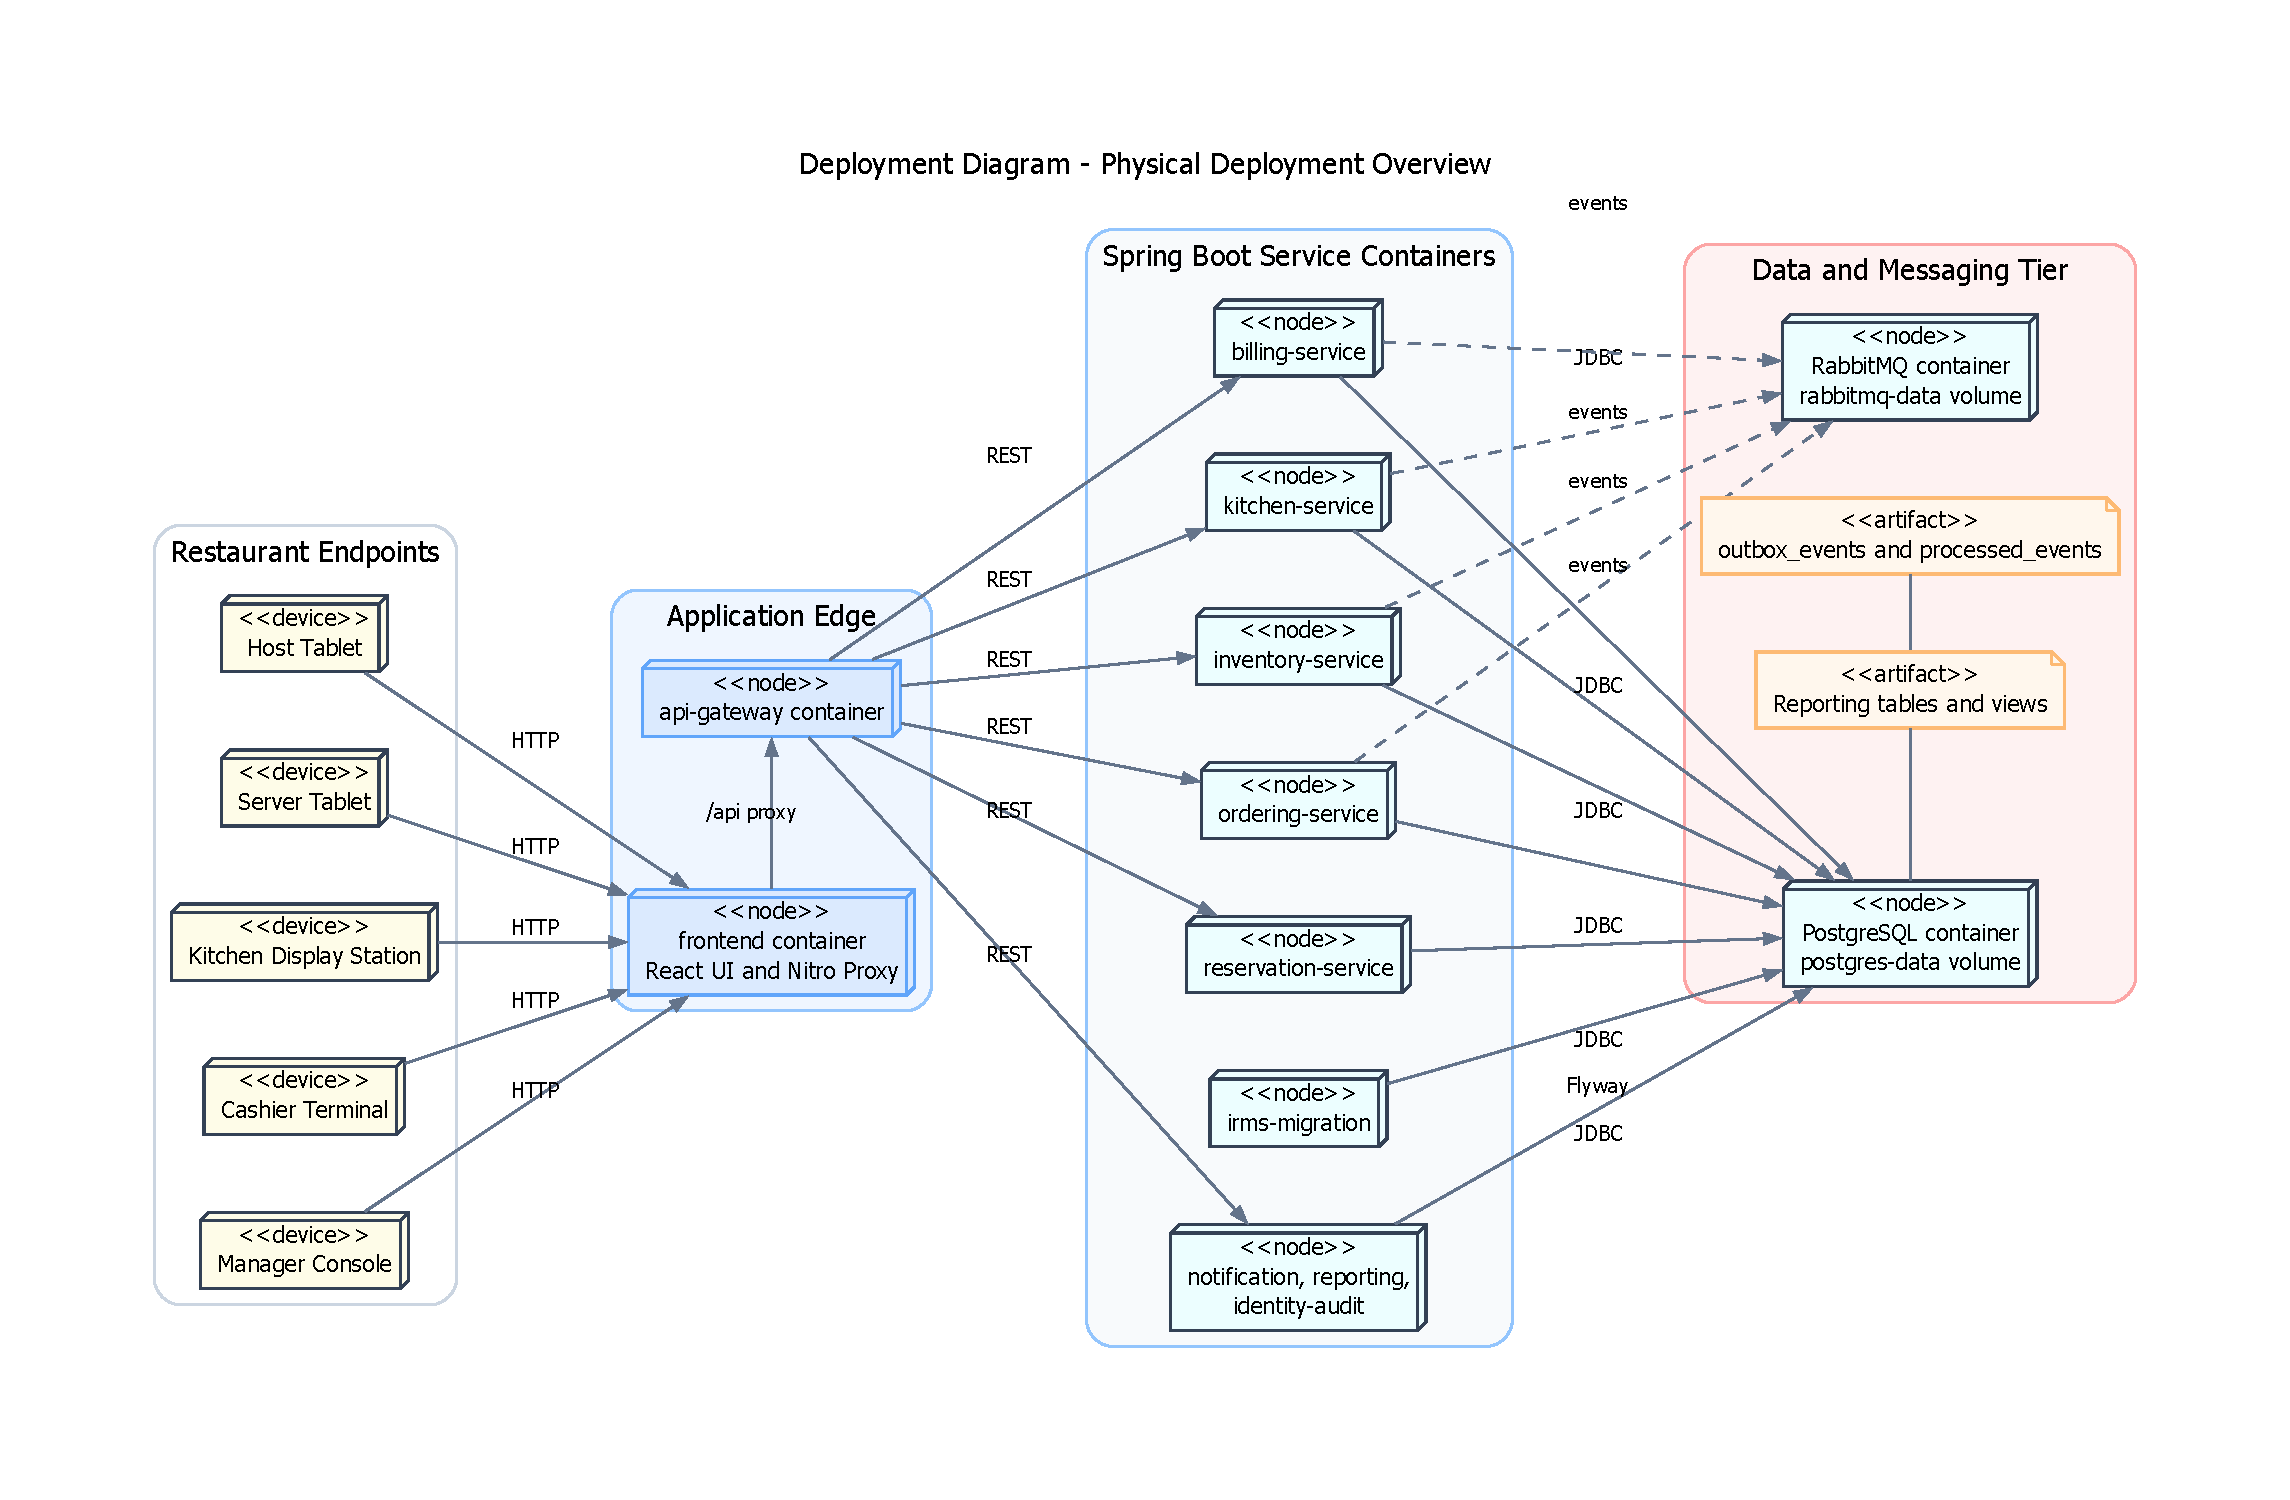
\includegraphics[width=0.97\linewidth,height=0.84\textheight,keepaspectratio]{15_deployment_diagram_physical_deployment_overview.pdf}
}{
  \IfFileExists{15_deployment_diagram_physical_deployment_overview.png}{
    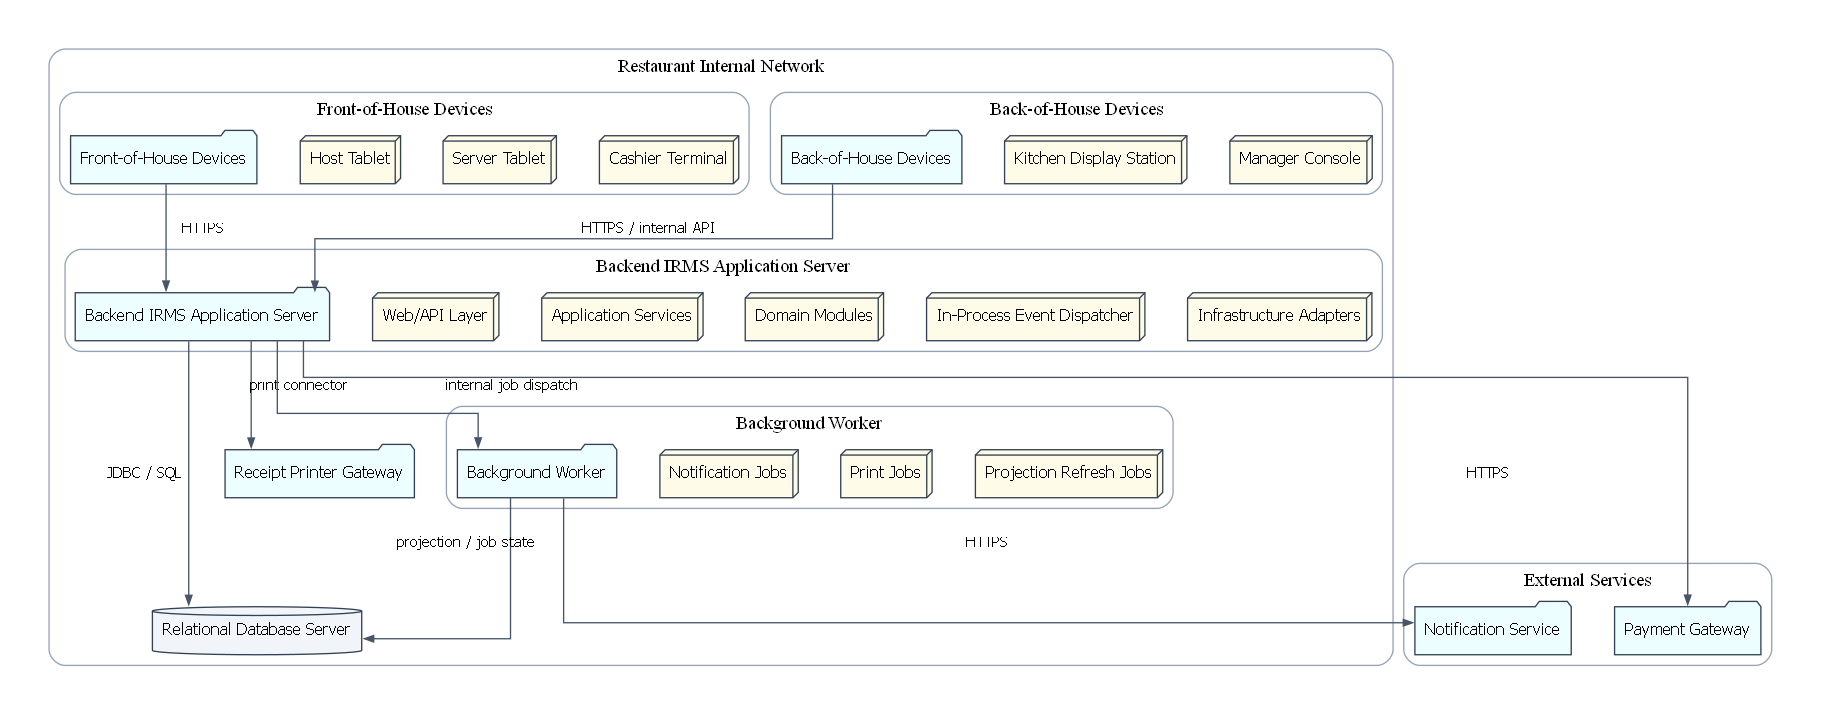
\includegraphics[width=0.97\linewidth,height=0.84\textheight,keepaspectratio]{15_deployment_diagram_physical_deployment_overview.png}
  }{
    \fbox{\parbox{0.82\linewidth}{Thiếu file \textsf{15\_deployment\_diagram\_physical\_deployment\_overview.(pdf/png)}.}}
  }
}
\caption{Sơ đồ triển khai tổng quan về bố trí vật lý của IRMS}
\label{fig:irms-deploy-overall}
\end{figure}

Hình~\ref{fig:irms-deploy-overall} mô tả cách hệ thống được triển khai trong môi trường thực tế của nhà hàng. 

Điểm quan trọng nhất cần rút ra là IRMS được tổ chức theo mô hình \textbf{nhiều điểm chạm vật lý nhưng một lõi điều phối tập trung}. Các thiết bị tại hiện trường --- như máy tính bảng phục vụ, thiết bị lễ tân, màn hình bếp và quầy thu ngân --- được đặt gần người dùng để đảm bảo thao tác nhanh và thuận tiện. Tuy nhiên, toàn bộ trạng thái nghiệp vụ cốt lõi vẫn được duy trì tại khối xử lý trung tâm và hạ tầng dữ liệu, thay vì phân tán xuống các thiết bị.

Cách bố trí này giúp tránh tình trạng mất nhất quán khi mạng dao động hoặc khi nhiều thao tác xảy ra đồng thời tại các điểm khác nhau. Nó cũng phản ánh một nguyên tắc quan trọng: các thiết bị đầu cuối chỉ nên đóng vai trò tương tác, còn quyết định nghiệp vụ bền vững phải được neo tại backend.

Một đặc điểm thiết kế quan trọng khác là sự tách biệt giữa hai tuyến xử lý:

\begin{itemize}
  \item \textbf{Tuyến xử lý trực tuyến (synchronous path)} phục vụ các thao tác yêu cầu phản hồi ngay như gọi món, cập nhật trạng thái bếp và thanh toán.
  \item \textbf{Tuyến xử lý bất đồng bộ (asynchronous path)} xử lý các hệ quả phụ thông qua \textbf{Outbox / hàng đợi} và bộ xử lý nền, bao gồm gửi thông báo, phát hành biên lai và cập nhật dữ liệu báo cáo.
\end{itemize}

Việc phân tách này cho phép hệ thống giữ được thời gian phản hồi ổn định trong giờ cao điểm, khi các thao tác trực tuyến cần được ưu tiên tuyệt đối.

Ngoài ra, sơ đồ cũng làm rõ vai trò của \textsf{PostgreSQL}, \textsf{RabbitMQ}, \textsf{outbox\_events} và các bảng hoặc view báo cáo. Các tác vụ không yêu cầu phản hồi ngay được xử lý tách biệt, trong khi dữ liệu giao dịch chính vẫn được neo trong PostgreSQL để giữ tính nhất quán.

Từ góc độ vận hành, cách bố trí này còn mang lại khả năng \textbf{cô lập lỗi theo thành phần}. Khi bộ xử lý sự kiện nền, hàng đợi hoặc mô hình đọc báo cáo gặp sự cố, tuyến xử lý trực tuyến vẫn có thể tiếp tục hoạt động với mức suy giảm có kiểm soát.

\paragraph{Các thành phần chính}
\begin{itemize}
  \item \textbf{Thiết bị đầu cuối}: máy tính bảng phục vụ, thiết bị lễ tân, màn hình bếp, máy thu ngân và trình duyệt quản lý.
  \item \textbf{Khối cổng vào}: \textsf{frontend container} và \textsf{api-gateway container} tiếp nhận, proxy và định tuyến yêu cầu từ thiết bị.
  \item \textbf{Khối xử lý trung tâm}: các container service Spring Boot thực hiện logic nghiệp vụ chính.
  \item \textbf{Hạ tầng sự kiện}: \textsf{RabbitMQ}, \textsf{outbox\_events} và \textsf{processed\_events} xử lý các tác vụ bất đồng bộ.
  \item \textbf{Hạ tầng dữ liệu}: \textsf{PostgreSQL} lưu dữ liệu giao dịch và mô hình đọc báo cáo.
\end{itemize}

\paragraph{Lý do thiết kế.}
\begin{itemize}
  \item Giữ một lõi xử lý trung tâm giúp đảm bảo tính nhất quán và đơn giản hóa triển khai.
  \item Tách tuyến bất đồng bộ giúp giảm tải cho tuyến trực tuyến.
  \item Phân lớp lưu trữ giúp hệ thống linh hoạt và dễ mở rộng hơn.
\end{itemize}


% =========================

\begin{figure}[H]
\centering
\IfFileExists{16_deployment_diagram_network_zones_and_trust_boundaries.pdf}{
  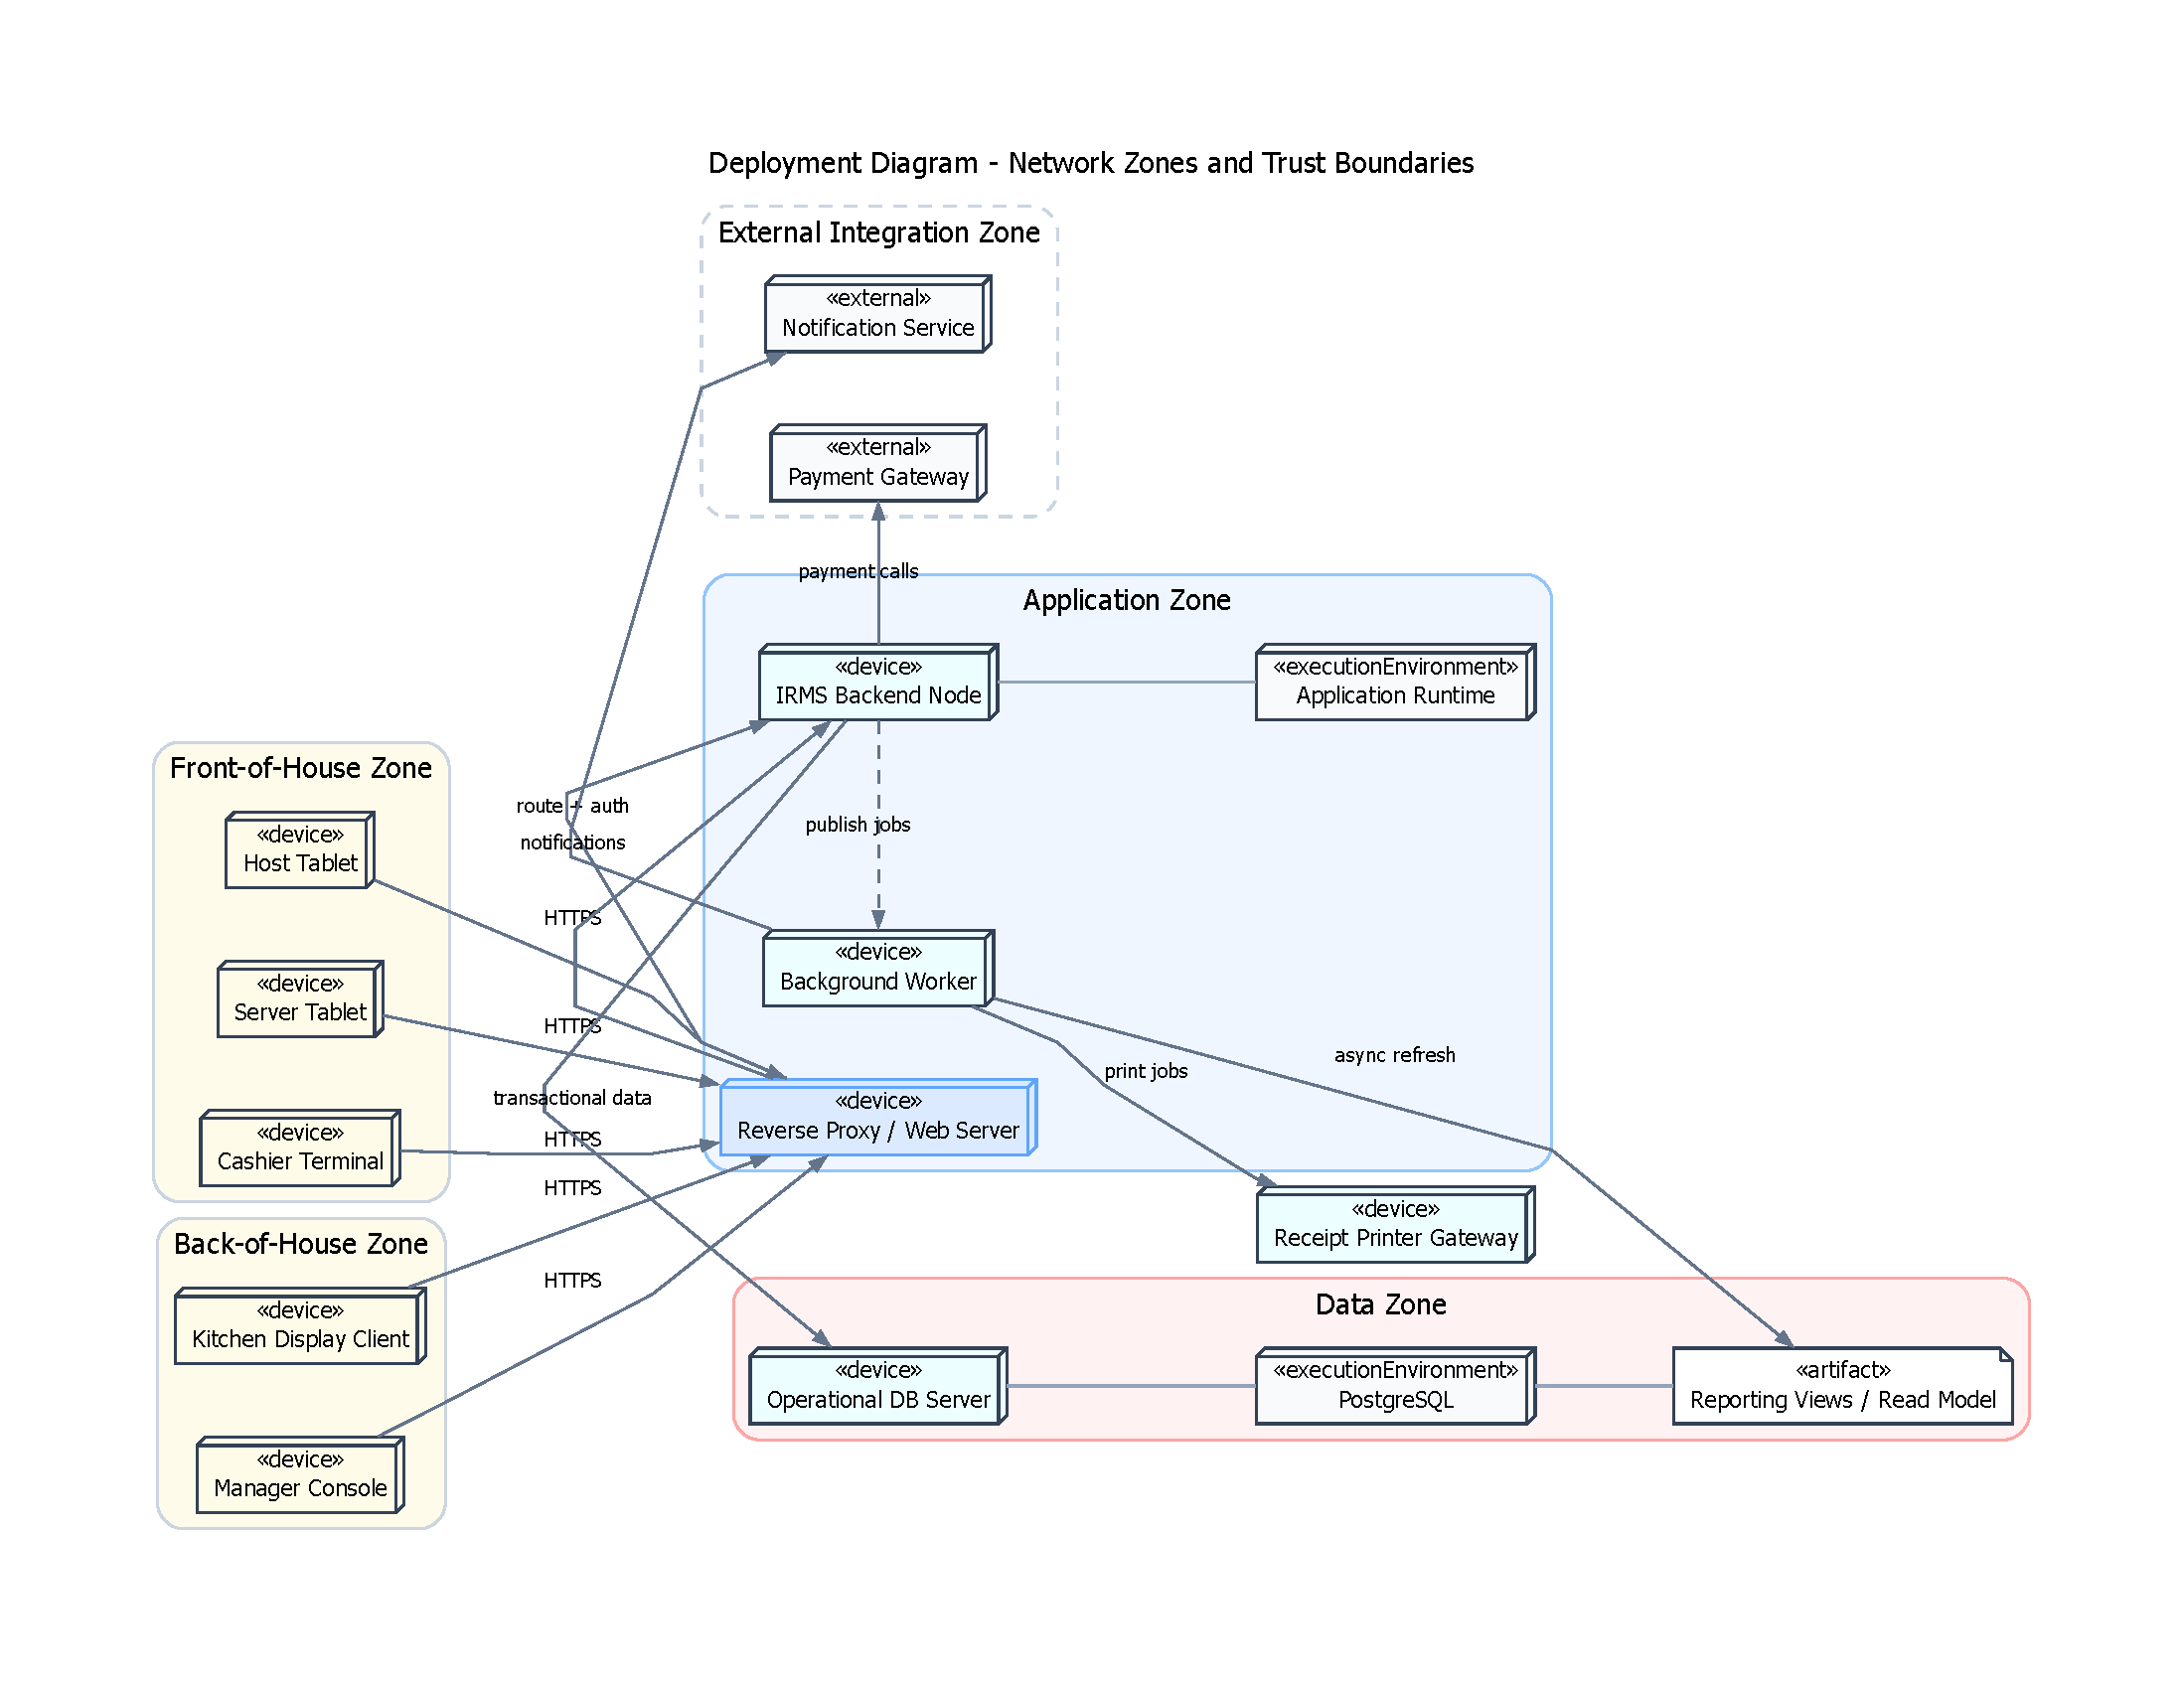
\includegraphics[width=0.97\linewidth,height=0.84\textheight,keepaspectratio]{16_deployment_diagram_network_zones_and_trust_boundaries.pdf}
}{
  \IfFileExists{16_deployment_diagram_network_zones_and_trust_boundaries.png}{
    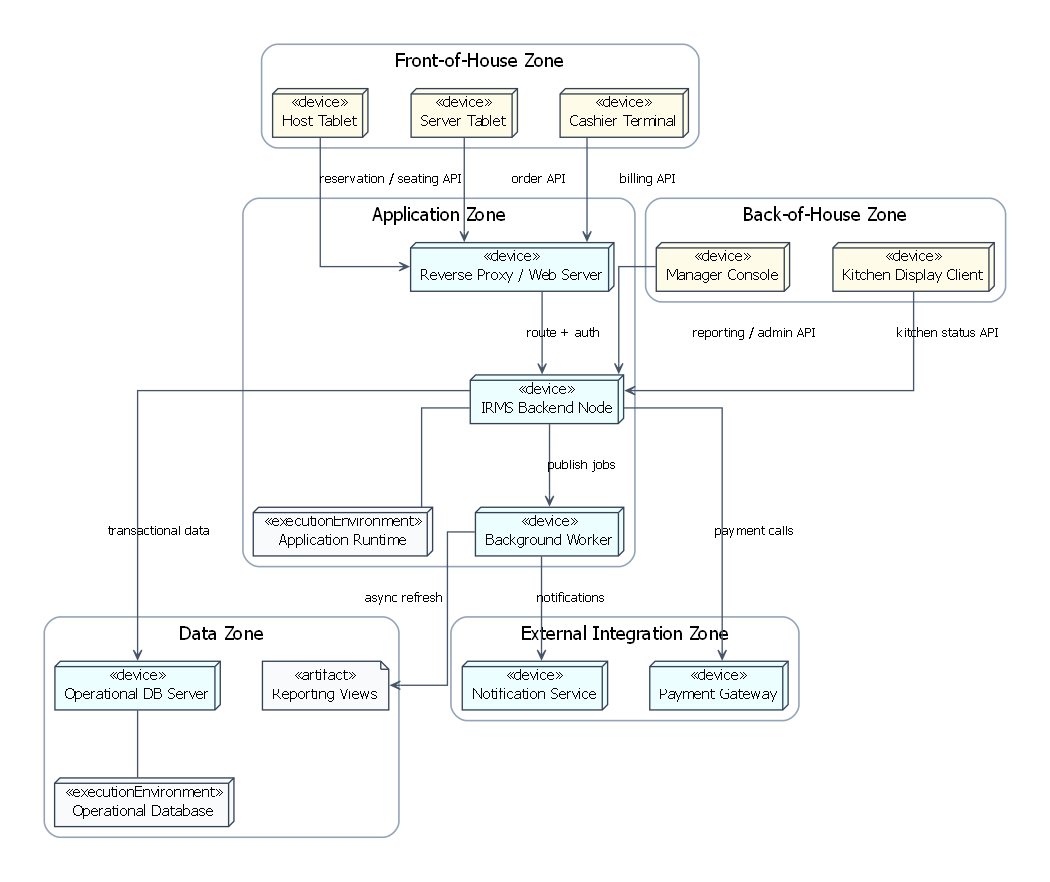
\includegraphics[width=0.97\linewidth,height=0.84\textheight,keepaspectratio]{16_deployment_diagram_network_zones_and_trust_boundaries.png}
  }{
    \fbox{\parbox{0.82\linewidth}{Thiếu file \textsf{16\_deployment\_diagram\_network\_zones\_and\_trust\_boundaries.(pdf/png)}.}}
  }
}
\caption{Sơ đồ triển khai theo vùng mạng và ranh giới tin cậy}
\label{fig:irms-deploy-network}
\end{figure}

Hình~\ref{fig:irms-deploy-network} mở rộng góc nhìn triển khai bằng cách làm rõ \textbf{ranh giới tin cậy} và cách hệ thống được phân chia thành các vùng mạng khác nhau.

Kiến trúc được chia thành các vùng: vùng thiết bị hiện trường, vùng ứng dụng, vùng dữ liệu và vùng hàng đợi sự kiện. Mỗi vùng đại diện cho một mức độ tin cậy và quyền truy cập khác nhau.

Nguyên tắc quan trọng nhất là \textbf{không có thành phần nào được phép vượt qua ranh giới mà không qua kiểm soát}. Các thiết bị đầu cuối chỉ giao tiếp với hệ thống thông qua \textsf{frontend container} và \textsf{api-gateway}. Các service phía sau mới được truy cập \textsf{PostgreSQL} và \textsf{RabbitMQ}.

Việc tách riêng vùng dữ liệu giúp bảo vệ dữ liệu nhạy cảm và giảm nguy cơ truy cập trái phép. Đồng thời, việc đặt \textsf{RabbitMQ} ở vùng riêng giúp cô lập tuyến sự kiện khỏi tuyến yêu cầu trực tuyến.

Sơ đồ này cũng hỗ trợ vận hành thực tế: khi xảy ra sự cố, việc phân vùng giúp nhanh chóng xác định lỗi thuộc lớp nào.

\paragraph{Các vùng chính.}
\begin{itemize}
  \item Vùng thiết bị hiện trường
  \item Vùng ứng dụng
  \item Vùng dữ liệu
  \item Vùng dữ liệu và hàng đợi sự kiện
\end{itemize}

\paragraph{Lý do thiết kế.}
\begin{itemize}
  \item Tăng cường bảo mật thông qua phân tách vùng
  \item Kiểm soát luồng truy cập giữa các thành phần
  \item Hỗ trợ vận hành và xử lý sự cố
\end{itemize}

% =========================

\begin{figure}[H]
\centering
\IfFileExists{17_deployment_diagram_data_and_execution_mapping.pdf}{
  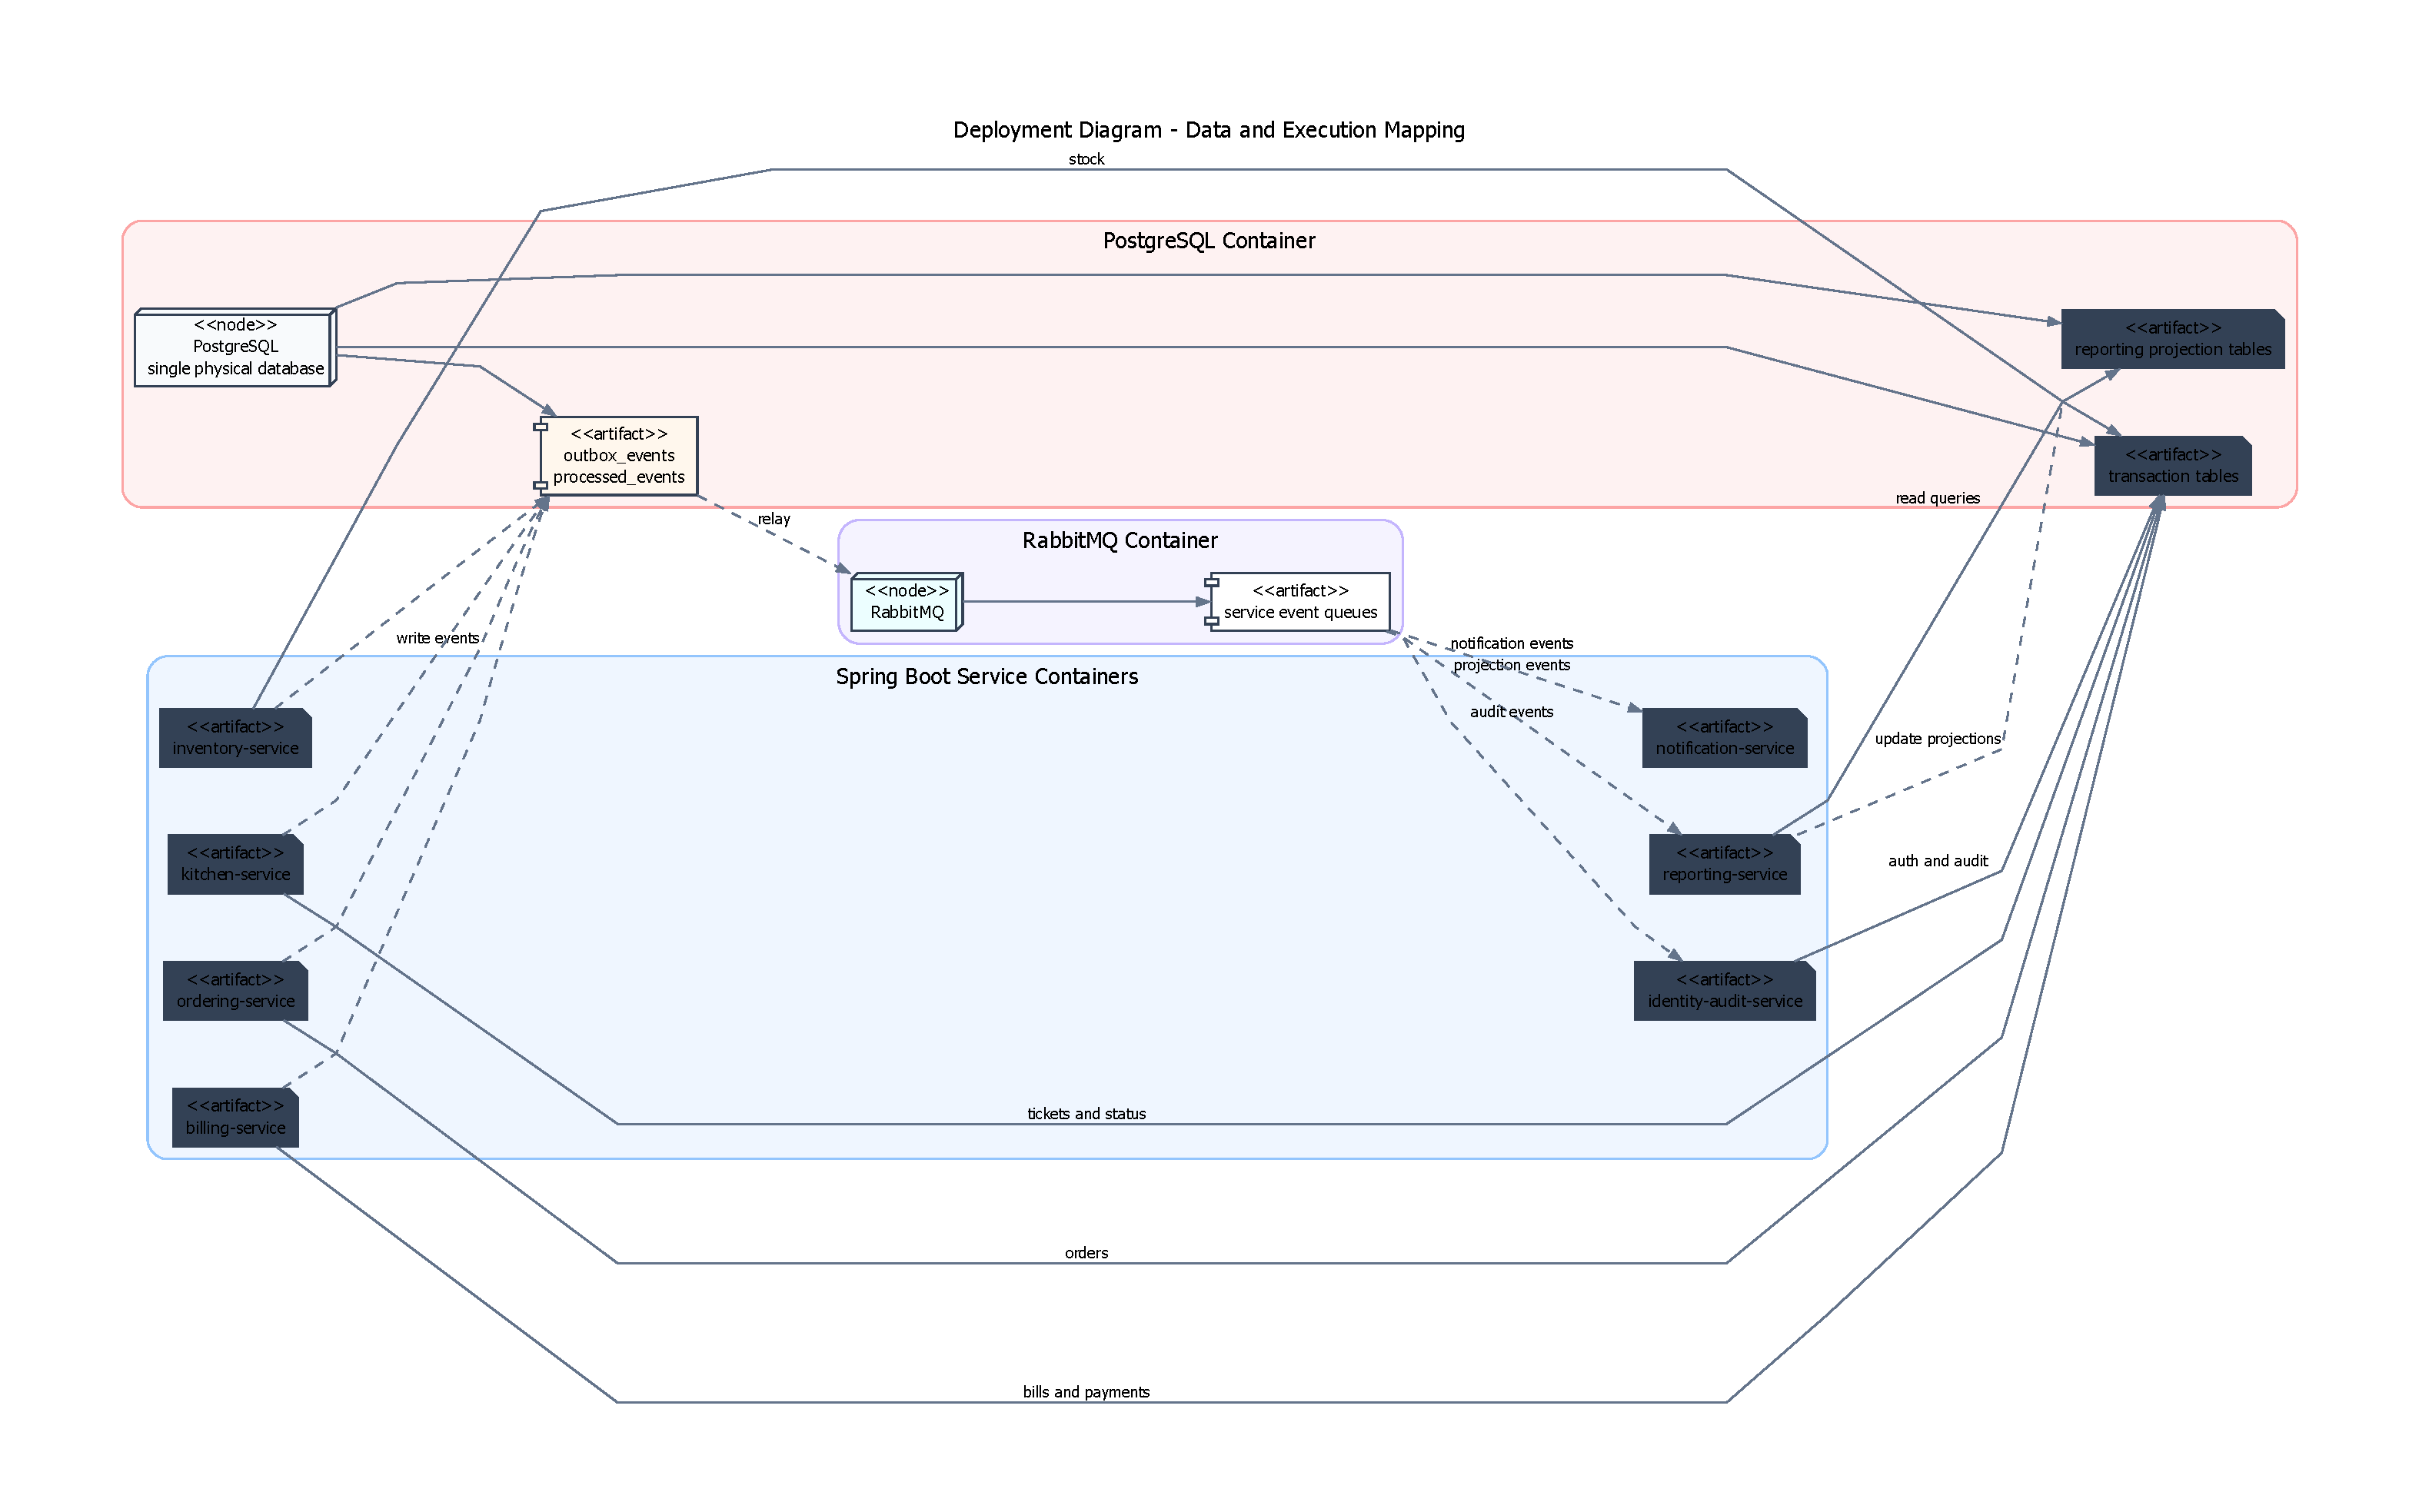
\includegraphics[width=0.97\linewidth,height=0.84\textheight,keepaspectratio]{17_deployment_diagram_data_and_execution_mapping.pdf}
}{
  \IfFileExists{17_deployment_diagram_data_and_execution_mapping.png}{
    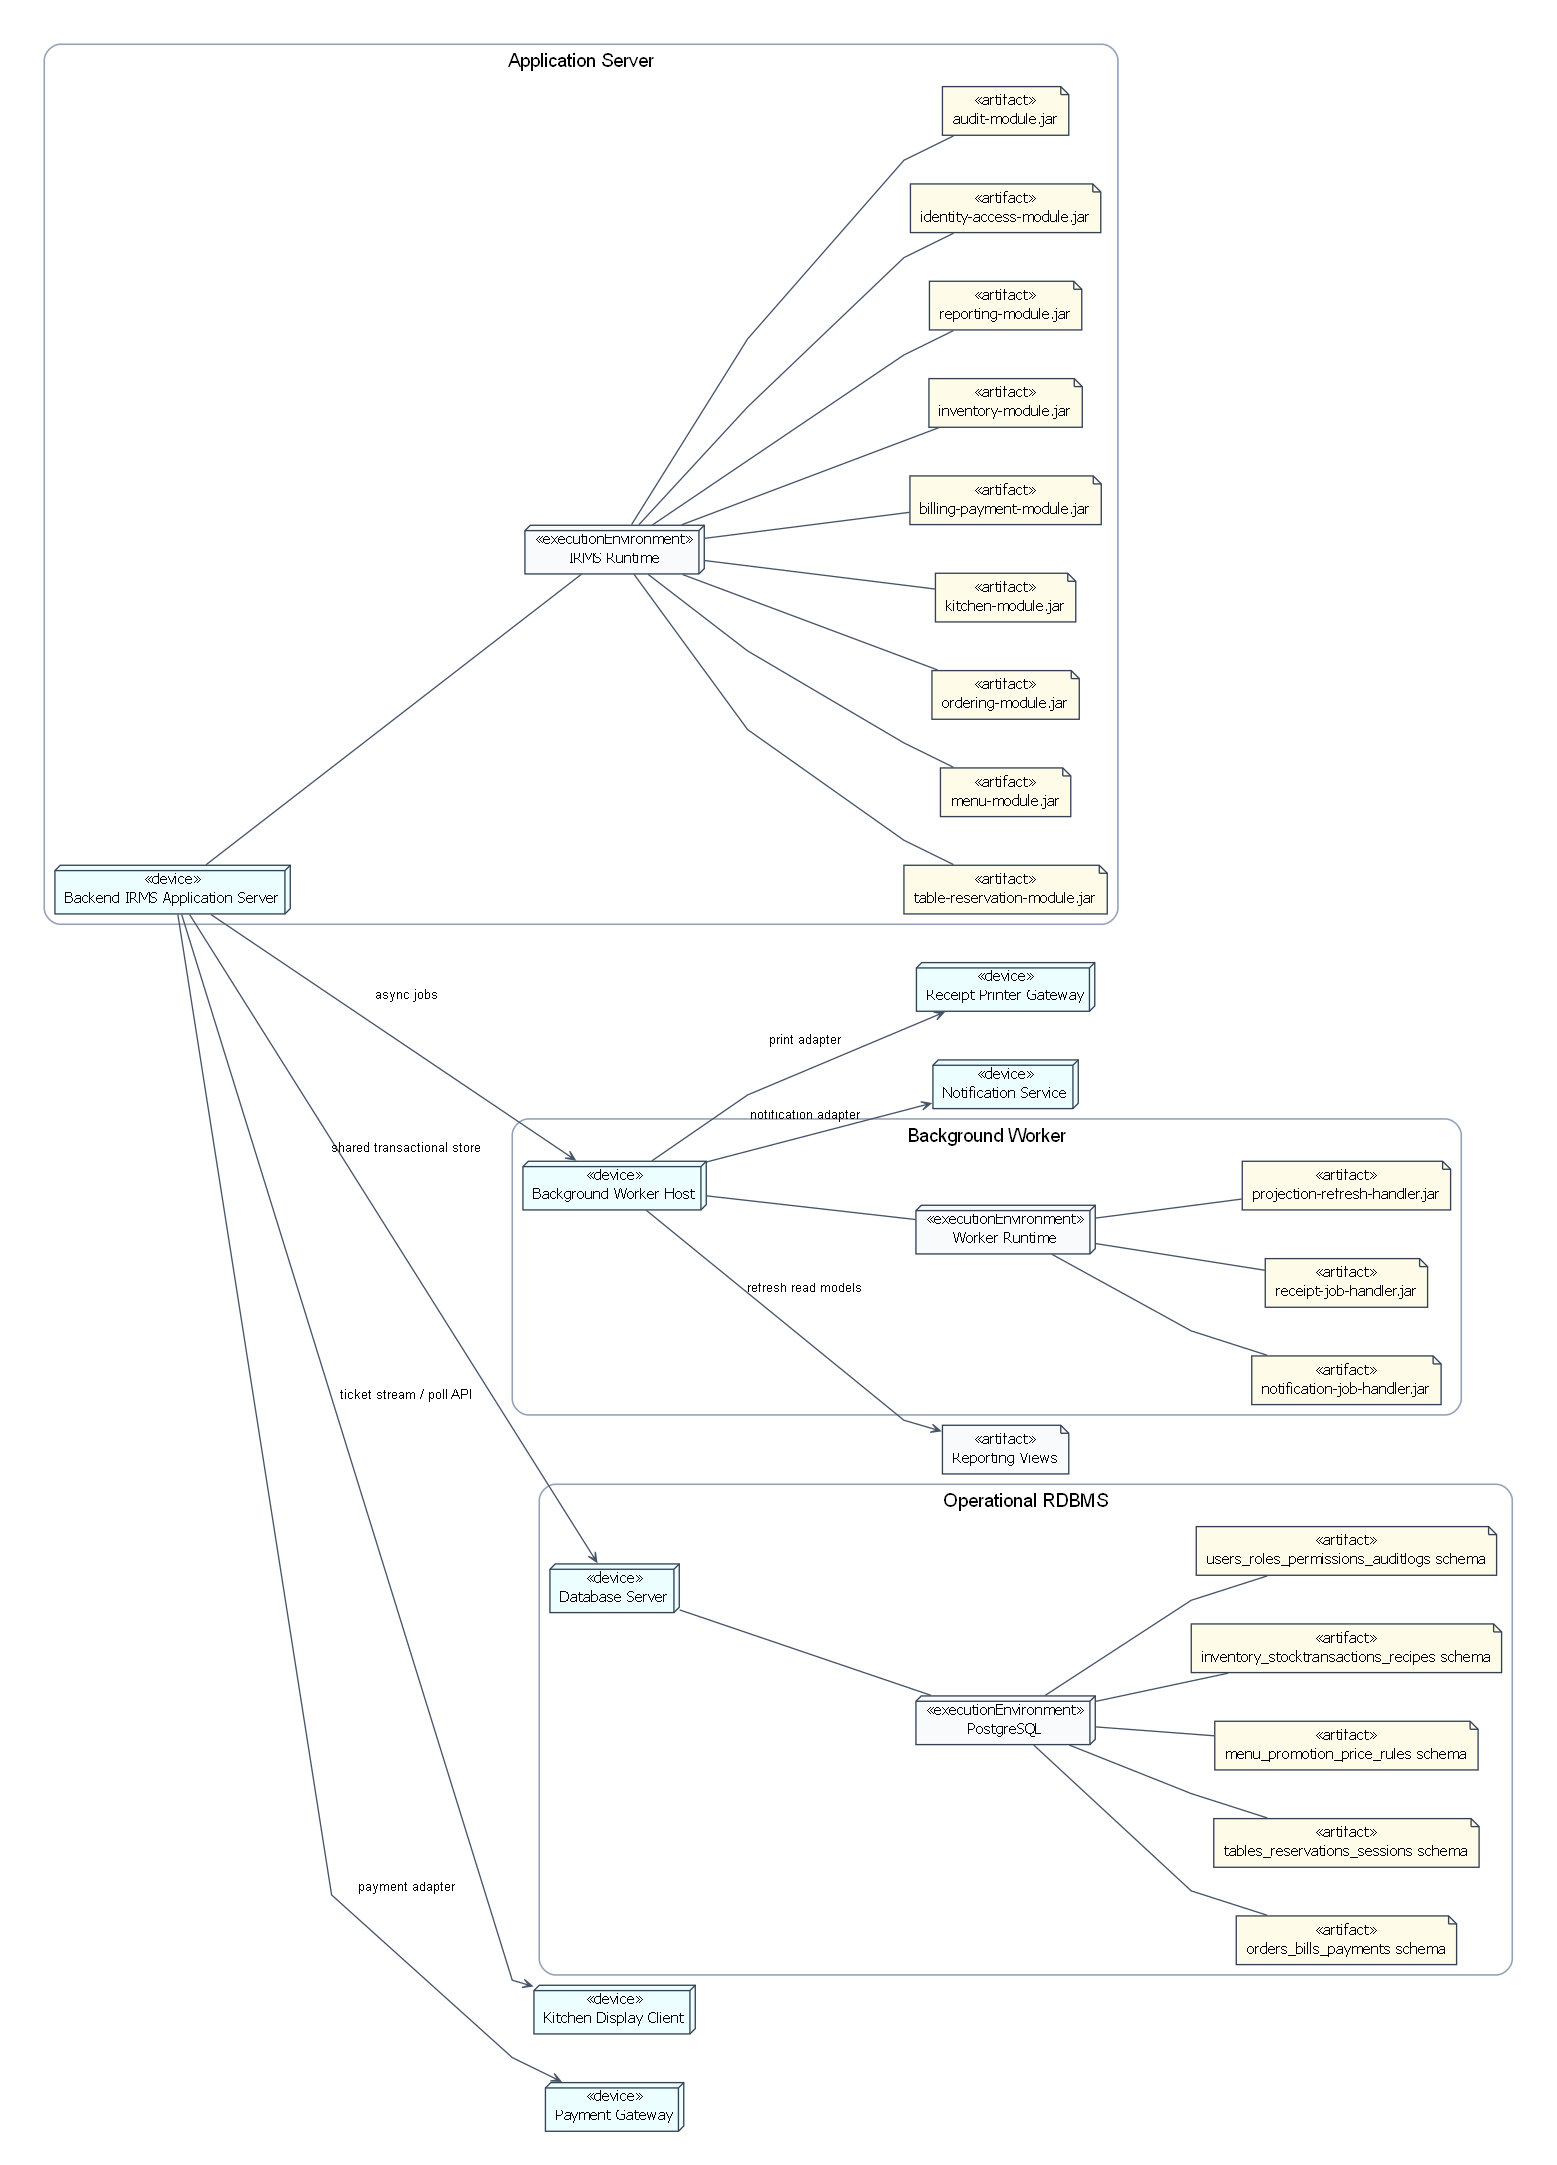
\includegraphics[width=0.97\linewidth,height=0.84\textheight,keepaspectratio]{17_deployment_diagram_data_and_execution_mapping.png}
  }{
    \fbox{\parbox{0.82\linewidth}{Thiếu file \textsf{17\_deployment\_diagram\_data\_and\_execution\_mapping.(pdf/png)}.}}
  }
}
\caption{Sơ đồ triển khai về ánh xạ dữ liệu và thực thi}
\label{fig:irms-deploy-data}
\end{figure}

Hình~\ref{fig:irms-deploy-data} làm rõ cách các service, dữ liệu và luồng thực thi được tổ chức trong hệ thống.

Sơ đồ này thể hiện rõ rằng IRMS theo \textbf{kiến trúc hướng dịch vụ kết hợp điều phối bằng sự kiện}. Các service nghiệp vụ xử lý giao dịch chính thông qua API đồng bộ, trong khi các hệ quả phụ được xử lý thông qua cơ chế bất đồng bộ dựa trên \textbf{Outbox và hàng đợi sự kiện}.

Luồng xử lý có thể chia thành hai phần:

\begin{itemize}
  \item \textbf{Luồng giao dịch chính}: các service ghi dữ liệu vào cơ sở dữ liệu giao dịch.
  \item \textbf{Luồng bất đồng bộ}: các sự kiện được ghi vào Outbox, sau đó được bộ xử lý nền tiêu thụ để cập nhật mô hình đọc, gửi thông báo hoặc xử lý các tác vụ phụ.
\end{itemize}

Cách tổ chức này giúp đảm bảo rằng các giao dịch cốt lõi vẫn rõ ràng và nhất quán, trong khi hệ thống vẫn linh hoạt trong việc xử lý các nhu cầu mở rộng như báo cáo và tích hợp.

Ngoài ra, việc tách mô hình đọc khỏi dữ liệu giao dịch cho phép tối ưu hóa truy vấn mà không ảnh hưởng đến hiệu năng của hệ thống chính.

\paragraph{Các thành phần chính.}
\begin{itemize}
  \item Service nghiệp vụ
  \item Cơ sở dữ liệu giao dịch
  \item Outbox / hàng đợi sự kiện
  \item Bộ xử lý nền
  \item Mô hình đọc
  \item RabbitMQ và các consumer sự kiện
\end{itemize}

\paragraph{Lý do thiết kế.}
\begin{itemize}
  \item Giữ ranh giới service rõ ràng
  \item Tách xử lý bất đồng bộ để giảm phụ thuộc
  \item Tối ưu hóa truy vấn thông qua mô hình đọc
\end{itemize}

Ưu điểm của kiến trúc này là vừa đảm bảo tính rõ ràng của giao dịch, vừa hỗ trợ mở rộng linh hoạt. Đổi lại, hệ thống cần được thiết kế cẩn thận về hợp đồng API, sự kiện và quyền sở hữu dữ liệu để tránh phụ thuộc chéo giữa các service.

\subsubsection{Sơ đồ triển khai cho runtime Docker local và cô lập lỗi}
\begin{figure}[H]
\centering
\IfFileExists{32_deployment_diagram_high_availability_and_failure_isolation.pdf}{
  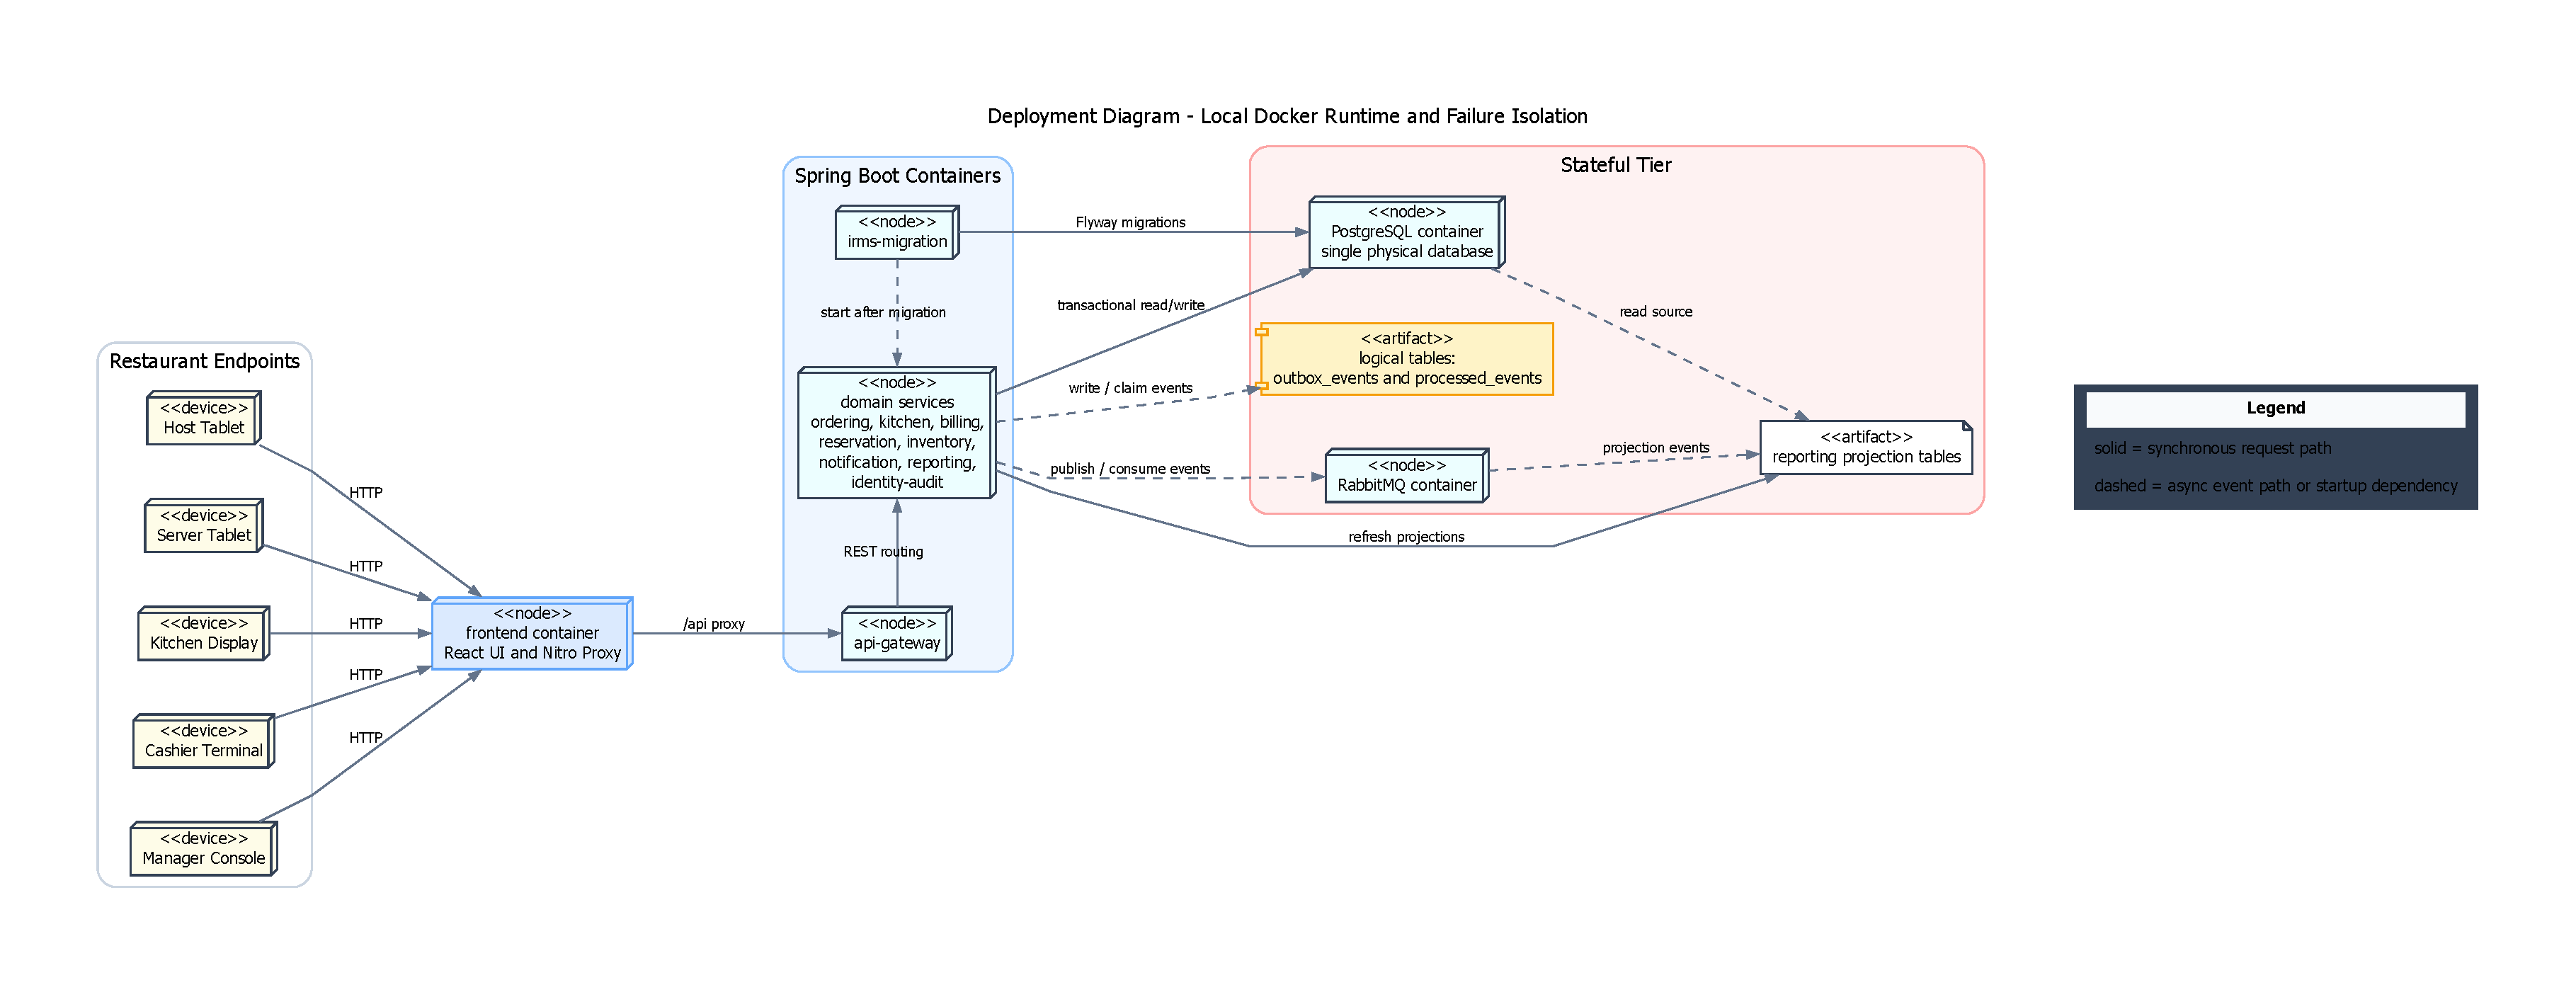
\includegraphics[width=0.97\linewidth,height=0.84\textheight,keepaspectratio]{32_deployment_diagram_high_availability_and_failure_isolation.pdf}
}{
  \IfFileExists{32_deployment_diagram_high_availability_and_failure_isolation.png}{
    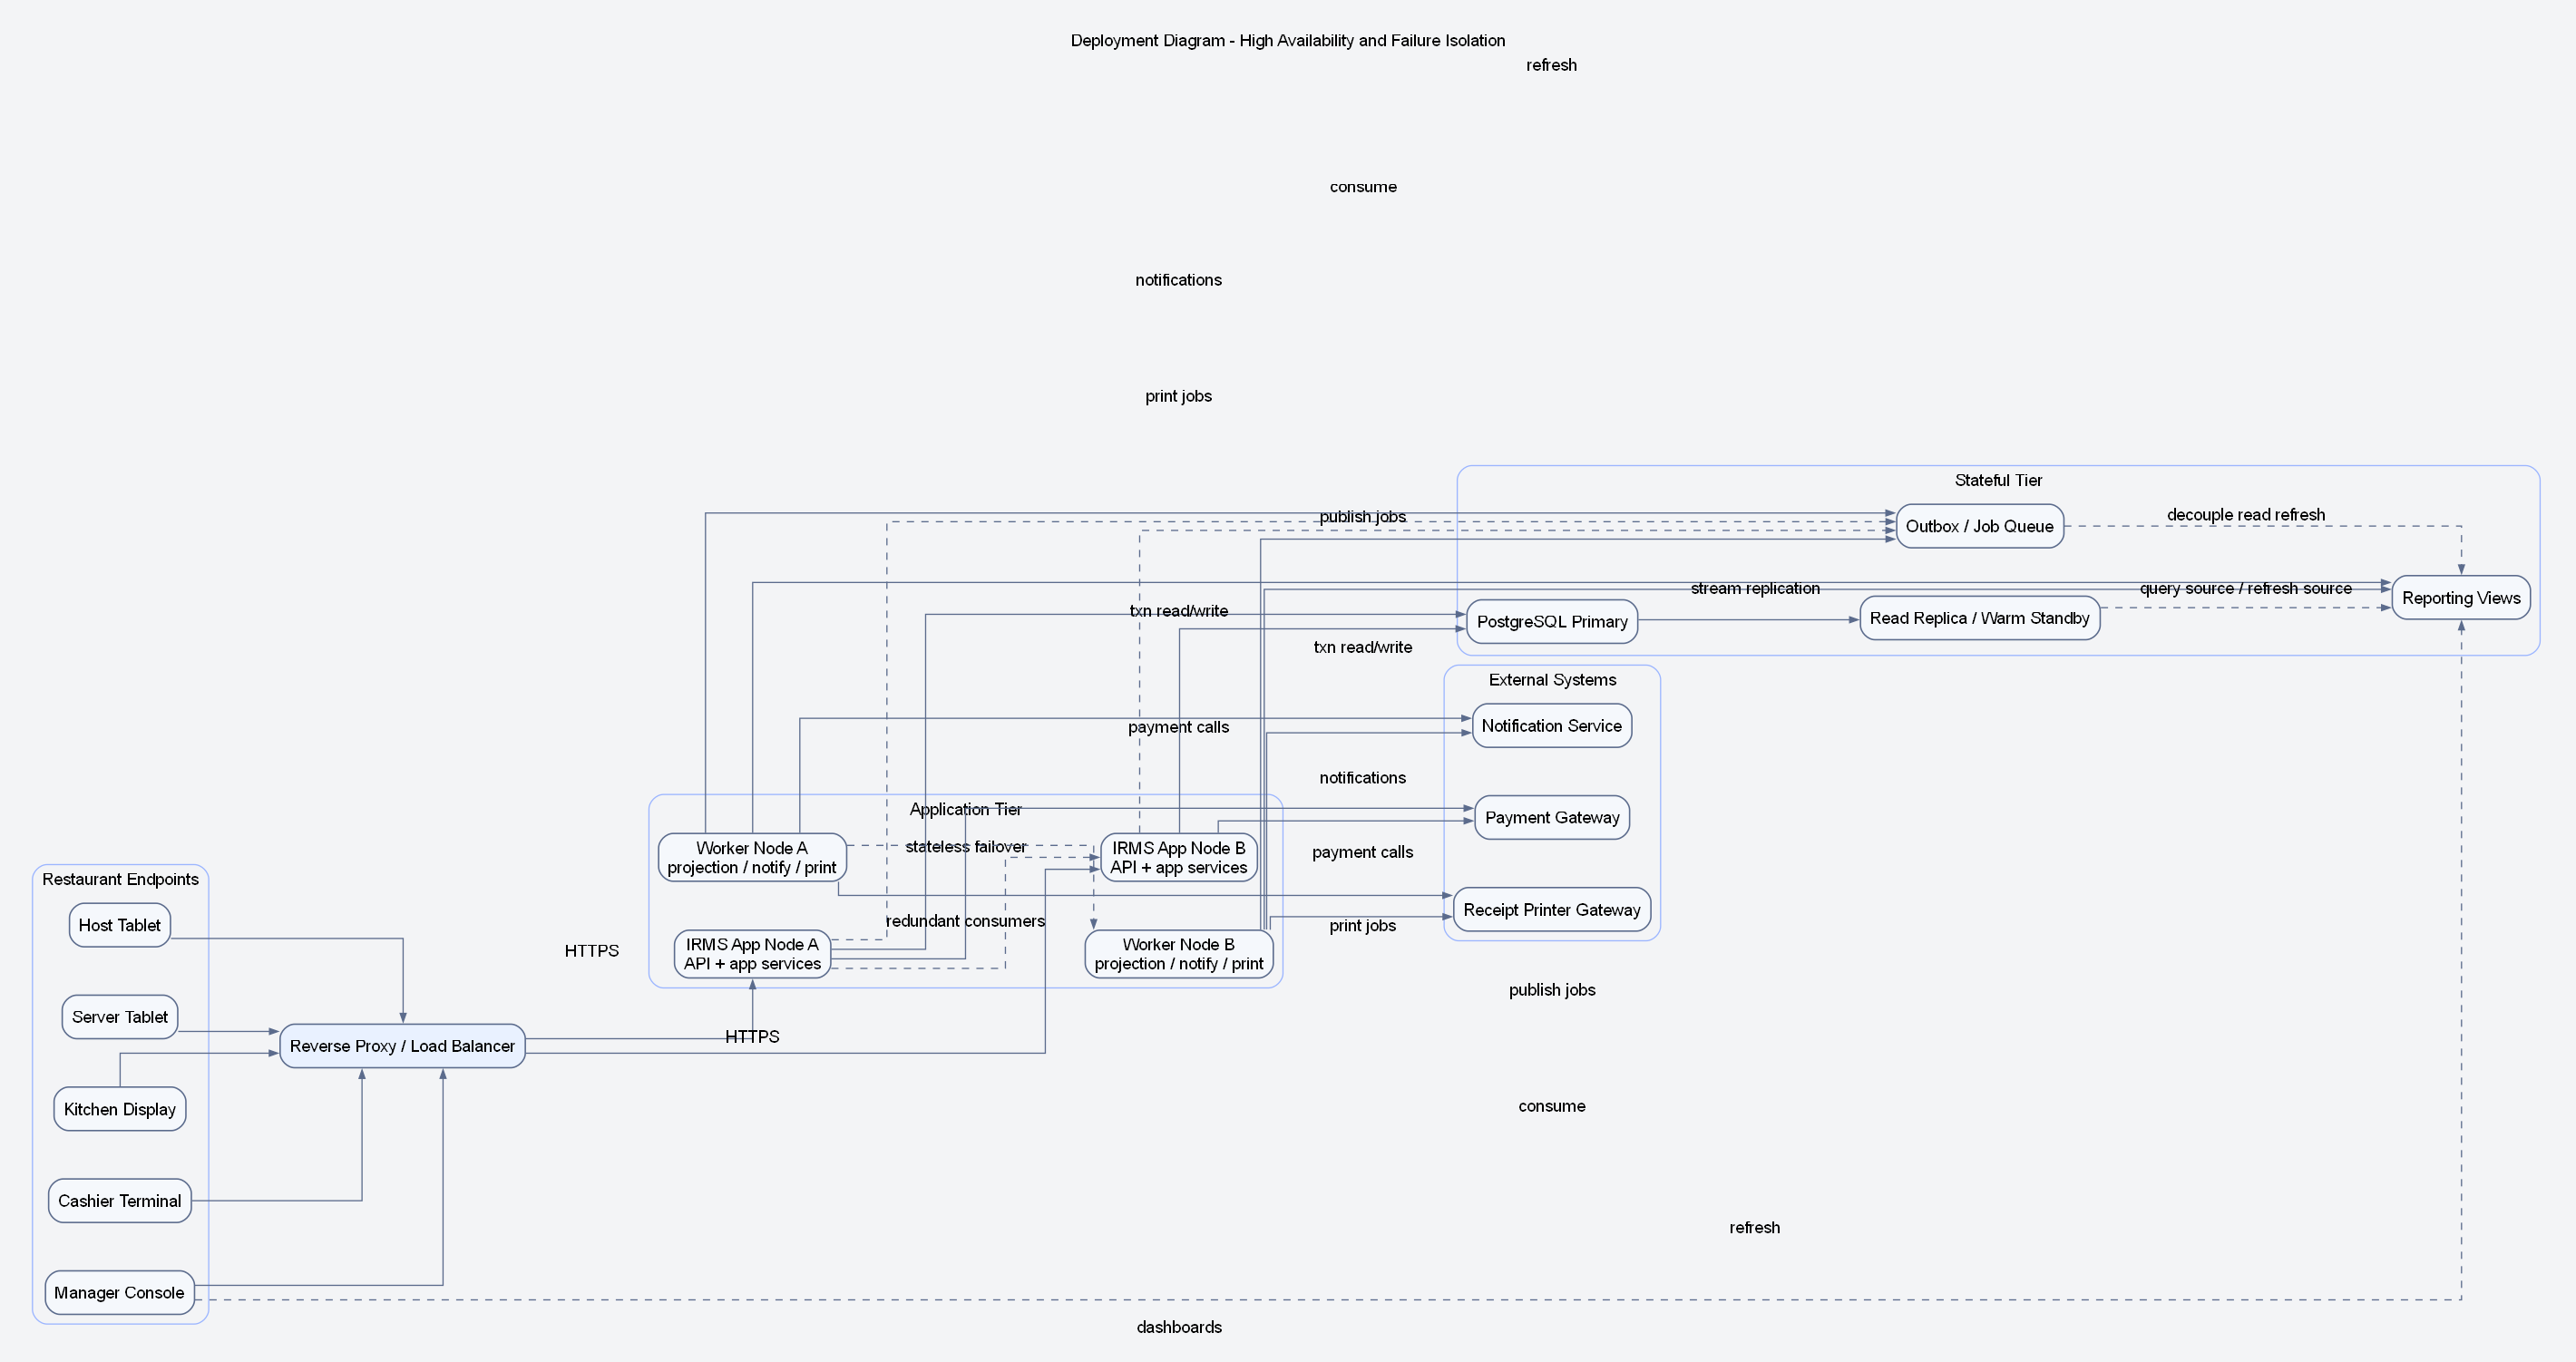
\includegraphics[width=0.97\linewidth,height=0.84\textheight,keepaspectratio]{32_deployment_diagram_high_availability_and_failure_isolation.png}
  }{
    \fbox{\parbox{0.82\linewidth}{Thiếu file \textsf{32\_deployment\_diagram\_high\_availability\_and\_failure\_isolation.(pdf/png)}.}}
  }
}
\caption{Sơ đồ triển khai cho runtime Docker local và cô lập lỗi}
\label{fig:irms-deployment-ha-supplement}
\end{figure}

Hình~\ref{fig:irms-deployment-ha-supplement} mô tả môi trường runtime thực tế qua \textsf{Docker Compose}, tập trung vào cấu trúc container, luồng sự kiện và cơ chế cô lập lỗi (fault isolation). 

\begin{itemize}
    \item \textbf{Luồng Request:} Request từ \textsf{frontend container} (React/Node.js) đi qua \textsf{api-gateway} (sử dụng \textsf{GatewayProxyController}) để định tuyến REST đến các service Spring Boot. Phạm vi triển khai hiện tại tập trung vào cụm container đơn, chưa bao gồm Load Balancing hay Failover.
    
    \item \textbf{Quản lý dữ liệu:} Dữ liệu lưu tại \textsf{PostgreSQL container} với volume \textsf{postgres-data}. \textsf{irms-migration} sử dụng Flyway để thực hiện migration trước khi khởi động các service nghiệp vụ. Hiện tại hệ thống dùng một instance vật lý duy nhất, chưa triển khai Replication hay Hot-standby.
    
    \item \textbf{Cô lập lỗi (Fault Isolation):} Tách biệt giao dịch lõi và các tác vụ phụ (side-effects). Giao dịch chính được xử lý đồng bộ; các tác vụ như cập nhật Read Model, gửi thông báo và ghi audit log được đẩy qua Outbox Pattern (\textsf{outbox\_events}, \textsf{processed\_events}) và \textsf{RabbitMQ}. Cơ chế này đảm bảo sự cố tại các module hỗ trợ không làm gián đoạn luồng nghiệp vụ chính tại nhà hàng.
    
    \item \textbf{Xử lý kịch bản lỗi:}
    \begin{itemize}
        \item \textsf{Gateway/Service} lỗi: Endpoint tương ứng sẽ ngừng hoạt động dựa trên healthcheck của Docker.
        \item Bộ xử lý nền lỗi: Sự kiện được lưu giữ trong Outbox table hoặc hàng đợi \textsf{RabbitMQ} để retry theo cấu hình.
        \item Side-effect chậm: Không block luồng giao dịch chính; ưu tiên hoàn tất thanh toán và chốt đơn trước.
    \end{itemize}
    
    \item \textbf{Suy giảm dịch vụ (Graceful Degradation):} Kiến trúc cho phép hệ thống duy trì hoạt động phần lõi khi các thành phần phụ gặp sự cố. Việc chấp nhận suy giảm có kiểm soát (chậm báo cáo/thông báo) giúp hệ thống tránh khỏi lỗi dây chuyền (cascading failure).
\end{itemize}
\paragraph{Mô tả}
\begin{itemize}
  \item \textbf{frontend container} tách giao diện React và proxy \textsf{/api} khỏi các service backend.
  \item \textbf{api-gateway} định tuyến REST đến các container service Spring Boot theo cấu hình thật.
  \item \textbf{PostgreSQL container} lưu dữ liệu giao dịch và các nhóm bảng hỗ trợ báo cáo trong một cơ sở dữ liệu vật lý duy nhất.
  \item \textbf{RabbitMQ container} cùng \textsf{outbox\_events} và \textsf{processed\_events} ngăn các tác vụ nền làm nghẽn trực tiếp tuyến giao dịch.
  \item \textbf{Reporting tables and views} cho phép tách nhu cầu đọc báo cáo khỏi phần xử lý lệnh nghiệp vụ.
\end{itemize}



Ngoài khả năng cô lập lỗi, sơ đồ cũng thể hiện rõ hướng mở rộng của hệ thống. Việc bổ sung thêm nút ứng dụng hoặc bộ xử lý nền có thể được thực hiện về sau, nhưng trong tài liệu hiện tại cần phân biệt rõ giữa cấu hình đã có trong \textsf{docker-compose.yml} và phương án mở rộng tương lai.

\subsubsection{Install View cho gói triển khai Docker local}

Deployment View ở trên trả lời các container và node runtime được đặt ở đâu. Install View dưới đây bổ sung góc nhìn còn lại: artifact, cấu hình và migration nào được đóng gói vào từng container khi chạy theo \textsf{Docker Compose}. Phần này chỉ mô tả runtime hiện tại, không bổ sung các hạ tầng như Kubernetes, dịch vụ đám mây, cân bằng tải, bản sao đọc dữ liệu hoặc nhà cung cấp ngoài khi chưa thuộc phạm vi triển khai.

\begin{figure}[H]
\centering
\IfFileExists{37_install_view_docker_local_artifacts.pdf}{
  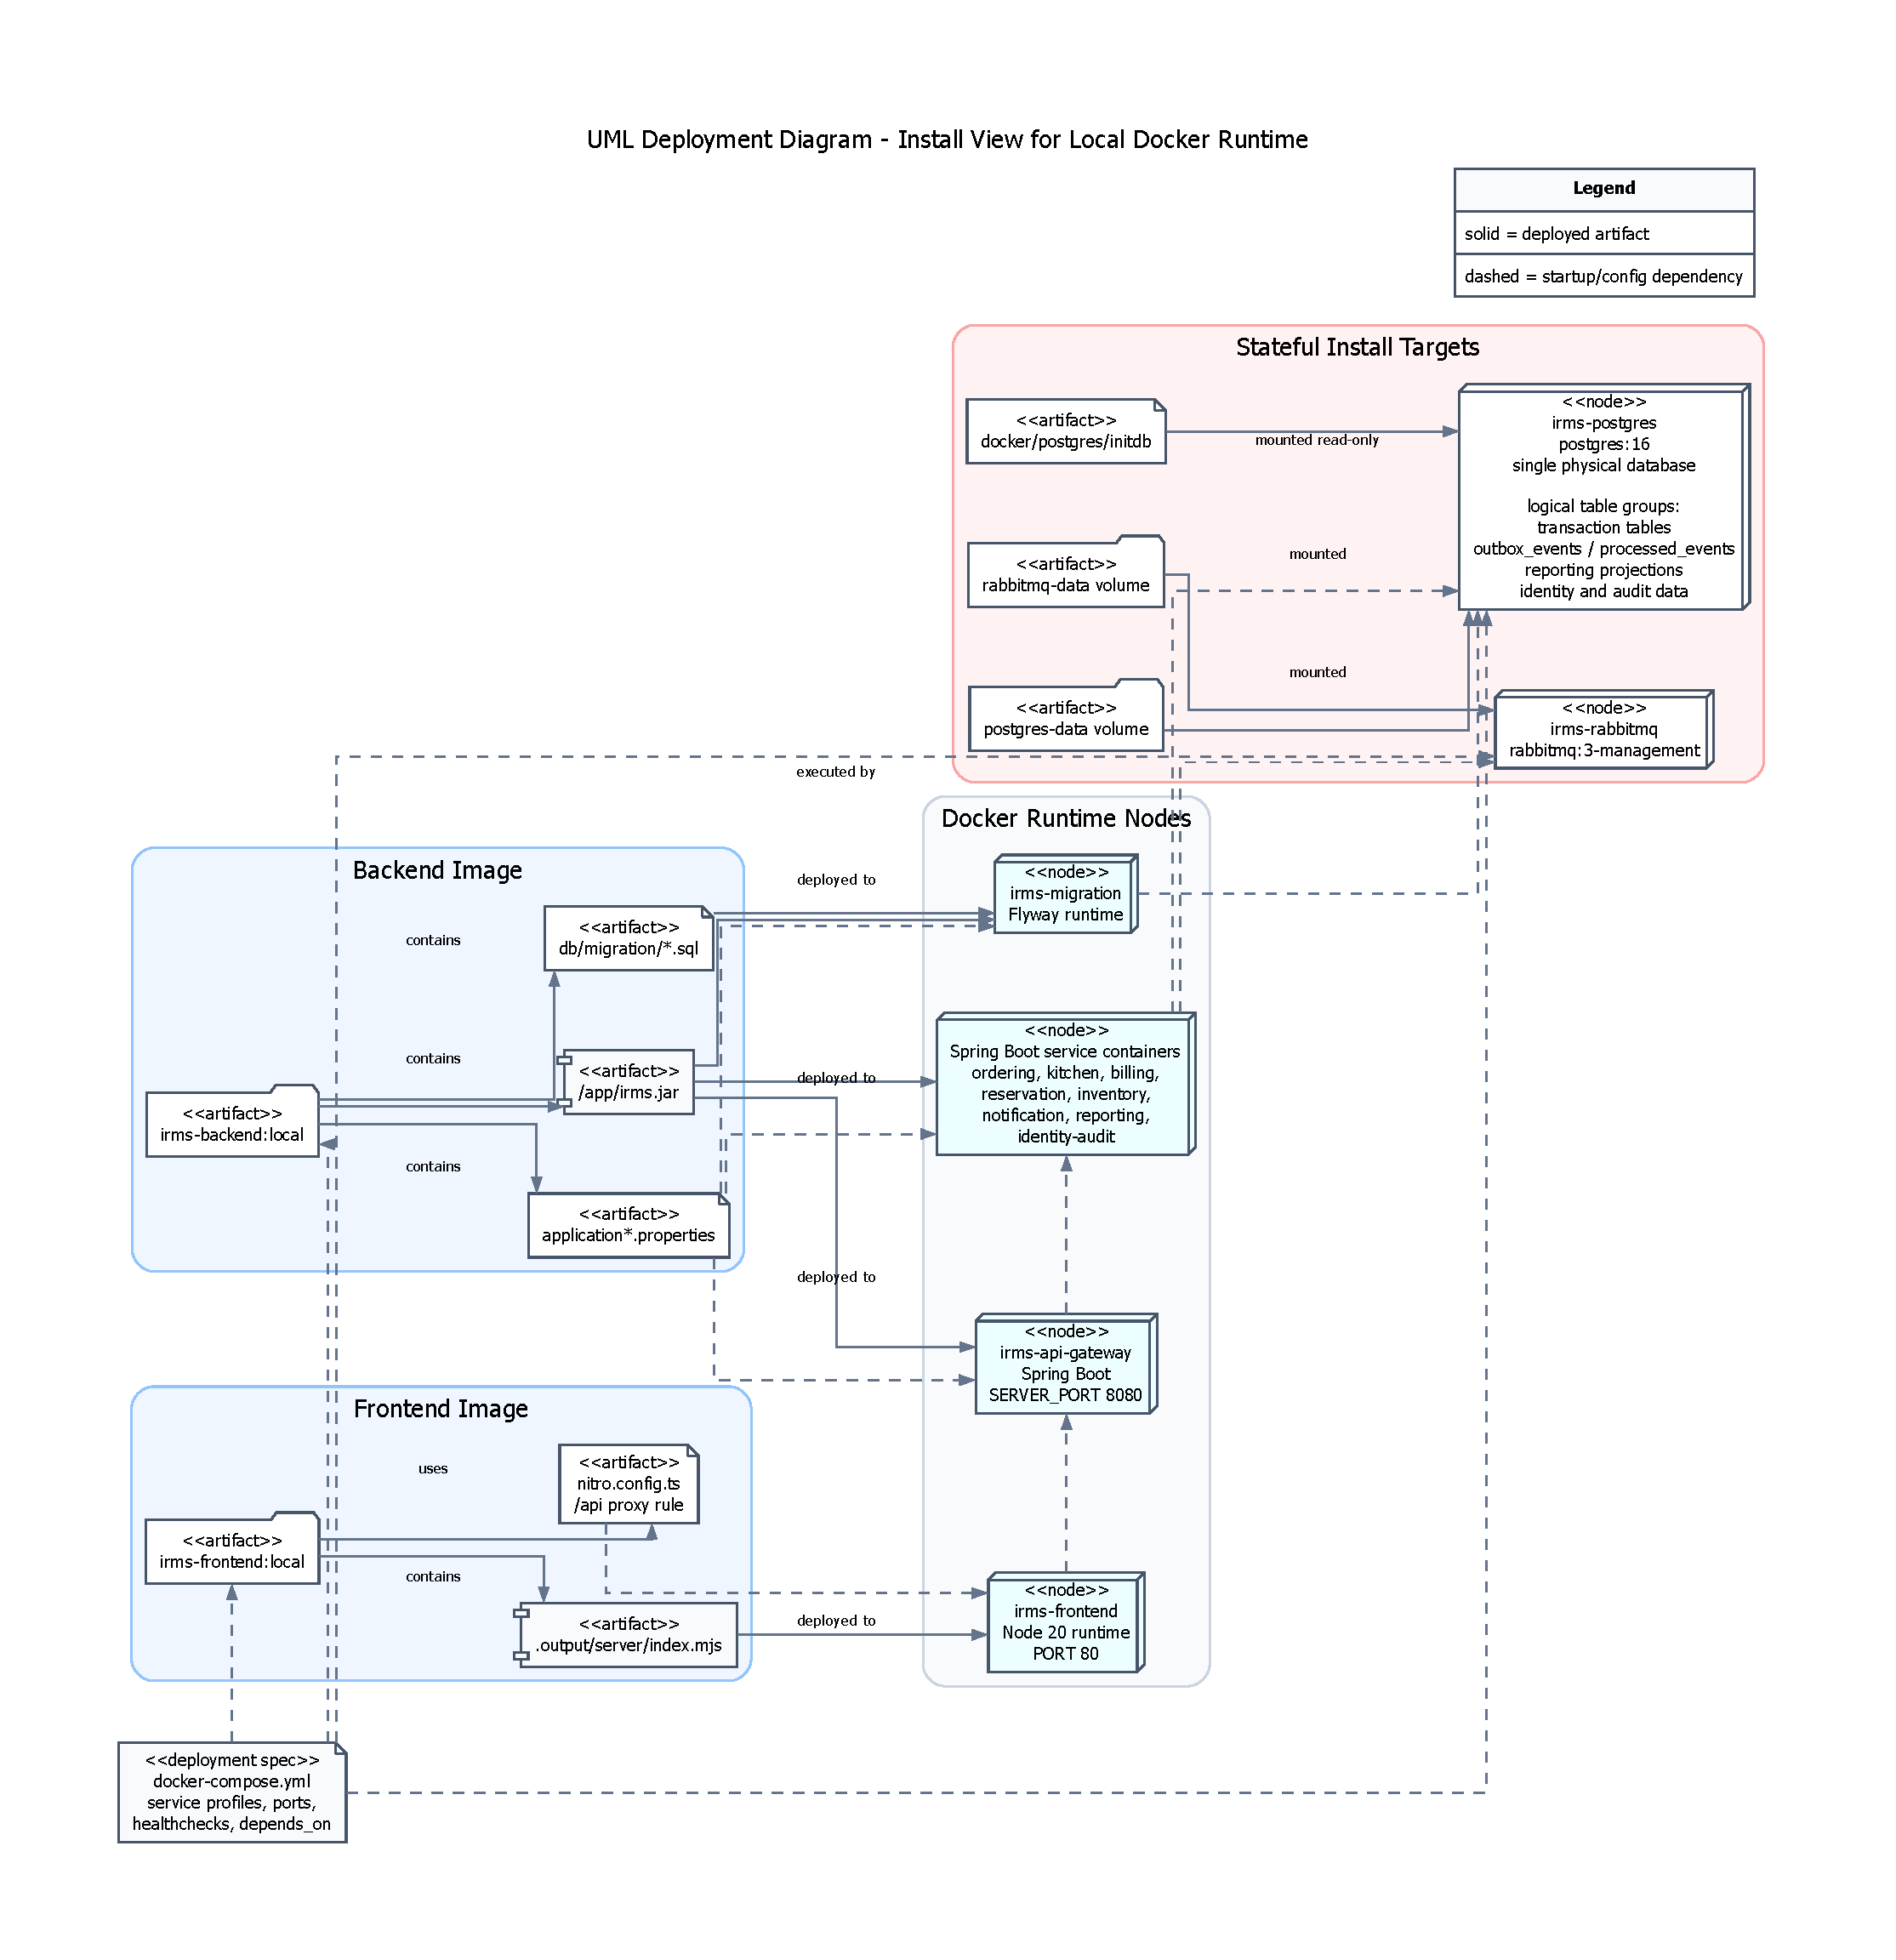
\includegraphics[width=0.97\linewidth,height=0.84\textheight,keepaspectratio]{37_install_view_docker_local_artifacts.pdf}
}{
  \IfFileExists{37_install_view_docker_local_artifacts.png}{
    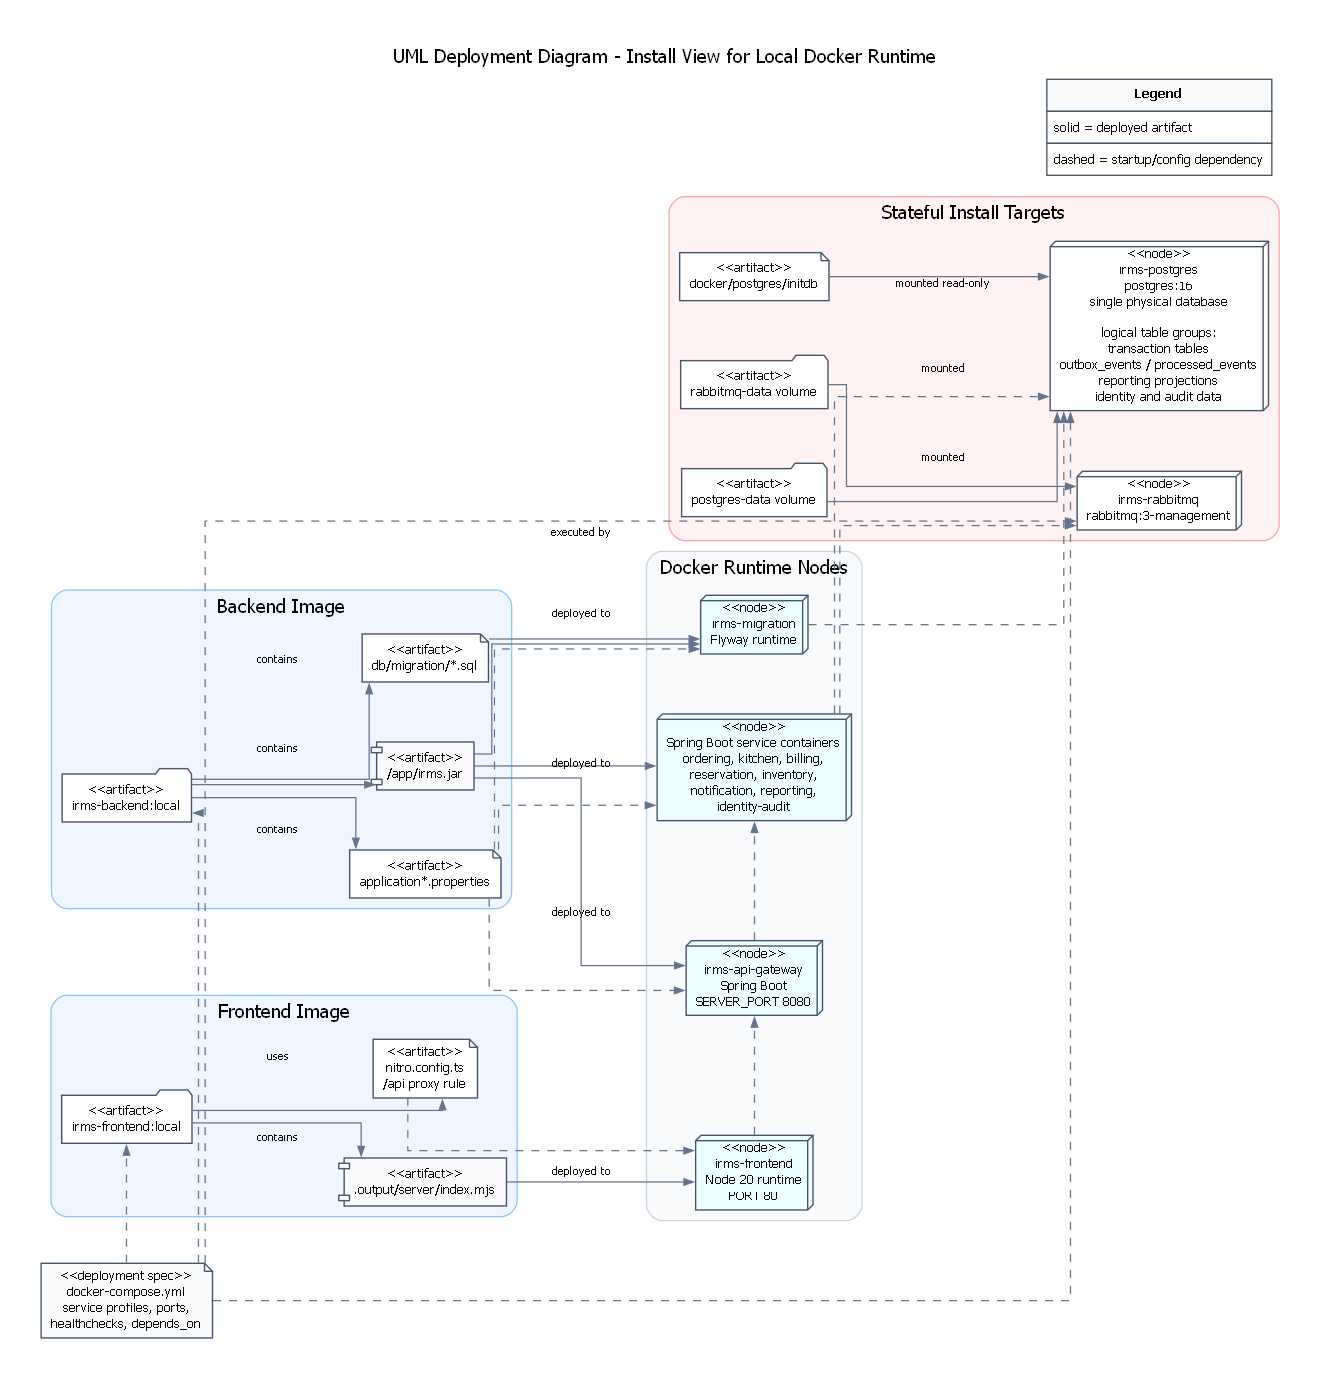
\includegraphics[width=0.97\linewidth,height=0.84\textheight,keepaspectratio]{37_install_view_docker_local_artifacts.png}
  }{
    \fbox{\parbox{0.82\linewidth}{Thiếu file \textsf{37\_install\_view\_docker\_local\_artifacts.(pdf/png)}.}}
  }
}

\caption{UML Deployment Diagram cho Install View của gói Docker local}
\label{fig:irms-install-view-docker-local}
\end{figure}

Hình~\ref{fig:irms-install-view-docker-local} dùng UML Deployment Diagram để thể hiện các node runtime và artifact cài đặt của gói Docker local. \textsf{irms-backend:local} chứa \textsf{/app/irms.jar}, các file \textsf{application*.properties} và migration SQL; cùng artifact JAR này được triển khai vào \textsf{api-gateway}, các service Spring Boot và \textsf{irms-migration}, nhưng vai trò runtime khác nhau nhờ profile và biến môi trường trong \textsf{docker-compose.yml}. \textsf{irms-frontend:local} chứa bundle Nitro ở \textsf{.output/server/index.mjs}; \textsf{nitro.config.ts} điều khiển proxy \textsf{/api/**} sang \textsf{api-gateway}. Các node trạng thái chỉ gồm \textsf{PostgreSQL} với \textsf{postgres-data} và \textsf{RabbitMQ} với \textsf{rabbitmq-data}, đúng với cấu hình hiện tại.

\begin{table}[H]
\centering
\footnotesize
\renewcommand{\arraystretch}{1.15}
\caption{Install View cho artifact backend và frontend}
\label{tab:irms-install-view}
\begin{tabularx}{\textwidth}{>{\raggedright\arraybackslash}p{0.19\linewidth} >{\raggedright\arraybackslash}p{0.36\linewidth} >{\raggedright\arraybackslash}X}
\toprule
\textbf{Artifact/config item} & \textbf{Nơi sử dụng} & \textbf{Vai trò runtime} \\
\midrule
Backend Spring Boot artifact \textsf{irms.jar} & \texttt{backend/Dockerfile}; \texttt{backend/pom.xml}; \texttt{docker-compose.yml}. & Image \textsf{irms-backend:local} được dùng lại cho \textsf{api-gateway}, các service nghiệp vụ và \textsf{irms-migration}. Vai trò service được chọn bằng \texttt{SPRING\_PROFILES\_ACTIVE}, \texttt{IRMS\_RUNTIME\_SERVICE} và \texttt{SERVER\_PORT}. \\
Migration runtime và SQL migrations & Giai đoạn khởi tạo schema dữ liệu. & Container \textsf{irms-migration} chạy Flyway trước service nghiệp vụ, với điều kiện \texttt{service\_completed\_successfully}. \\
Frontend bundle / Nitro server & \texttt{frontend/Dockerfile}; \texttt{frontend/package.json}; \texttt{frontend/nitro.config.ts}. & Image \textsf{irms-frontend:local} chạy \texttt{node .output/server/index.mjs}, phục vụ UI React/TanStack và proxy \textsf{/api/**} tới \textsf{api-gateway}. \\
Runtime application properties & \texttt{application.properties}; \texttt{application-docker.properties}; \texttt{application-\char`*-service.properties}. & Cấu hình datasource PostgreSQL, RabbitMQ, Flyway, CORS, security token, timeout phiên, outbox và URL service nội bộ. \\
\bottomrule
\end{tabularx}
\end{table}

\begin{table}[H]
\centering
\scriptsize
\renewcommand{\arraystretch}{1.15}
\setlength{\tabcolsep}{2pt}
\caption{Install View cho thành phần trạng thái và cấu hình Docker}
\label{tab:irms-install-stateful-view}
\begin{tabularx}{\textwidth}{>{\raggedright\arraybackslash}p{0.19\linewidth} >{\raggedright\arraybackslash}p{0.36\linewidth} >{\raggedright\arraybackslash}X}
\toprule
\textbf{Thành phần} & \textbf{Nơi sử dụng} & \textbf{Vai trò runtime} \\
\midrule
\textsf{irms-postgres} và \textsf{postgres-data} & \texttt{docker-compose.yml}; \texttt{docker/postgres/initdb}. & Một PostgreSQL container vật lý duy nhất lưu dữ liệu giao dịch, \textsf{outbox\_events}, \textsf{processed\_events}, các bảng projection báo cáo và dữ liệu identity/audit trong cùng PostgreSQL; các nhóm này không phải database riêng. \\
\textsf{irms-rabbitmq} và \textsf{rabbitmq-data} & \texttt{docker-compose.yml}; \texttt{application.properties}; \texttt{application-docker.properties}. & Broker cho tuyến event-driven; các service dùng \texttt{spring.rabbitmq.*}, manual ack và publisher confirm khi \texttt{IRMS\_RABBITMQ\_ENABLED=true}. \\
Thứ tự khởi động Docker & \texttt{depends\_on} và healthcheck trong \texttt{docker-compose.yml}. & \textsf{postgres} và \textsf{rabbitmq} healthy trước, \textsf{irms-migration} hoàn tất, sau đó Spring Boot services chạy và cuối cùng frontend phụ thuộc \textsf{api-gateway}. \\
\bottomrule
\end{tabularx}
\end{table}

Bảng thể hiện thứ tự cài đặt/khởi động của phạm vi triển khai hiện tại: \textsf{postgres} và \textsf{rabbitmq} phải healthy trước, \textsf{irms-migration} chạy thành công để tạo/cập nhật schema, sau đó các service Spring Boot và cuối cùng là \textsf{frontend} phụ thuộc vào \textsf{api-gateway}. Đây là Install View của runtime Docker local hiện có, không phải mô tả triển khai cloud hay cụm sẵn sàng cao.

\subsection{Nguyên tắc thiết kế}\label{sec:architecture-principles}
Kiến trúc của IRMS bám theo các nguyên tắc thiết kế sau:
\begin{itemize}
  \item \textbf{High Cohesion, Low Coupling:} Mỗi service chỉ expose API, event và data contract cần thiết; ẩn hoàn toàn chi tiết triển khai (encapsulation).
  \item \textbf{Separation of Concerns (SoC):} Tách biệt rõ rệt vai trò giữa Controller, Application Service, Domain và Infrastructure.
  \item \textbf{Dependency Inversion:} Domain core chỉ phụ thuộc vào abstraction (interface); các adapter hạ tầng phụ thuộc ngược lại vào core, tránh gắn chặt vào library hoặc provider cụ thể.
  \item \textbf{Synchronous API (Core Transactions):} Xử lý đồng bộ các nghiệp vụ cần phản hồi tức thời như đặt bàn, gọi món và thanh toán để đảm bảo tính nhất quán trạng thái.
  \item \textbf{Asynchronous Events (Side-effects):} Các tác vụ phụ như cảnh báo kho, cập nhật báo cáo, thông báo và audit log được xử lý bất đồng bộ qua Outbox Pattern và Event Bus.
  \item \textbf{Domain-centric Modeling:} Tập trung mô hình hóa hành vi nghiệp vụ thực tế (Domain Behavior) thay vì thiết kế dựa trên quan hệ dữ liệu (Database-centric) thuần túy.
\end{itemize}

\subsection{Áp dụng nguyên lý SOLID vào thiết kế}\label{sec:solid-design}

Phần này đối chiếu trực tiếp các nguyên tắc SOLID với thiết kế thực tế (implementation) của IRMS qua các class và interface tiêu biểu, thay vì liệt kê lý thuyết đơn thuần. Các interface như \textsf{PaymentGateway}, \textsf{NotificationChannelAdapter} và \textsf{ReceiptDeliveryAdapter} cụ thể hóa quyết định dùng boundary adapters trong \adrref{ADR-0011}{adr:0011-boundary-adapters}; cách tách lớp \texttt{api}, \texttt{application}, \texttt{domain} và \texttt{infrastructure} liên kết với \adrref{ADR-0013}{adr:0013-service-layering}.

\begin{table}[H]
\centering
\footnotesize
\renewcommand{\arraystretch}{1.15}
\caption{Đối chiếu nguyên tắc SOLID với thiết kế IRMS}
\label{tab:solid-thiết kế-evidence}
\begin{tabularx}{\textwidth}{>{\raggedright\arraybackslash}p{0.13\linewidth} >{\raggedright\arraybackslash}X >{\raggedright\arraybackslash}X}
\toprule
\textbf{Nguyên tắc} & \textbf{Ví dụ thiết kế tiêu biểu} & \textbf{Ý nghĩa thiết kế} \\
\midrule
SRP & \texttt{BillingPaymentService}; \texttt{BillingReceiptService}; \texttt{KitchenTicketTransitionPolicy}; \texttt{ManualAckConsumerSupport}; \texttt{RabbitMqOutboxRelay}. & Trách nhiệm được tách theo service, policy, adapter và consumer; khi thay đổi thanh toán, trạng thái bếp hoặc retry RabbitMQ, phạm vi sửa được khoanh vào nhóm class đúng vai trò. \\
OCP & \texttt{PaymentGateway} với \texttt{CashPaymentGateway}, \texttt{ExternalReferencePaymentGateway}; \texttt{BillSplitStrategy} với các strategy chia hóa đơn; \texttt{ReorderRecommendationStrategy}. & Các điểm dễ thay đổi được mở qua interface/strategy/policy, nên có thể thêm biến thể mới bằng class hiện thực mới và cấu hình bean. \\
LSP & \texttt{BillingPaymentService} nhận \texttt{List<PaymentGateway>} và gọi \texttt{supports(...)}; \texttt{BillingSplitService} nhận \texttt{List<BillSplitStrategy>}. & Service sử dụng contract ổn định; implementation có thể thay thế trong phạm vi hợp đồng đã định nghĩa. \\
ISP & \texttt{PaymentGateway}; \texttt{ReceiptDeliveryAdapter}; \texttt{NotificationChannelAdapter}; \texttt{KitchenTicketItemRepositoryPort}; \texttt{DomainEventPublisher}. & Interface được giữ nhỏ và gắn với một vai trò cụ thể, giúp client chỉ phụ thuộc vào hành vi nó thật sự cần. \\
DIP & \texttt{BillingPaymentService} phụ thuộc \texttt{BillPaymentRepository}, \texttt{PaymentGateway}, \texttt{DomainEventPublisher}; \texttt{BillingReceiptService} phụ thuộc \texttt{ReceiptDeliveryAdapter}; \texttt{JdbcKitchenTicketItemRepository} implements \texttt{KitchenTicketItemRepositoryPort}. & Service cấp cao phụ thuộc abstraction/port, còn hạ tầng hiện thực chi tiết JDBC, RabbitMQ hoặc adapter kênh. \\
\bottomrule
\end{tabularx}
\end{table}

\paragraph{Thanh toán và biên nhận.}
\textsf{BillingPaymentService} không biết chi tiết xử lý từng phương thức thanh toán, mà làm việc qua \textsf{PaymentGateway}. Các hiện thực như \textsf{CashPaymentGateway} và \textsf{ExternalReferencePaymentGateway} được xem là adapter thanh toán ở biên. Tương tự, \textsf{BillingReceiptService} phát hành biên nhận qua \textsf{ReceiptDeliveryAdapter} với \textsf{DigitalReceiptDeliveryAdapter} và \textsf{PrintReceiptDeliveryAdapter}. Đây là ví dụ mạnh cho OCP, ISP và DIP: service lõi giữ luồng thanh toán, còn biến thể phương thức/kênh nằm ở lớp hiện thực.

\paragraph{Thông báo.}
Nhóm \textsf{NotificationChannelAdapter} được tách thành các kênh nhỏ, gồm:
\begin{itemize}
  \item \textsf{EmailNotificationChannelAdapter}, \textsf{SmsNotificationChannelAdapter};
  \item \textsf{InAppNotificationChannelAdapter}, \textsf{PrintNotificationChannelAdapter};
  \item \textsf{PhoneNotificationChannelAdapter}.
\end{itemize}
Những class này giúp service thông báo kiểm tra và ghi nhận kênh gửi mà không biến phần notification thành một interface quá lớn. Các adapter này được mô tả như điểm mở rộng nội bộ cho các kênh gửi, không làm lõi thông báo phụ thuộc trực tiếp vào một kênh cụ thể.

\paragraph{Policy và strategy nghiệp vụ.}
\textsf{DomainPolicyConfiguration} đăng ký các nhóm policy/strategy như:
\begin{itemize}
  \item \textsf{OrderStatusPolicy}, \textsf{ComboPricingPolicy};
  \item \textsf{KitchenTicketTransitionPolicy}, \textsf{KitchenDeadlinePolicy};
  \item \textsf{LowStockSeverityPolicy}, \textsf{ReorderRecommendationStrategy};
  \item các hiện thực \textsf{BillSplitStrategy}.
\end{itemize}
Cách tách này làm rõ SRP: quy tắc chuyển trạng thái, tính deadline, đề xuất nhập hàng hoặc tách hóa đơn không bị trộn vào controller. Đồng thời, các strategy như \textsf{BillSplitStrategy} và \textsf{ReorderRecommendationStrategy} là điểm mở rộng OCP được thể hiện rõ trong thiết kế.

\paragraph{Outbox, RabbitMQ và bộ xử lý sự kiện nền.}
Ở tuyến event-driven, \textsf{TransactionalOutboxPublisher} hiện thực \textsf{DomainEventPublisher}, \textsf{RabbitMqOutboxRelay} phụ trách chuyển outbox sang RabbitMQ, còn \textsf{ManualAckConsumerSupport} gom logic ack, retry, deduplication và dead-letter cho consumer. Phần này là ví dụ SRP và DIP ở tầng hạ tầng: service nghiệp vụ chỉ publish event qua abstraction, còn cách phát, retry hoặc dead-letter nằm trong component kỹ thuật riêng.

\paragraph{Giới hạn cần tránh diễn giải quá mức.}
Các ví dụ trên cho thấy IRMS có áp dụng SOLID tại những điểm thiết kế chính, đặc biệt ở service, adapter, policy, strategy, port truy cập dữ liệu và event infrastructure. Điều đó không có nghĩa mọi class đều hoàn hảo theo SOLID. Ngoài ra, các interface như \textsf{PaymentGateway}, \textsf{ReceiptDeliveryAdapter} và \textsf{NotificationChannelAdapter} xác định ranh giới trừu tượng, không làm cho lõi nghiệp vụ phụ thuộc vào một kênh thanh toán, thông báo hoặc in ấn cụ thể.

\subsection{Khả năng mở rộng trong tương lai}
\begin{figure}[H]
\centering
\IfFileExists{36_future_extensibility_evolution_path.pdf}{
  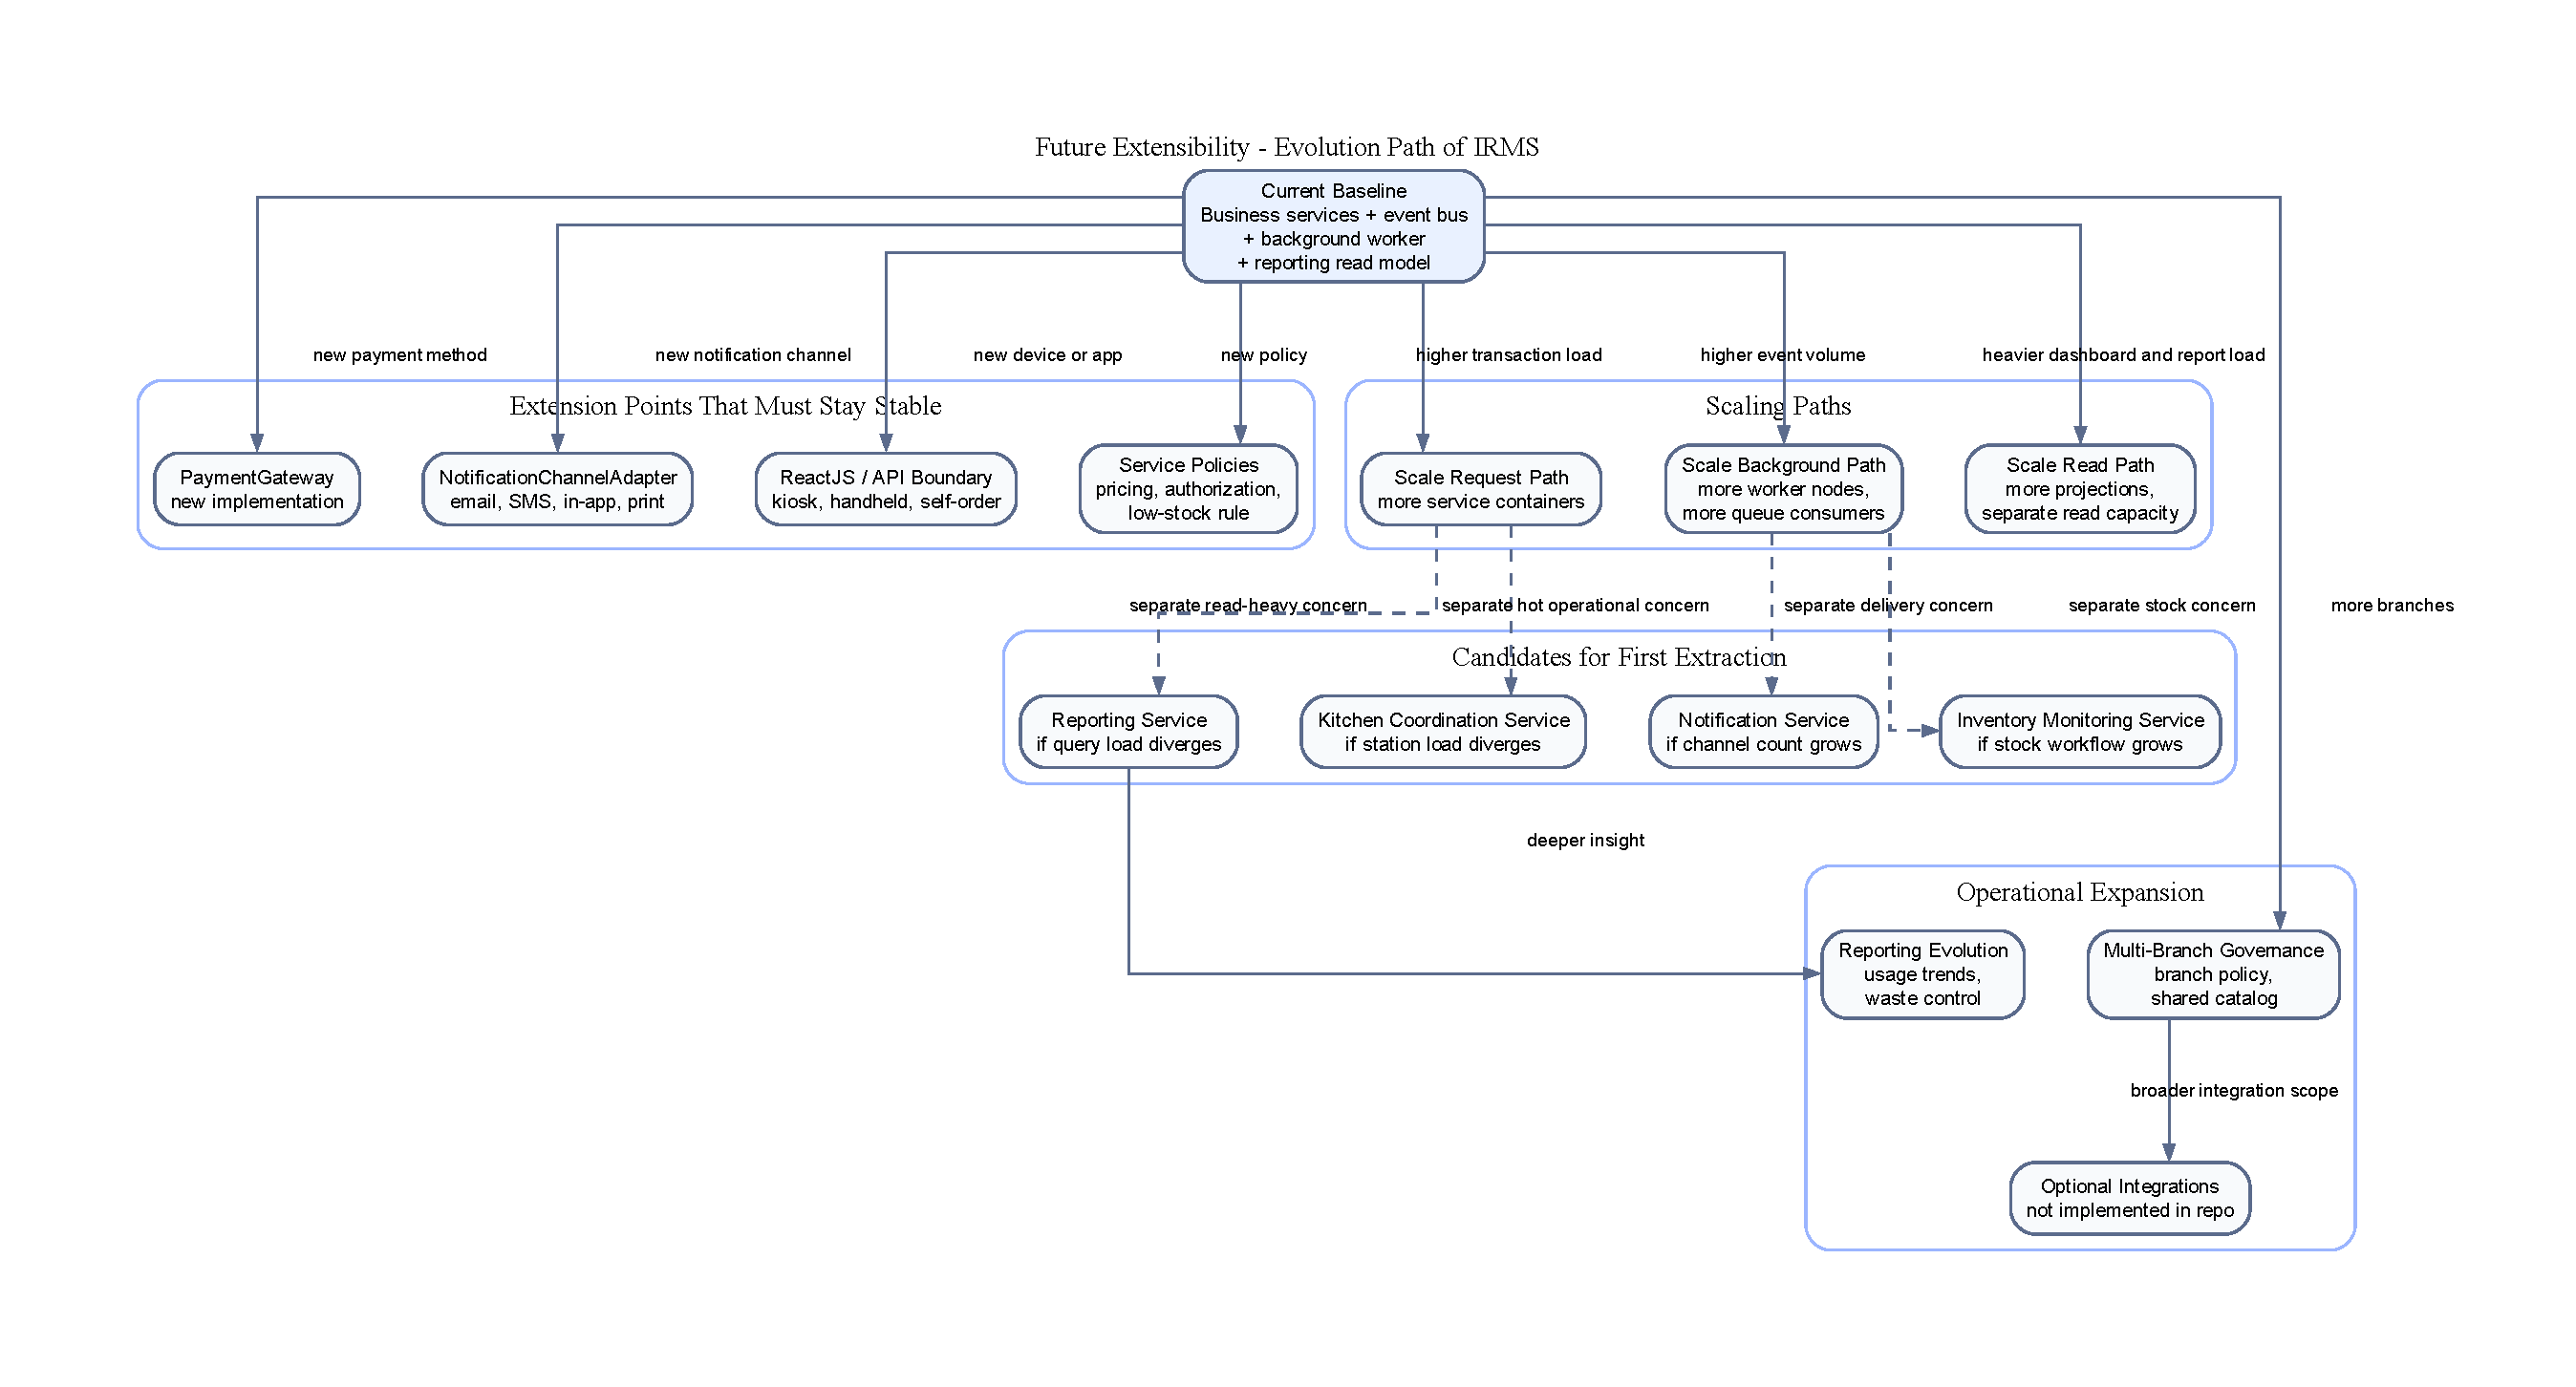
\includegraphics[width=\textwidth,height=0.82\textheight,keepaspectratio]{36_future_extensibility_evolution_path.pdf}
}{
  \IfFileExists{36_future_extensibility_evolution_path.png}{
    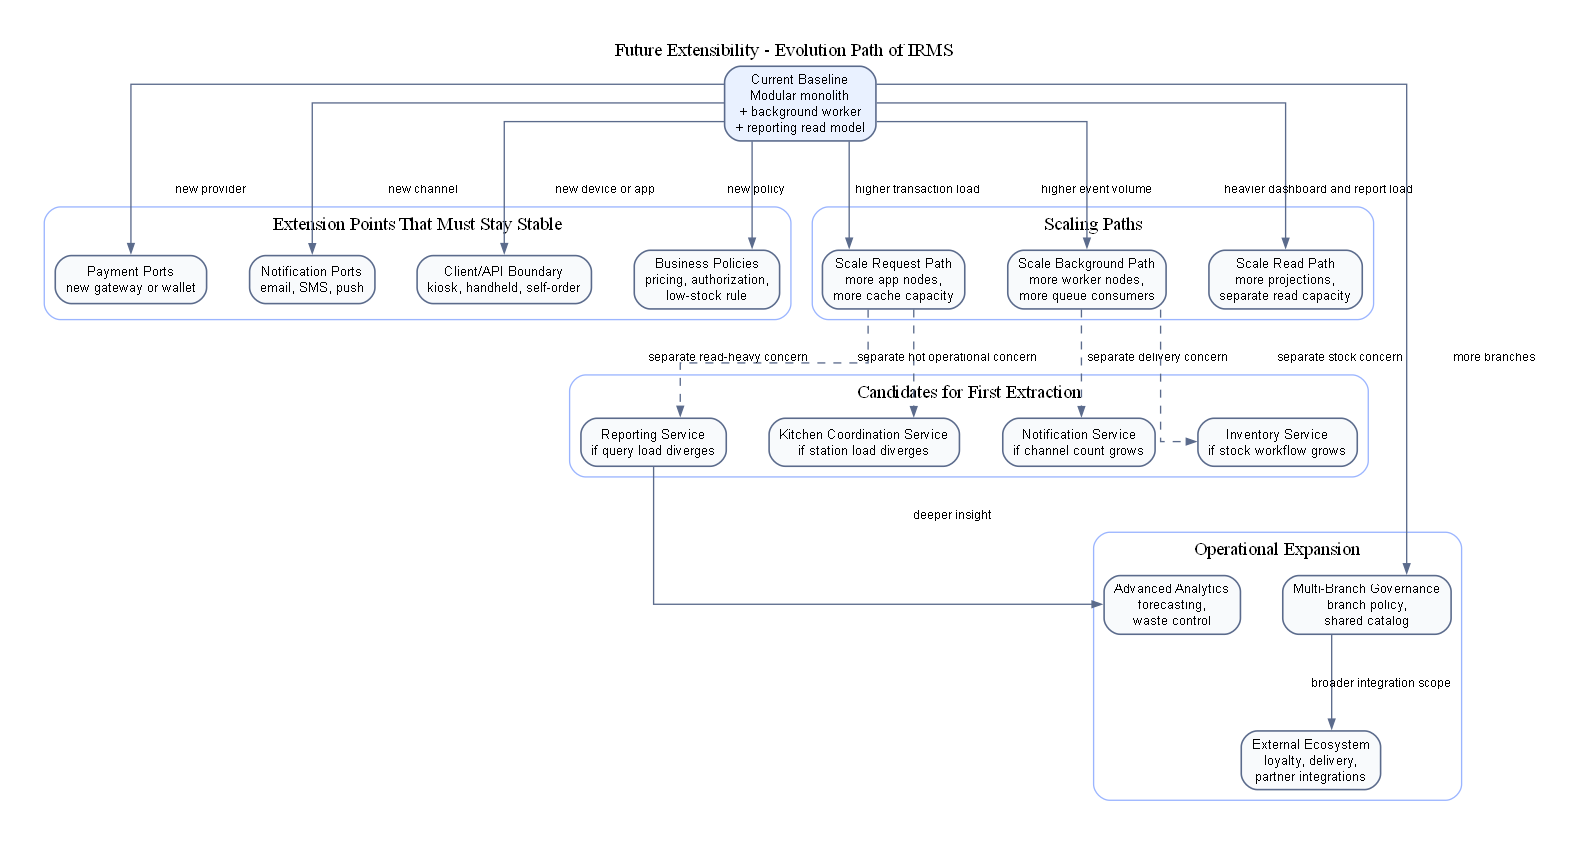
\includegraphics[width=\textwidth,height=0.82\textheight,keepaspectratio]{36_future_extensibility_evolution_path.png}
  }{
    \fbox{\parbox{0.82\linewidth}{Thiếu file \textsf{36\_future\_extensibility\_evolution\_path.(pdf/png)}.}}
  }
}
\caption{Lộ trình mở rộng kiến trúc của IRMS trong tương lai}
\label{fig:irms-future-extensibility}
\end{figure}

Hình~\ref{fig:irms-future-extensibility} mô tả lộ trình tiến hóa (evolutionary path) của hệ thống khi mở rộng quy mô (tăng thiết bị, chi nhánh, tích hợp) mà không cần tái cấu trúc tầng lõi (Core Domain). 

\paragraph{Trạng thái kiến trúc hiện tại:}
IRMS áp dụng mô hình SOA kết hợp Event-driven. Các nghiệp vụ chính (Core Transactions) sử dụng Sync API để đảm bảo tính nhất quán; các tác vụ phụ (Side-effects) được xử lý bất đồng bộ qua Event. Thiết kế này cho phép các service hỗ trợ như \textsf{Reporting}, \textsf{Notification}, \textsf{Inventory} có thể scale độc lập tùy theo tải trọng thực tế.

\paragraph{Nguyên tắc mở rộng không phá vỡ kiến trúc:}
Khả năng mở rộng (Extensibility) của IRMS được đo lường bằng việc duy trì sự ổn định của Core Domain (Order, Billing) khi thay đổi các thành phần biên:
\begin{itemize}
    \item \textbf{Tích hợp thanh toán/thông báo:} Chỉ tác động đến \textsf{PaymentGateway} và \textsf{NotificationChannelAdapter}.
    \item \textbf{Mở rộng quy mô:} Thêm chi nhánh hoặc thiết bị (Kiosk, Mobile) chỉ yêu cầu điều chỉnh tại tầng Deployment và API layer.
    \item \textbf{Điểm mở rộng chiến lược:} Các thành phần như Gateway, Adapter, Policy (quy tắc định giá/tồn kho) và Read Model cần được giữ ổn định để đảm bảo hệ thống tiến hóa có kiểm soát.
\end{itemize}

\paragraph{Các hướng mở rộng chính:}
\begin{itemize}
    \item \textbf{Mở rộng tích hợp (Integration):} Thêm Provider (thanh toán, thông báo) hoặc thiết bị ngoại vi qua mô hình Ports \& Adapters.
    \item \textbf{Mở rộng theo tải (Scaling):} Tăng số lượng instance ứng dụng, Background Worker hoặc tách biệt hoàn toàn Read Model để tối ưu truy vấn.
    \item \textbf{Mở rộng phạm vi vận hành:} Hỗ trợ đa chi nhánh và quản trị tập trung (Centralized Management) trên cùng một mô hình nghiệp vụ lõi.
    \item \textbf{Mở rộng theo dịch vụ:} Chỉ tách thành các Microservices độc lập đối với những vùng có nhịp thay đổi (rate of change) hoặc tải trọng khác biệt hoàn toàn.
\end{itemize}

\section{Thiết kế chi tiết}

\subsection{Góc nhìn lớp}
\label{sec:detailed-design-class-view}
\begin{figure}[H]
\centering
\IfFileExists{18_uml_class_diagram_core_domain_overview.pdf}{
  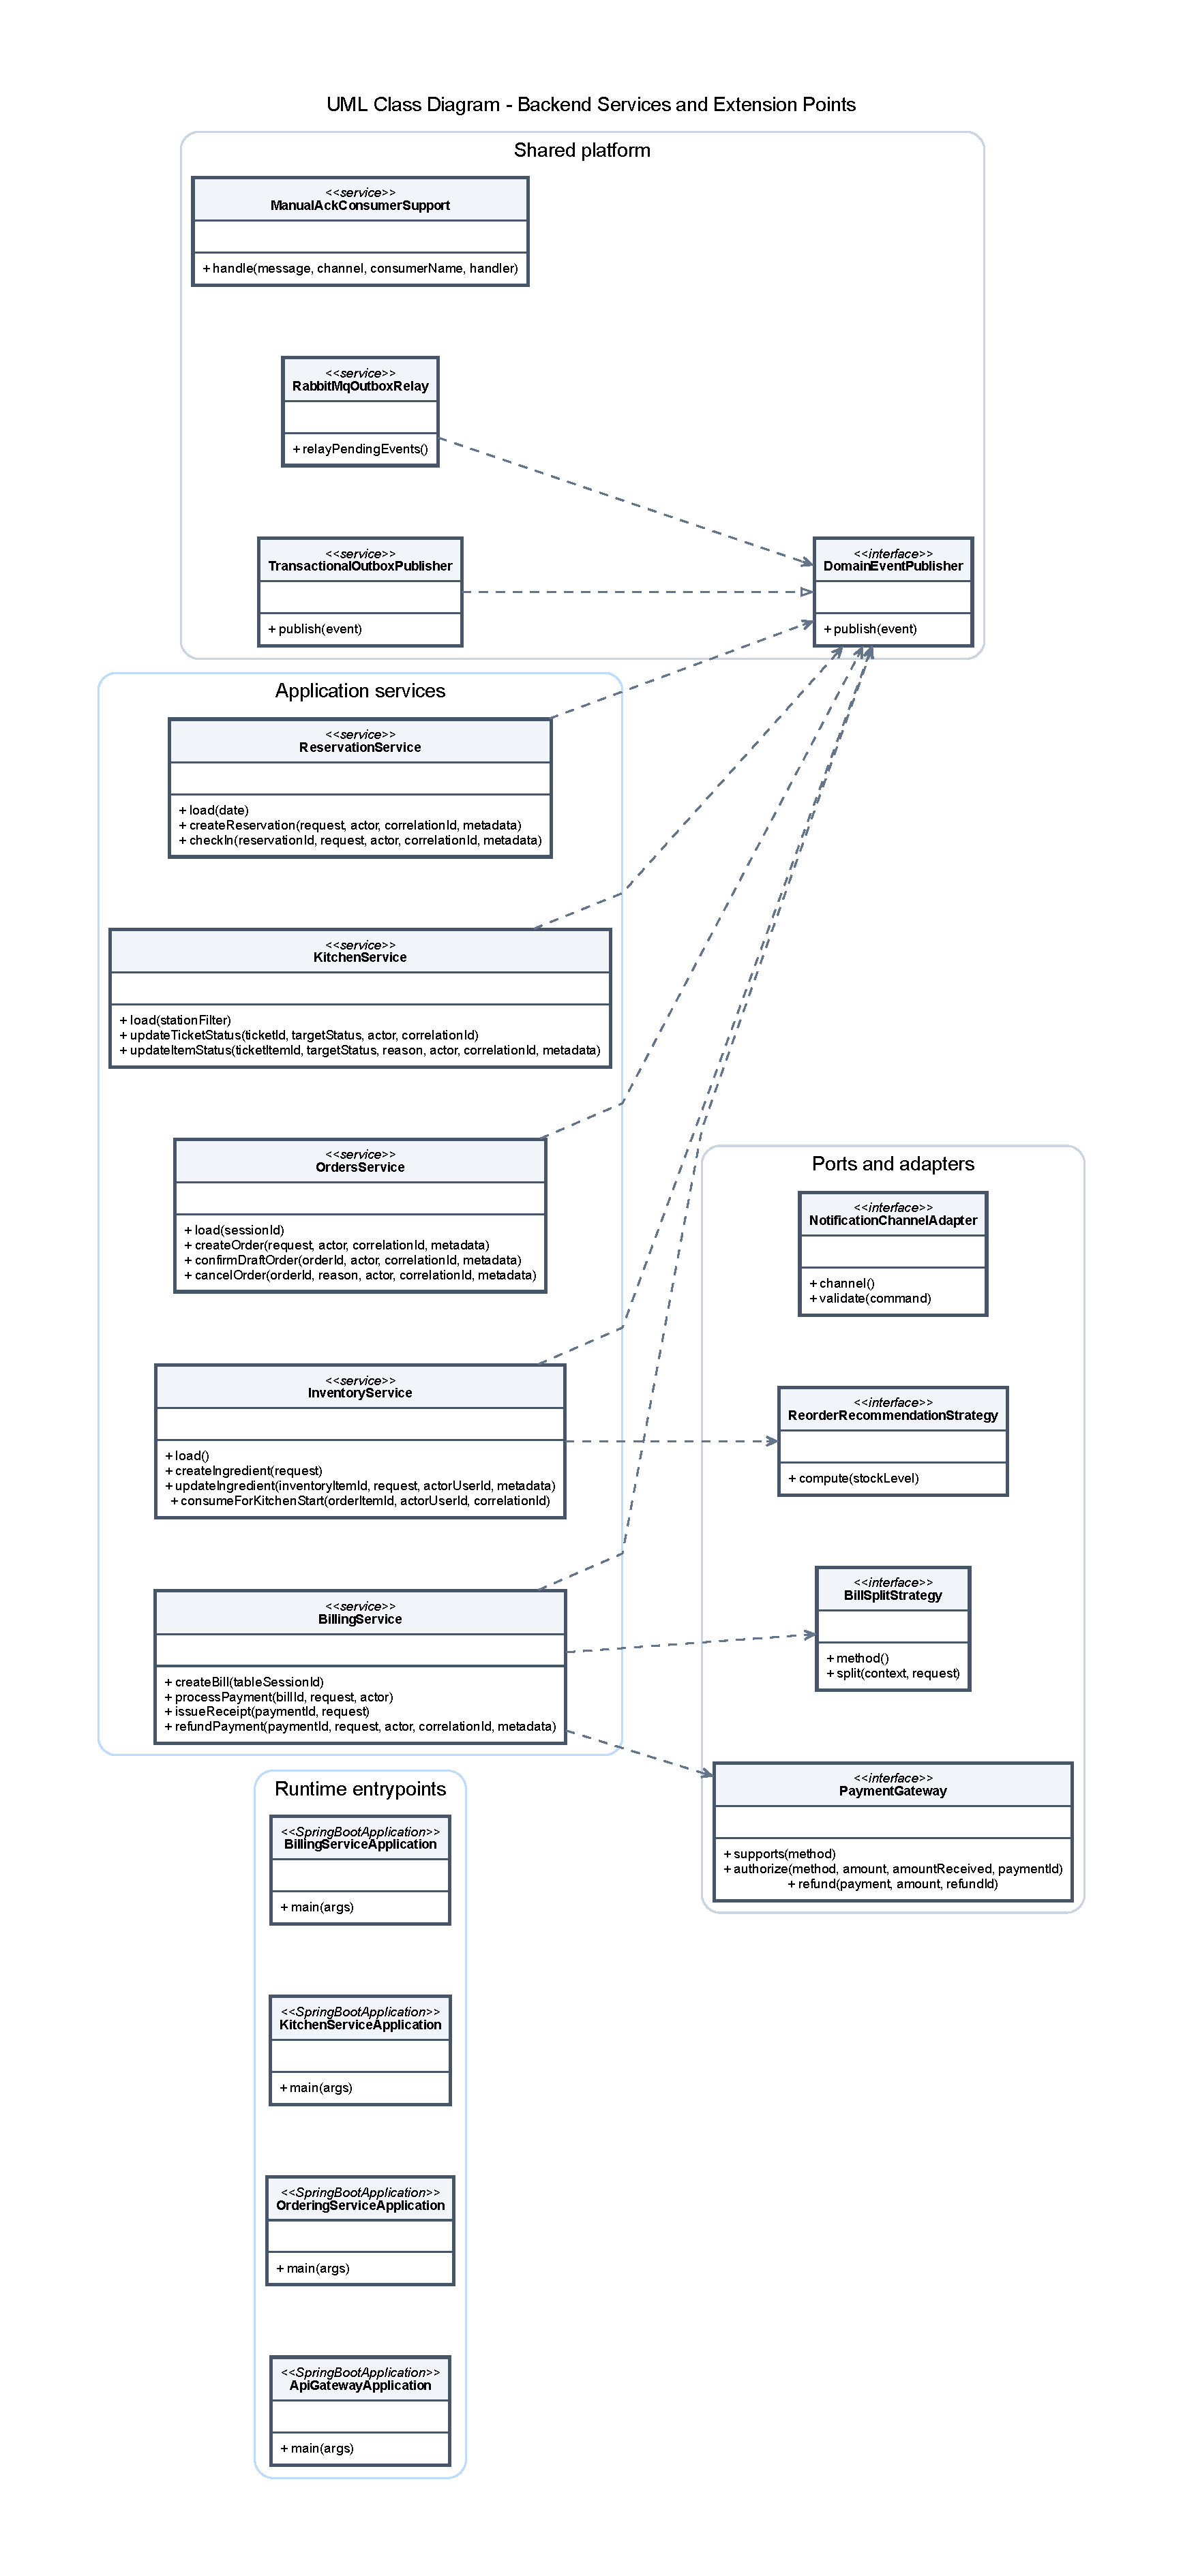
\includegraphics[width=0.97\linewidth,height=0.84\textheight,keepaspectratio]{18_uml_class_diagram_core_domain_overview.pdf}
}{
  \IfFileExists{18_uml_class_diagram_core_domain_overview.png}{
    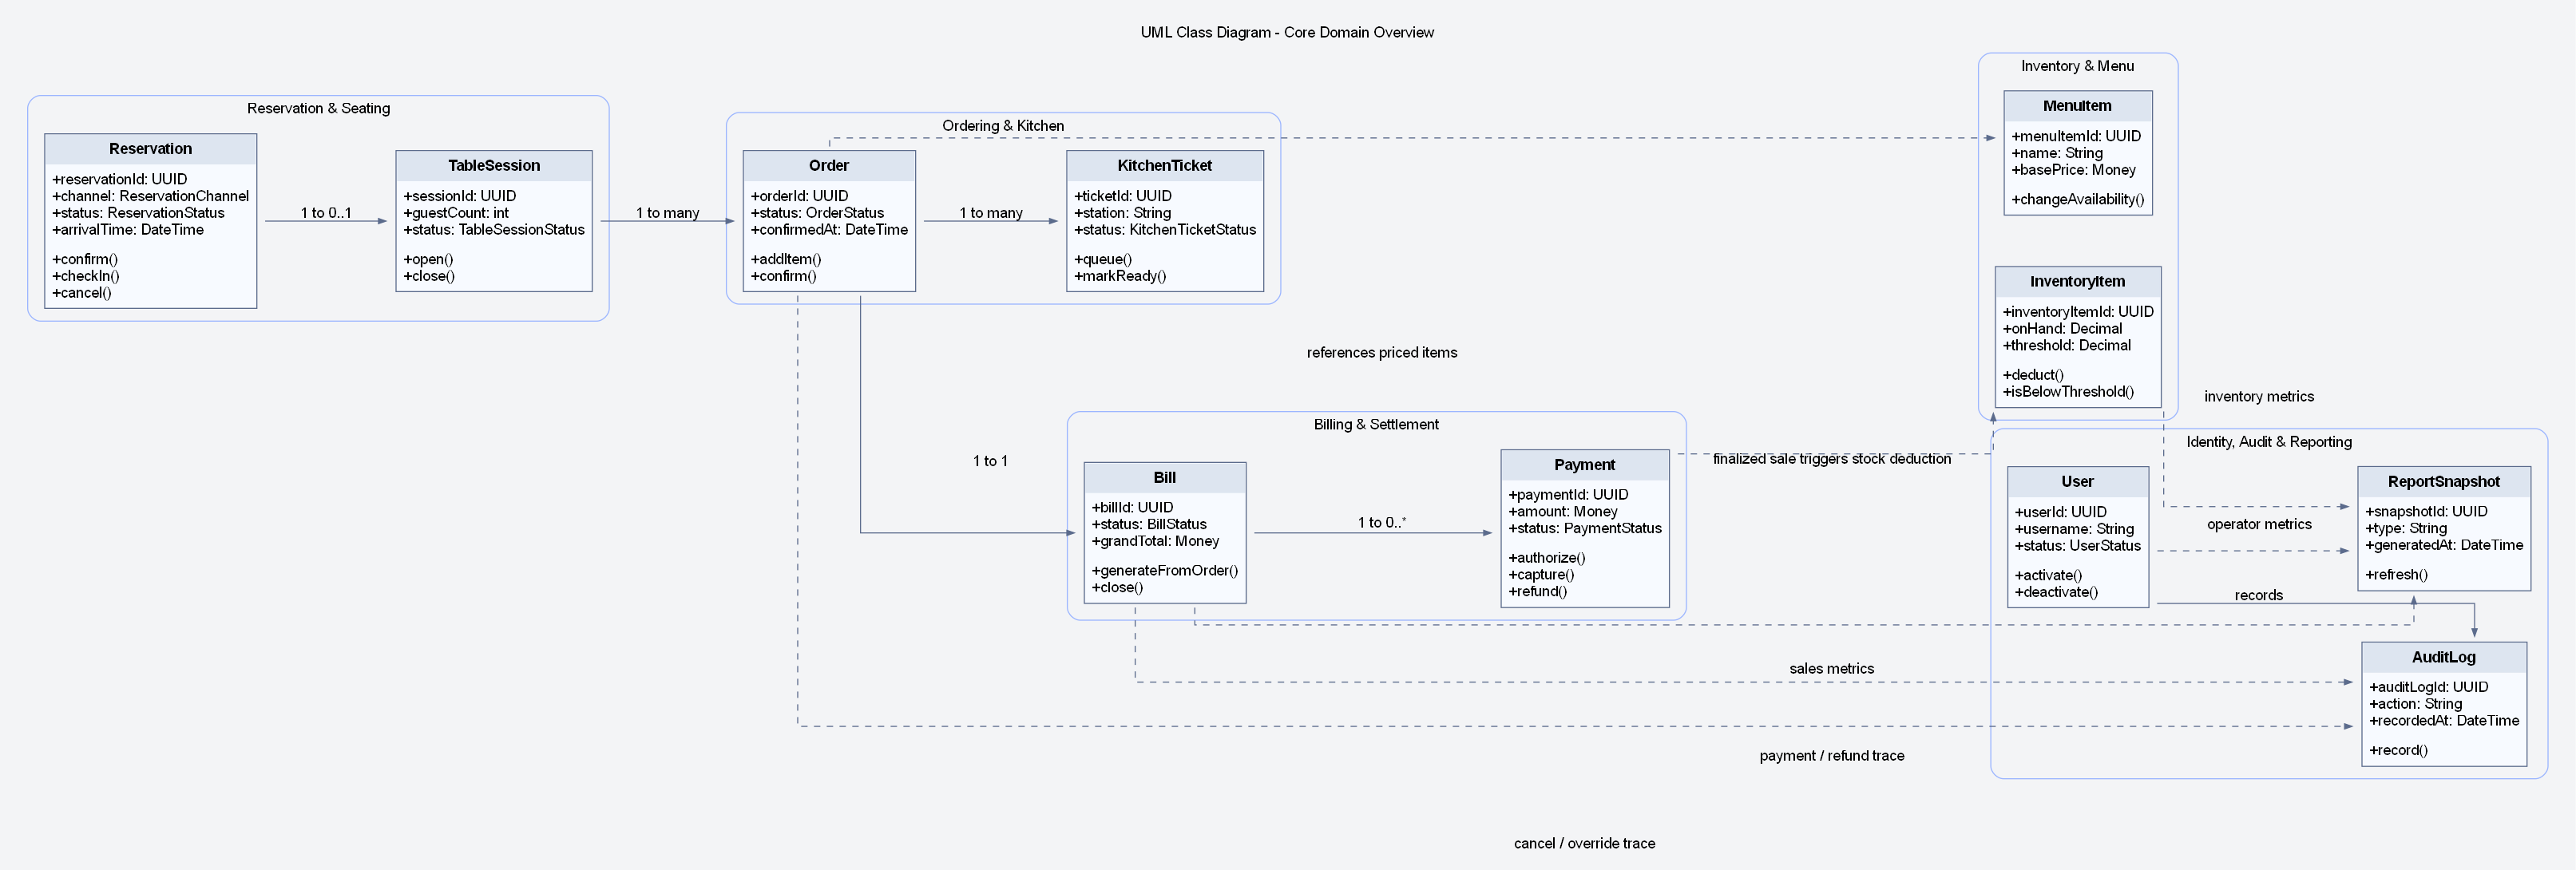
\includegraphics[width=0.97\linewidth,height=0.84\textheight,keepaspectratio]{18_uml_class_diagram_core_domain_overview.png}
  }{
    \fbox{\parbox{0.82\linewidth}{Thiếu file \textsf{18\_uml\_class\_diagram\_core\_domain\_overview.(pdf/png)}.}}
  }
}
\caption{Sơ đồ lớp tổng quan mô tả các service ứng dụng và các điểm mở rộng chính của backend IRMS}
\label{fig:irms-class-core}
\end{figure}

Hình~\ref{fig:irms-class-core} đặt các class entrypoint và service chính cạnh các interface dùng chung, gồm \textsf{DomainEventPublisher}, \textsf{PaymentGateway}, \textsf{BillSplitStrategy}, \textsf{ReorderRecommendationStrategy} và \textsf{NotificationChannelAdapter}. 

\begin{figure}[H]
\centering
\IfFileExists{19_uml_class_diagram_ordering_and_kitchen_cluster.pdf}{
  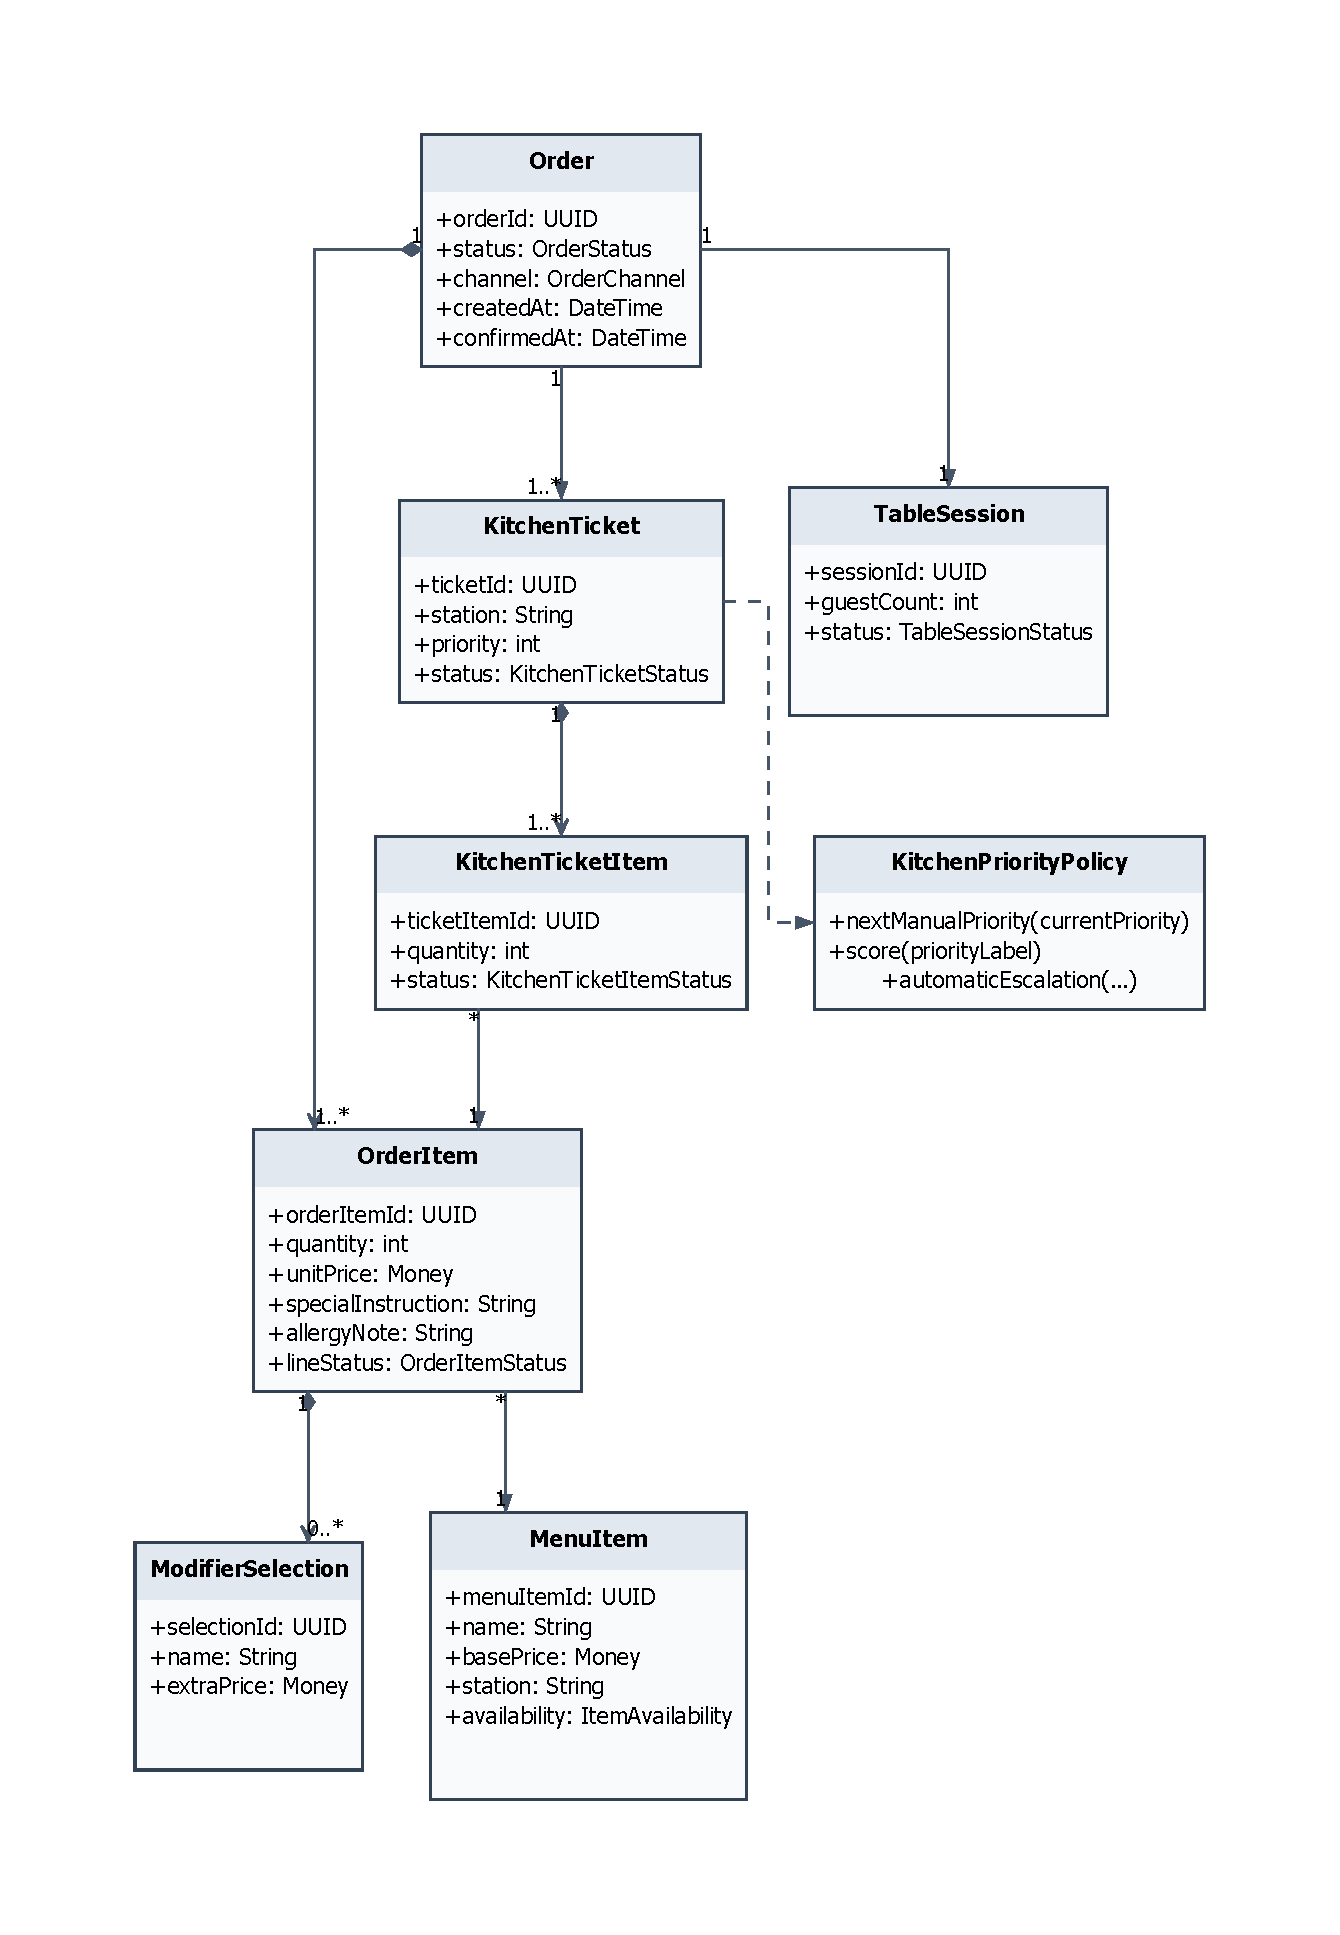
\includegraphics[width=0.97\linewidth,height=0.84\textheight,keepaspectratio]{19_uml_class_diagram_ordering_and_kitchen_cluster.pdf}
}{
  \IfFileExists{19_uml_class_diagram_ordering_and_kitchen_cluster.png}{
    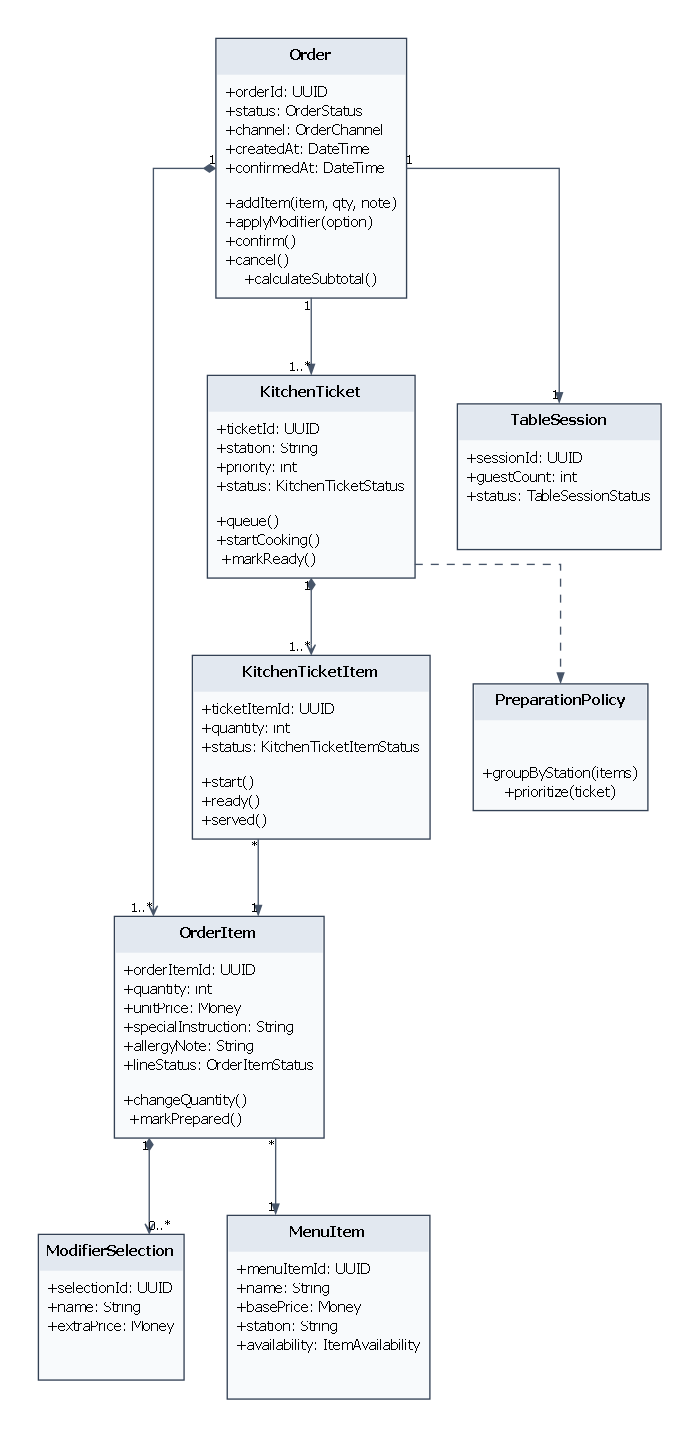
\includegraphics[width=0.97\linewidth,height=0.84\textheight,keepaspectratio]{19_uml_class_diagram_ordering_and_kitchen_cluster.png}
  }{
    \fbox{\parbox{0.82\linewidth}{Thiếu file \textsf{19\_uml\_class\_diagram\_ordering\_and\_kitchen\_cluster.(pdf/png)}.}}
  }
}
\caption{Sơ đồ lớp mô tả quan hệ giữa cụm \textsf{ordering} và \textsf{kitchen}}
\label{fig:irms-class-ordering-kitchen}
\end{figure}

Hình~\ref{fig:irms-class-ordering-kitchen} mô tả quan hệ giữa \textsf{OrdersController}, \textsf{OrdersService}, các service con của module \texttt{ordering}, cổng \textsf{KitchenCoordinationPort}, adapter \textsf{RemoteKitchenOrderRoutingClient} và phía nhận ở module \texttt{kitchen}. Quan hệ này khớp với C\&C View: module gọi món không truy cập thẳng persistence của bếp mà đi qua client tích hợp và controller nội bộ.

\begin{figure}[H]
\centering
\IfFileExists{20_uml_class_diagram_billing_inventory_and_governance_cluster.pdf}{
  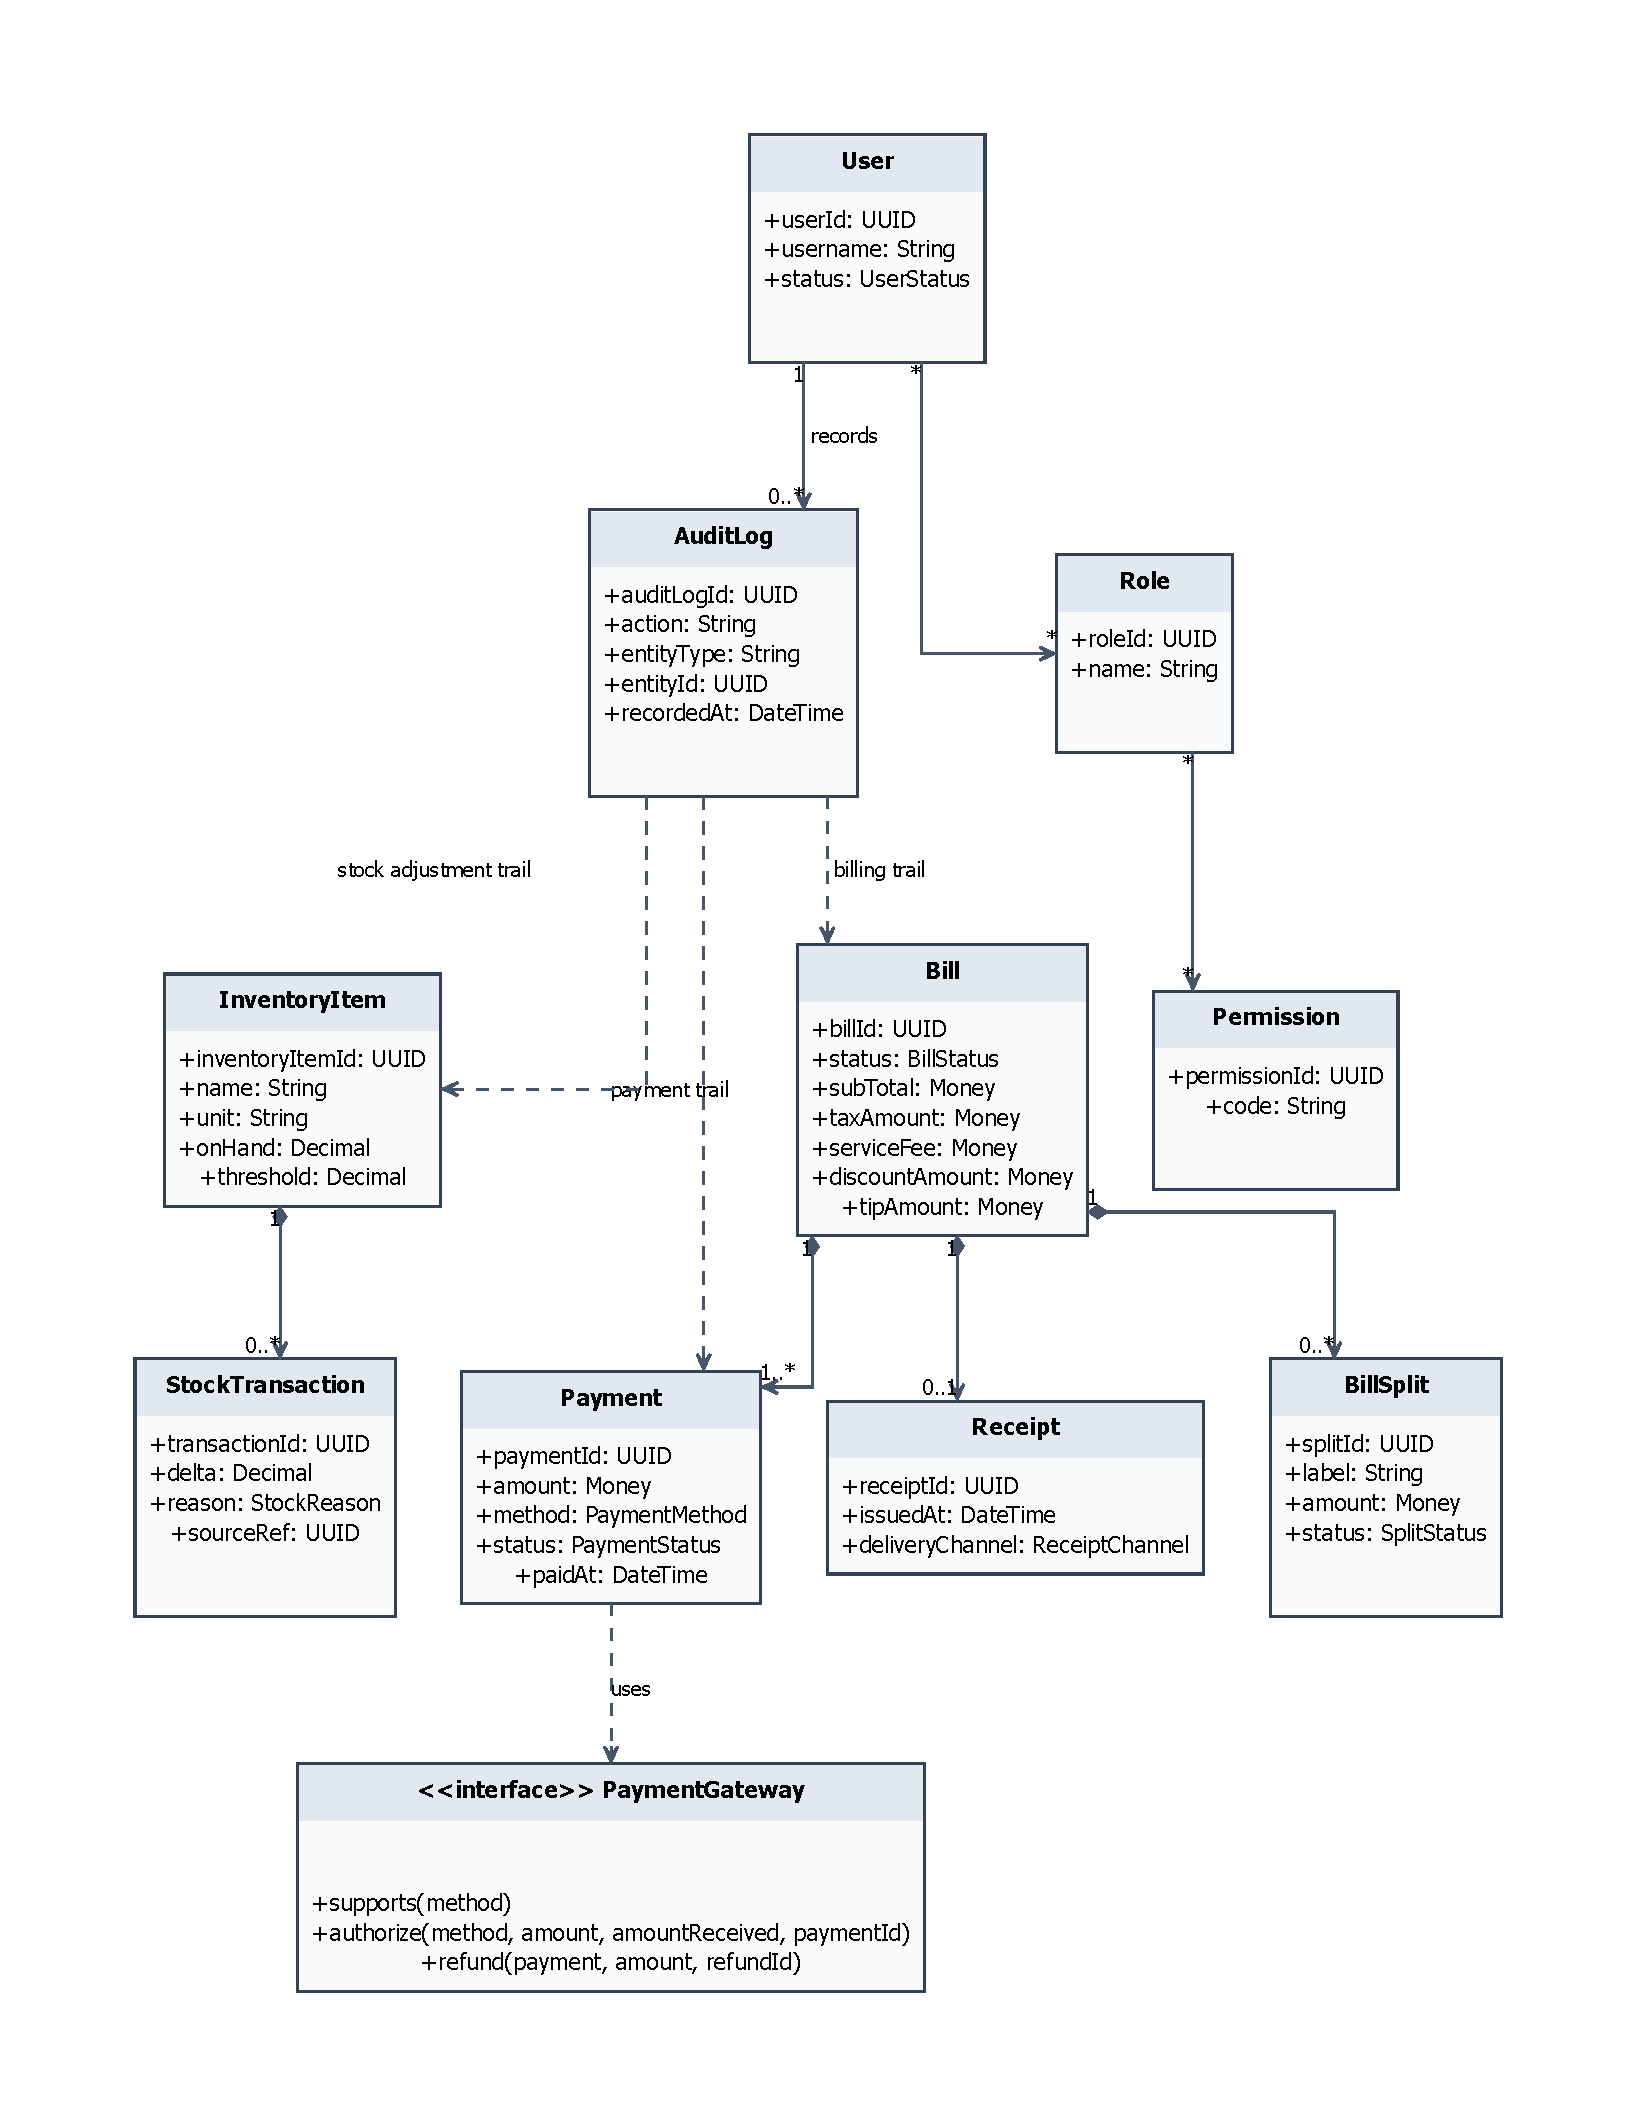
\includegraphics[width=0.97\linewidth,height=0.84\textheight,keepaspectratio]{20_uml_class_diagram_billing_inventory_and_governance_cluster.pdf}
}{
  \IfFileExists{20_uml_class_diagram_billing_inventory_and_governance_cluster.png}{
    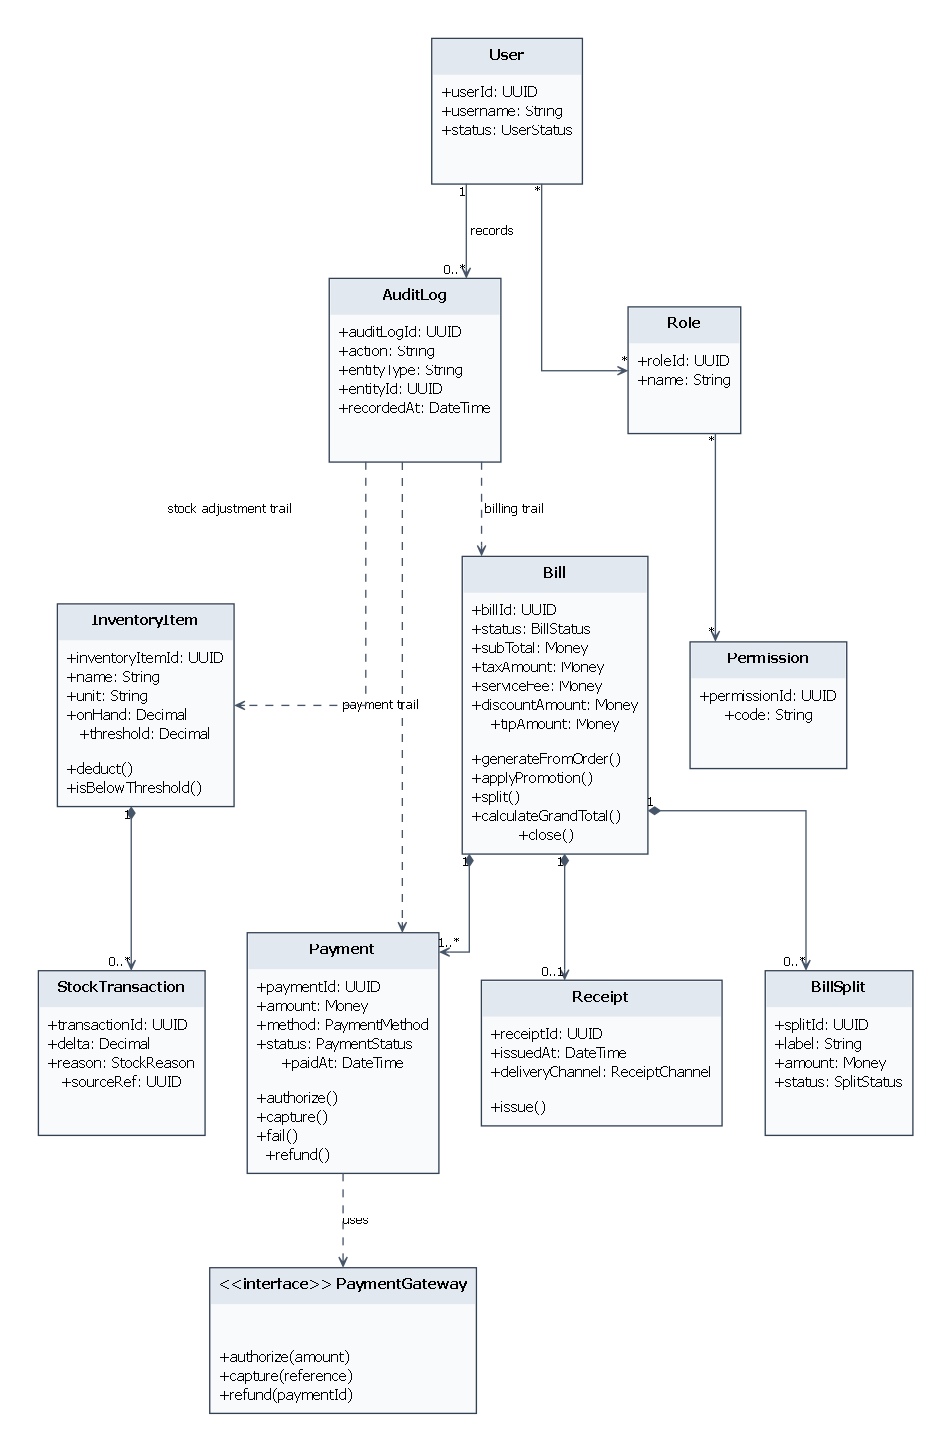
\includegraphics[width=0.97\linewidth,height=0.84\textheight,keepaspectratio]{20_uml_class_diagram_billing_inventory_and_governance_cluster.png}
  }{
    \fbox{\parbox{0.82\linewidth}{Thiếu file \textsf{20\_uml\_class\_diagram\_billing\_inventory\_and\_governance\_cluster.(pdf/png)}.}}
  }
}
\caption{Sơ đồ lớp mô tả các điểm mở rộng của cụm \textsf{billing}, \textsf{inventory} và governance}
\label{fig:irms-class-billing-inventory}
\end{figure}

Hình~\ref{fig:irms-class-billing-inventory} gom các điểm mở rộng nhạy cảm của hệ thống. Phần billing có \textsf{PaymentGateway} và các adapter thanh toán. Phần inventory có \textsf{LowStockSeverityPolicy} và \textsf{UsageBasedReorderRecommendationStrategy}. Vùng kiểm soát có \textsf{AuthService}, \textsf{AuditService}, \textsf{AuditEventMaterializer} và \textsf{IdentityRepository}.

\subsection{Giải thích theo từng cụm lớp}\label{sec:detailed-design-clusters}

\begin{figure}[H]
\centering
\IfFileExists{26_uml_class_diagram_reservation_and_seating_module.pdf}{
  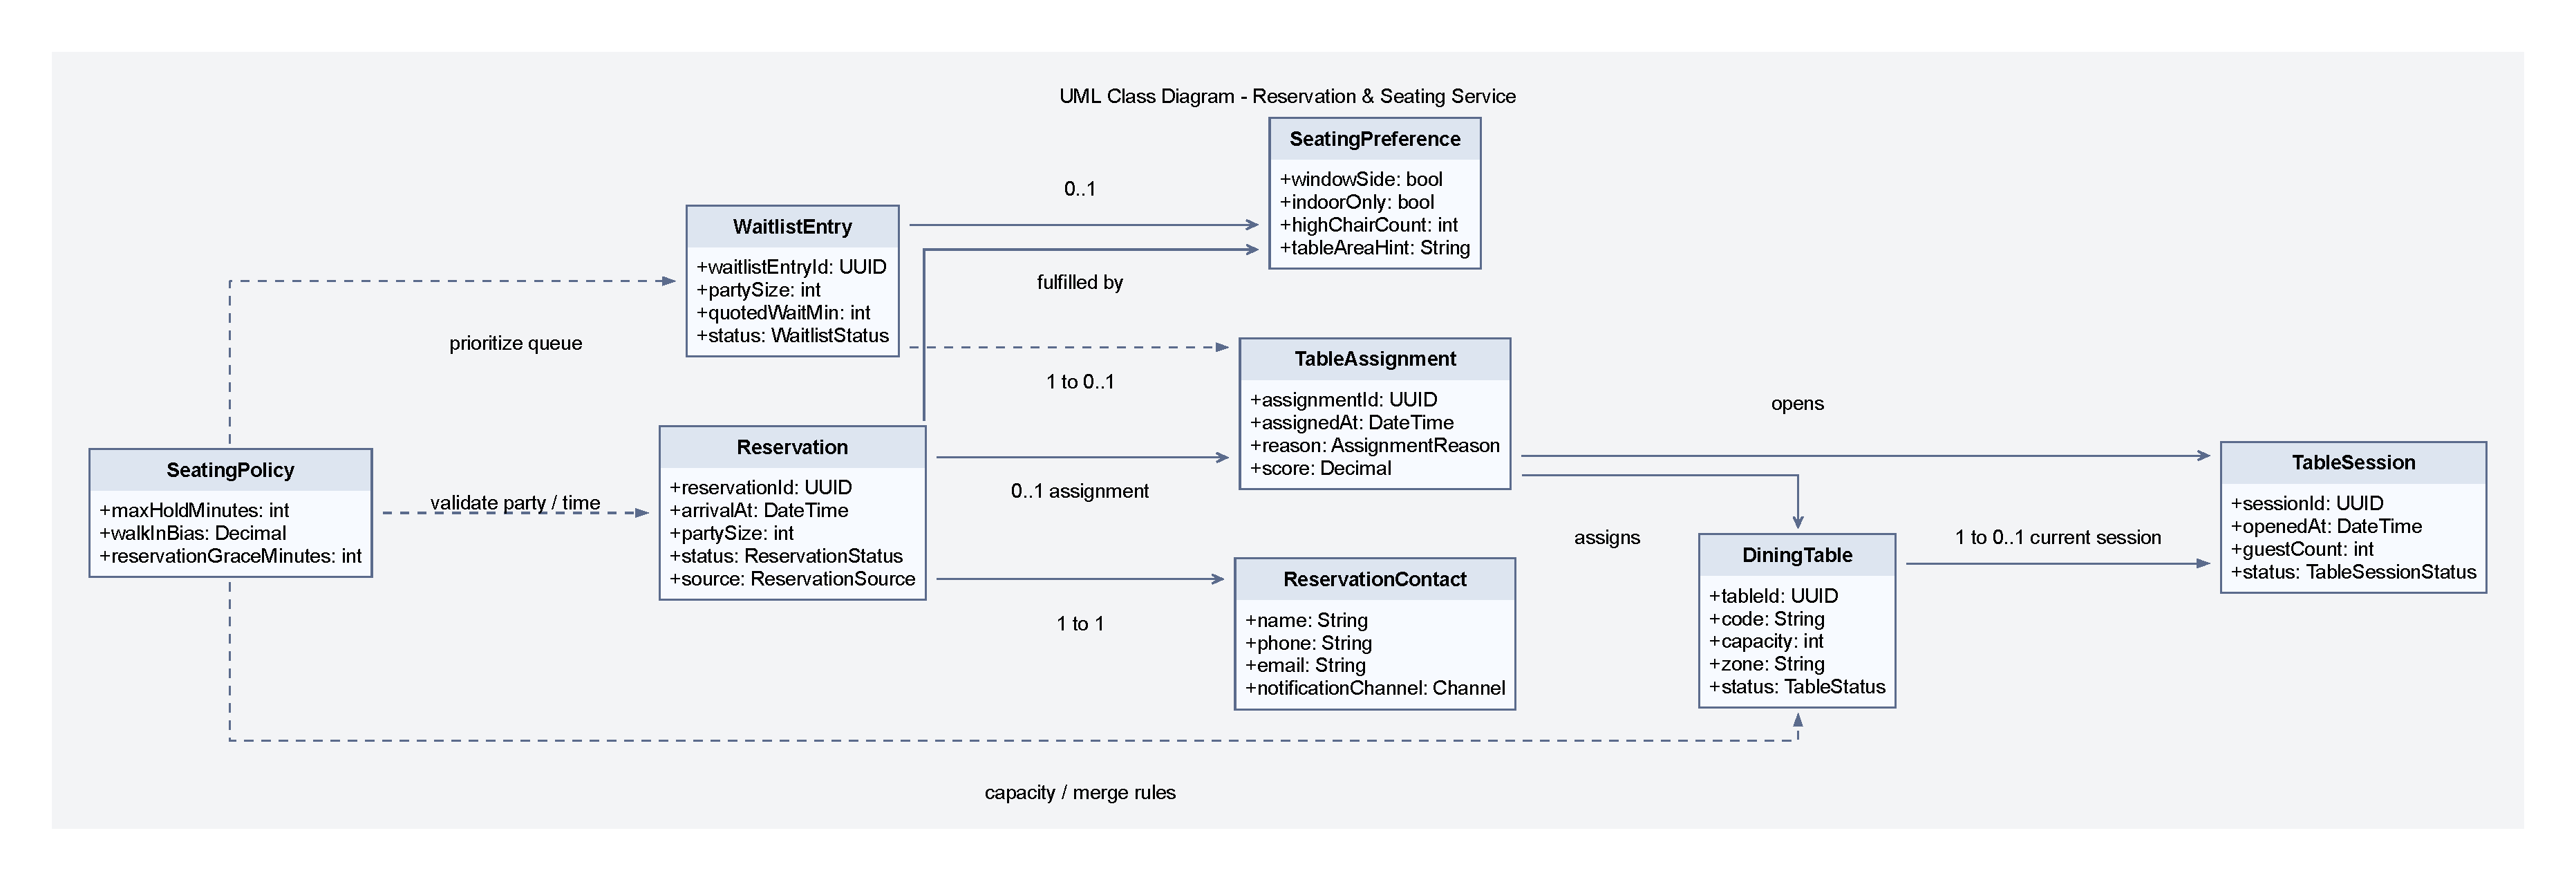
\includegraphics[width=0.97\linewidth,height=0.84\textheight,keepaspectratio]{26_uml_class_diagram_reservation_and_seating_module.pdf}
}{
  \IfFileExists{26_uml_class_diagram_reservation_and_seating_module.png}{
    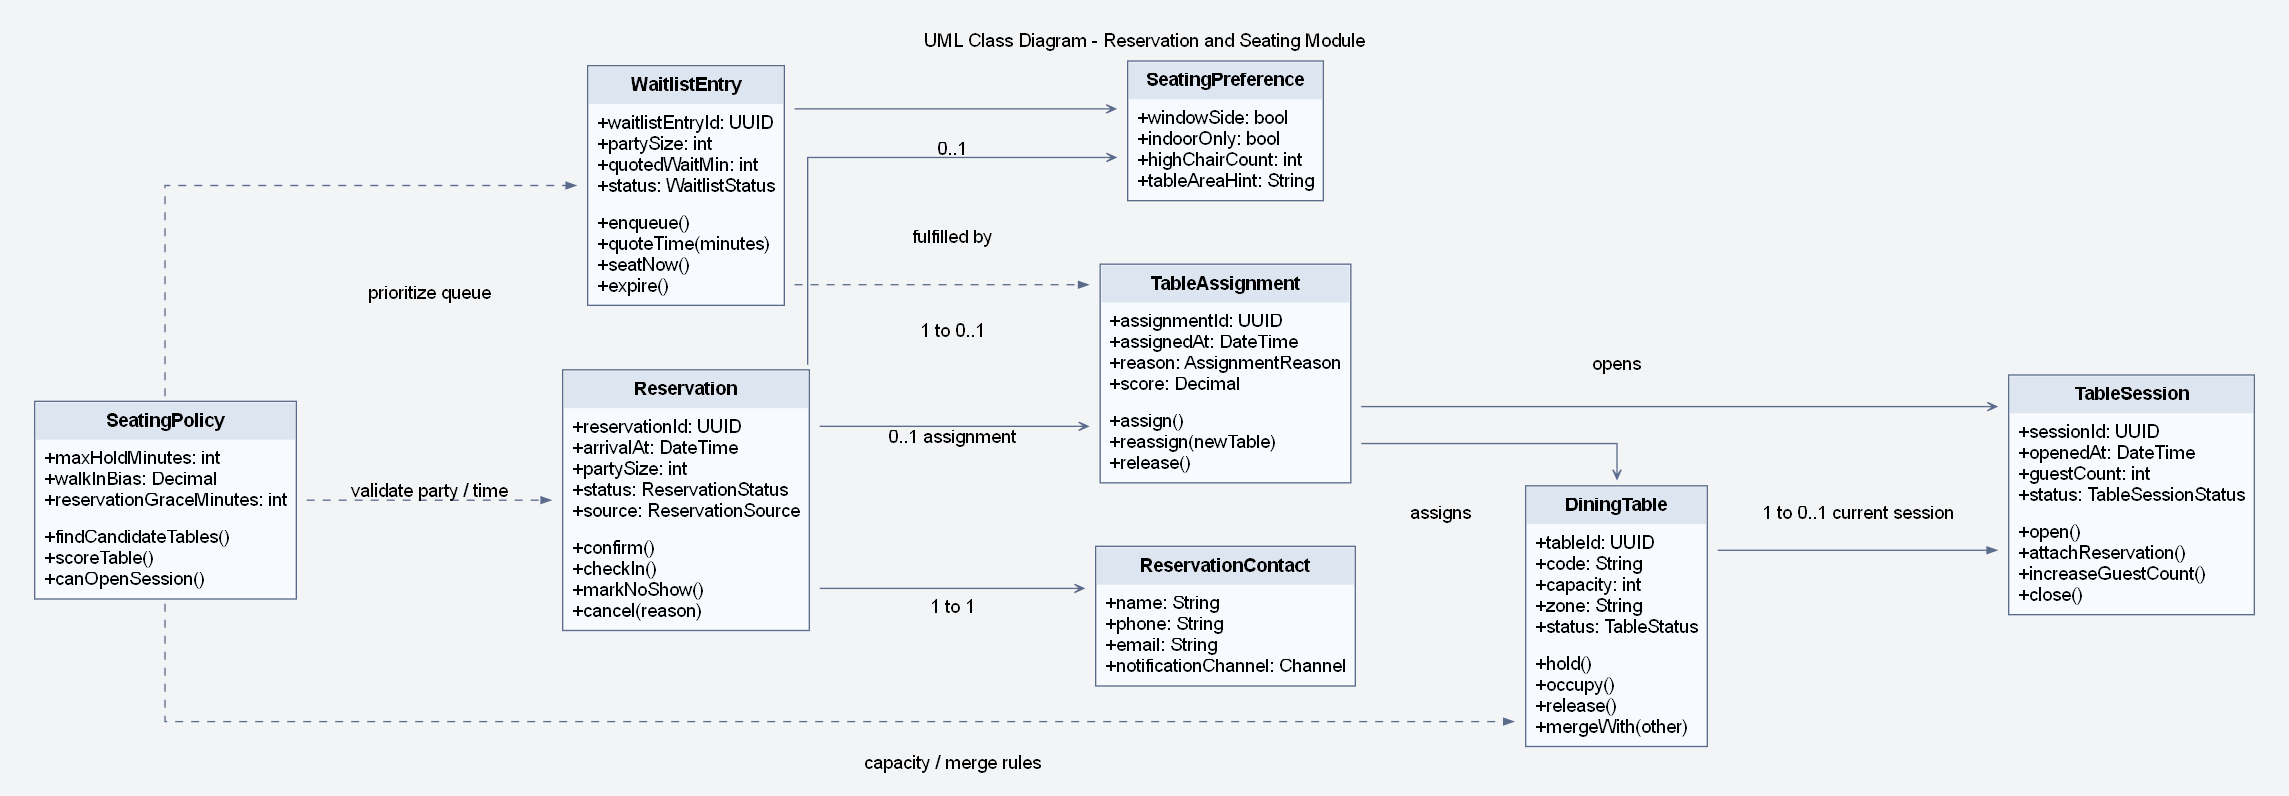
\includegraphics[width=0.97\linewidth,height=0.84\textheight,keepaspectratio]{26_uml_class_diagram_reservation_and_seating_module.png}
  }{
    \fbox{\parbox{0.82\linewidth}{Thiếu file \textsf{26\_uml\_class\_diagram\_reservation\_and\_seating\_module.(pdf/png)}.}}
  }
}
\caption{Sơ đồ lớp chi tiết cho module \textsf{reservation}}
\label{fig:irms-class-reservation-module}
\end{figure}

Hình~\ref{fig:irms-class-reservation-module} thể hiện các controller \textsf{ReservationController}, \textsf{TableController}, \textsf{WaitlistController}; service \textsf{ReservationService}, \textsf{ReservationCheckInService}, \textsf{ReservationWaitlistService}; workflow \textsf{ReservationSeatingMediator}; và các port/adapter JDBC cho vòng đời đặt bàn và bàn ăn. Các method trong hình được lấy từ class thật, ví dụ \textsf{load}, \textsf{recommend}, \textsf{createReservation} và \textsf{checkIn}.

\begin{figure}[H]
\centering
\IfFileExists{27_uml_class_diagram_ordering_and_menu_module.pdf}{
  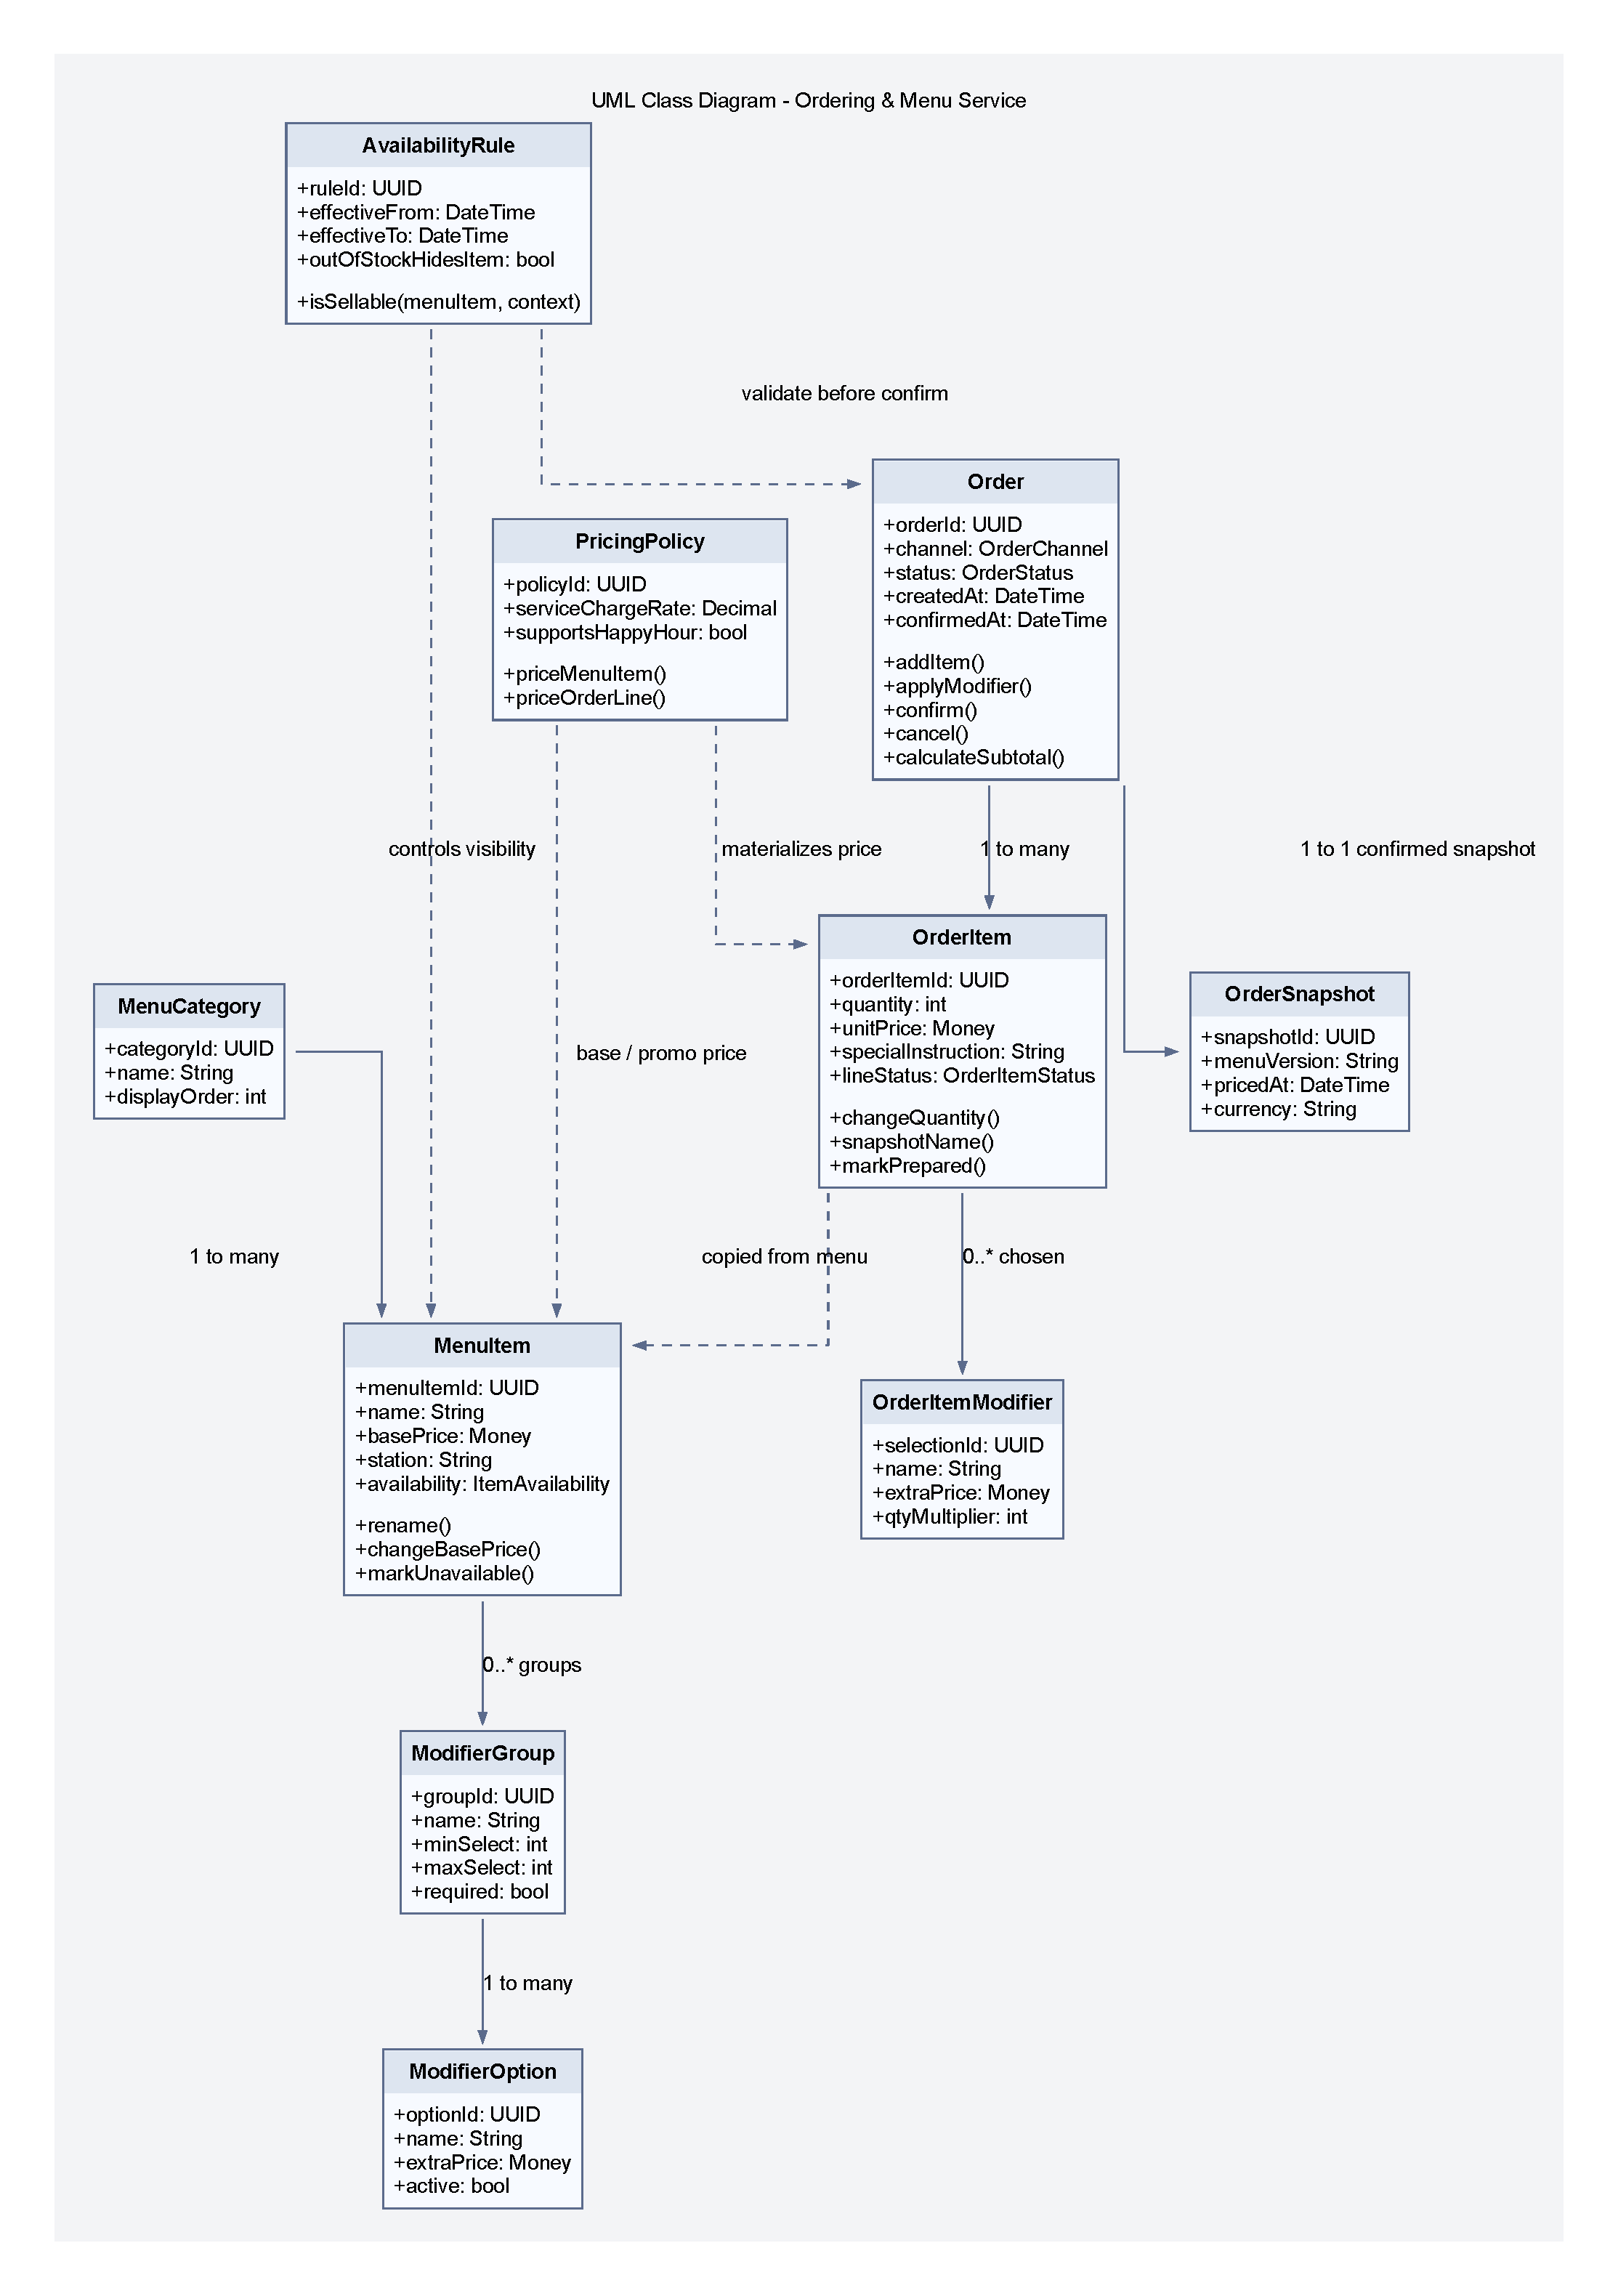
\includegraphics[width=0.97\linewidth,height=0.84\textheight,keepaspectratio]{27_uml_class_diagram_ordering_and_menu_module.pdf}
}{
  \IfFileExists{27_uml_class_diagram_ordering_and_menu_module.png}{
    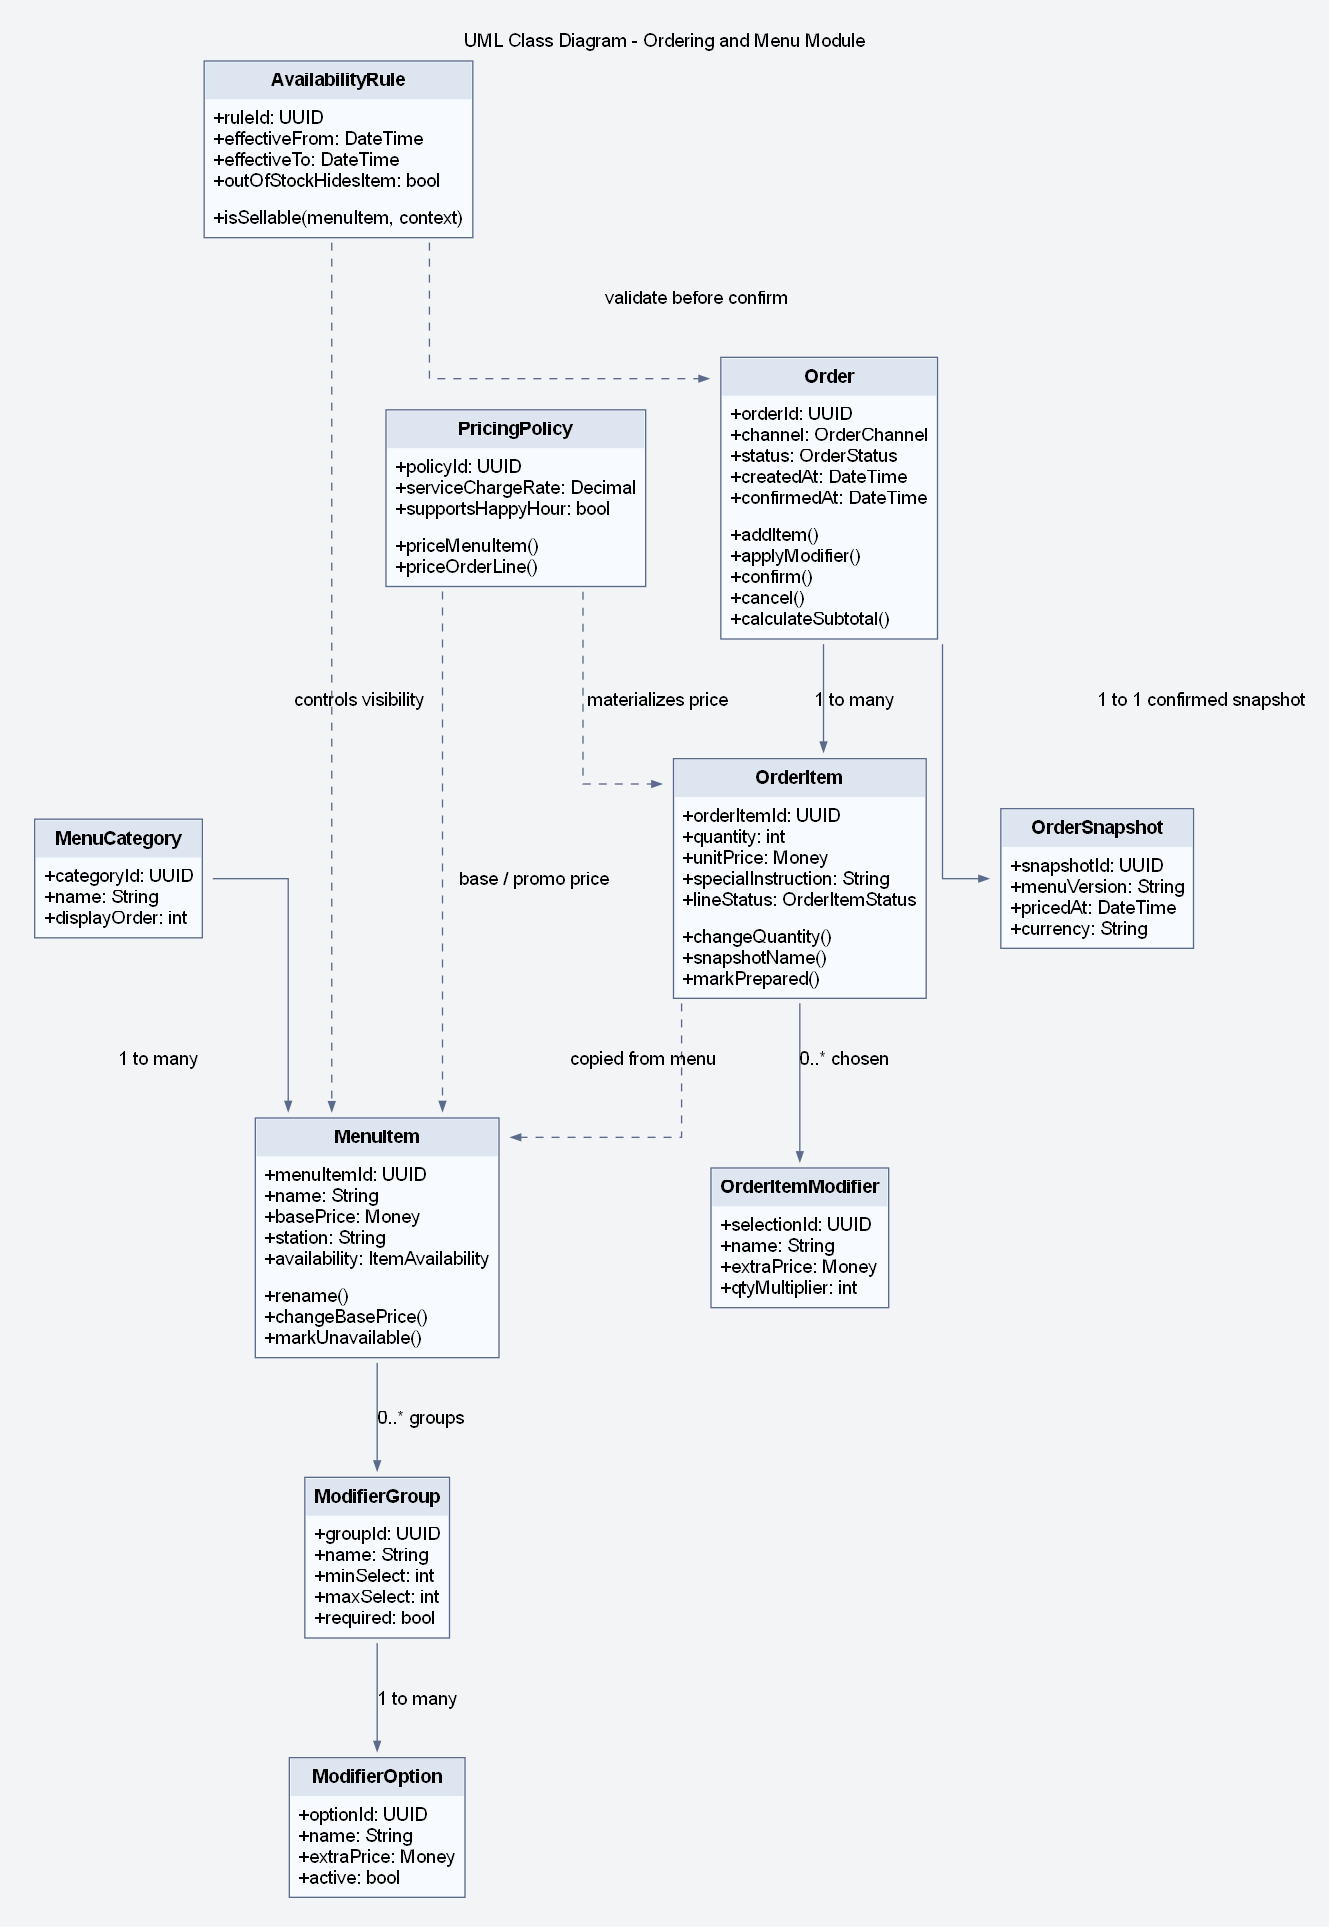
\includegraphics[width=0.97\linewidth,height=0.84\textheight,keepaspectratio]{27_uml_class_diagram_ordering_and_menu_module.png}
  }{
    \fbox{\parbox{0.82\linewidth}{Thiếu file \textsf{27\_uml\_class\_diagram\_ordering\_and\_menu\_module.(pdf/png)}.}}
  }
}
\caption{Sơ đồ lớp chi tiết cho module \textsf{ordering} và phần \textsf{menu}}
\label{fig:irms-class-ordering-module}
\end{figure}

Hình~\ref{fig:irms-class-ordering-module} làm rõ vai trò của \textsf{MenuItemController}, \textsf{OrdersController}, \textsf{MenuService}, \textsf{OrdersService}, \textsf{OrderCreationService}, \textsf{OrderMenuSelectionService}, các policy đơn hàng và hai phạm vi triển khaisitory port \textsf{OrderRepository}, \textsf{OrderQueryRepository}. Các adapter \textsf{JdbcOrderRepository} và \textsf{JdbcOrderQueryRepository} được đặt ở phía hiện thực port, đúng với nguyên tắc tách application service khỏi truy cập JDBC.

\begin{figure}[H]
\centering
\IfFileExists{28_uml_class_diagram_kitchen_coordination_module.pdf}{
  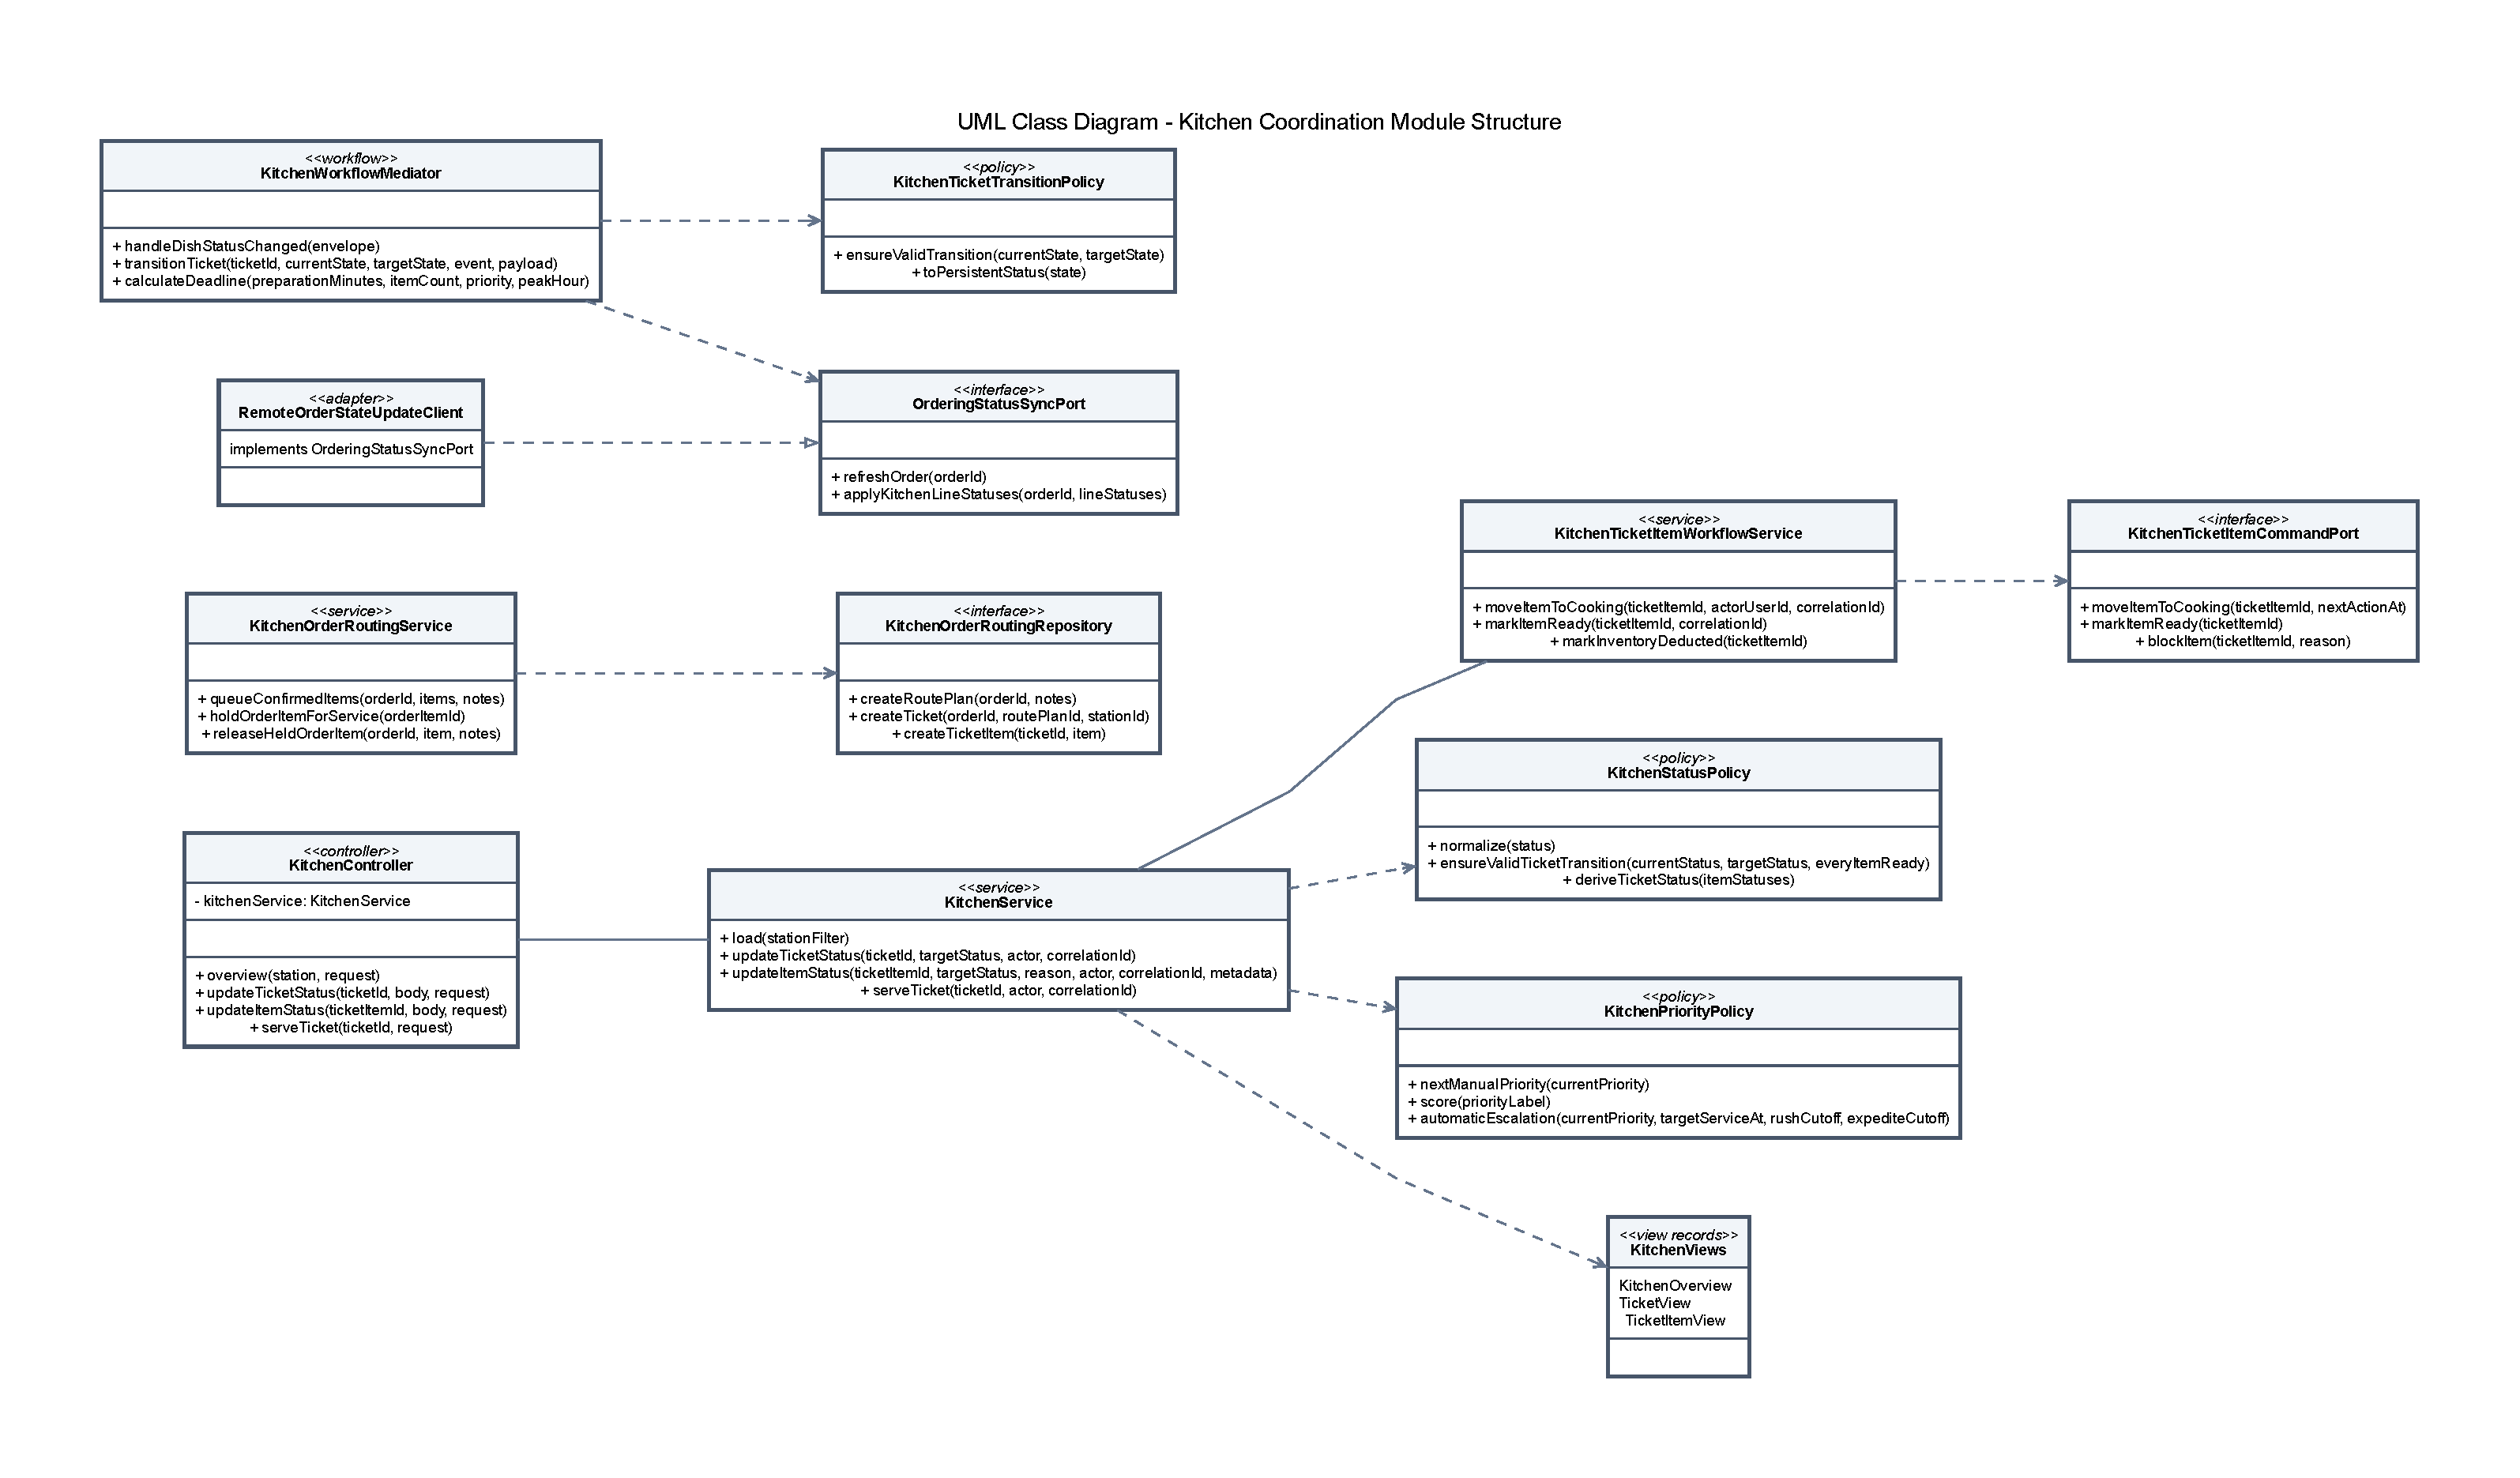
\includegraphics[width=0.97\linewidth,height=0.84\textheight,keepaspectratio]{28_uml_class_diagram_kitchen_coordination_module.pdf}
}{
  \IfFileExists{28_uml_class_diagram_kitchen_coordination_module.png}{
    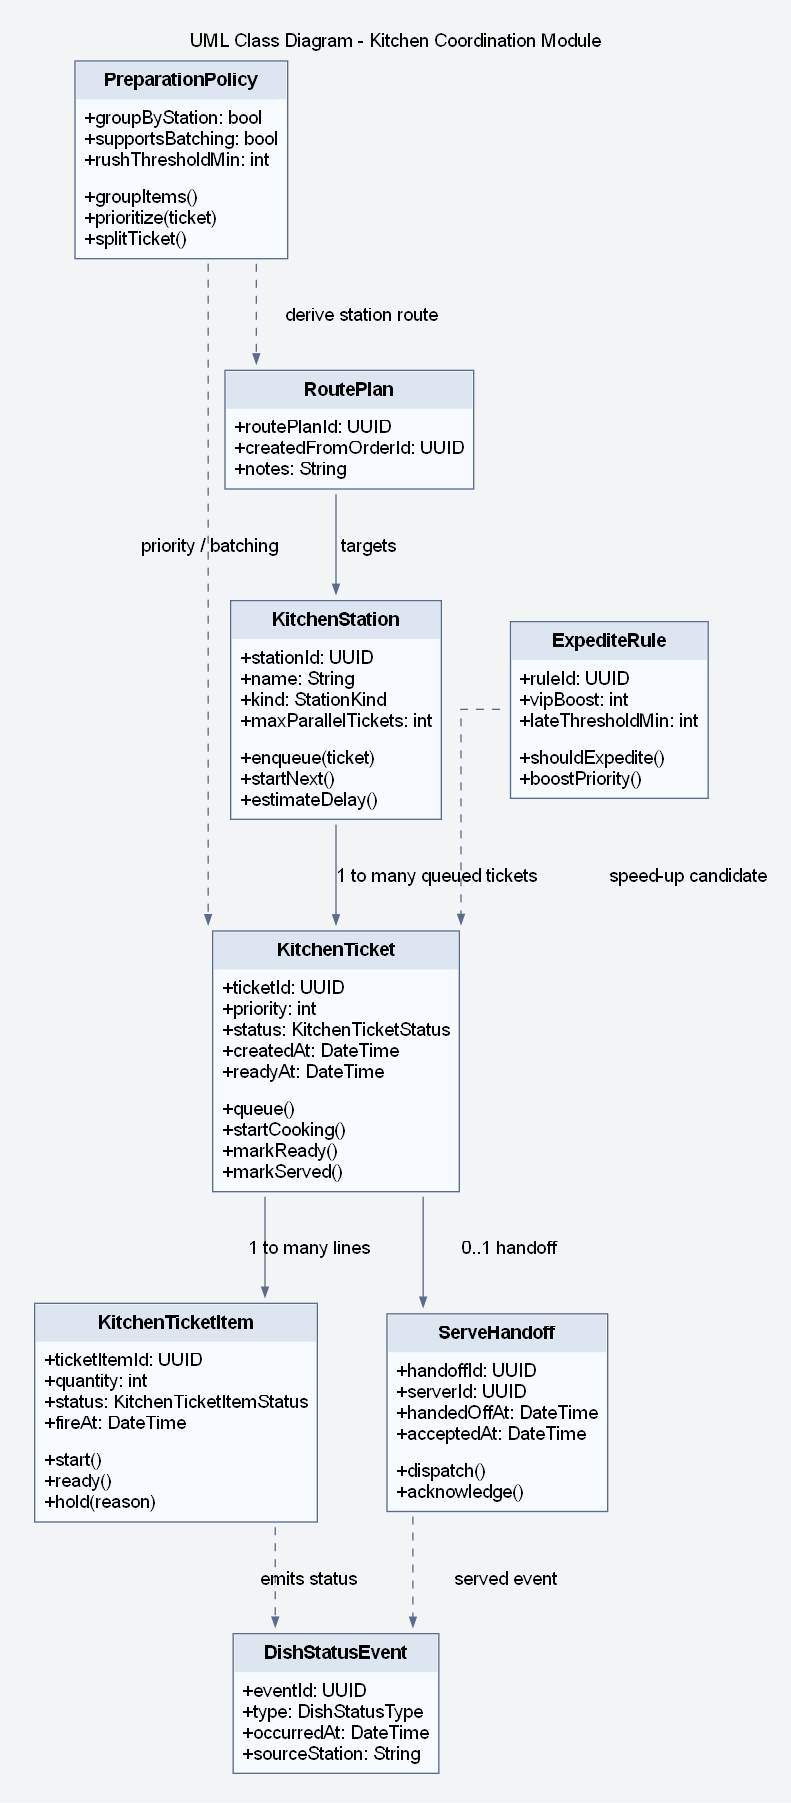
\includegraphics[width=0.97\linewidth,height=0.84\textheight,keepaspectratio]{28_uml_class_diagram_kitchen_coordination_module.png}
  }{
    \fbox{\parbox{0.82\linewidth}{Thiếu file \textsf{28\_uml\_class\_diagram\_kitchen\_coordination\_module.(pdf/png)}.}}
  }
}
\caption{Sơ đồ lớp chi tiết cho module \textsf{kitchen}}
\label{fig:irms-class-kitchen-module}
\end{figure}

Hình~\ref{fig:irms-class-kitchen-module} mô tả các lớp điều phối bếp thật như \textsf{KitchenService}, \textsf{KitchenOrderRoutingService}, \textsf{KitchenTicketItemWorkflowService}, \textsf{KitchenWorkflowMediator}, các policy trạng thái/ưu tiên và các port \textsf{KitchenOrderRoutingRepository}, \textsf{KitchenTicketItemCommandPort}, \textsf{OrderingStatusSyncPort}. Adapter \textsf{RemoteOrderStateUpdateClient} thể hiện phụ thuộc quay về trạng thái gọi món thông qua interface thay vì truy cập trực tiếp.

\begin{figure}[H]
\centering
\IfFileExists{29_uml_class_diagram_billing_and_settlement_module.pdf}{
  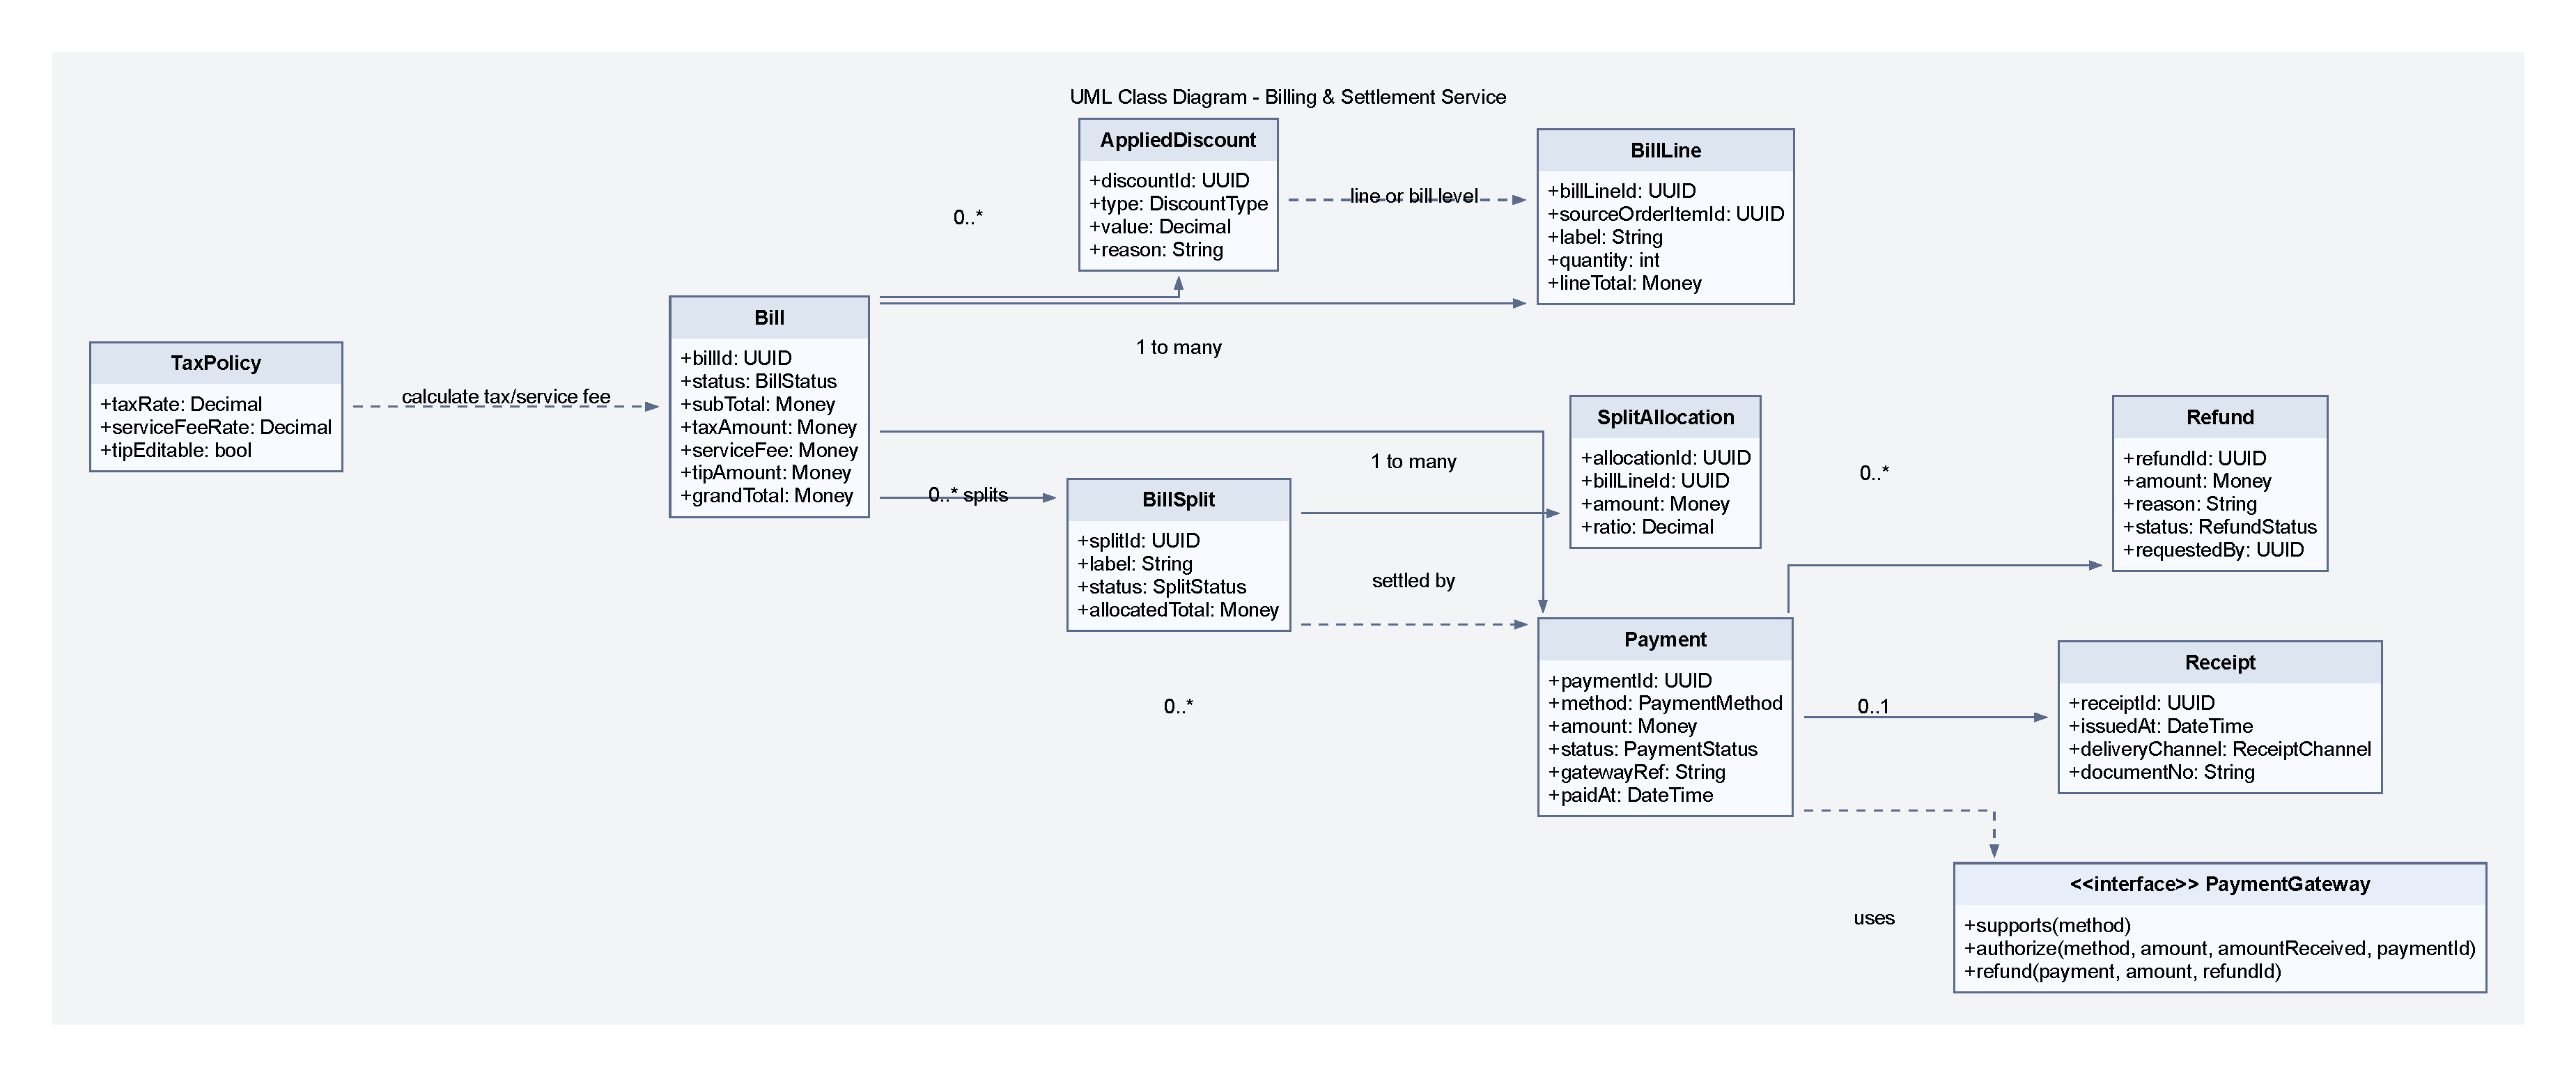
\includegraphics[width=0.97\linewidth,height=0.84\textheight,keepaspectratio]{29_uml_class_diagram_billing_and_settlement_module.pdf}
}{
  \IfFileExists{29_uml_class_diagram_billing_and_settlement_module.png}{
    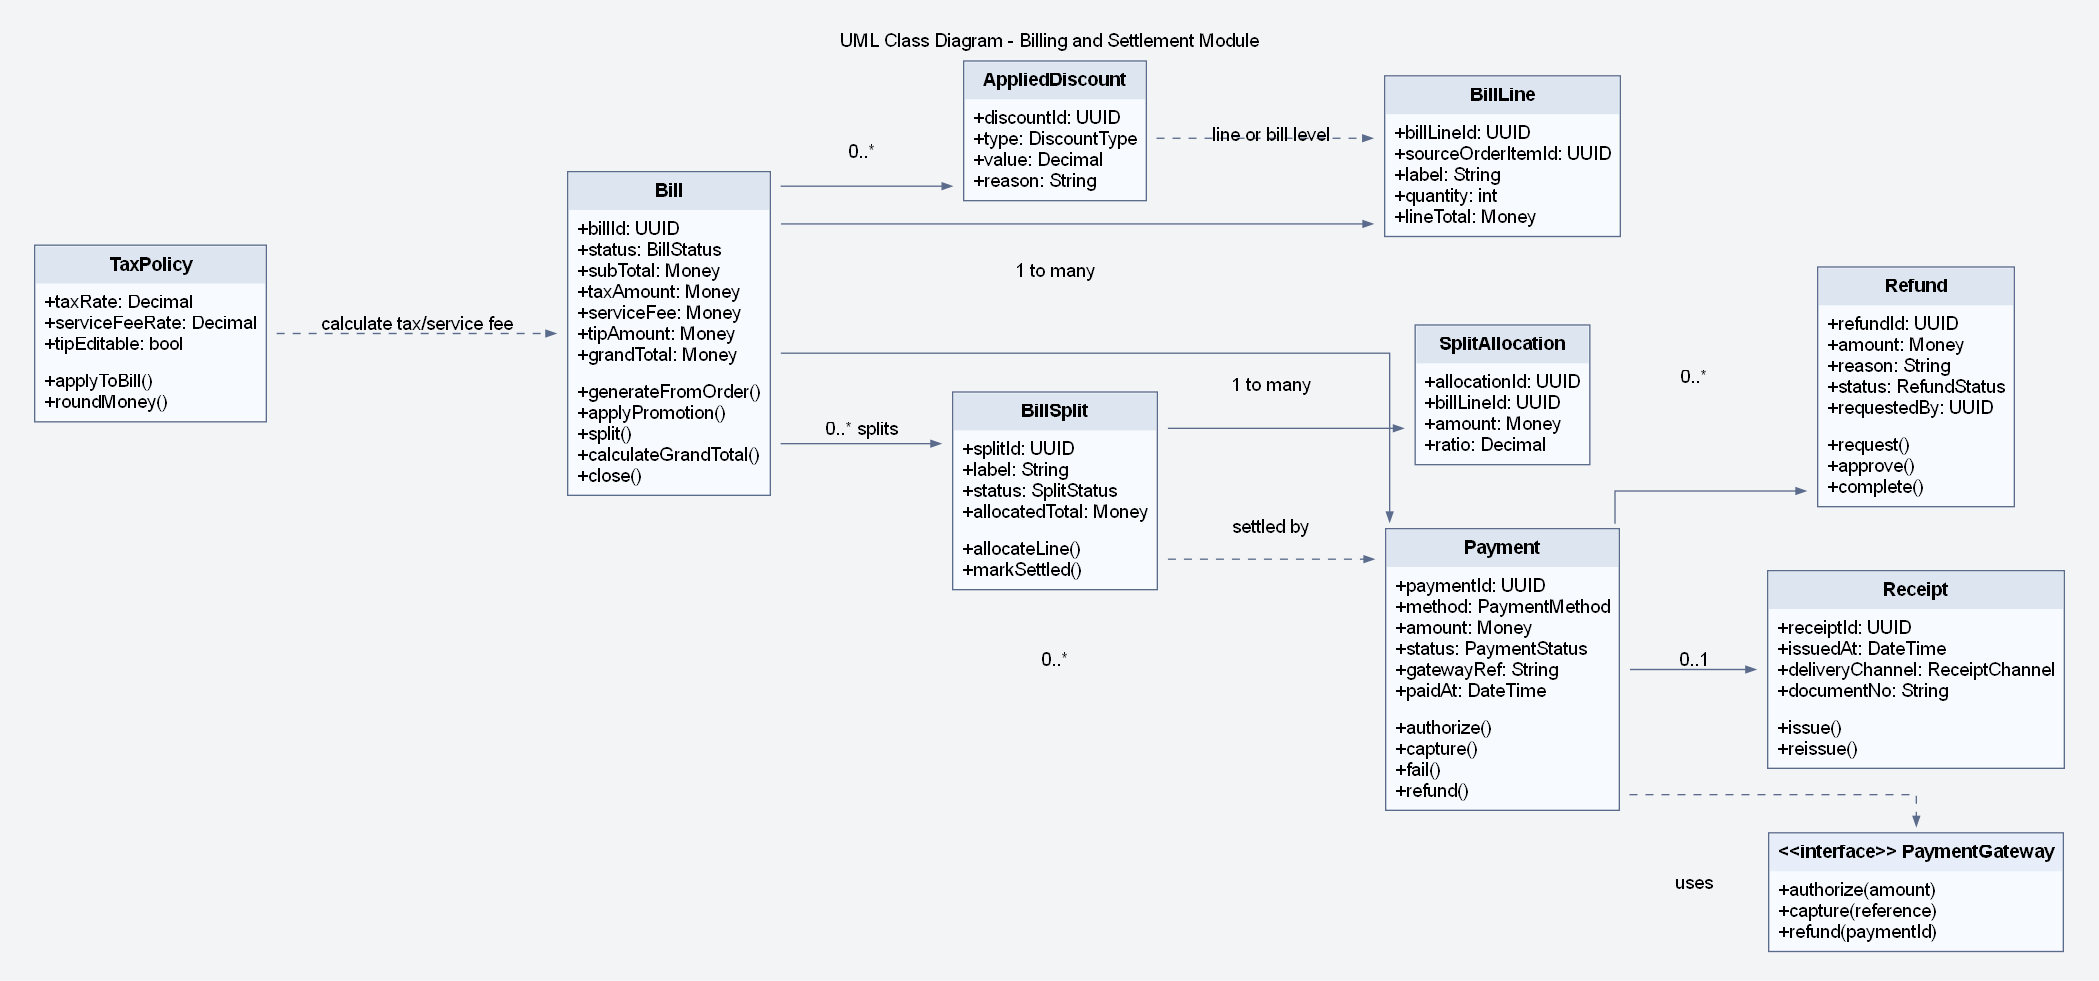
\includegraphics[width=0.97\linewidth,height=0.84\textheight,keepaspectratio]{29_uml_class_diagram_billing_and_settlement_module.png}
  }{
    \fbox{\parbox{0.82\linewidth}{Thiếu file \textsf{29\_uml\_class\_diagram\_billing\_and\_settlement\_module.(pdf/png)}.}}
  }
}
\caption{Sơ đồ lớp chi tiết cho module \textsf{billing}}
\label{fig:irms-class-billing-module}
\end{figure}

Hình~\ref{fig:irms-class-billing-module} thể hiện \textsf{BillingService} như facade ứng dụng. Các service con phụ trách lập hóa đơn, tách hóa đơn, thanh toán, biên nhận và hoàn tiền. Các điểm mở rộng chính là \textsf{BillSplitStrategy}, \textsf{PaymentGateway} và \textsf{ReceiptDeliveryAdapter}. Các strategy \textsf{EqualSplitStrategy}, \textsf{AmountSplitStrategy} và \textsf{SeatSplitStrategy} được biểu diễn bằng quan hệ hiện thực interface được dùng trong thiết kế.

\begin{figure}[H]
\centering
\IfFileExists{30_uml_class_diagram_inventory_and_notification_module.pdf}{
  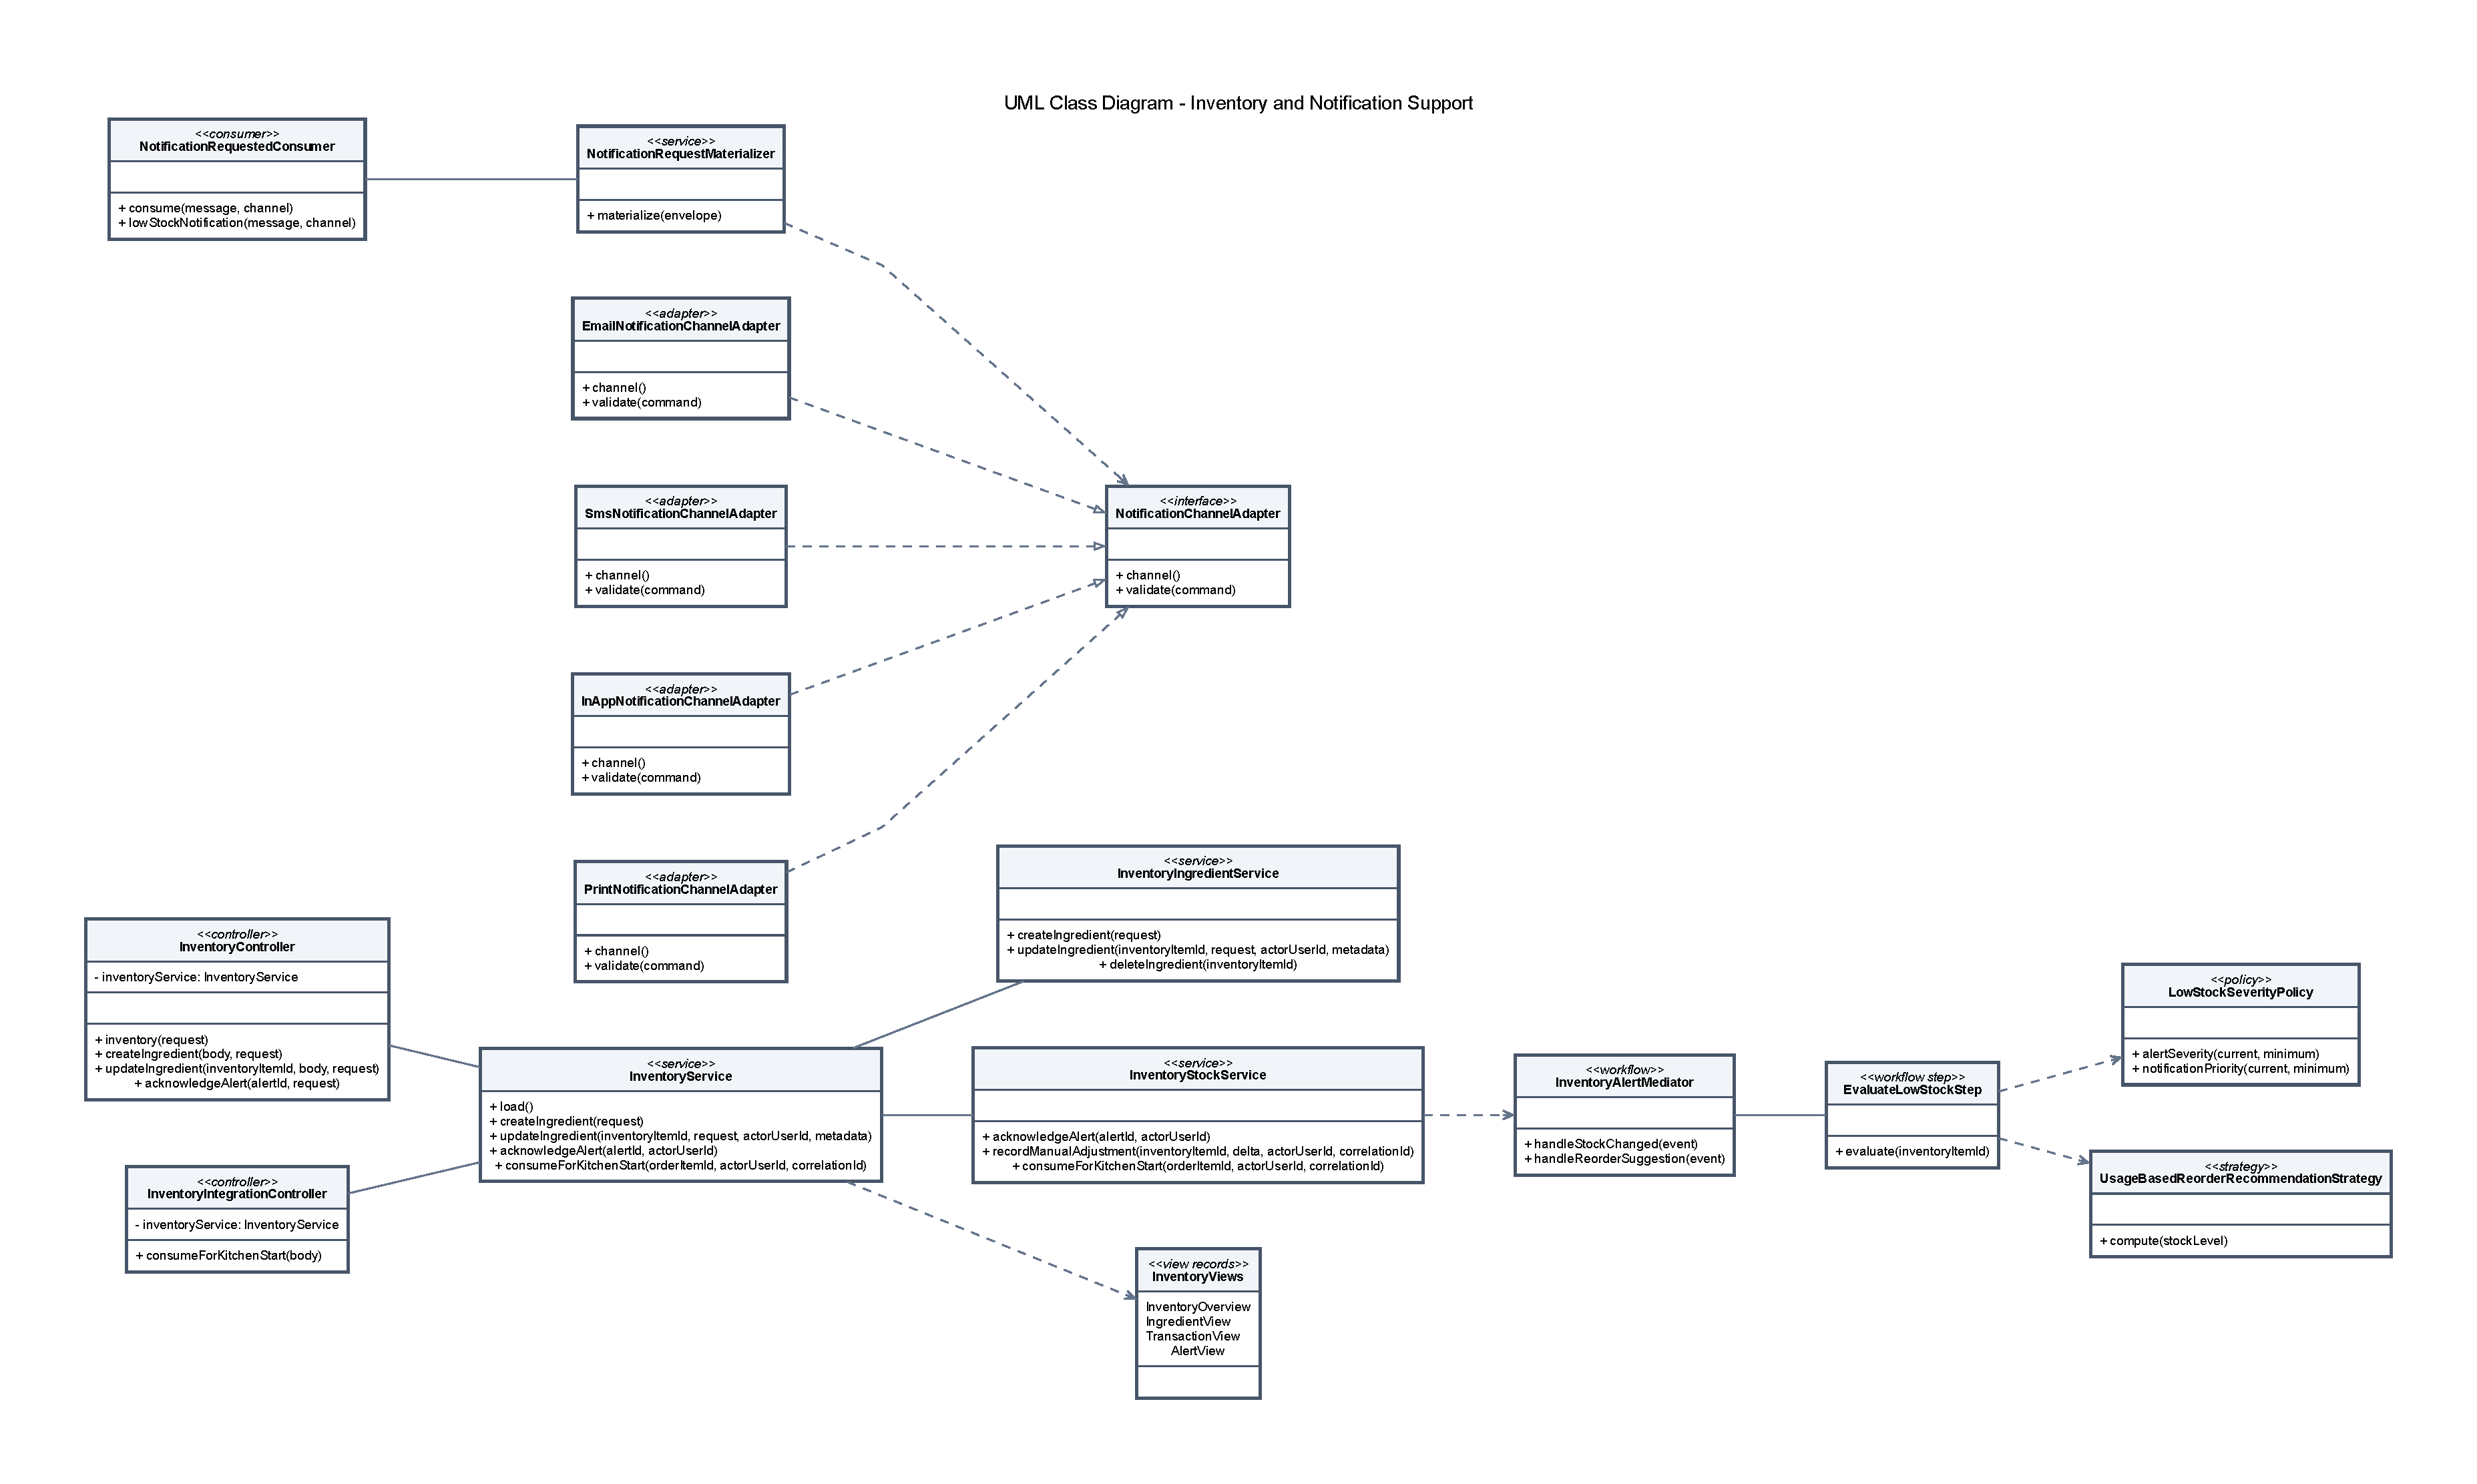
\includegraphics[width=0.97\linewidth,height=0.84\textheight,keepaspectratio]{30_uml_class_diagram_inventory_and_notification_module.pdf}
}{
  \IfFileExists{30_uml_class_diagram_inventory_and_notification_module.png}{
    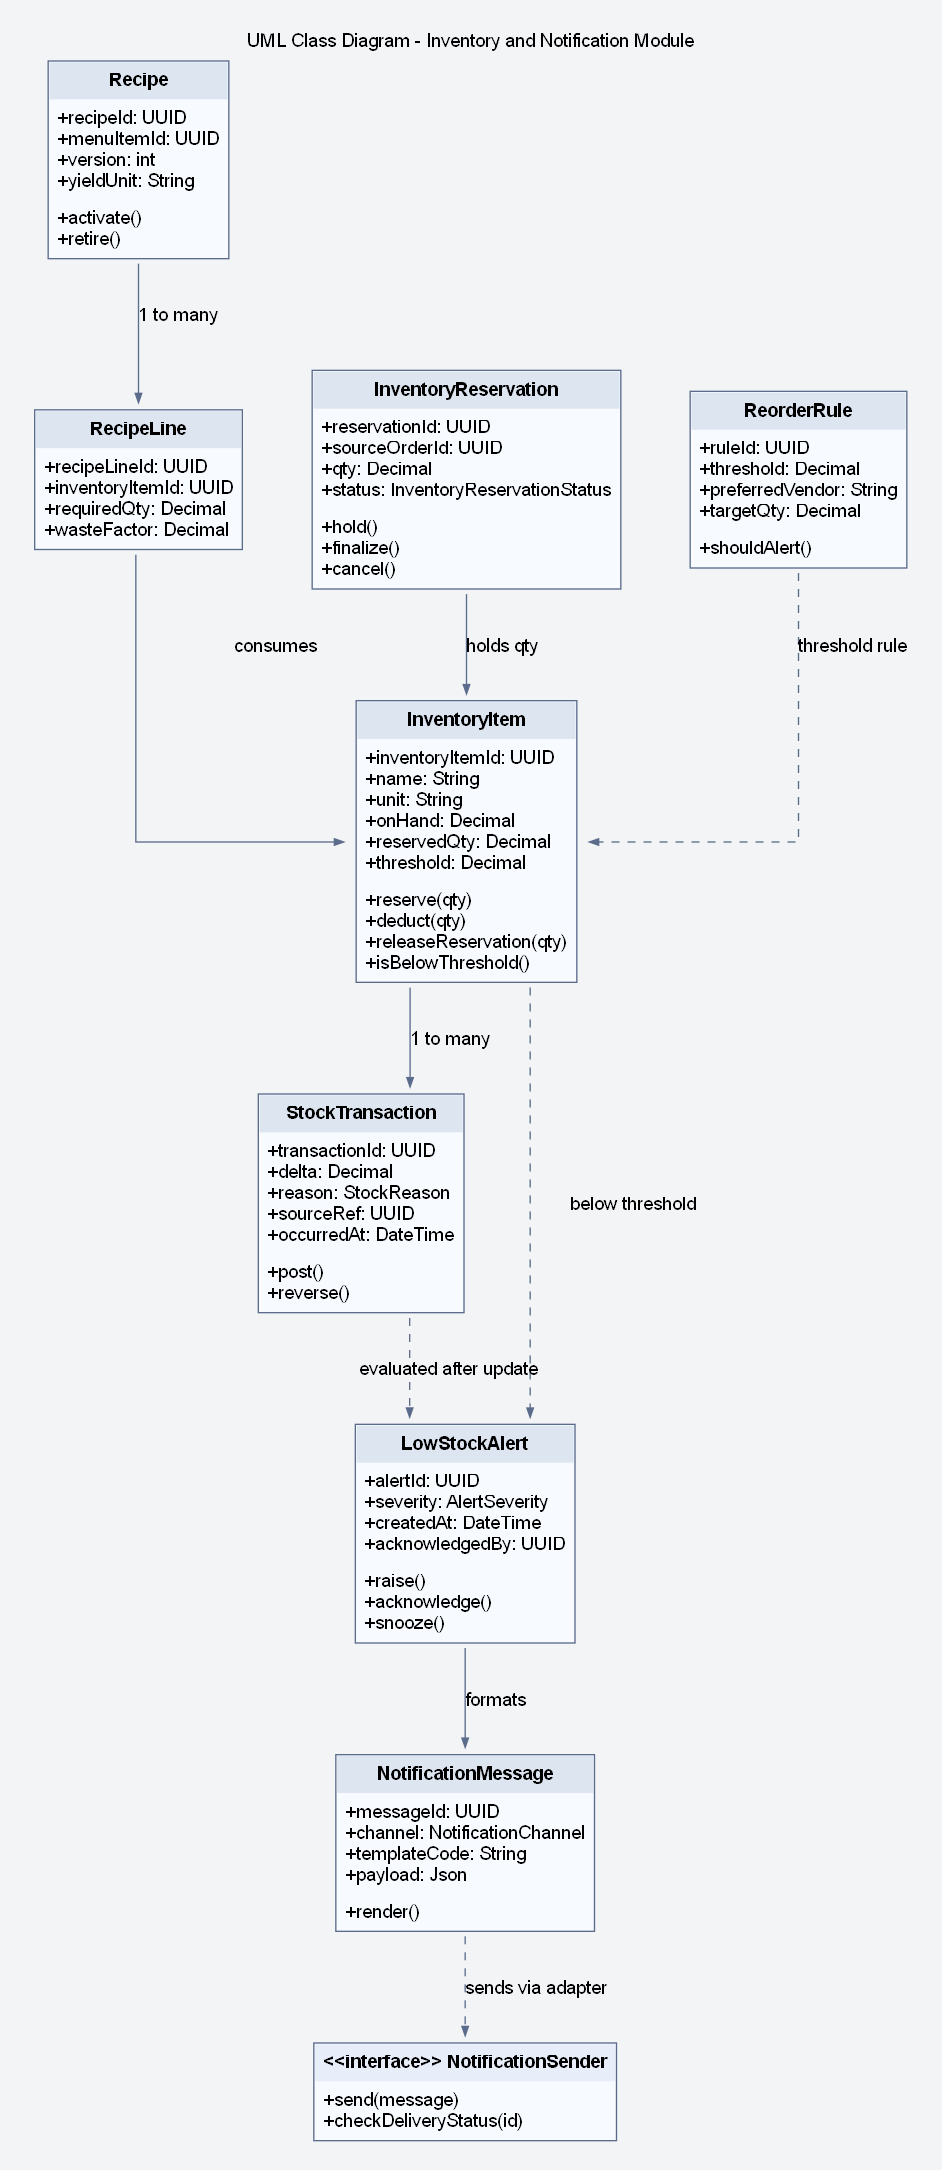
\includegraphics[width=0.97\linewidth,height=0.84\textheight,keepaspectratio]{30_uml_class_diagram_inventory_and_notification_module.png}
  }{
    \fbox{\parbox{0.82\linewidth}{Thiếu file \textsf{30\_uml\_class\_diagram\_inventory\_and\_notification\_module.(pdf/png)}.}}
  }
}
\caption{Sơ đồ lớp chi tiết cho module \textsf{inventory} và \textsf{notification}}
\label{fig:irms-class-inventory-module}
\end{figure}

Hình~\ref{fig:irms-class-inventory-module} nối \textsf{InventoryService}, \textsf{InventoryIngredientService}, \textsf{InventoryStockService} với workflow cảnh báo tồn kho và nhóm thông báo. \textsf{NotificationRequestedConsumer}, \textsf{NotificationRequestMaterializer} và các adapter kênh gửi được giữ vì chúng là class chính trong thiết kế và cũng xuất hiện ở C\&C View xử lý nền.

\begin{figure}[H]
\centering
\IfFileExists{31_uml_class_diagram_identity_audit_and_reporting_module.png}{
  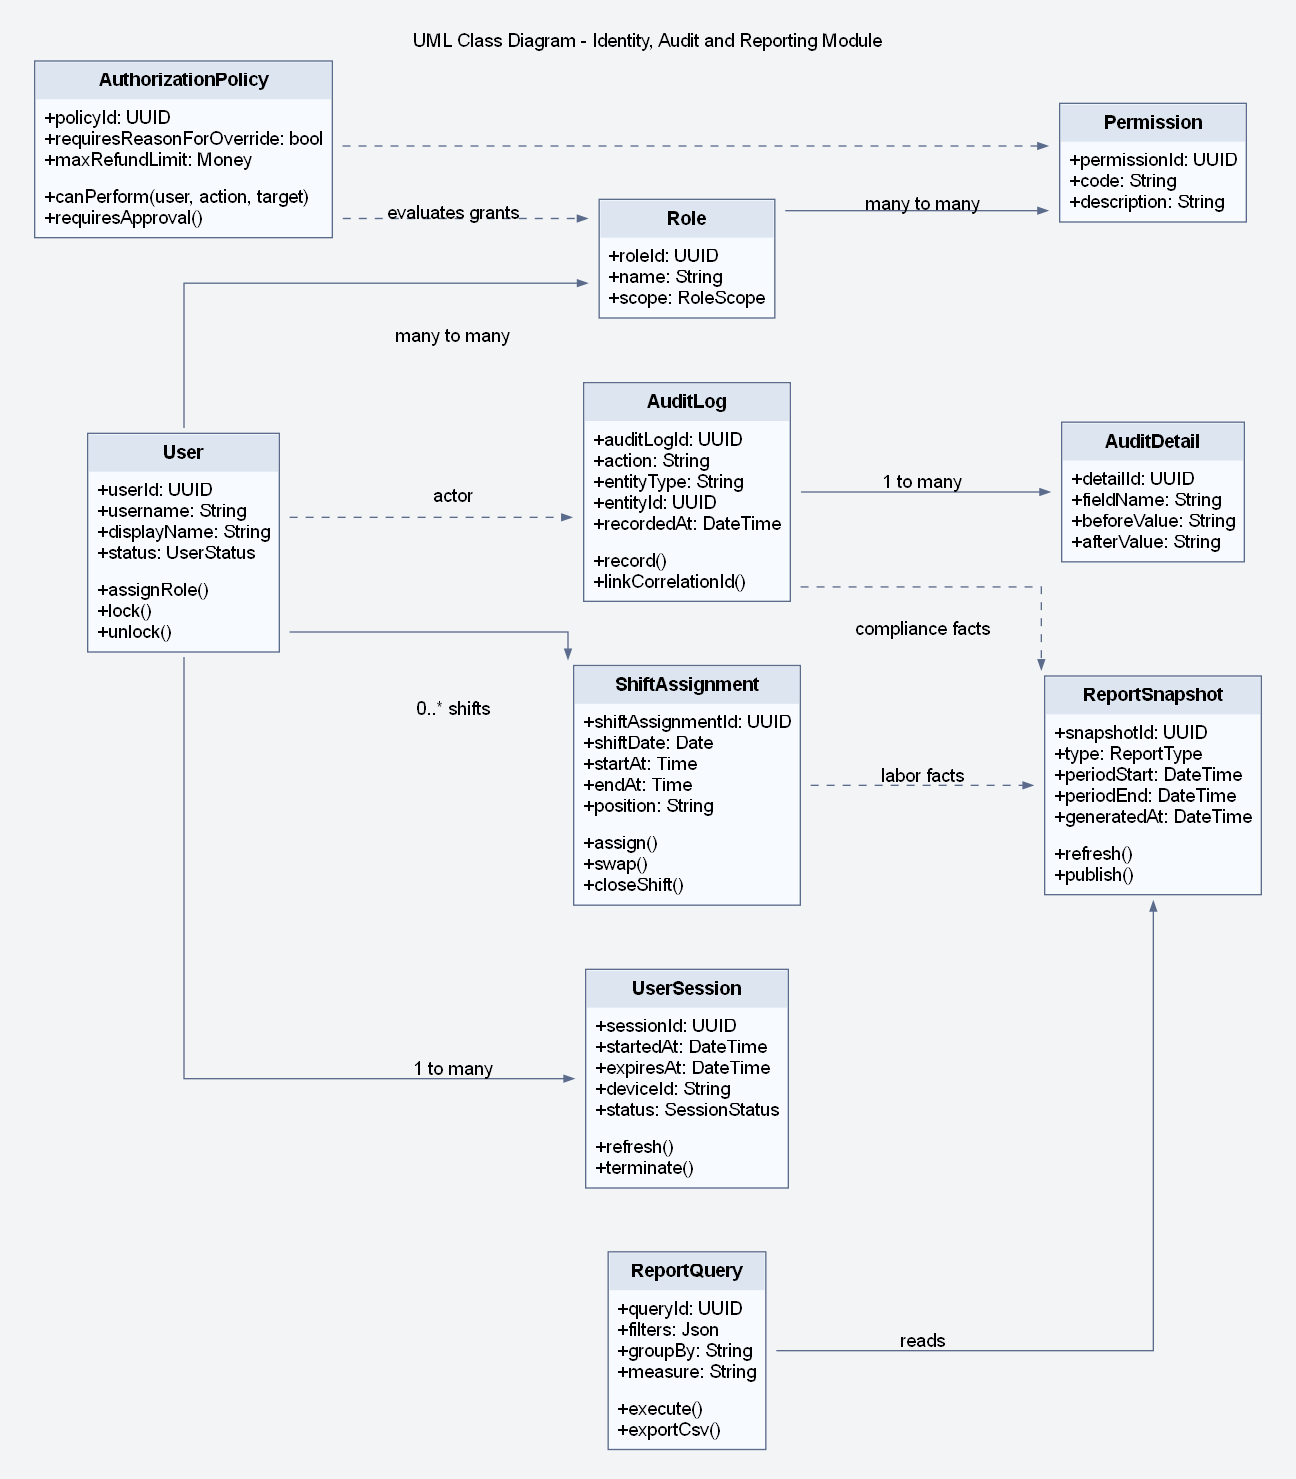
\includegraphics[width=0.97\linewidth,height=0.84\textheight,keepaspectratio]{31_uml_class_diagram_identity_audit_and_reporting_module.png}
}{
  \IfFileExists{31_uml_class_diagram_identity_audit_and_reporting_module.pdf}{
    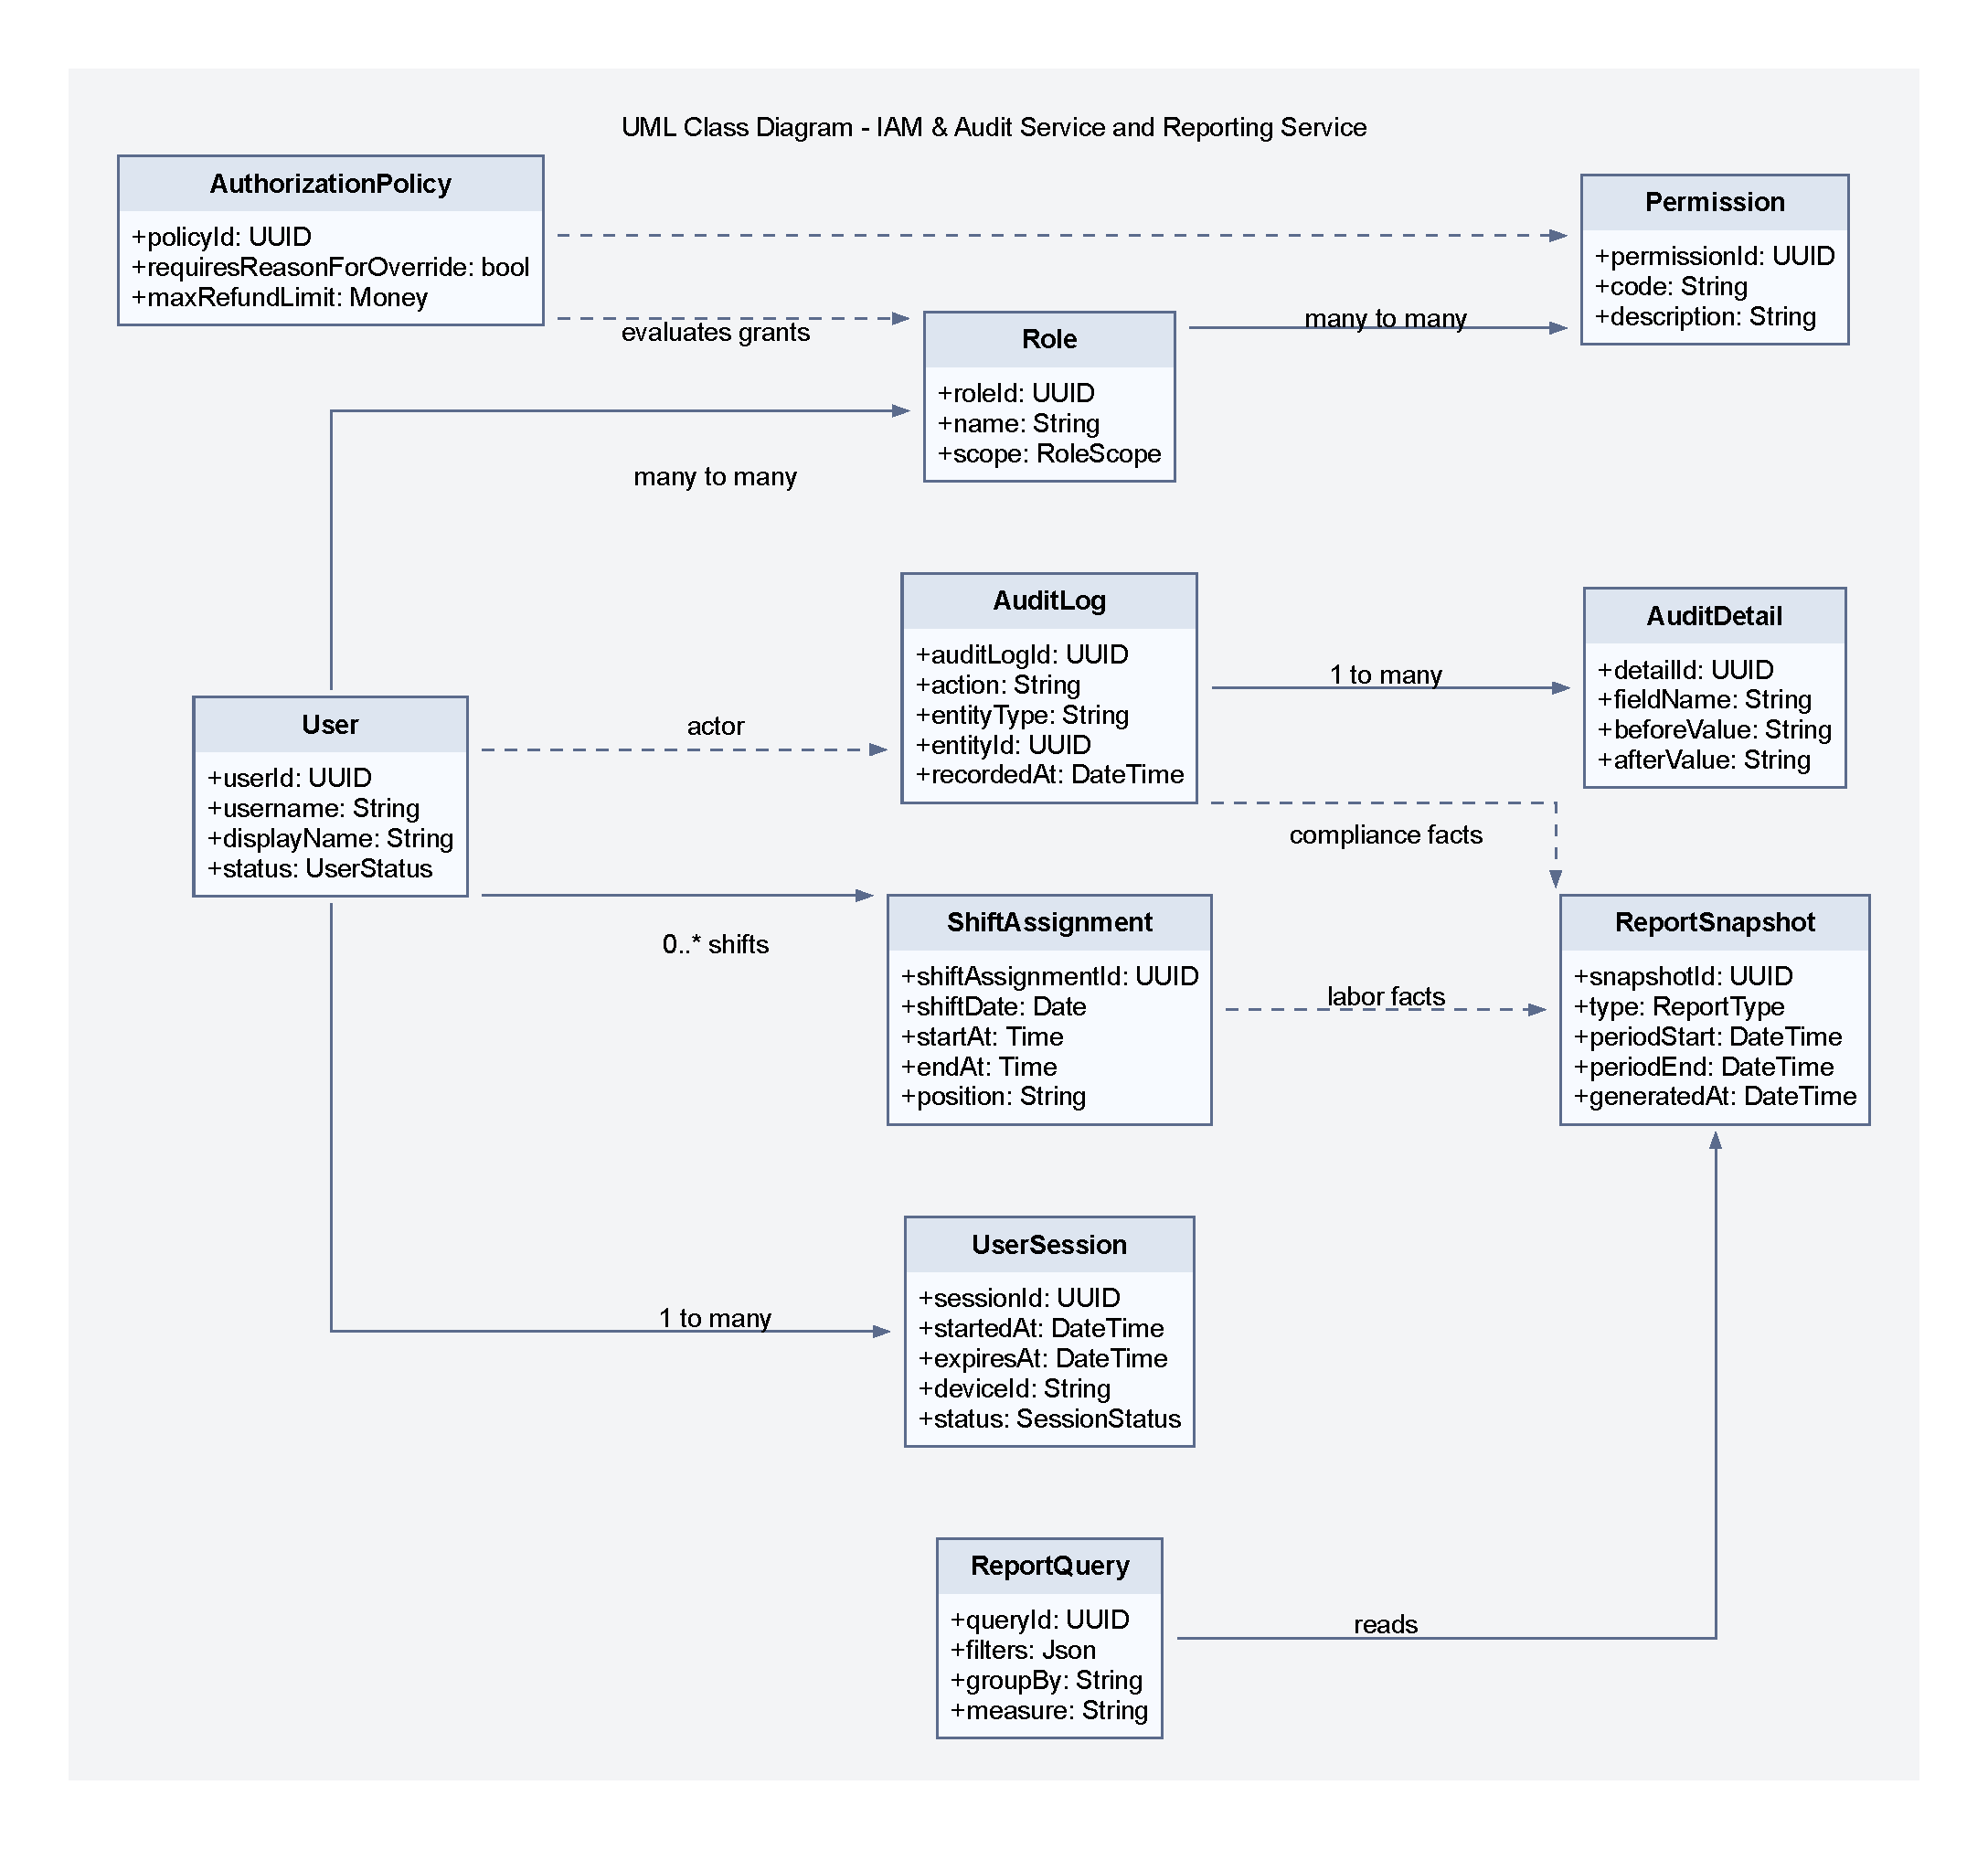
\includegraphics[width=0.97\linewidth,height=0.84\textheight,keepaspectratio]{31_uml_class_diagram_identity_audit_and_reporting_module.pdf}
  }{
    \fbox{\parbox{0.82\linewidth}{Thiếu file \textsf{31\_uml\_class\_diagram\_identity\_audit\_and\_reporting\_module.(png/pdf)}.}}
  }
}
\caption{Sơ đồ lớp chi tiết cho module \textsf{identity}, kiểm toán và \textsf{reporting}}
\label{fig:irms-class-governance-module}
\end{figure}

Hình~\ref{fig:irms-class-governance-module} mô tả vùng kiểm soát bằng các controller, service, phạm vi triển khaisitory và bộ xử lý sự kiện: \textsf{AuthController}, \textsf{AuditController}, \textsf{ReportingController}, \textsf{DashboardController}, \textsf{AuthService}, \textsf{AuditService}, \textsf{AuditEventMaterializer}, \textsf{AuditRecordingRequestedConsumer}, \textsf{ReportingQueryService} và \textsf{ReportingProjectionConsumer}. Quan hệ giữa kiểm toán/báo cáo với bộ xử lý sự kiện nhất quán với Component-and-Connector View: dữ liệu quản trị được cập nhật qua xử lý nền và phạm vi triển khaisitory/query service riêng.
\FloatBarrier
\subsection{Thiết kế hành vi}

\activitygroup{Nhóm đặt bàn và bàn ăn}

\activitydiagramfigure{uc-res-01-create-reservation}{Sơ đồ hoạt động cho UC-RES-01 -- Tạo đặt bàn}{fig:activity-uc-res-01-create-reservation}

\activitydiagramfigure{uc-res-02-checkin-and-seat}{Sơ đồ hoạt động cho UC-RES-02 -- Nhận khách và sắp bàn}{fig:activity-uc-res-02-checkin-and-seat}

\paragraph{Phân tích sơ đồ UC-RES-02.}

Luồng hoạt động trong trường hợp này bám sát thực tế tại quầy lễ tân: tìm đặt bàn, kiểm tra hiệu lực, đối chiếu số khách thực tế, xác định có cần đổi bàn hoặc ghép bàn hay không, sau đó mới mở \textsf{TableSession}. Điểm mấu chốt là việc \textbf{mở phiên phục vụ bàn} luôn diễn ra sau bước kiểm tra bàn khả dụng, nhờ đó báo cáo giữ được bất biến quan trọng rằng một bàn không có hai phiên phục vụ hoạt động cùng lúc.

Ngoài ra, sơ đồ cũng làm rõ nhánh ngoại lệ khi đặt bàn đã quá giờ giữ chỗ. Trong tình huống này, hệ thống không tự động bỏ qua mà chuyển sang bước phê duyệt của quản lý. 
\activitydiagramfigure{uc-res-03-manage-waitlist}{Sơ đồ hoạt động cho UC-RES-03 -- Quản lý danh sách chờ}{fig:activity-uc-res-03-manage-waitlist}

\activitydiagramfigure{uc-res-04-update-table-status-and-release}{Sơ đồ hoạt động cho UC-RES-04 -- Cập nhật trạng thái bàn và giải phóng bàn}{fig:activity-uc-res-04-update-table-status-and-release}

\paragraph{Phân tích sơ đồ UC-RES-04.}
\begin{itemize}
\item \textbf{Ràng buộc trạng thái \textsf{Available}:} Trạng thái bàn không cập nhật tự động sau thanh toán mà yêu cầu validation: đóng toàn bộ phiên phục vụ (\textsf{session}), tất toán công nợ (\textsf{billing}) và xác nhận hoàn tất vệ sinh (\textsf{cleaning}).
\item \textbf{Phối hợp liên module:} Đồng bộ hóa dữ liệu giữa ba miền nghiệp vụ: \textsf{TableSession}, \textsf{Billing} và \textsf{Waitlist}.
\item \textbf{Hiệu quả vận hành:} Đảm bảo tính nhất quán giữa hệ thống và thực tế, tránh lỗi gán trùng bàn (double-booking) và cung cấp dữ liệu chính xác để tính toán hiệu suất vòng quay bàn.
\end{itemize}
\activitydiagramfigure{uc-res-05-notify-customer}{Sơ đồ hoạt động cho UC-RES-05 -- Gửi thông báo cho khách hàng}{fig:activity-uc-res-05-notify-customer}

\paragraph{Phân tích sơ đồ UC-RES-05.}
\begin{itemize}
\item \textbf{Controlled Side-effect}: Thông báo là hệ quả có kiểm soát phát sinh từ các sự kiện nghiệp vụ (xác nhận đặt bàn, nhắc giờ, gọi khách từ waitlist).
\item \textbf{Quản lý luồng}: Mỗi thông báo có đầu vào, điều kiện kích hoạt và trạng thái xử lý riêng biệt.
\item \textbf{Phân tách trách nhiệm}: Cô lập logic nghiệp vụ (\textsf{Core Domain}) khỏi các chi tiết hạ tầng (\textsf{Notification Adapter}) và các cơ chế vận hành kỹ thuật (\textsf{Retry}, \textsf{Fallback}).
\end{itemize}
\activitygroup{Nhóm gọi món và điều phối bếp}

\activitydiagramfigure{uc-ord-01-create-table-order}{Sơ đồ hoạt động cho UC-ORD-01 -- Tạo đơn gọi món tại bàn}{fig:activity-uc-ord-01-create-table-order}

\paragraph{Phân tích sơ đồ UC-ORD-01.}
Luồng hoạt động gọi món bao gồm các bước: tải thực đơn, kiểm tra quyền thao tác trên phiên bàn, chọn món, kiểm tra trạng thái còn bán (quay lại chọn lại nếu hết hàng), tính tạm tính và rẽ nhánh \enquote{lưu nháp} hoặc \enquote{xác nhận đơn}. Thao tác này đóng vai trò chốt trạng thái (snapshot) về giá và tính hợp lệ của món ngay tại thời điểm xử lý.

Sơ đồ cũng vạch rõ ranh giới trách nhiệm giữa hai module:
\begin{itemize}
    \item \textbf{\textsf{Ordering}:} Giới hạn ở việc tạo và xác nhận đơn gọi món.
    \item \textbf{\textsf{Kitchen Coordination}:} Tách biệt hoàn toàn việc tạo phiếu bếp và điều phối sang trạm bếp (thuộc một sơ đồ riêng).
\end{itemize}
\activitydiagramfigure{uc-ord-02-customize-item-and-allergy-note}{Sơ đồ hoạt động cho UC-ORD-02 -- Tùy biến món và ghi chú dị ứng}{fig:activity-uc-ord-02-customize-item-and-allergy-note}

\activitydiagramfigure{uc-ord-03-send-order-to-kitchen}{Sơ đồ hoạt động cho UC-ORD-03 -- Gửi đơn gọi món sang bếp}{fig:activity-uc-ord-03-send-order-to-kitchen}

\paragraph{Phân tích sơ đồ UC-ORD-03.}
Sơ đồ mô tả ranh giới giao tiếp giữa hai module \textsf{Ordering} (gọi món) và \textsf{Kitchen Coordination} (điều phối bếp), bao gồm:

\begin{itemize}
    \item \textbf{Luồng xử lý chính:} Kiểm tra điều kiện $\rightarrow$ Phân loại món (làm ngay/làm sau) $\rightarrow$ Định tuyến theo trạm bếp (Station Routing) $\rightarrow$ Khởi tạo \textsf{KitchenTicket} $\rightarrow$ Đưa vào hàng đợi ưu tiên (Priority Queuing) $\rightarrow$ Cập nhật trạng thái đơn (\textsf{Order}).
    \item \textbf{Xử lý ngoại lệ (Exception Handling):} Nếu lỗi định tuyến trạm hoặc hệ thống màn hình bếp (KDS) offline, hệ thống đẩy request vào hàng đợi gửi lại (retry queue) và phát cảnh báo (alert) cho nhân viên. 
    \item \textbf{Đáp ứng NFR:} Cơ chế xử lý lỗi này đảm bảo yêu cầu phi chức năng về độ tin cậy (Reliability) và toàn vẹn dữ liệu (Data Integrity), tuyệt đối không làm mất các \textsf{KitchenTicket} đã được xác nhận.
\end{itemize}
\activitydiagramfigure{uc-kit-01-update-cooking-progress}{Sơ đồ hoạt động cho UC-KIT-01 -- Cập nhật tiến độ chế biến}{fig:activity-uc-kit-01-update-cooking-progress}

\paragraph{Phân tích sơ đồ UC-KIT-01.}
Luồng hoạt động bám sát quy trình xử lý thực tế tại trạm bếp:

\begin{itemize}
    \item \textbf{Luồng xử lý chính:} Nhận phiếu (\textsf{KitchenTicket}) $\rightarrow$ Kiểm tra trạm đích $\rightarrow$ Bắt đầu chế biến $\rightarrow$ Ghi nhận thời gian (timestamp) qua mỗi lần chuyển trạng thái $\rightarrow$ Đánh giá nguy cơ trễ hạn (delay risk) $\rightarrow$ Xác nhận hoàn tất (\textsf{Ready}). Việc lưu vết timestamp chi tiết là cơ sở dữ liệu bắt buộc để phục vụ module phân tích hiệu suất vận hành (operational analytics) sau này.
    
    \item \textbf{Xử lý ngoại lệ (Thiếu nguyên liệu/Sự cố):} Hệ thống không được phép kết thúc ngầm (fail silently). Request bắt buộc chuyển sang trạng thái chặn (\textsf{Blocked}), đồng thời phát cảnh báo (alert) và phản hồi trạng thái (feedback) về khu vực phục vụ. Cơ chế này đảm bảo luồng giao tiếp hai chiều giữa bếp và phục vụ luôn đồng bộ và nhất quán với kiến trúc tổng thể.
\end{itemize}
\activitydiagramfigure{uc-kit-02-serve-dishes}{Sơ đồ hoạt động cho UC-KIT-02 -- Ra món cho bàn}{fig:activity-uc-kit-02-serve-dishes}

\activitydiagramfigure{uc-kit-03-prioritize-kitchen-queue}{Sơ đồ hoạt động cho UC-KIT-03 -- Ưu tiên hàng chờ bếp và xử lý món gấp}{fig:activity-uc-kit-03-prioritize-kitchen-queue}

\paragraph{Phân tích sơ đồ UC-KIT-03.}
Luồng hoạt động định hình lại vai trò của hệ thống KDS: không chỉ hiển thị thụ động mà phải trực tiếp \textbf{điều phối thứ tự thực thi (queue prioritization)}.

\begin{itemize}
    \item \textbf{Tiêu chí phân luồng:} Trong giờ cao điểm, các \textsf{KitchenTicket} được sắp xếp tự động dựa trên: cam kết thời gian (SLA), cấu trúc món (course), phân hạng khách (VIP) và nguy cơ trễ hạn. Ca sử dụng này được tách độc lập để đáp ứng đúng yêu cầu \enquote{prioritize queues}.
    
    \item \textbf{Kiểm soát chính sách (Policy-driven):} Các can thiệp thay đổi thứ tự chế biến bắt buộc phải tuân thủ chính sách: yêu cầu phân quyền hợp lệ và ghi nhận lý do thay đổi (reason log), không cho phép tùy chỉnh tự do.
    
    \item \textbf{Khả năng truy vết (Traceability):} Cơ chế kiểm soát chặt chẽ giúp vận hành linh hoạt nhưng vẫn đảm bảo lưu vết (audit) đầy đủ để đối soát khi xảy ra khiếu nại về việc lên món sai thứ tự hoặc trễ SLA.
\end{itemize}
\activitydiagramfigure{uc-ord-04-edit-or-cancel-item}{Sơ đồ hoạt động cho UC-ORD-04 -- Sửa hoặc hủy dòng món}{fig:activity-uc-ord-04-edit-or-cancel-item}

\activitygroup{Nhóm hóa đơn, thanh toán và biên lai}

\activitydiagramfigure{uc-bil-01-create-bill}{Sơ đồ hoạt động cho UC-BIL-01 -- Tạo hóa đơn cho bàn}{fig:activity-uc-bil-01-create-bill}

\paragraph{Phân tích sơ đồ UC-BIL-01.}
\begin{itemize}
\item \textbf{Cơ chế Preview:} Bước \enquote{xem trước hóa đơn} đóng vai trò chốt chặn cuối cùng để kiểm tra tính nhất quán dữ liệu, phòng ngừa sai sót do các thay đổi tức thời (hủy món hoặc cập nhật giá).
\item \textbf{Ràng buộc nghiệp vụ:} Hệ thống thiết lập nhánh chặn phát hành khi dữ liệu không hợp lệ. Điều này khẳng định \textsf{Bill} là một thực thể nghiệp vụ (business entity) có các điều kiện phát hành và chuyển đổi trạng thái chặt chẽ, không đơn thuần là phép cộng tổng dữ liệu.
\end{itemize}
\activitydiagramfigure{uc-bil-02-split-bill-and-tip}{Sơ đồ hoạt động cho UC-BIL-02 -- Tách hóa đơn và thêm tiền boa}{fig:activity-uc-bil-02-split-bill-and-tip}

\activitydiagramfigure{uc-pay-01-process-payment}{Sơ đồ hoạt động cho UC-PAY-01 -- Xử lý thanh toán}{fig:activity-uc-pay-01-process-payment}

\paragraph{Phân tích sơ đồ UC-PAY-01.}
\begin{itemize}
    \item \textbf{Phân luồng thanh toán:}
    \begin{itemize}
        \item \textsf{PaymentGateway}: Tạo yêu cầu giao dịch $\rightarrow$ Nhận kết quả $\rightarrow$ Lưu mã tham chiếu $\rightarrow$ Xử lý các trạng thái: thành công, thất bại, hoặc chờ rà soát.
        \item \textbf{Tiền mặt}: Tính tiền thối và cập nhật số dư còn lại của hóa đơn.
    \end{itemize}
    \item \textbf{Logic tất toán:} Sau khi ghi nhận, hệ thống kiểm tra số tiền đã thanh toán:
    \begin{itemize}
        \item \textbf{Chưa đủ}: Hóa đơn giữ trạng thái mở (\textsf{OPEN}).
        \item \textbf{Đã đủ}: Đóng hóa đơn (\textsf{CLOSED}) và kích hoạt luồng phát hành biên lai.
    \end{itemize}
\end{itemize}
\activitydiagramfigure{uc-pay-02-issue-receipt}{Sơ đồ hoạt động cho UC-PAY-02 -- Phát hành biên lai}{fig:activity-uc-pay-02-issue-receipt}

\activitydiagramfigure{uc-pay-03-refund}{Sơ đồ hoạt động cho UC-PAY-03 -- Hoàn tiền}{fig:activity-uc-pay-03-refund}

\paragraph{Phân tích sơ đồ UC-PAY-03.}
Sơ đồ hoàn tiền hiện đã thể hiện đầy đủ các điểm kiểm soát bắt buộc:

\begin{itemize}
    \item Chọn giao dịch gốc
    \item Kiểm tra số tiền còn được hoàn
    \item Nhập lý do hoàn tiền
    \item So sánh với ngưỡng phê duyệt
    \item Xin xác nhận của quản lý nếu cần
    \item Xử lý hoàn tiền qua \textsf{PaymentGateway} hoặc ghi nhận hoàn tiền thủ công
    \item Cập nhật sổ kiểm toán
\end{itemize}

Điều này rất quan trọng vì hoàn tiền là thao tác nhạy cảm nhất trong vùng thanh toán.

Một chi tiết đáng chú ý là sơ đồ đã tách rõ nhánh \enquote{chờ rà soát} khi \textsf{PaymentGateway} không chấp nhận hoặc phản hồi không rõ ràng. Nhờ đó báo cáo có thể giải thích trạng thái nghiệp vụ chặt chẽ hơn, thay vì gom mọi trường hợp không thành công vào một nhãn lỗi duy nhất.
\activitygroup{Nhóm tồn kho, cảnh báo và phân tích}

\activitydiagramfigure{uc-inv-01-update-stock-consumption}{Sơ đồ hoạt động cho UC-INV-01 -- Cập nhật tiêu hao tồn kho sau phục vụ}{fig:activity-uc-inv-01-update-stock-consumption}

\paragraph{Phân tích sơ đồ UC-INV-01.}
Sơ đồ cập nhật tiêu hao tồn kho phản ánh đúng bản chất suy diễn của vùng tồn kho. Các bước xử lý bao gồm:

\begin{itemize}
    \item Nhận sự kiện từ món đã phục vụ hoặc điều chỉnh thủ công
    \item Tra công thức nguyên liệu
    \item Tính lượng tiêu hao theo số lượng món
    \item Sinh \textsf{StockTransaction} theo từng nguyên liệu
    \item Cập nhật số lượng tồn hiện có
    \item Đánh giá các điều kiện bất thường
\end{itemize}

Sơ đồ cũng làm rõ hai nhánh ngoại lệ quan trọng:

\begin{itemize}
    \item Thiếu ánh xạ công thức
    \item Âm kho bất thường
\end{itemize}

Nhờ đó phần thiết kế hành vi bám sát hơn với ca sử dụng đã đặc tả, đồng thời nối được với sơ đồ cảnh báo sắp hết hàng ngay bên dưới.
\activitydiagramfigure{uc-inv-02-low-stock-alert}{Sơ đồ hoạt động cho UC-INV-02 -- Nhận cảnh báo sắp hết hàng}{fig:activity-uc-inv-02-low-stock-alert}

\activitydiagramfigure{uc-inv-03-reorder-recommendation}{Sơ đồ hoạt động cho UC-INV-03 -- Phân tích tiêu hao và đề xuất nhập hàng}{fig:activity-uc-inv-03-reorder-recommendation}

\paragraph{Phân tích sơ đồ UC-INV-03.}

Use case này giúp phần tồn kho bám sát hơn với yêu cầu \enquote{historical usage helps predict reorder quantities and manage waste}. Nếu chỉ dừng ở cập nhật tiêu hao và cảnh báo sắp hết hàng, IRMS mới chỉ hỗ trợ phản ứng vận hành ngắn hạn, chưa đủ để ra quyết định chuẩn bị hàng hóa theo chu kỳ ngày, tuần hoặc mùa cao điểm. Do đó, sơ đồ này chuyển trọng tâm của vùng tồn kho từ \textbf{theo dõi hiện trạng} sang \textbf{hỗ trợ ra quyết định}.

Điểm đáng chú ý là sơ đồ không mô tả dự báo như một thuật toán mơ hồ mà chỉ rõ các dữ liệu đầu vào gồm tiêu hao lịch sử, cảnh báo sắp hết hàng, hao hụt, lead time và mức tồn an toàn. Nhờ đó, đề xuất nhập hàng được thể hiện là kết quả của mô hình dữ liệu và luồng xử lý đã có sẵn, không phải một chức năng bổ sung rời rạc thiếu nền dữ liệu đủ tin cậy.\activitydiagramfigure{uc-rep-01-view-revenue-and-operations-report}{Sơ đồ hoạt động cho UC-REP-01 -- Xem báo cáo doanh thu và vận hành}{fig:activity-uc-rep-01-view-revenue-and-operations-report}

\activitygroup{Nhóm quản trị cấu hình và vận hành}

\activitydiagramfigure{uc-adm-01-manage-menu-and-pricing}{Sơ đồ hoạt động cho UC-ADM-01 -- Quản lý thực đơn và giá bán}{fig:menu}
\begin{itemize}
    \item Quản lý mở màn hình cấu hình thực đơn và chọn món hoặc danh mục cần chỉnh sửa.
    
    \item Hệ thống hiển thị thông tin chi tiết của món, bao gồm giá, trạng thái và các chương trình khuyến mãi hiện tại.
    
    \item Quản lý thực hiện chỉnh sửa thông tin món và có thể áp dụng khuyến mãi nếu cần.
    
    \item Khi lưu thay đổi, quản lý gửi cấu hình món, giá, trạng thái bán, khuyến mãi hoặc công thức nguyên liệu theo form hiện tại.
    
    \item Hệ thống kiểm tra dữ liệu cấu hình:
    \begin{itemize}
        \item Nếu thiếu thông tin bắt buộc, hệ thống yêu cầu bổ sung trước khi tiếp tục.
        \item Nếu danh mục không tồn tại hoặc công thức nguyên liệu sai định dạng, hệ thống yêu cầu điều chỉnh trước khi lưu.
    \end{itemize}
    
    \item Khi dữ liệu hợp lệ, hệ thống lưu thay đổi thực đơn, công thức liên quan và ghi nhận dấu vết kiểm toán; nếu trạng thái bán thay đổi, hệ thống phát event cập nhật khả dụng.
    
    \item Các đơn hàng đang mở vẫn giữ nguyên giá đã ghi nhận trước đó để đảm bảo tính nhất quán.
\end{itemize}
\activitydiagramfigure{uc-adm-02-manage-roles-and-permissions}{Sơ đồ hoạt động cho UC-ADM-02 -- Quản lý vai trò và phân quyền}{fig:role}
\begin{itemize}
    \item Quản trị viên mở màn hình quản lý người dùng và tìm kiếm người dùng cần cập nhật quyền.
    
    \item Hệ thống hiển thị vai trò và danh sách quyền hiện tại của người dùng.
    
    \item Quản trị viên thực hiện gán hoặc điều chỉnh vai trò và quyền theo chính sách RBAC.
    
    \item Hệ thống xử lý các trường hợp mở rộng:
    \begin{itemize}
        \item Nếu không còn vai trò nào được chọn, hệ thống chặn thao tác vì mỗi nhân viên phải giữ ít nhất một vai trò.
        \item Nếu vai trò được chọn không tồn tại trong danh sách hiện hành, hệ thống chặn thao tác và yêu cầu chọn lại.
    \end{itemize}
    
    \item Hệ thống kiểm tra tính hợp lệ của chính sách phân quyền:
    \begin{itemize}
        \item Nếu phát hiện xung đột chính sách RBAC, hệ thống yêu cầu quản trị viên điều chỉnh lại quyền.
        \item Nếu thao tác dẫn đến việc gỡ bỏ quyền quản trị cuối cùng, hệ thống chặn thao tác để đảm bảo luôn tồn tại ít nhất một tài khoản quản trị.
    \end{itemize}
    
    \item Khi dữ liệu hợp lệ, hệ thống thay thế danh sách vai trò của người dùng bằng các vai trò đã chọn.
    
    \item Hệ thống yêu cầu người dùng đăng nhập lại để áp dụng quyền mới.
    
    \item Cuối cùng, hệ thống ghi nhận toàn bộ thay đổi vào nhật ký kiểm toán nhằm phục vụ truy vết và kiểm soát.
\end{itemize}
\activitydiagramfigure{uc-adm-03-review-audit-log}{Sơ đồ hoạt động cho UC-ADM-03 -- Xem nhật ký kiểm toán và truy vết thao tác nhạy cảm}{fig:log}
\begin{itemize}
    \item Người dùng có thẩm quyền mở màn hình nhật ký kiểm toán để thực hiện tra cứu.
    
    \item Hệ thống kiểm tra quyền truy cập:
    \begin{itemize}
        \item Nếu không đủ quyền, hệ thống từ chối truy cập hoặc chỉ hiển thị dữ liệu rút gọn.
        \item Nếu hợp lệ, hệ thống cho phép tiếp tục truy vấn.
    \end{itemize}
    
    \item Người dùng nhập bộ lọc tìm kiếm (thời gian, người thao tác, loại hành động, mã liên kết).
    
    \item Hệ thống truy vấn và hiển thị danh sách nhật ký kiểm toán:
    \begin{itemize}
        \item Nếu không có dữ liệu phù hợp, hệ thống thông báo và yêu cầu điều chỉnh bộ lọc.
        \item Nếu người dùng không đủ quyền, hệ thống làm mờ hoặc ẩn thông tin nhạy cảm.
    \end{itemize}
    
    \item Người dùng chọn một bản ghi để xem chi tiết, bao gồm giá trị trước và sau thay đổi, lý do và ngữ cảnh thực hiện.
    
    \item Người dùng có thể xuất báo cáo hoặc đánh dấu bản ghi cần theo dõi.
    
    \item Hệ thống ghi nhận hành vi truy cập và thao tác trên nhật ký kiểm toán nhằm phục vụ kiểm soát và truy vết sau này.
\end{itemize}
\activitydiagramfigure{uc-ops-01-manage-staff-shifts}{Sơ đồ hoạt động cho UC-OPS-01 -- Quản lý ca làm nhân viên}{fig:calamviec}
\begin{itemize}
    \item Quản lý mở màn hình lịch làm việc và chọn ngày, khu vực cùng loại ca cần phân công.
    
    \item Hệ thống hiển thị danh sách nhân viên và các ca làm việc đã có.
    
    \item Quản lý thực hiện gán nhân viên vào ca và khu vực làm việc.
    
    \item Hệ thống hỗ trợ các trường hợp mở rộng:
    \begin{itemize}
        \item Nếu thời điểm kết thúc không sau thời điểm bắt đầu, hệ thống chặn lưu ca.
        \item Nếu nhân viên đã có ca trùng khoảng thời gian, hệ thống chặn lưu ca và yêu cầu chọn lại.
    \end{itemize}
    
    \item Hệ thống kiểm tra các ràng buộc lập lịch:
    \begin{itemize}
        \item Nếu phát hiện trùng ca, hệ thống chặn lưu và yêu cầu điều chỉnh.
        \item Nếu dữ liệu hợp lệ, hệ thống lưu \textsf{ShiftAssignment}, ghi nhật ký kiểm toán và đưa thông báo nội bộ vào hàng chờ cho nhân viên.
    \end{itemize}
    
    \item Khi dữ liệu hợp lệ, quản lý lưu lịch làm việc.
    
    \item Hệ thống cập nhật \textsf{ShiftAssignment}, ghi nhật ký kiểm toán và đưa thông báo nội bộ vào hàng chờ cho nhân viên liên quan.
\end{itemize}
\pagebreak


\appendix
\section{Phụ lục}
\label{appendix:overall}

\subsection{Lý do lựa chọn kiến trúc và hồ sơ quyết định kiến trúc}\label{appendix:architecture-rationale}

Các quyết định kiến trúc của IRMS được đặt trên ba cơ sở: bối cảnh vận hành của nhà hàng, yêu cầu chức năng theo từng miền nghiệp vụ và yêu cầu phi chức năng ở mức toàn dự án. Kiến trúc chủ đạo là \textbf{service-based architecture theo miền nghiệp vụ}; \textbf{event-driven processing} đóng vai trò bổ trợ cho các hệ quả nền như thông báo, cập nhật mô hình đọc báo cáo, kiểm toán và cảnh báo tồn kho. Cách lựa chọn này giữ tuyến giao dịch chính ngắn, đồng thời vẫn cho phép các hoạt động hỗ trợ được xử lý linh hoạt phía sau.

\subsubsection{So sánh các kiểu kiến trúc ứng viên}

{\small
\setlength{\LTleft}{0pt}
\setlength{\LTright}{0pt}
\renewcommand{\arraystretch}{1.15}
\begin{longtable}{>{\raggedright\arraybackslash}p{3.1cm} >{\raggedright\arraybackslash}p{4.5cm} >{\raggedright\arraybackslash}p{6.4cm}}
\caption{So sánh các kiểu kiến trúc ứng viên cho IRMS}\label{tab:appendix-architecture-candidates}\\
\toprule
\textbf{Kiểu kiến trúc} & \textbf{Điểm phù hợp} & \textbf{Giới hạn trong bối cảnh IRMS} \\
\midrule
\endfirsthead
\toprule
\textbf{Kiểu kiến trúc} & \textbf{Điểm phù hợp} & \textbf{Giới hạn trong bối cảnh IRMS} \\
\midrule
\endhead
Kiến trúc phân lớp tập trung thuần & Dễ khởi tạo và đơn giản cho các thao tác nội bộ. & Dễ gom các nghiệp vụ khác bản chất vào cùng một tầng kỹ thuật, làm mờ ranh giới giữa đặt bàn, gọi món, bếp, thanh toán, tồn kho và báo cáo. \\
\addlinespace
Service-based theo miền nghiệp vụ & Phù hợp với cách IRMS chia trách nhiệm theo các năng lực vận hành của nhà hàng; mỗi service có ranh giới và hợp đồng giao tiếp rõ hơn. & Cần quản lý chặt hợp đồng giữa các service và tránh phụ thuộc vòng giữa các miền nghiệp vụ. \\
\addlinespace
Microservices đầy đủ & Cô lập mạnh về triển khai và hỗ trợ vòng đời phát hành riêng. & Chi phí vận hành, giám sát, quản trị giao dịch phân tán và quản lý hợp đồng dịch vụ cao hơn nhu cầu của phạm vi hiện tại. \\
\addlinespace
Event-driven thuần & Phù hợp cho phát tán sự kiện, xử lý nền và cập nhật mô hình đọc. & Không phù hợp cho toàn bộ hệ thống vì tạo đơn, lập hóa đơn, thanh toán và hoàn tiền cần phản hồi tức thời và trạng thái lỗi rõ ràng. \\
\addlinespace
Service-based kết hợp event-driven & Giữ ranh giới nghiệp vụ bằng service-based architecture, đồng thời dùng event-driven cho các hệ quả nền như thông báo, báo cáo, kiểm toán và cảnh báo tồn kho. & Cần phân biệt rõ thao tác nào đồng bộ, thao tác nào bất đồng bộ; các luồng nền cần chống xử lý lặp và có khả năng theo dõi trạng thái. \\
\bottomrule
\end{longtable}
\normalsize
}

Từ các phương án trên, service-based architecture là cấu trúc chính vì bám sát các miền trách nhiệm đã nêu trong Chương~1. Event-driven processing không thay thế cấu trúc này mà bổ sung một cơ chế phối hợp cho các hệ quả không cần chặn thao tác của nhân viên. Sự kết hợp này tạo ra một kiến trúc vừa rõ ràng ở tuyến giao dịch chính, vừa đủ linh hoạt cho thông báo, báo cáo, kiểm toán và cảnh báo tồn kho.

\subsubsection{Hồ sơ quyết định kiến trúc}

\begin{adrbox}[title={ADR-0001: Kiến trúc chủ đạo}]
\begin{description}[leftmargin=3.0cm,style=nextline]
  \item[Quyết định] Chọn \textbf{service-based architecture theo miền nghiệp vụ} làm kiến trúc chính; dùng \textbf{event-driven processing} cho các tác vụ nền và hệ quả phụ.
  \item[Cơ sở lựa chọn] Gọi món, điều phối bếp và thanh toán cần phản hồi nhanh, trong khi báo cáo, thông báo, kiểm toán và cảnh báo tồn kho có thể xử lý sau giao dịch chính.
  \item[Hệ quả] Kiến trúc phải phân biệt rõ luồng đồng bộ và bất đồng bộ; các luồng nền cần chống xử lý lặp, hỗ trợ thử lại và có mã liên kết để truy vết.
  \item[Không chọn] Kiến trúc phân lớp tập trung làm mờ ranh giới nghiệp vụ; microservices đầy đủ vượt quá mức cần thiết; event-driven thuần không phù hợp với thao tác cần phản hồi tức thời.
\end{description}
\end{adrbox}

\begin{adrbox}[title={ADR-0002: Điểm vào thống nhất}]
\begin{description}[leftmargin=3.0cm,style=nextline]
  \item[Quyết định] Dùng \textsf{Frontend Node Server} để phục vụ giao diện React và chuyển tiếp \textsf{/api}; backend dùng \textsf{API Gateway} làm điểm vào chung cho các service.
  \item[Cơ sở lựa chọn] IRMS có nhiều màn hình vận hành như gọi món, bếp, thu ngân và quản lý. Các giao diện này cần một điểm vào ổn định thay vì phụ thuộc vào vị trí của từng service nội bộ.
  \item[Hệ quả] Giao tiếp ở biên hệ thống được chuẩn hóa; thay đổi bên trong backend ít ảnh hưởng đến giao diện người dùng.
\end{description}
\end{adrbox}

\begin{adrbox}[title={ADR-0003: REST, RabbitMQ và Outbox}]
\begin{description}[leftmargin=3.0cm,style=nextline]
  \item[Quyết định] Dùng \textsf{REST} đồng bộ cho thao tác tuyến đầu; dùng \textsf{RabbitMQ}, \textsf{outbox\_events}, \textsf{processed\_events} và bộ xử lý nền cho các tác vụ sau giao dịch.
  \item[Cơ sở lựa chọn] Tạo đơn, lập hóa đơn và thanh toán cần phản hồi tức thời. Gửi thông báo, cập nhật báo cáo, ghi kiểm toán và xử lý lại khi lỗi không nên làm dài tuyến giao dịch chính.
  \item[Hệ quả] Cần kiểm soát thời điểm phát sự kiện sau giao dịch, tránh xử lý lặp và quan sát được trạng thái của hàng đợi.
  \item[Ví dụ] Tuyến đồng bộ gồm tạo đơn, lập hóa đơn và thanh toán. Tuyến bất đồng bộ gồm \textsf{OrderConfirmed}, \textsf{LowStockDetected} và yêu cầu làm mới báo cáo.
\end{description}
\end{adrbox}

\begin{adrbox}[title={ADR-0004: PostgreSQL và mô hình đọc}]
\begin{description}[leftmargin=3.0cm,style=nextline]
  \item[Quyết định] Dùng một \textsf{PostgreSQL} vật lý duy nhất trong runtime hiện tại; bên trong phân tách theo nhóm bảng logic cho dữ liệu giao dịch, outbox/inbox, định danh, kiểm toán và mô hình đọc báo cáo.
  \item[Cơ sở lựa chọn] Các giao dịch nghiệp vụ cần nhất quán mạnh, trong khi báo cáo cần tối ưu truy vấn đọc và có thể chấp nhận độ trễ có kiểm soát.
  \item[Hệ quả] Không vẽ hoặc mô tả nhiều database vật lý. Mô hình đọc là nhóm bảng logic trong cùng \textsf{PostgreSQL}, được cập nhật qua sự kiện hoặc tiến trình nền.
\end{description}
\end{adrbox}

\begin{adrbox}[title={ADR-0005: Adapter biên nội bộ}]
\begin{description}[leftmargin=3.0cm,style=nextline]
  \item[Quyết định] Cô lập thanh toán, thông báo và phát hành biên lai sau các adapter nội bộ như \textsf{PaymentGateway}, \textsf{NotificationChannelAdapter} và \textsf{ReceiptDeliveryAdapter}.
  \item[Cơ sở lựa chọn] Các kênh thanh toán, thông báo và biên lai dễ thay đổi theo chính sách vận hành. Lõi nghiệp vụ cần giữ ổn định khi thay đổi kênh hoặc thiết bị biên.
  \item[Hệ quả] Thanh toán, thông báo và phát hành biên lai được đặt sau hợp đồng trừu tượng; tài liệu phân biệt rõ adapter nội bộ với hệ thống ngoài độc lập.
\end{description}
\end{adrbox}

\begin{adrbox}[title={ADR-0006: Runtime Docker Compose}]
\begin{description}[leftmargin=3.0cm,style=nextline]
  \item[Quyết định] Dùng \textsf{Docker Compose} làm mô hình triển khai hiện trạng cho frontend, api-gateway, các service \textsf{Spring Boot}, \textsf{PostgreSQL}, \textsf{RabbitMQ} và migration container.
  \item[Cơ sở lựa chọn] Phạm vi hiện tại cần một runtime cục bộ, rõ thành phần và đủ để thể hiện cách hệ thống vận hành theo service. Các hạ tầng sẵn sàng cao được xem là hướng mở rộng, không phải phần triển khai hiện trạng.
  \item[Hệ quả] Góc nhìn triển khai bám vào các container hiện có; không mô tả Kubernetes, cân bằng tải hoặc dự phòng nóng như năng lực đã triển khai.
\end{description}
\end{adrbox}

\begin{adrbox}[title={ADR-0007: Phân quyền và kiểm toán}]
\begin{description}[leftmargin=3.0cm,style=nextline]
  \item[Quyết định] Áp dụng phân quyền theo vai trò tại lớp định danh và lớp biên; kết hợp \textsf{AuthorizationPolicy} trong miền nghiệp vụ; ghi \textsf{AuditLog} cho hành động nhạy cảm.
  \item[Cơ sở lựa chọn] Hoàn tiền, thay đổi giá, điều chỉnh tồn kho, truy cập nhật ký kiểm toán và phân quyền người dùng cần kiểm soát chặt chẽ.
  \item[Hệ quả] Kiểm soát truy cập không chỉ nằm ở lớp kỹ thuật biên mà còn xuất hiện trong quy tắc nghiệp vụ; nhật ký kiểm toán cần bảo đảm khả năng truy vết.
\end{description}
\end{adrbox}

\subsection{Liên kết giữa phụ lục và các phần chính}\label{appendix:traceability}

Phụ lục này chỉ đóng vai trò giải thích các quyết định đã được dùng trong thân tài liệu. Các nội dung dưới đây tránh lặp lại toàn bộ phần chính, mà chỉ chỉ ra nơi từng quyết định được thể hiện rõ nhất.

\begin{table}[H]
\centering
\caption{Liên kết giữa các phần chính và phụ lục biện minh}
\label{tab:appendix-traceability}
\small
\begin{tabularx}{\textwidth}{|p{3.7cm}|p{4.1cm}|X|}
\hline
\textbf{Phần chính} & \textbf{Điểm cần giải thích} & \textbf{Phụ lục liên quan} \\
\hline
Chương~1 & Kiến trúc chủ đạo xuất phát từ yêu cầu chức năng và phi chức năng. & A.1 giải thích vì sao service-based là kiến trúc chính và event-driven là cơ chế bổ trợ. \\
\hline
Mục~3.1 & Sơ đồ tổng quan dùng service-based, event-driven, một PostgreSQL và các adapter biên. & A.1 và A.4 liên kết các quyết định chính với kiến trúc tổng quan. \\
\hline
Mục~3.2--3.7 & Ba góc nhìn chính gồm Module View, Component-and-Connector View và Allocation/Deployment View. & A.3 giải thích vai trò từng góc nhìn và lý do không xem bản đồ năng lực logic là một view chính độc lập. \\
\hline
Chương~4 & Sơ đồ lớp và sơ đồ hoạt động cụ thể hóa các ranh giới service, adapter và luồng xử lý. & A.4 giải thích các thành phần nền như \textsf{PaymentGateway}, \textsf{NotificationChannelAdapter}, \textsf{ReceiptDeliveryAdapter}, phân quyền và kiểm toán. \\
\hline
\end{tabularx}
\normalsize
\end{table}

\subsection{Lý do chọn các góc nhìn và loại sơ đồ}\label{appendix:view-rationale}

Ba góc nhìn chính được chọn để tránh trộn lẫn cấu trúc tĩnh, cấu trúc runtime và cấu trúc triển khai. Bản đồ năng lực logic được giữ như nội dung hỗ trợ đọc nghiệp vụ, không phải một góc nhìn kiến trúc chính độc lập.

\begin{table}[H]
\centering
\caption{Vai trò của các góc nhìn và loại sơ đồ trong IRMS}
\label{tab:appendix-view-rationale}
\small
\begin{tabularx}{\textwidth}{|p{3.5cm}|p{3.1cm}|X|}
\hline
\textbf{Loại sơ đồ/góc nhìn} & \textbf{Vị trí chính} & \textbf{Vai trò} \\
\hline
Module View & Mục~3.5 & Mô tả các đơn vị hiện thực chính, trách nhiệm module, quan hệ phụ thuộc tĩnh và mapping giữa năng lực nghiệp vụ với cấu trúc backend. \\
\hline
Component-and-Connector View & Mục~3.6 & Mô tả thành phần runtime, port, interface và connector giữa frontend, gateway, service nghiệp vụ, PostgreSQL, RabbitMQ và các adapter biên. \\
\hline
Allocation/Deployment View & Mục~3.7 & Mô tả cách các thành phần phần mềm được phân bổ lên container, node runtime, cơ sở dữ liệu, broker, volume và cấu hình triển khai. \\
\hline
Bản đồ năng lực logic & Mục~3.4 & Hỗ trợ chuyển từ yêu cầu nghiệp vụ sang ranh giới module; không thay thế ba góc nhìn kiến trúc chính. \\
\hline
Class Diagram & Mục~4.1--4.2 & Làm rõ cấu trúc lớp, interface, service, policy, strategy và adapter ở mức thiết kế chi tiết. \\
\hline
Activity Diagram & Mục~4.3 & Kiểm tra luồng xử lý chi tiết của từng nhóm use case, đặc biệt các điểm đồng bộ, bất đồng bộ, kiểm quyền và ghi nhận kiểm toán. \\
\hline
\end{tabularx}
\normalsize
\end{table}

\subsection{Lý do chọn các thành phần và loại hình kiến trúc nền}\label{appendix:component-rationale}

Các thành phần dưới đây nối yêu cầu vận hành ở Chương~1 với kiến trúc tổng quan và thiết kế chi tiết. Nội dung được trình bày theo vai trò kiến trúc, tránh mô tả như danh sách file triển khai.

{\small
\setlength{\LTleft}{0pt}
\setlength{\LTright}{0pt}
\renewcommand{\arraystretch}{1.16}
\begin{longtable}{>{\raggedright\arraybackslash}p{3.25cm} >{\raggedright\arraybackslash}p{5.4cm} >{\raggedright\arraybackslash}p{5.2cm}}
\caption{Lý do chọn các thành phần kiến trúc nền của IRMS}\label{tab:appendix-component-rationale-core}\\
\toprule
\textbf{Thành phần / loại hình} & \textbf{Lý do dùng trong IRMS} & \textbf{Liên hệ trong kiến trúc} \\
\midrule
\endfirsthead
\toprule
\textbf{Thành phần / loại hình} & \textbf{Lý do dùng trong IRMS} & \textbf{Liên hệ trong kiến trúc} \\
\midrule
\endhead
\textsf{ReactJS} cho lớp giao diện & Phù hợp với các màn hình thao tác theo vai trò như lễ tân, phục vụ, bếp, thu ngân và quản lý; hỗ trợ cập nhật trạng thái giao diện và điều hướng nhất quán. & Xuất hiện ở biên người dùng trong kiến trúc tổng quan và các kịch bản nghiệp vụ. \\
\addlinespace
\textsf{Frontend Node Server} và \textsf{api-gateway} & Tạo lớp biên thống nhất: \textsf{Frontend Node Server} phục vụ React và chuyển tiếp \textsf{/api}, còn \textsf{api-gateway} định tuyến yêu cầu đến các service nội bộ. & Gắn với quyết định điểm vào thống nhất và các sơ đồ tổng quan, thành phần và triển khai. \\
\addlinespace
Service-based architecture & Phân rã hệ thống theo các miền nghiệp vụ như đặt bàn, gọi món, bếp, thanh toán, tồn kho, báo cáo và kiểm toán. & Là lựa chọn kiến trúc chính; được phản ánh trong Module View, Component-and-Connector View và sơ đồ tổng quan. \\
\addlinespace
Event-driven processing & Tách các hệ quả không cần phản hồi ngay khỏi tuyến giao dịch nóng, ví dụ thông báo, kiểm toán, cập nhật mô hình đọc và cảnh báo tồn kho. & Là cơ chế bổ trợ cho service-based architecture; xuất hiện trong C\&C View, các bộ xử lý nền và luồng sự kiện. \\
\addlinespace
\textsf{RabbitMQ}, outbox và bộ xử lý nền & Bảo đảm sự kiện được phát sau khi giao dịch chính đã ghi nhận; hỗ trợ thử lại và xử lý nền mà không làm nghẽn thao tác gọi món, bếp hoặc thanh toán. & Gắn với quyết định kiểu kết nối và các sơ đồ thành phần, kết nối, triển khai. \\
\addlinespace
\textsf{PostgreSQL} vật lý duy nhất & Bảo đảm nhất quán dữ liệu mạnh cho xác nhận đơn, thanh toán, hoàn tiền và kiểm toán. & Các nhóm dữ liệu như outbox, inbox, mô hình đọc báo cáo, định danh và kiểm toán là nhóm bảng logic trong cùng \textsf{PostgreSQL}, không phải database riêng. \\
\addlinespace
Mô hình đọc cho báo cáo & Tách luồng đọc báo cáo khỏi dữ liệu giao dịch nóng, giúp truy vấn dashboard không ảnh hưởng trực tiếp đến gọi món, hóa đơn hoặc thanh toán. & Được cập nhật thông qua sự kiện hoặc tiến trình nền và được mô tả như một nhóm bảng logic trong \textsf{PostgreSQL}. \\
\addlinespace
\textsf{Docker Compose} runtime & Phù hợp với phạm vi triển khai cục bộ gồm frontend, api-gateway, các service \textsf{Spring Boot}, \textsf{PostgreSQL}, \textsf{RabbitMQ} và migration container. & Gắn với Deployment/Allocation View; các hạ tầng sẵn sàng cao được đặt ở định hướng mở rộng thay vì mô hình hiện trạng. \\
\bottomrule
\end{longtable}
\normalsize
}

{\small
\setlength{\LTleft}{0pt}
\setlength{\LTright}{0pt}
\renewcommand{\arraystretch}{1.16}
\begin{longtable}{>{\raggedright\arraybackslash}p{3.25cm} >{\raggedright\arraybackslash}p{5.4cm} >{\raggedright\arraybackslash}p{5.2cm}}
\caption{Lý do chọn các adapter biên và cơ chế kiểm soát của IRMS}\label{tab:appendix-component-rationale-adapters}\\
\toprule
\textbf{Thành phần / loại hình} & \textbf{Lý do dùng trong IRMS} & \textbf{Liên hệ trong kiến trúc} \\
\midrule
\endfirsthead
\toprule
\textbf{Thành phần / loại hình} & \textbf{Lý do dùng trong IRMS} & \textbf{Liên hệ trong kiến trúc} \\
\midrule
\endhead
\textsf{PaymentGateway} & Cô lập xử lý thanh toán sau một interface nội bộ, giúp \textsf{Billing \& Settlement Service} không phụ thuộc trực tiếp vào một cơ chế thanh toán cụ thể. & Là adapter biên của vùng thanh toán và xuất hiện trong kiến trúc tổng quan, C\&C View và sơ đồ lớp. \\
\addlinespace
\textsf{Notification}\-\textsf{Channel}\-\textsf{Adapter} & Tách lựa chọn kênh thông báo khỏi logic nghiệp vụ chính, cho phép thay đổi kênh gửi mà không sửa lõi thông báo. & Là adapter biên của vùng thông báo và liên kết với các luồng sự kiện nền. \\
\addlinespace
\textsf{Receipt}\-\textsf{Delivery}\-\textsf{Adapter} & Tách phát hành biên lai khỏi tuyến thanh toán lõi; biên lai giấy hoặc điện tử có thể xử lý sau khi trạng thái thanh toán đã rõ ràng. & Liên kết với \textsf{BillingReceiptService} và các luồng phát hành biên lai. \\
\addlinespace
Phân quyền theo vai trò và \textsf{AuthorizationPolicy} & Kiểm soát quyền theo vai trò và theo điều kiện nghiệp vụ, đặc biệt với hoàn tiền, thay đổi giá, điều chỉnh tồn kho và truy cập dữ liệu quản trị. & Gắn với yêu cầu bảo mật ở Chương~1 và xuất hiện trong kiến trúc tổng quan, C\&C View và thiết kế chi tiết. \\
\addlinespace
\textsf{AuditLog} & Ghi nhận thao tác nhạy cảm để hỗ trợ truy vết, đối soát và kiểm toán vận hành. & Dữ liệu kiểm toán là nhóm bảng logic trong cùng \textsf{PostgreSQL}; các activity diagram quản trị cần thể hiện điểm ghi nhận này. \\
\bottomrule
\end{longtable}
\normalsize
}

\subsection{Bảng thuật ngữ và ký hiệu viết tắt}\label{appendix:abbreviations}

Bảng này thống nhất cách hiểu các ký hiệu viết tắt xuất hiện trong tài liệu. Tên riêng hoặc thuật ngữ chuẩn được giữ nguyên; phần diễn giải dùng tiếng Việt để tránh nhầm lẫn khi đọc giữa các chương.

{\small
\setlength{\LTleft}{0pt}
\setlength{\LTright}{0pt}
\renewcommand{\arraystretch}{1.12}
\begin{longtable}{>{\raggedright\arraybackslash}p{2.8cm} >{\raggedright\arraybackslash}p{4.2cm} >{\raggedright\arraybackslash}p{6.8cm}}
\caption{Thuật ngữ và ký hiệu viết tắt dùng trong tài liệu}\label{tab:appendix-abbreviations}\\
\toprule
\textbf{Ký hiệu} & \textbf{Tên đầy đủ} & \textbf{Cách hiểu trong IRMS} \\
\midrule
\endfirsthead
\toprule
\textbf{Ký hiệu} & \textbf{Tên đầy đủ} & \textbf{Cách hiểu trong IRMS} \\
\midrule
\endhead
ADR & Architecture Decision Record & Hồ sơ quyết định kiến trúc, dùng để ghi lại lựa chọn quan trọng và hệ quả của lựa chọn đó. \\
API & Application Programming Interface & Hợp đồng giao tiếp giữa giao diện, gateway và các service. \\
C\&C & Component-and-Connector & Góc nhìn thành phần và kết nối, mô tả thành phần runtime, port, interface và connector. \\
IAM & Identity and Access Management & Vùng định danh và kiểm soát truy cập của hệ thống. \\
RBAC & Role-Based Access Control & Cơ chế phân quyền theo vai trò người dùng. \\
POS & Point of Sale & Điểm bán hàng hoặc giao diện thao tác bán hàng tại nhà hàng. \\
KDS & Kitchen Display System & Màn hình hiển thị bếp để nhận và cập nhật phiếu chế biến. \\
REST & Representational State Transfer & Kiểu giao tiếp đồng bộ dùng cho các thao tác cần phản hồi trực tiếp. \\
AMQP & Advanced Message Queuing Protocol & Giao thức hàng đợi dùng với \textsf{RabbitMQ}. \\
JDBC & Java Database Connectivity & Cơ chế kết nối từ ứng dụng Java đến \textsf{PostgreSQL}. \\
SOLID & Năm nguyên tắc thiết kế hướng đối tượng & Nhóm nguyên tắc giúp phân tách trách nhiệm, mở rộng có kiểm soát và đảo ngược phụ thuộc. \\
UI & User Interface & Giao diện người dùng. \\
UC & Use Case & Ca sử dụng được đặc tả trong Chương~2. \\
\bottomrule
\end{longtable}
\normalsize
}

\subsection{Phân công công việc}
Phần phân công dưới đây trình bày phạm vi đóng góp chính của từng thành viên. Các nội dung vẫn cần được rà soát chéo để bảo đảm mạch liên kết giữa yêu cầu, kiến trúc, thiết kế chi tiết và phần phụ lục.

\begin{table}[H]
\centering
\caption{Phân công công việc của Nhóm 8}
\small
\begin{tabularx}{\textwidth}{|p{1.9cm}|p{3.2cm}|X|}
\hline
\textbf{MSSV} & \textbf{Thành viên} & \textbf{Phạm vi đóng góp chính} \\
\hline
2311896 & Đỗ Quang Long &
Phụ trách tổng hợp bối cảnh nghiệp vụ, hệ thống hóa yêu cầu chức năng và phi chức năng, đồng thời phối hợp rà soát để bảo đảm các yêu cầu được phản ánh nhất quán trong các phần phân tích và thiết kế. \\
\hline
2311982 & Lê Hoàng Luân &
Phụ trách tổ chức cấu trúc tài liệu LaTeX, chuẩn hóa hình thức trình bày và tích hợp các thành phần nội dung, đồng thời phối hợp với các thành viên khác để bảo đảm bố cục báo cáo và hệ thống sơ đồ thống nhất. \\
\hline
2310990 & Lê Thúy Hiền &
Phụ trách xây dựng phần đặc tả use case và mô tả các luồng hoạt động nghiệp vụ chính, đồng thời phối hợp đối chiếu với phần yêu cầu và phần kiến trúc để giữ sự liên thông giữa mô tả nghiệp vụ và giải pháp thiết kế. \\
\hline
2213698 & Nguyễn Hải Trung &
Phụ trách các góc nhìn phân rã dịch vụ, thành phần và kết nối của hệ thống, đồng thời phối hợp với các phần khác để bảo đảm các quyết định kiến trúc bám sát yêu cầu nghiệp vụ và thống nhất với cấu trúc tổng thể của báo cáo. \\
\hline
2211384 & Tô Thế Hưng &
Phụ trách xây dựng các sơ đồ lớp và rà soát mô hình miền nghiệp vụ, đồng thời phối hợp đối chiếu với phần kiến trúc và phần hành vi để bảo đảm cấu trúc lớp phản ánh đúng các trách nhiệm và điểm mở rộng của hệ thống. \\
\hline
2310737 & Trần Nhật Đăng &
Phụ trách phần triển khai, phân bổ và phản tư kiến trúc, đồng thời phối hợp rà soát cách diễn đạt và mối liên kết giữa các chương để bảo đảm báo cáo có tính nhất quán và hoàn chỉnh ở mức toàn cục. \\
\hline
\end{tabularx}
\normalsize
\end{table}


\end{document}
